% Created 2021-10-29 Fri 22:12
\documentclass[9pt, b5paaper]{book}
\usepackage[UTF8]{ctex}
\usepackage{xltxtra}
\usepackage{bera}
\usepackage[T1]{fontenc}
\usepackage[scaled]{beraserif}
\usepackage[scaled]{berasans}
\usepackage[scaled]{beramono}
\usepackage{graphicx}
\usepackage{xcolor}
\usepackage{multirow}
\usepackage{multicol}
\usepackage{float}
\usepackage{textcomp}
\usepackage{geometry}
\geometry{left=1.2cm,right=1.2cm,top=1.5cm,bottom=1.2cm}
\usepackage{algorithm}
\usepackage{algorithmic}
\usepackage{latexsym}
\usepackage{natbib}
\usepackage{minted}
\newminted{common-lisp}{fontsize=ootnotesize}
\usepackage[xetex,colorlinks=true,CJKbookmarks=true,linkcolor=blue,urlcolor=blue,menucolor=blue]{hyperref}
\author{deepwaterooo}
\date{\today}
\title{LeetCode Online Coding Interview Questions -- 错题集}
\hypersetup{
  pdfkeywords={},
  pdfsubject={},
  pdfcreator={Emacs 27.1 (Org mode 8.2.7c)}}
\begin{document}

\maketitle
\tableofcontents


\chapter{Weekly Plan}
\label{sec-1}
\section{总结题型}
\label{sec-1-1}
\begin{itemize}
\item 我可能有一点儿傻做题,而不太懂得总结与作笔记。所以在现在刷得已经差不多,我需要更多的时间花在巩固与总结题型,把做题的经历真正转化为解题的分析能力。所以接下来一两周可能会对重要题型作相关的分析与总结,希望能够显著提升我做题和比赛中的解题命中率。

\item 这周刷得跟上一周差不多。计划接下来几周,每天刷10个题左右,一周60-70个题目,边刷边记错题进小本,到接下来的周六刷到1150左右;
\item dynamic programming, graph, segment tree等等剩下来的题目都是高难度的精华,需要好好练习和消化

\item 这个周主要复习了基础的部分,hashing, hashtable string two pointers, 以前很讨厌字符串,这个周写字符串看来,感觉基础的只要自己能够想得清楚的,都能很快实现出来,写得还比较得心应手。TreeMap, TreeSet也用得比较顺一点儿了
\item 写树的题目,dfs, bfs graph各种node,现在也是写得很顺心了,只是通过不断地测试加强巩固

\item 完成打基础的部分: hashing, hashmap, string, two pointer, sliding window,这些基础部分的题目,希望扫完
\item 如果某天头脑比较清醒、精力比较好的时候,会试图去慢速解决自己平时困难的地方:动态规划/ hashmap/hashing中数数组的个数,不常用的算法等

\item 数组相关的 segemnt tree, binary index tree等的基础,希望能够理解得再彻底一些,到能活学活用的程度
\item Deque双端队列O(n)解法的概念在建立,还需要很多的练习和熟悉
\item 最讨厌扫描线,几个双数怎么也数不清楚 heap等。。。。。。这个周扫几个出去

\item 如果说以前是迷迷糊糊刷题求AC,现在基本的概念在建立,希望从以前代码和题目的算法效率向代码优化中等偏优,寻求高效、最优解法的提升
\item bit manipulation, bitmasks基础知识基本掌握,还剩几道难题take my time慢慢解(感觉现在对bit操作,相对自信得心应手得多了!)
\item union find 的几个题,基本算是基本扫完吧,剩下的几下慢慢写。。。。。。

\item 很喜欢现在自己搭建出来的window刷题环境:WSL system, Zsh power shell, emacs configurations, locally everything, except Leetcode server is too slow, have to tolerant its latency\ldots{}\ldots{}

\item 至昨天晚上我终于意识到确定右侧单耳耳鸣,搬到现居住处后发病的(感觉现居住处到处都是电磁波干扰、洗衣烘衣的车床,厨房的冰箱,曾整小时整小时开过的洗手间风扇等),已经有几个周了。对于自2013年秋天野鸡大学的住宿环境以来,备受各种居住环境的困扰,尤其是2019年9月10月以来,我自小的听力受损,现在单侧耳鸣,可能的原因有家族遗传性高血压、遗传性脑血管肿瘤(外公舅舅和妈妈都受此脑溢血困扰过,大我五岁的亲姐姐前几个月也刚发此重病一次)等等。今天在网上稍搜索了一下相关信息,回想这几年的居住环境噪音和人为打扰与睡眠干扰、心里戚戚很不是滋味,希望我不至于会失去听力。
\item But my suffering is still only my/a personal suffering. Unless I could find an appropriate job, nobody cares if you are sick or not.因此,自信是本能,向往强大也是一种本能的向往。Anything happens, 我还是必须努力努力刷题,直到找到合适的工作.所以会近几周把剩下的一点儿题目刷完(hard and medium only, keep easy untouched dont care)不喜欢数字,也数字无缘,不打算写数组题目,如果一定要写,可能也只会把难题写一写吧
\end{itemize}

\section{比赛}
\label{sec-1-2}
\begin{itemize}
\item 会尽量多参加一些比赛,比赛时的效率还是相对好一点儿,所以每周一次、每半月一次,以及以后codeforces上的比赛,希望都能够尽量地多参加一些。
\item codeforces 的刷题界面还不是很熟悉,对于暴内存之类的问题尚没有思考,需要再熟悉一下,希望也能尽量多参加他们家的比赛
\end{itemize}

\section{数据规模与算法}
\label{sec-1-3}
\begin{center}
\begin{tabular}{rl}
\hline
Input Size & Complexity\\
\hline
50000 & O(n)\\
20000 & O(n logn)\\
\hline
1000 & O(n \^{} 2)\\
30 & O(n \^{} 4)\\
16 (20) & O(2 \^{} n)\\
\hline
\end{tabular}
\end{center}


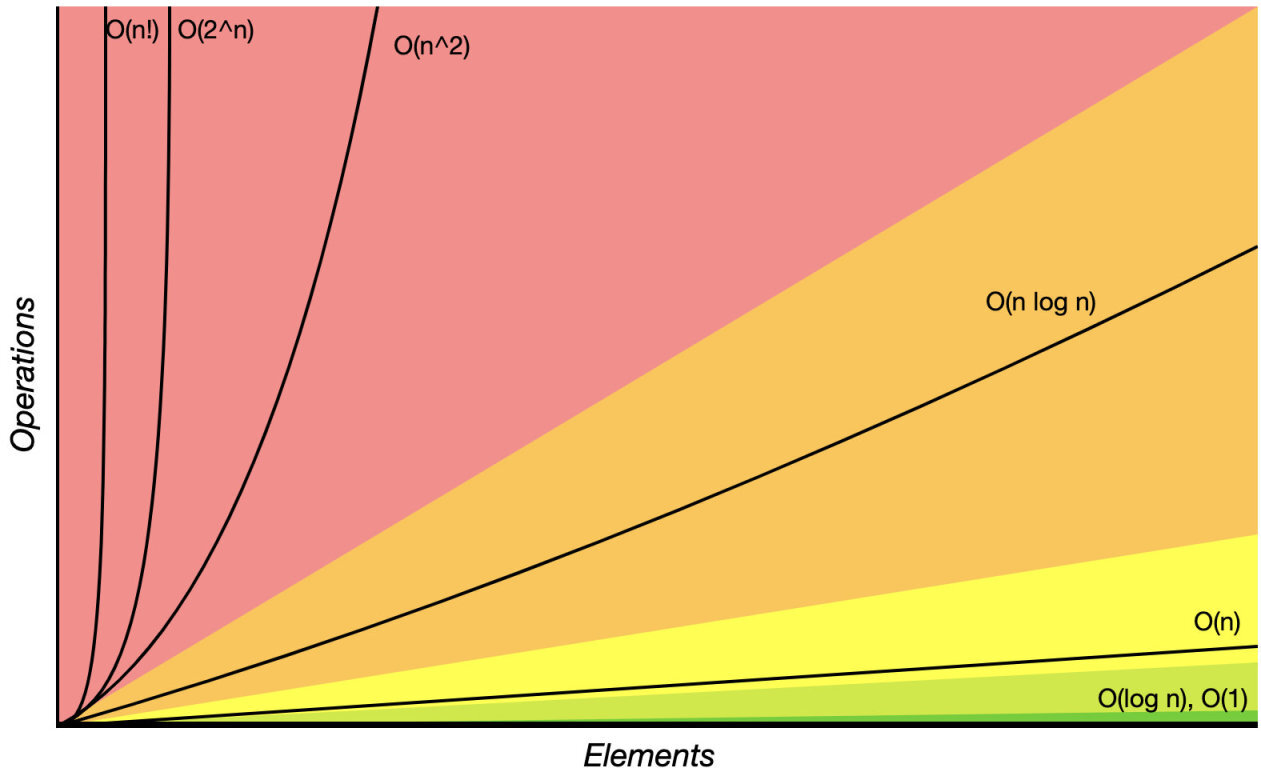
\includegraphics[width=.9\linewidth]{./pic/bigo.jpeg}

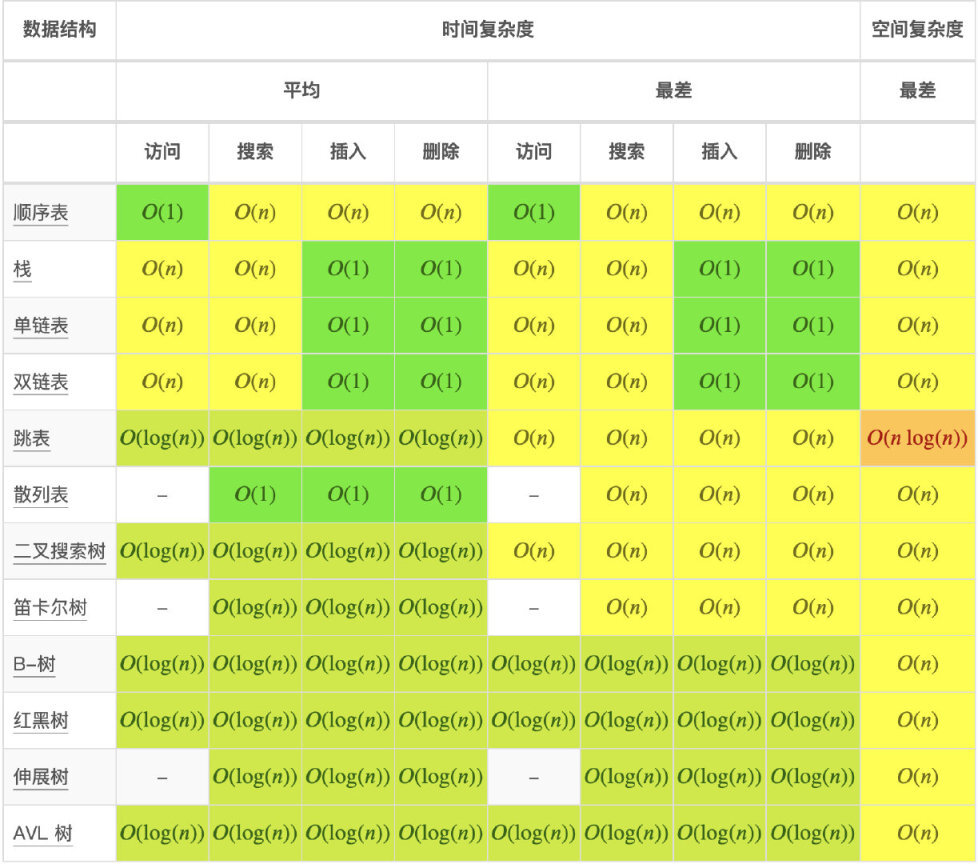
\includegraphics[width=.9\linewidth]{./pic/bigo2.jpeg}

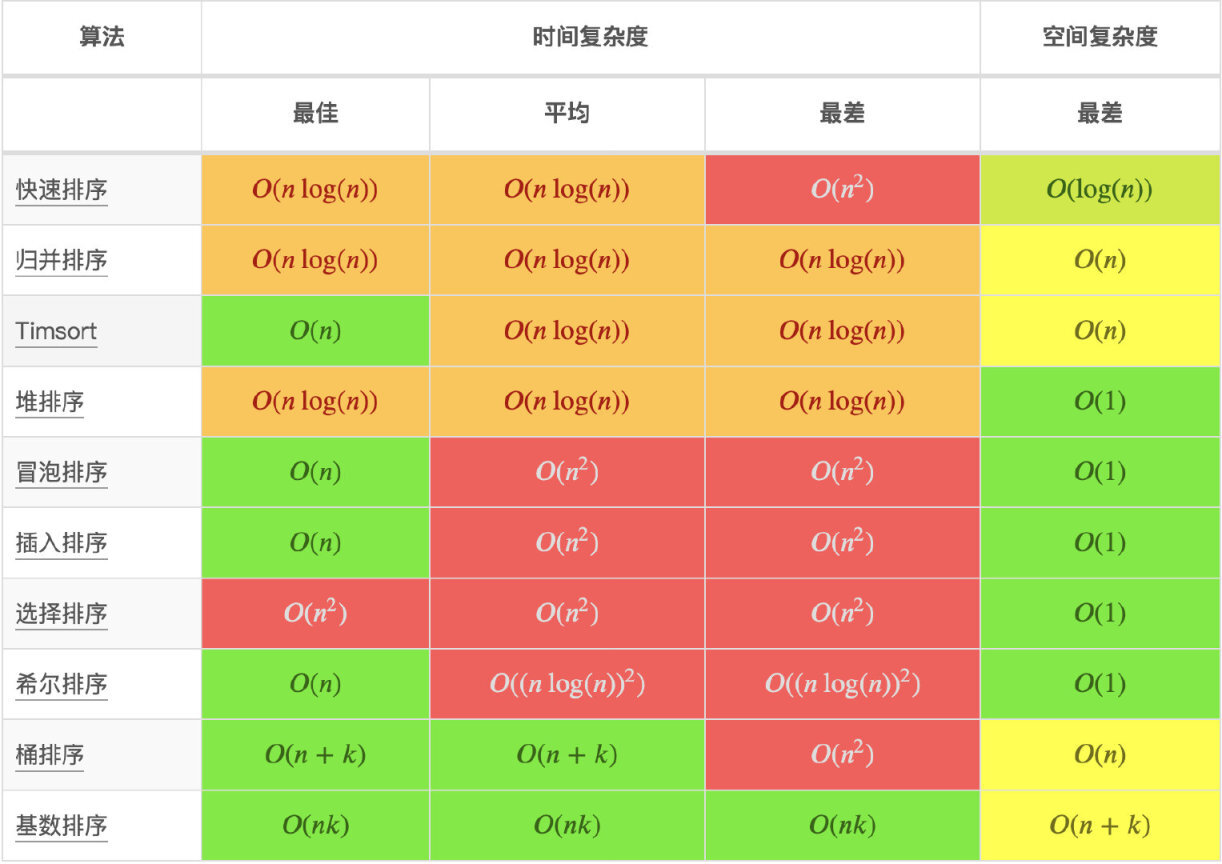
\includegraphics[width=.9\linewidth]{./pic/bigo3.jpeg}

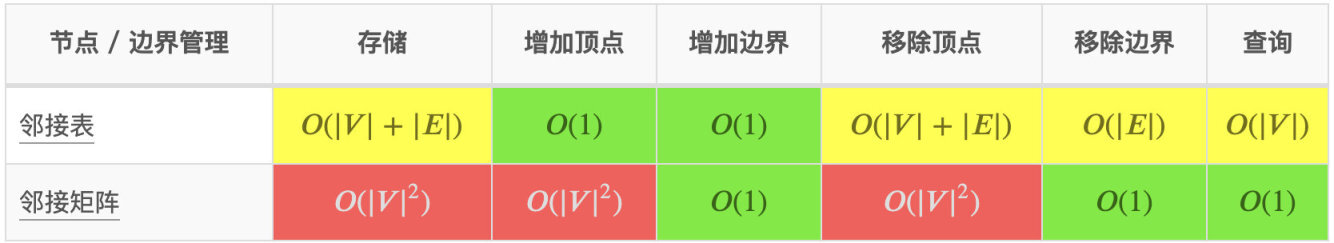
\includegraphics[width=.9\linewidth]{./pic/bigo4.jpeg}

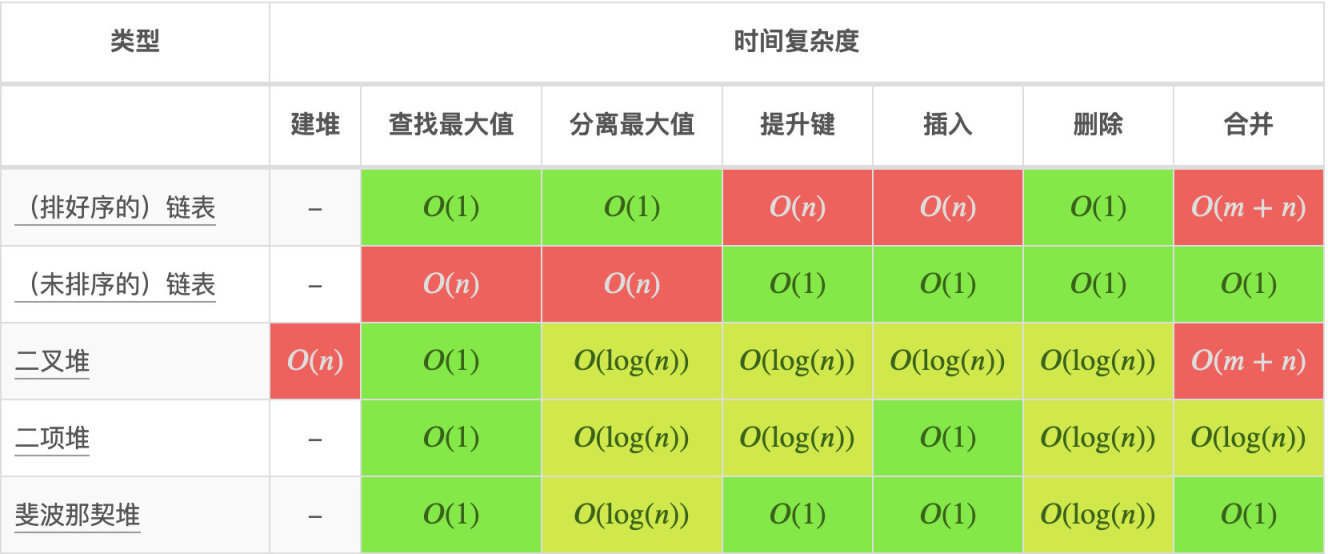
\includegraphics[width=.9\linewidth]{./pic/bigo5.jpeg}

\chapter{Dynamic Programming, 动态规划}
\label{sec-2}
\section{总结}
\label{sec-2-1}
\begin{itemize}
\item 根据CLRS,动态规划分为两种:
\item top-down with memoization (递归记忆化搜索)
\end{itemize}
等价于带缓存的,搜索树上的 DFS
比较贴近于新问题正常的思考习惯
\begin{itemize}
\item bottom-up (自底向上循环迭代)
\end{itemize}
以 "reverse topological order" 处理
每个子问题下面依赖的所有子问题都算完了才开始计算当前
一般依赖于子问题之间天然的 "size

\section{198. House Robber - Medium}
\label{sec-2-2}
You are a professional robber planning to rob houses along a street. Each house has a certain amount of money stashed, the only constraint stopping you from robbing each of them is that adjacent houses have security systems connected and it will automatically contact the police if two adjacent houses were broken into on the same night.

Given an integer array nums representing the amount of money of each house, return the maximum amount of money you can rob tonight without alerting the police.
\subsection{解题思路与分析}
\label{sec-2-2-1}
\begin{itemize}
\item 对于每一个住户来说,只有两种选择:
\begin{itemize}
\item 偷这一户人家的,下一家不要
\item 不偷这一家的,去偷下一家的
\end{itemize}
\end{itemize}
\begin{minted}[frame=lines,fontsize=\scriptsize,linenos=false]{java}
private int dfs(int [] arr, int idx) {
    if (idx >= n) return 0;
    if (dp[idx] > 0) return dp[idx];
    return dp[idx] = Math.max(dfs(arr, idx+2) + arr[idx], dfs(arr, idx+1)); // 不要忘记记忆——记住答案!!!
}
int [] dp;
int n;
public int rob(int[] a) {
    if (Arrays.stream(a).sum() == 0) return 0;
     n = a.length;
     dp = new int [n];
     return dfs(a, 0);
}
\end{minted}
\section{213. House Robber II}
\label{sec-2-3}
You are a professional robber planning to rob houses along a street. Each house has a certain amount of money stashed. All houses at this place are arranged in a circle. That means the first house is the neighbor of the last one. Meanwhile, adjacent houses have a security system connected, and it will automatically contact the police if two adjacent houses were broken into on the same night.
Given an integer array nums representing the amount of money of each house, return the maximum amount of money you can rob tonight without alerting the police.
\subsection{解题思路与分析}
\label{sec-2-3-1}
\begin{itemize}
\item 与上一题不同的是:因为是环形数组,数组首尾相连,相邻的两户人家只能偷一家
\item 问题就转化成了:我要么去偷[0, n-2]这些人家的,要么去偷[1, n-1]这些人家的,包括首尾
\item 这成了上一题的稍微变形与套娃
\end{itemize}
\begin{minted}[frame=lines,fontsize=\scriptsize,linenos=false]{java}
private int dfs(int [] arr, int i, int j, int idx) {
    if (idx > j) return 0;
    if (dp[idx] != -1) return dp[idx];
    return dp[idx] = Math.max(dfs(arr, i, j, idx+2) + arr[idx], dfs(arr, i, j, idx+1));
}
int [] dp;
int n;
public int rob(int[] arr) {
     n = arr.length;
     if (n == 1) return arr[0];
     dp = new int [n];
     Arrays.fill(dp, -1);
     int max = dfs(arr, 1, n-1, 1);
     Arrays.fill(dp, -1); // 不要忘了dp数组的重置与重新计算
     // return Math.max(dfs(arr, 1, n-1, 1), dfs(arr, 0, n-2, 0)); // BUG: 因为dp数组不重置,会发生数据混淆,得到错误答案
     return Math.max(max, dfs(arr, 0, n-2, 0));
}
\end{minted}
\section{740. Delete and Earn: 一类题目,变形了你还认得出来吗?}
\label{sec-2-4}
You are given an integer array nums. You want to maximize the number of points you get by performing the following operation any number of times:
Pick any nums[i] and delete it to earn nums[i] points. Afterwards, you must delete every element equal to nums[i] - 1 and every element equal to nums[i] + 1.
Return the maximum number of points you can earn by applying the above operation some number of times.
\subsection{解题思路与分析}
\label{sec-2-4-1}
\begin{itemize}
\item 关键题意理解:对于nums = [2, 2, 3, 3, 3, 4],如果我们选了数字3,则要删除每一个(所有)2和4,之后数组变为[3, 3],此时如果再选3,并不会删除其他元素,剩余数组变为\footnote{DEFINITION NOT FOUND.},再选3,数组变为空,返回结果是3+3+3=9。
\item 将上面的例子转化为House Robber的形式,nums' = [0, 0, 22, 33, 4],nums'[i]代表值为i的数字的总数和(或者数字(下标)i在原数组中出现的次数),每次若选择nums'数组的一个元素,则相邻元素不能在下一次被选中(包括其所有的重复计数),相当于被全部删去。转化后,用House Robber的思路来处理nums'数组即可。
\end{itemize}
\begin{minted}[frame=lines,fontsize=\scriptsize,linenos=false]{java}
private int dfs(int [] cnt, int i) {
    if (i >= N) return 0;
    if (dp[i] > 0) return dp[i];
    return dp[i] = Math.max(dfs(cnt, i+2) + cnt[i]*i, dfs(cnt, i+1));
}
int [] dp;
int N;
public int deleteAndEarn(int[] nums) {
    int n = nums.length, max = Arrays.stream(nums).max().getAsInt();
    N = max+1;
    int [] cnt = new int [N];
    for (Integer v : nums) 
        cnt[v]++;
    dp = new int [N];
    int i = 0;
    while (i < N && cnt[i] == 0) i++;
    return dfs(cnt, i);
}
\end{minted}
\begin{itemize}
\item dp解
\end{itemize}
\begin{minted}[frame=lines,fontsize=\scriptsize,linenos=false]{java}
public int deleteAndEarn(int[] nums) {
    int n = nums.length, N = 10001;
    int [] cnt = new int [N];
    for (Integer v : nums) 
        cnt[v] += v;
    int preOne = 0, preTwo = 0, ans = 0; // 相当于是滚动数组,把一维dp压缩为两个位置
    for (Integer v : cnt) {
        ans = Math.max(preOne, v + preTwo);
        preTwo = preOne;
        preOne = ans;
    }
    return ans;
}
\end{minted}


\section{2019. The Score of Students Solving Math Expression - Hard 有人说这是区间dp,无感}
\label{sec-2-5}
You are given a string s that contains digits 0-9, addition symbols '+', and multiplication symbols '*' only, representing a valid math expression of single digit numbers (e.g., 3+5*2). This expression was given to n elementary school students. The students were instructed to get the answer of the expression by following this order of operations:

Compute multiplication, reading from left to right; Then,
Compute addition, reading from left to right.
You are given an integer array answers of length n, which are the submitted answers of the students in no particular order. You are asked to grade the answers, by following these rules:

If an answer equals the correct answer of the expression, this student will be rewarded 5 points;
Otherwise, if the answer could be interpreted as if the student applied the operators in the wrong order but had correct arithmetic, this student will be rewarded 2 points;
Otherwise, this student will be rewarded 0 points.
Return the sum of the points of the students.
\subsection{解题思路与分析}
\label{sec-2-5-1}
\begin{itemize}
\item 思路是记忆化搜索。先求一下正确答案,然后开始算所有可能得到的错误答案。枚举运算符,然后递归求解两边可能的答案,汇总成当前表达式可能得到的答案。用记忆化的方式避免重复计算。
\item 时间复杂度O(l$_{\text{s}}^{\text{3}}$+l$_{\text{A}}$)),空间O(l$_{\text{s}}^{\text{2}}$)。注意有1000这个限制,上面所说的复杂度的常数是1000$^{\text{2,是很大的}}$
\end{itemize}

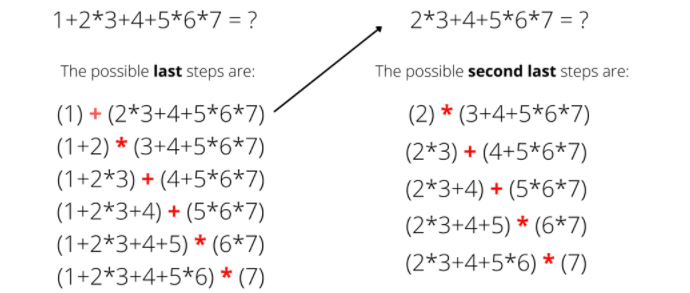
\includegraphics[width=.9\linewidth]{./pic/score.png}

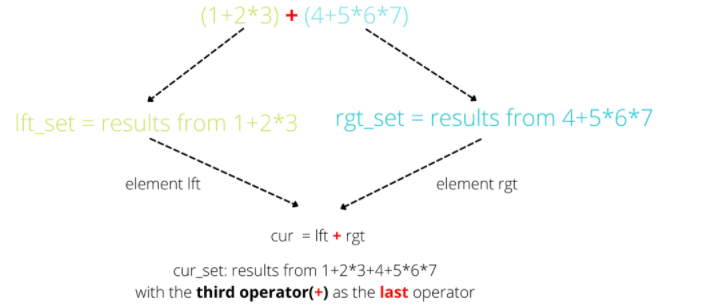
\includegraphics[width=.9\linewidth]{./pic/score2.png}

\begin{minted}[frame=lines,fontsize=\scriptsize,linenos=false]{java}
private int compute(String t) {
    ArrayDeque<Integer> st = new ArrayDeque<>();
    char [] s = t.toCharArray();
    for (int i = 0; i < s.length; i++) {
        char c = s[i];
        if (Character.isDigit(c)) 
            if (i > 0 && s[i-1] == '*') 
                st.push(st.pop() * (c-'0'));
            else st.push(c-'0');
    }
    int ans = 0;
    while (!st.isEmpty()) 
        ans += st.pop();
    return ans;
}
Set<Integer> dfs(String t, int l, int r, Set<Integer> [][] f) {
    if (f[l][r] != null) return f[l][r]; // 有记忆则调取记忆
    char [] s = t.toCharArray();
    int n = t.length(), v = 0;
    f[l][r] = new HashSet<>();
    if (l == r) {
        f[l][r].add(s[l] - '0');
        return f[l][r];
    }
    for (int i = l+1; i < r; i++) 
        if (!Character.isDigit(s[i])) { // 递归求解左右两边可能算出的答案
            Set<Integer> left = dfs(t, l, i-1, f);
            Set<Integer> right = dfs(t, i+1, r, f);
            for (Integer va : left) 
                for (Integer vb : right) {
                    if (s[i] == '*') v = va * vb;
                    else v = va + vb;
                    if (v >= 0 && v <= 1000) f[l][r].add(v);
                }
        }
    return f[l][r];
}
public int scoreOfStudents(String s, int [] num) { 
    int m = num.length, res = compute(s), n = s.length(), ans = 0;
    Set<Integer> [][] f = new HashSet[n][n]; // 第一次见,学习一下
    dfs(s, 0, n-1, f);
    Set<Integer> can = f[0][n-1];        // candidates: of wrong answers
    for (Integer v : num) 
        if (v == res) ans += 5;
        else if (can.contains(v)) ans += 2;
    return ans;
}
\end{minted}

\section{312. Burst Balloons 区间型动态规划的典型代表}
\label{sec-2-6}
You are given n balloons, indexed from 0 to n - 1. Each balloon is painted with a number on it represented by an array nums. You are asked to burst all the balloons.
If you burst the ith balloon, you will get nums[i - 1] * nums[i] * nums[i + 1] coins. If i - 1 or i + 1 goes out of bounds of the array, then treat it as if there is a balloon with a 1 painted on it.
Return the maximum coins you can collect by bursting the balloons wisely.
\begin{minted}[frame=lines,fontsize=\scriptsize,linenos=false]{java}
public int maxCoins(int[] nums) {
    int n = nums.length;
    int [][]  dp = new int [n+2][n+2];
    int [] arr = new int [n+2];
    System.arraycopy(nums, 0, arr, 1, n);
    arr[0] = arr[n+1] = 1;  // [0, n+1] ==> [1, n]
    int j = 0;
    for (int len = 1; len <= n; len++) { // [1, n]
        for (int i = 1; i+len-1 <= n; i++) { // [1, n]
            j = i + len - 1;
            for (int k = i; k <= j; k++) 
                dp[i][j] = Math.max(dp[i][j], dp[i][k-1] + dp[k+1][j] + arr[i-1]*arr[k]*arr[j+1]);
        }
    }
    return dp[1][n];
}
// 0    0    0    0    0    0
// 0    3    30   159  167  0
// 0    0    15   135  159  0
// 0    0    0    40   48   0
// 0    0    0    0    40   0
// 0    0    0    0    0    0
private int memorizedSearch(int [] arr, int x, int y) {
    if (dp[x][y] > 0) return dp[x][y];
    // if (x == y) return dp[x][y] = arr[x]; // 没有这些个边际条件
    // if (x == y-1) 
    //     return dp[x][y] = arr[x] * arr[y] + Math.max(arr[x], arr[y]);
    int max = 0;
    for (int i = x; i <= y; i++) {
        max = Math.max(max, memorizedSearch(arr, x, i-1) + memorizedSearch(arr, i+1, y) + arr[x-1]*arr[i]*arr[y+1]);
    }
    return dp[x][y] = max;
}
int [][] dp;
int n;
public int maxCoins(int[] nums) {
    int n = nums.length + 2;
    dp = new int [n][n];
    int [] arr = new int [n];
    System.arraycopy(nums, 0, arr, 1, n-2);
    arr[0] = arr[n-1] = 1;
    return memorizedSearch(arr, 1, n-2);
}
\end{minted}


\section{1866. Number of Ways to Rearrange Sticks With K Sticks Visible - Hard}
\label{sec-2-7}
There are n uniquely-sized sticks whose lengths are integers from 1 to n. You want to arrange the sticks such that exactly k sticks are visible from the left. A stick is visible from the left if there are no longer sticks to the left of it.

For example, if the sticks are arranged [1,3,2,5,4], then the sticks with lengths 1, 3, and 5 are visible from the left.
Given n and k, return the number of such arrangements. Since the answer may be large, return it modulo 109 + 7.
\begin{minted}[frame=lines,fontsize=\scriptsize,linenos=false]{java}
// dp[i][j] 表示前面i根木棍可以看到j根
// 设 dp[i][j] 表示从高度为 1, 2, ..., i 的木棍中,高度逐渐递减地插入新的木棍,从左侧看恰好看到 k 根木棍的方案数。
// 后面说看到ith根,不是指从小到大的第ith根棍子,而是指ith这个位置上的棍子
// 如果可以看到ith根的话,那么数量为dp[i-1][j-1]
// 如果看不到ith的话,那么取前面(i-1)里面任意一个出来放在ith的最后,接下来就是从前面i-1个棍子里面看到j根,所以结果是 (i-1)* dp[i-1][j]
public int rearrangeSticks(int n, int k) {
    int mod = (int)1e9 + 7;
    long [][] dp = new long [n+1][k+1];
    dp[0][0] = 1;
    for (int i = 1; i <= n; i++) 
        for (int j = 1; j <= Math.min(n, k); j++) 
            dp[i][j] = (dp[i-1][j-1] + (dp[i-1][j] * (i-1)) % mod) % mod;
    return (int)dp[n][k];
}
\end{minted}
\begin{itemize}
\item dfs + memo
\end{itemize}
\begin{minted}[frame=lines,fontsize=\scriptsize,linenos=false]{java}
long mod = 1000_000_000 + 7;
long[][] dp;
public int rearrangeSticks(int n, int k) {
    dp = new long[n + 1][k + 1];
    long ans = dfs(n, k);
    return (int) (ans % mod);
}
long dfs(int n, int k) {
    if(n < k || k == 0) return 0;
    if(n == k) return 1;
    if(dp[n][k] != 0) return dp[n][k];
    long ans = 0;
    // instead of iterating for every stick
    // we are just multiplying number of ways with (n - 1)
    ans += (((n - 1) * dfs(n - 1, k)) % mod);
    ans %= mod;
    ans += dfs(n - 1, k - 1);
    ans %= mod;
    return dp[n][k] = ans;
}
\end{minted}

\section{1916. Count Ways to Build Rooms in an Ant Colony - Hard}
\label{sec-2-8}
You are an ant tasked with adding n new rooms numbered 0 to n-1 to your colony. You are given the expansion plan as a 0-indexed integer array of length n, prevRoom, where prevRoom[i] indicates that you must build room prevRoom[i] before building room i, and these two rooms must be connected directly. Room 0 is already built, so prevRoom\footnote{DEFINITION NOT FOUND.} = -1. The expansion plan is given such that once all the rooms are built, every room will be reachable from room 0.

You can only build one room at a time, and you can travel freely between rooms you have already built only if they are connected. You can choose to build any room as long as its previous room is already built.

Return the number of different orders you can build all the rooms in. Since the answer may be large, return it modulo 109 + 7.

对每个节点,可根据所有以其子节点为根的树的节点及排列数量,计算出以当前节点为根的树的节点及排列数量。

本题求解过程涉及较多前置知识点,包括排列组合、乘法逆元、快速乘方等

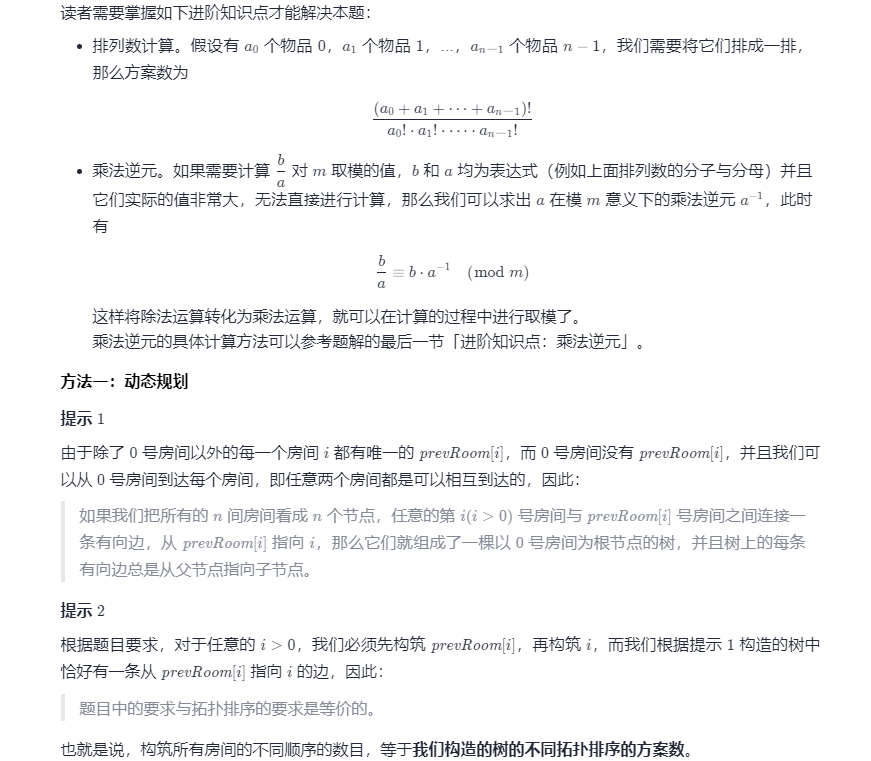
\includegraphics[width=.9\linewidth]{./pic/ant1.png}

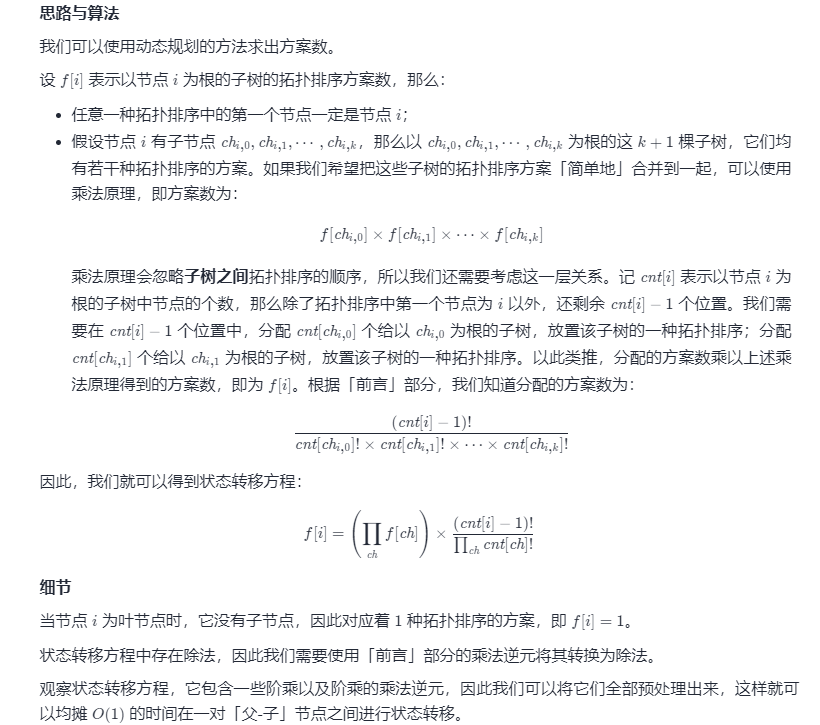
\includegraphics[width=.9\linewidth]{./pic/ant2.png}

\begin{minted}[frame=lines,fontsize=\scriptsize,linenos=false]{java}
// 快速计算x^y的乘方
public int quickMul(int x , int y) {
    long res = 1, cur = x;
    while (y > 0) {
        if ((y & 1) == 1)
            res = res * cur % mod;
        cur = cur * cur % mod;
        y >>= 1;
    }
    return (int)res;
}
// 深度优先搜索,返回以当前节点为根的子树节点个数 及 内部排列数
public int [] dfs (int idx) {
    if (!map.containsKey(idx)) return new int [] {1, 1}; // 子节点,节点个数及内部排列数均为1
    int cnt = 1, res = 1;       //  子树的节点个数、内部排列数
    for (Integer node : map.get(idx)) {
      int [] cur = dfs(node); // 递归得到子节点对应树的节点个数和排列数
        cnt += cur[0];
        res = (int)((long)res * cur[1] % mod * inv[cur[0]] % mod);
    }
    res = (int)((long)res * fac[cnt-1] % mod);
    return new int [] {cnt, res};
}
int mod = (int)1e9 + 7;
Map<Integer, List<Integer>> map = new HashMap<>();
int [] fac, inv;
public int waysToBuildRooms(int[] prevRoom) {
    int n = prevRoom.length;
    // 求阶乘数列及对应逆元
    this.fac = new int [n]; // fac[i]=i!
    this.inv = new int [n]; // inv[i]=i!^(-1)
    fac[0] = inv[0] = 1;
    for (int i = 1; i < n; i++) {
        fac[i] = (int)((long)fac[i-1] * i % mod);
        inv[i] = quickMul(fac[i], mod - 2); // 费马小定理: (fac[i]^(-1))%mod = (fac[i]^(mod-2))%mod
    }
    // 记录各个节点与子节点之间的边
    for (int i = 1; i < n; i++) 
        map.computeIfAbsent(prevRoom[i], k->new ArrayList<>()).add(i);
    // 动态规划得到总体顺序数量x
    return dfs(0)[1];      
}
\end{minted}

\section{1987. Number of Unique Good Subsequences - Hard}
\label{sec-2-9}
You are given a binary string binary. A subsequence of binary is considered good if it is not empty and has no leading zeros (with the exception of "0").

Find the number of unique good subsequences of binary.

For example, if binary = "001", then all the good subsequences are ["0", "0", "1"], so the unique good subsequences are "0" and "1". Note that subsequences "00", "01", and "001" are not good because they have leading zeros.
Return the number of unique good subsequences of binary. Since the answer may be very large, return it modulo 109 + 7.

A subsequence is a sequence that can be derived from another sequence by deleting some or no elements without changing the order of the remaining elements.
\begin{minted}[frame=lines,fontsize=\scriptsize,linenos=false]{java}
public int numberOfUniqueGoodSubsequences(String binary) {
    int mod = (int)1e9 + 7;
    int n = binary.length(), preZoo = 0, preOne = 0, m = 1;
    long [] dp = new long [n+1];
    String s = "#" + binary;
    while (m <= n && s.charAt(m) == '0') m++;
    if (m == n+1) return 1;
    dp[m] = 1;
    preOne = m;
    preZoo = m-1;
    for (int i = m+1; i <= n; i++) {
        char c = s.charAt(i);
        int j = (c == '0' ? preZoo : preOne);
        dp[i] = (2 * dp[i-1] % mod - (j >= 1 ? dp[j-1] : 0) + mod) % mod;
        if (c == '0') preZoo = i;
        else preOne = i;
    }
    return (int)dp[n] + (s.indexOf("0") != -1 ?  1 : 0);
}
\end{minted}
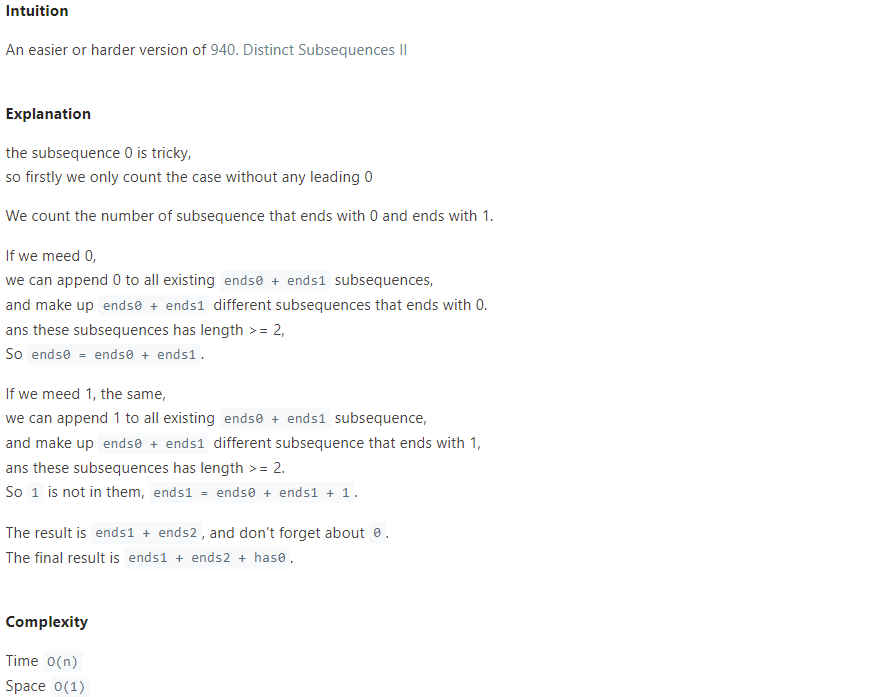
\includegraphics[width=.9\linewidth]{./pic/distinctSubsequence.png}
\begin{minted}[frame=lines,fontsize=\scriptsize,linenos=false]{java}
public int numberOfUniqueGoodSubsequences(String binary) {
    int mod = (int)1e9 + 7;
    int endZoo = 0, endOne = 0, hasZoo = 0;
    for (int i = 0; i < binary.length(); i++) 
        if (binary.charAt(i) == '1')
            endOne = (endOne + endZoo + 1) % mod;
        else {
            endZoo = (endZoo + endOne) % mod;
            hasZoo = 1;
        }
    return (endOne + endZoo + hasZoo) % mod;
}
\end{minted}
\begin{itemize}
\item 还有一个没有看懂的
\begin{itemize}
\item \url{https://leetcode-cn.com/problems/number-of-unique-good-subsequences/solution/ju-yi-fan-san-by-avenger-h-34xa/}
\item \url{https://leetcode-cn.com/problems/distinct-subsequences-ii/solution/dong-tai-gui-hua-cong-fen-xi-dao-shi-xian-by-my10y/}
\end{itemize}
\end{itemize}
\begin{minted}[frame=lines,fontsize=\scriptsize,linenos=false]{python}
def numberOfUniqueGoodSubsequences(self, binary: str) -> int:
        M = 10**9+7
        dp = [0]*10
        b = str(int(binary))
        l = len(binary) - len(b)
        if l > 0:
            dp[0] = 1
        for c in b:
            if dp[0] >= 1:
                dp[int(c)] = (sum(dp)) % M
            else:
                dp[int(c)] = ( 1+ sum(dp)) % M
        return sum(dp)%M
\end{minted}
\section{730. Count Different Palindromic Subsequences - Hard}
\label{sec-2-10}
Given a string s, return the number of different non-empty palindromic subsequences in s. Since the answer may be very large, return it modulo 109 + 7.

A subsequence of a string is obtained by deleting zero or more characters from the string.

A sequence is palindromic if it is equal to the sequence reversed.

Two sequences a1, a2, \ldots{} and b1, b2, \ldots{} are different if there is some i for which ai != bi.

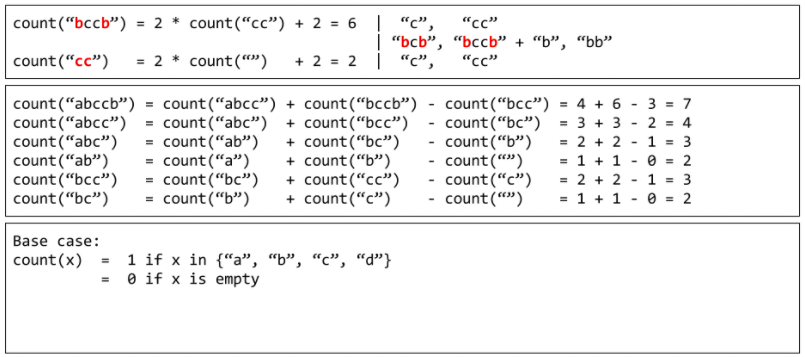
\includegraphics[width=.9\linewidth]{./pic/palindromSubSeq.png}

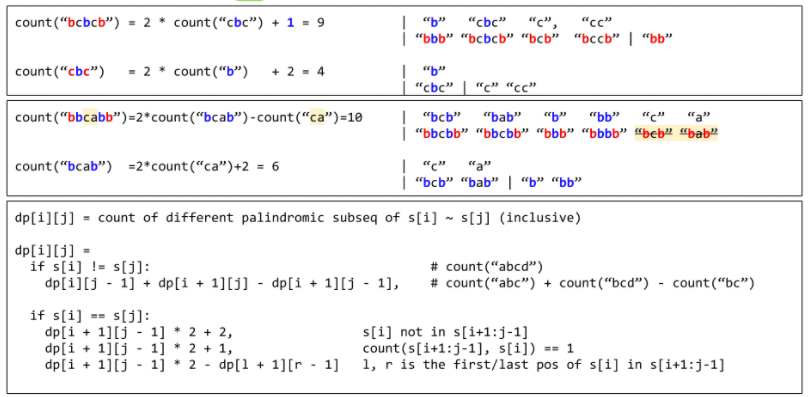
\includegraphics[width=.9\linewidth]{./pic/palindromSubSeq2.png}

\begin{minted}[frame=lines,fontsize=\scriptsize,linenos=false]{java}
private int dfs(char[] s, int i, int j) {
    if (i > j) return 0;
    if (i == j) return 1;
    if (dp[i][j] > 0) return dp[i][j];
    long ans = 0;
    if (s[i] == s[j]) {
        ans += dfs(s, i + 1, j - 1) * 2;
        int l = i + 1;
        int r = j - 1;
        while (l <= r && s[l] != s[i]) ++l;
        while (l <= r && s[r] != s[i]) --r;
        if (l > r) ans += 2;
        else if (l == r) ans += 1;
        else ans -= dfs(s, l + 1, r - 1);
    } else 
        ans = dfs(s, i, j - 1) + dfs(s, i + 1, j) - dfs(s, i + 1, j - 1);
    return dp[i][j] = (int)((ans + mod) % mod);
}
private static final int mod = (int)1e9 + 7;
private int [][] dp;
public int countPalindromicSubsequences(String S) {
    int n = S.length();
    dp = new int[n][n];
    return dfs(S.toCharArray(), 0, n - 1);
}
\end{minted}
\begin{itemize}
\item dp
\end{itemize}
\begin{minted}[frame=lines,fontsize=\scriptsize,linenos=false]{java}
public int countPalindromicSubsequences(String s) {
    int n = s.length();
    int mod = (int)1e9 + 7;
    char [] arr = s.toCharArray();
    long [][] dp = new long [n][n];
    for (int i = 0; i < n; i++) 
        dp[i][i] = 1;
    for (int len = 1; len <= n; len++) {
        for (int i = 0; i+len < n; i++) {
            int j = i + len;
            if (arr[i] == arr[j]) {
                dp[i][j] = dp[i+1][j-1] * 2;
                int l = i+1;
                int r = j-1;
                while (l <= r && arr[l] != arr[i]) ++l;
                while (l <= r && arr[r] != arr[i]) --r;
                if (l == r) dp[i][j] += 1;
                else if (l > r) dp[i][j] += 2;
                else dp[i][j] -= dp[l+1][r-1];
            } else dp[i][j] = dp[i][j-1] + dp[i+1][j] - dp[i+1][j-1];
            dp[i][j] = (dp[i][j] + mod) % mod;
        }
    }
    return (int)dp[0][n-1];
}
\end{minted}

\section{1125. Smallest Sufficient Team - Hard 这个题要多写几遍}
\label{sec-2-11}
In a project, you have a list of required skills req$_{\text{skills}}$, and a list of people. The ith person people[i] contains a list of skills that the person has.

Consider a sufficient team: a set of people such that for every required skill in req$_{\text{skills}}$, there is at least one person in the team who has that skill. We can represent these teams by the index of each person.

For example, team = [0, 1, 3] represents the people with skills people\footnotemark[2]{}, people\footnote{DEFINITION NOT FOUND.}, and people\footnotemark[1]{}.
Return any sufficient team of the smallest possible size, represented by the index of each person. You may return the answer in any order.

It is guaranteed an answer exists.
\begin{minted}[frame=lines,fontsize=\scriptsize,linenos=false]{java}
// 强行剪枝: 收集到的size >= 目前的结果,直接return;
// 这题的思路就是先把skill 和set of people建立好,
// 然后去用skill set做backtracking收集,如果temp team的size大于结果,直接return,否则update结果,
// 这里有个小tricky的地方,就是如果people是新人,加入之后dfs,backtracking的时候,要判断如果是新人,则remove,否则不remove;
private void dfs(String[] req_skills, HashSet<Integer> team, int idx) {
    if (team.size() >= minTeamSize) return; // 强行剪枝: 收集到的size >= 目前的结果,直接return;
    if (idx == req_skills.length) {
        minTeamSize = team.size();
        resTeam = new HashSet<Integer>(team);
        return;
    }
    boolean isNewPerson = false;
    for (int people : map.get(req_skills[idx])) {
        isNewPerson = team.add(people);
        dfs(req_skills, team, idx + 1);
        if (isNewPerson)
            team.remove(people);
    }
}
HashMap<String, Set<Integer>> map;
Set<Integer> resTeam; 
int minTeamSize;
public int[] smallestSufficientTeam(String[] req_skills, List<List<String>> people) {
    minTeamSize = people.size();
    this.map = new HashMap<>(); 
    for (int i = 0; i < minTeamSize; i++) 
        for (String skill: people.get(i)) 
            map.computeIfAbsent(skill, k -> new HashSet<Integer>()).add(i);
    this.resTeam = new HashSet<Integer>();
    dfs(req_skills, new HashSet<Integer>(), 0);
    int [] res = new int[resTeam.size()];     
    int idx = 0;
    for (int person : resTeam) 
        res[idx++] = person;
    return res;
}
\end{minted}
\begin{itemize}
\item Java soution using Bit DP 10ms
\end{itemize}
\begin{minted}[frame=lines,fontsize=\scriptsize,linenos=false]{java}
public int[] smallestSufficientTeam(String[] req_skills, List<List<String>> people) {
    int n = req_skills.length, range = 1 << n, cur, idx;
    Map<String, Integer> idxMap = new HashMap<>();
    for (int i = 0; i < n; i++) 
        idxMap.put(req_skills[i], i);
    long [] dp = new long [range]; // 每个bit位实际存了构成答案最小组的各成员的下标, 60个人, long
    int [] cnt = new int [range];
    Arrays.fill(cnt, Integer.MAX_VALUE);
    cnt[0] = 0;
    for (int i = 0; i < people.size(); i++) {
        List<String> l = people.get(i);
        cur = 0;
        for (String skill : l) 
            if (idxMap.containsKey(skill))
                cur |= 1 << idxMap.get(skill);
        for (int j = range-1; j > 0; j--) {
            idx = (j & cur) ^ j; // 由其它人所构成的拥有j的这些种技能的子集/ j的这些种技能可以由j一个人来替换(其它可能需要很多人才能最终拥有这些技能)
            if (cnt[idx] != Integer.MAX_VALUE && cnt[j] > cnt[idx] + 1) {
                cnt[j] = cnt[idx] + 1;
                dp[j] = dp[idx] | (1L << i); // at most 60 people
            }
        }
    }
    int [] res = new int[cnt[range-1]];
    long preRes = dp[range-1]; // 5 people: 11111, 1111, 111, 11, 1
    int valIdx = 0;
    long val = 0;
    idx = 0;
    while (preRes != 0) {
        val = preRes & 1;
        if (val == 1) res[idx++] = valIdx;
        preRes >>= 1;
        valIdx++;
    }
    return res;
}
\end{minted}
\begin{itemize}
\item DFS + Memorizaion (A real O(2$^{\text{skill}}$ * people) Solution) Java 8ms
\begin{itemize}
\item \url{https://leetcode.com/problems/smallest-sufficient-team/discuss/1011135/DFS-\%2B-Memorizaion}-(A-real-O(2skill-*-people)-Solution)-Java-8ms
\end{itemize}
\end{itemize}
\begin{minted}[frame=lines,fontsize=\scriptsize,linenos=false]{java}
List<Integer> minComb;
int[] peopleSkillMasks;
Integer[] memo;  // 这个方法确实快一点儿
int[] nextPerson;
int n;
public int[] smallestSufficientTeam(String[] req_skills, List<List<String>> people) {
    // 1. some preprocess to get bitmask for people skills
    this.n = req_skills.length;
    Map<String, Integer> skillToIdx = new HashMap<>();
    for (int i = 0; i < n; i++) 
        skillToIdx.put(req_skills[i], i);
    this.peopleSkillMasks = new int[people.size()];
    for (int i = 0; i < peopleSkillMasks.length; i++) {
        int skillMask = 0;
        for (String skill : people.get(i)) 
            skillMask |= (1 << skillToIdx.get(skill));
        peopleSkillMasks[i] = skillMask;
    }
    // 2. dfs
    memo = new Integer[1 << n];
    nextPerson = new int[1 << n];
    dfs(0, 0);
    // 3. reconstruct the path
    int curSkillSet = 0;
    List<Integer> res = new ArrayList<>();
    while(curSkillSet != (1 << n) - 1) {
        res.add(nextPerson[curSkillSet]);
        curSkillSet |= peopleSkillMasks[nextPerson[curSkillSet]];
    }
    return res.stream().mapToInt(i->i).toArray();
}
// a very simple dfs with memo to compute all combinations of people. 
// Use memorization to optimize the time complexity to O(2^skill * people) 2^skill for 2^skill node in the tree, people because each node has people computation
private int dfs(int curSkillSet, int startIdx) {
    if (curSkillSet == (1 << n) - 1) return 0;
    if (memo[curSkillSet] == null) {
        int res = Integer.MAX_VALUE / 2;
        int nextPersonIdx = -1;
        for (int i = startIdx; i < peopleSkillMasks.length; i++) {
            int withNewSkill = peopleSkillMasks[i] | curSkillSet; 
            if (withNewSkill != curSkillSet) {
                int numPeople = dfs(withNewSkill, i+1) + 1;
                if (res > numPeople) {
                    res = numPeople;
                    nextPersonIdx = i;
                }
            }
        }
        memo[curSkillSet] = res;
        nextPerson[curSkillSet] = nextPersonIdx; 
    }
    return memo[curSkillSet];
}
\end{minted}
\begin{itemize}
\item Recursion + Memoization + bit mask , with Simple JAVA solution
\begin{itemize}
\item \url{https://leetcode.com/problems/smallest-sufficient-team/discuss/1487180/Recursion-\%2B-Memoization-\%2B-bit-mask-with-Simple-JAVA-solution}
\end{itemize}
\end{itemize}
上面的这些方法相对较偏,就暂时顾不上了

\section{1575. Count All Possible Routes - Hard}
\label{sec-2-12}
You are given an array of distinct positive integers locations where locations[i] represents the position of city i. You are also given integers start, finish and fuel representing the starting city, ending city, and the initial amount of fuel you have, respectively.

At each step, if you are at city i, you can pick any city j such that j != i and 0 <= j < locations.length and move to city j. Moving from city i to city j reduces the amount of fuel you have by |locations[i] - locations[j]|. Please notice that |x| denotes the absolute value of x.

Notice that fuel cannot become negative at any point in time, and that you are allowed to visit any city more than once (including start and finish).

Return the count of all possible routes from start to finish.

Since the answer may be too large, return it modulo 10$^{\text{9}}$ + 7.
\begin{minted}[frame=lines,fontsize=\scriptsize,linenos=false]{java}
// 自顶向下 (记忆化搜索)
// 每个dfs搜索当前状态为城市i,油量f到达终点的方案数。这样决策的时候就很直观:当前这个状态的方案数,由可去的城市的,且油量为剩余油量的到达终点方案数加起来。
// 初始化:每个状态都初始化为-1。
// 当走到终点时,这个状态的可走到终点的方案数+1。
private int dfs(int [] arr, int end, int idx, int fu) {
    if (dp[idx][fu] != -1) return dp[idx][fu];
    dp[idx][fu] = 0;
    if (idx == end) {
        dp[idx][fu] += 1;
        dp[idx][fu] %= mod;
    }
    for (int i = 0; i < n; i++) {
        if (i == idx || Math.abs(arr[i] - arr[idx]) > fu) continue;
        dp[idx][fu] = (dp[idx][fu] + dfs(arr, end, i, fu-Math.abs(arr[i]-arr[idx]))) % mod;
    }
    return dp[idx][fu];
}
int mod = (int)1e9 + 7;
int [][] dp;
int n;
public int countRoutes(int[] locations, int start, int finish, int fuel) {
    n = locations.length;
    if (fuel < Math.abs(locations[start] - locations[finish])) return 0;
    dp = new int[n][fuel+1];
    for (int i = 0; i < n; i++) 
        Arrays.fill(dp[i], -1);
    dfs(locations, finish, start, fuel);
    return dp[start][fuel];
}
// 自底向上
// 为什么想到动态规划:最优子结构:到达终点的方案数肯定由到达其他点的,不同油量的方案数求和。
//     如何定义状态:城市肯定在状态里,因为其他城市有不同的剩余油量的状态,且油量为0无法到达,也成为限制之一。所以油量也必须在状态里:
//     d p ( i , f ) dp(i, f)dp(i,f)表示到达第 i ii个城市,剩余油量为f ff 的方案数。
//     状态转移:第i ii个城市,可以由除本身外的城市转移过来,只要剩余的油量不小于所用的油量就够了,最后答案是求总共的个数,所以只要方案数相加就行:
//     dp(i,f−dist)=dp(i,f−dist)+dp(k,f)(f−dist>=0)
//     枚举顺序:每个城市肯定都要枚举一遍,因为还需要从另一个城市转移过来,所以除本身外的城市肯定还要再枚举一遍。
//     关键是油量的枚举,因为油量肯定是慢慢减少的,可以想到是逆序枚举,而且油量要放在最外层枚举。因为如果先枚举城市i ii,再枚举城市j jj,再枚举油量的话,只是不断更新了i ii城市方案数,而j jj城市不同油量的方案数根本没变化。
// dp:最优子结构 到达终点的方案数肯定由到达其他点的,不同油量的方案数求和
// 搜索:反过来 在第 i 个城市到达 fin 的方案数,也可以由其他的点到达 fin 的方案数转移过来, 但是油量有限制,所以油量肯定在状态里
// 所以城市 和 剩余油量肯定在状态里
// dp(i, j) 表示到达第 i 个城市,剩余油量为 j 的方案数
// dp(i, j) = dp(i, j) + dp(k, j - dist)
public int countRoutes(int[] locations, int start, int finish, int fuel) {
    int n = locations.length;
    if (fuel < Math.abs(locations[start] - locations[finish])) return 0;
    int [][] dp = new int[n][fuel+1];
    dp[start][fuel] = 1; // 初始点且燃料满的点方案数为1
    int leftFu = 0, mod = (int)1e9 + 7;
    for (int j = fuel; j >= 0; j--) { // fuel leftover
        for (int i = 0; i < n; i++) { // cur city
            for (int k = 0; k < n; k++) { // next city
                if (i == k) continue;
                leftFu = j - Math.abs(locations[i] - locations[k]);
                if (leftFu < 0) continue;
                dp[i][leftFu] = (dp[i][leftFu] + dp[k][j]) % mod; // 这里好别扭呀: 想呀想呀 
            }
        }
    }
    int ans = 0;
    for (int i = 0; i <= fuel; i++) 
        ans = (ans + dp[finish][i]) % mod;
    return ans;
}
\end{minted}

\section{1012. Numbers With Repeated Digits - Hard}
\label{sec-2-13}
Given an integer n, return the number of positive integers in the range [1, n] that have at least one repeated digit.

题意:统计1-N中,满足每个位置都不同的数有几个。

思路:数位DP。通过一个1<<10的mask表示当前这个数,1-9哪些数被用了。

比赛的时候,一直想通过一个dfs直接找到不重复的数,一直不对。

赛后发现,别人都是通过一个dfs找重复的数,然后总个数减去。

\begin{minted}[frame=lines,fontsize=\scriptsize,linenos=false]{java}
private int dfs(int len, int limit, int mask) { // 不重复数的个数
    if (len == 0) return 1;
    if (limit == 0 && dp[len][mask][limit] > 0) return dp[len][mask][limit]; // 记忆化部分
    int maxn = limit > 0 ? bit[len] : 9; // 求出最高可以枚举到哪个数字
    int ans = 0;
    for (int i = 0; i <= maxn; i++)  // 当前位
        if ((mask&(1 << i)) == 0)
            if (mask == 0 && i == 0)
                ans += dfs(len - 1, (limit > 0 && i == maxn ? 1 : 0), mask); // 有前导0,所以0不能统计,不更新mask
            else ans += dfs(len - 1, (limit > 0 && i == maxn ? 1 : 0), mask | (1 << i)); // 更新mask
    if (limit == 0) dp[len][mask][limit] = ans; // 如果没有限制,代表搜满了,可以记忆化,否则就不能
    return ans;
}
int [][][] dp;
int [] bit;
public int numDupDigitsAtMostN(int N) {
    int sum = N + 1;
    bit = new int [19];
    dp = new int [19][1 << 10][2];
    int idx = 0;
    while (N > 0) {
        bit[++idx] = N % 10;
        N /= 10;
    }
    return sum - dfs(idx, 1, 0);
}
\end{minted}
\begin{itemize}
\item 这道题给了一个正整数N,让返回所有不大于N且至少有一个重复数字的正整数的个数,题目中给的例子也可以很好的帮助我们理解。要求的是正整数的位数上至少要有一个重复数字,当然最简单暴力的方法就是从1遍历到N,然后对于每个数字判断是否有重复数字,看了一眼题目难度 Hard,想都不用想,肯定是超时的。这道题需要更高效的解法,首先来想,若是直接求至少有一个重复数字的正整数,由于并不知道有多少个重复数字,可能1个,2个,甚至全是重复数字,这样很难找到规律。有时候直接求一个问题不好求,可以考虑求其相反的情况,至少有一个重复数字反过来就是一个重复数字都没有,所以这里可以求不大于N且一个重复数字都没有的正整数的个数,然后用N减去这个数字即为所求。好,接下来看怎么求,对于任意一个N,比如 7918,是个四位数,而所有的三位数,两位数,一位数,都一定比其小,所以可以直接求出没有重复数字的三位数,两位数,和一位数。比如三位数,由于百位上不能有0,则只有9种情况,十位上可以有0,则有9种情况,个位上则有8种情况,所以就是 9*9*8。可以归纳出没有重复数字的n位数的个数,最高位去除0还有9种,剩余的 n-1 位则依次是 9,8,7\ldots{} 则后面的 n-1 位其实是个全排列,从9个数中取出 n-1 个数字的全排列,初中就学过的。这里写一个全排列的子函数,求从m个数字中取n个数字的全排列,方便后面计算。算完这些后,还要来算符合题意的四位数,由于第一位是7,若千位上是小于7的数字(共有6种,千位上不能是0),则后面的百位,十位,个位又都可以全排列了,从9个数字中取3个数字的全排列,再乘以千位上小于7的6种情况。若当千位固定为7,则百位上可以放小于9的数字(共有8种,百位不能放7,但可以放0),则后面的十位和个位都可以全排列了,从8个数字种取出2个数字的全排列,再乘以百位上小于9的8种情况。需要注意的是,遍历给定数字的各个位时,有可能出现重复数字,一旦出现了之后,则该 prefix 就不能再用了,因为已经不合题意了。所以要用一个 HashSet 来记录访问过的数字,一旦遇到重复数字后就直接 break 掉。最后还有一个小 trick 需要注意,由于N本身也需要计算进去,所以再计算的时候,使用 N+1 进行计算的话,就可以把N这种情况算进去了
\end{itemize}
\begin{minted}[frame=lines,fontsize=\scriptsize,linenos=false]{java}
private int A(int m, int n) {
    return n == 0 ? 1 : A(m, n-1) * (m-n+1);
}
public int numDupDigitsAtMostN(int n) {
    List<Integer> digits = new ArrayList<>();
    Set<Integer> vis = new HashSet<>();
    for (int i = n+1; i > 0; i /= 10) 
        digits.add(0, i % 10);
    int res = 0, m = digits.size();
    for (int i = 1; i < m; i++) res += 9 * A(9,  i-1);
    for (int i = 0; i < m; i++) {
        for (int j = i > 0 ? 0 : 1; j < digits.get(i); ++j) {
            if (vis.contains(j)) continue;
            res += A(9-i, m-i-1);
        }
        if (vis.contains(digits.get(i))) break;
        vis.add(digits.get(i));
    }
    return n - res;
}
\end{minted}

\section{514. Freedom Trail - Hard}
\label{sec-2-14}
In the video game Fallout 4, the quest "Road to Freedom" requires players to reach a metal dial called the "Freedom Trail Ring" and use the dial to spell a specific keyword to open the door.

Given a string ring that represents the code engraved on the outer ring and another string key that represents the keyword that needs to be spelled, return the minimum number of steps to spell all the characters in the keyword.

Initially, the first character of the ring is aligned at the "12:00" direction. You should spell all the characters in key one by one by rotating ring clockwise or anticlockwise to make each character of the string key aligned at the "12:00" direction and then by pressing the center button.

At the stage of rotating the ring to spell the key character key[i]:

You can rotate the ring clockwise or anticlockwise by one place, which counts as one step. The final purpose of the rotation is to align one of ring's characters at the "12:00" direction, where this character must equal key[i].
If the character key[i] has been aligned at the "12:00" direction, press the center button to spell, which also counts as one step. After the pressing, you could begin to spell the next character in the key (next stage). Otherwise, you have finished all the spelling.
\subsection{解题思路分析: 这个图把钥匙中每个字母的出现位置记住了,以后拿去用不搜 dfs + 记忆数组}
\label{sec-2-14-1}
\begin{itemize}
\item 记录下所有字母对应的位置,这样在找字母相对位置的时候就不需要循环搜索了
\item 采用递归的方法,找出当前字母对应的位置最小的步数:只需要把当前字母对应的所有位置找出来,然后计算最小值即可
\item 下一个位置再次迭代计算即可
\end{itemize}
\begin{minted}[frame=lines,fontsize=\scriptsize,linenos=false]{java}
public int minLen(int len, int i, int j) {
    int min = Math.min(i, j);
    int max = Math.max(i, j);
    return Math.min(Math.abs(i - j), Math.abs(len + min - max));
}
public int helper(String ring, int i, String key, int j) {
    if (j >= n) return 0;
    if (dp[i][j] > 0) return dp[i][j];
    List<Integer> nextPos = map.get(key.charAt(j));
    int min = Integer.MAX_VALUE;
    for (int k = 0; k < nextPos.size(); k++) 
        min = Math.min(min, helper(ring, nextPos.get(k), key, j+1) + minLen(m, nextPos.get(k), i) + 1);
    dp[i][j] = min;
    return dp[i][j];
}
Map<Character, List<Integer>> map = new HashMap<>(); // 这个图把钥匙中每个字母的出现位置记住了,以后拿去用不搜
int[][] dp;
int m, n;
public int findRotateSteps(String ring, String key) {
    m = ring.length();
    n = key.length();
    dp = new int[m][n];
    for (int i = 0; i < m; i++) {
        if (key.indexOf(ring.charAt(i)) == -1) continue;
        char c = ring.charAt(i);
        List<Integer> li = map.get(c);
        if (li == null) {
            li = new ArrayList<>();
            map.put(c, li);
        }
        li.add(i);
    }
    return helper(ring, 0, key, 0);
}
\end{minted}
\subsection{解题思路分析 动态规划}
\label{sec-2-14-2}
\begin{itemize}
\item 博主最先尝试的用贪婪算法来做,就是每一步都选最短的转法,但是OJ中总有些test case会引诱贪婪算法得出错误的结果,因为全局最优解不一定都是局部最优解,而贪婪算法一直都是在累加局部最优解,这也是为啥DP解法这么叼的原因。贪婪算法好想好实现,但是不一定能得到正确的结果。DP解法难想不好写,但往往才是正确的解法,这也算一个trade off吧。
\item 此题需要使用一个二维数组dp,其中dp[i][j]表示转动从i位置开始的key串所需要的最少步数(这里不包括spell的步数,因为spell可以在最后统一加上),此时表盘的12点位置是ring中的第j个字符。不得不佩服这样的设计的确很巧妙,我们可以从key的末尾往前推,这样dp\footnotemark[2]{}\textsuperscript{,}\,\footnotemark[2]{}就是我们所需要的结果,因为此时是从key的开头开始转动,而且表盘此时的12点位置也是ring的第一个字符。现在我们来看如何找出递推公式,对于dp[i][j],我们知道此时要将key[i]转动到12点的位置,而此时表盘的12点位置是ring[j],我们有两种旋转的方式,顺时针和逆时针,我们的目标肯定是要求最小的转动步数,而顺时针和逆时针的转动次数之和刚好为ring的长度n,这样我们求出来一个方向的次数,就可以迅速得到反方向的转动次数。为了将此时表盘上12点位置上的ring[j]转动到key[i],我们要将表盘转动一整圈,当转到key[i]的位置时,我们计算出转动步数diff,然后计算出反向转动步数,并取二者较小值为整个转动步数step,此时我们更新dp[i][j],更新对比值为step + dp[i+1][k],这个也不难理解,因为key的前一个字符key[i+1]的转动情况suppose已经计算好了,那么dp[i+1][k]就是当时表盘12点位置上ring[k]的情况的最短步数,step就是从ring[k]转到ring[j]的步数,也就是key[i]转到ring[j]的步数,用语言来描述就是,从key的i位置开始转动并且此时表盘12点位置为ring[j]的最小步数(dp[i][j])就等价于将ring[k]转动到12点位置的步数(step)加上从key的i+1位置开始转动并且ring[k]已经在表盘12点位置上的最小步数(dp[i+1][k])之和。
\item 突然发现这不就是之前那道Reverse Pairs中解法一中归纳的顺序重现关系的思路吗,都做了总结,可换个马甲就又不认识了,泪目中。。。
\end{itemize}
\begin{minted}[frame=lines,fontsize=\scriptsize,linenos=false]{java}
public int findRotateSteps(String ring, String key) {
    int m = key.length(); 
    int n = ring.length();
    int [][] dp = new int[m+1][n];
    int diff = 0, step = 0;
    for (int i = m-1; i >= 0; i--) {
        for (int j = 0; j < n; j++) {
            dp[i][j] = Integer.MAX_VALUE;
            for (int k = 0; k < n; k++) {
                if (ring.charAt(k) == key.charAt(i)) {
                    diff = Math.abs(j - k);
                    step = Math.min(diff, n-diff);
                    dp[i][j] = Math.min(dp[i][j], step + dp[i+1][k]);
                }
            }
        }
    }
    return dp[0][0] + m;
}
\end{minted}

\subsection{解题思路分析: dfs + 记忆数组}
\label{sec-2-14-3}
\begin{itemize}
\item 过程就是需要一步一步求key里面的每个字符。 如果当前位置已经是对应到这个字符,那么直接按按钮就可以
\item 如果当前位置不是,那么有两种旋转方式,顺时针或者逆时针, 然后找到第一个字符就是在同一个方向上的最短距离,
\item 因为在同一个方向上,即使后面有重复的字符,无论后面的字符在那里,遇到第一个符合条件的字符就按按钮一定是最优解。
\item 但是在不同方向上就不一定了,有可能一个方向上当前字符距离更短,但是有可能后面的字符距离会更远,
\begin{itemize}
\item 比如ring=ABCDEFGBF , key=BG, 如果看第一个字符, 那应该是顺时针,只需要转一格就到,逆时针需要转两格,
\item 但是顺时针第一步快了以后, 后面到G会需要更长的步骤。 而逆时针会比较快。
\end{itemize}
\item 所以,基本的逻辑是每一步不能决定当前哪个方向是否是最优解, 只有不断递归,把每步的两个方向全部尝试完到key结束才可以
\item 当然, 如果不做任何处理,这样做是要超时的(我开始就写了这样一个版本), 一个直观的做法,就是在递归的基础上
\begin{itemize}
\item 加一个记忆表, 针对ring的位置index和key的kindex做记录, 如果已经存在一个解了就可以直接返回结果
\end{itemize}
\item 这个递归+memorization的解法,那一定存在一个bottom up的动态规划解法, 这个后面再学习
\end{itemize}
\begin{minted}[frame=lines,fontsize=\scriptsize,linenos=false]{java}
private int helper(String s, String t, int i, int j) { // s: ring, t: key, i: idxRing, j: idxKey
    Map<Integer, Integer> locMap = mem.get(i);
    if (locMap != null) 
        if (locMap.get(j) != null) return locMap.get(j);
    if (j == n) return 0;
    int step = 0, k = i;
    boolean foundK = false;
    for (; step <= m/2; ++step) {
        k = (i + step + m) % m;
        if (s.charAt(k) == t.charAt(j)) {
            foundK = true;
            break;
        }
    }
    int rstep = 0, x = i;
    boolean foundX = false;
    while (rstep <= m/2) {
        x = (i - rstep + m) % m;
        if (s.charAt(x) == t.charAt(j)) {
            foundX = true;
            break;
        }
        rstep++;
    }
    int min = Integer.MAX_VALUE;
    if (foundK) min = helper(s, t, k, j+1) + step + 1;
    if (foundX) min = Math.min(min, helper(s, t, x, j+1) + rstep + 1);
    if (locMap == null) {
        locMap = new HashMap<>();
        mem.put(i, locMap);
    }
    locMap.put(j, min);
    return min;
}
Map<Integer, Map<Integer, Integer>> mem = new HashMap<>();
int m, n;
public int findRotateSteps(String ring, String key) {
    m = ring.length();
    n = key.length();
    return helper(ring, key, 0, 0);
}
\end{minted}

\section{847. Shortest Path Visiting All Nodes}
\label{sec-2-15}
You have an undirected, connected graph of n nodes labeled from 0 to n - 1. You are given an array graph where graph[i] is a list of all the nodes connected with node i by an edge.
Return the length of the shortest path that visits every node. You may start and stop at any node, you may revisit nodes multiple times, and you may reuse edges.
\begin{minted}[frame=lines,fontsize=\scriptsize,linenos=false]{java}
public int shortestPathLength(int[][] graph) {
    int n = graph.length;
    int tar = 0, res = 0;
    HashSet<String> s = new HashSet<>();
    Queue<Pair<Integer, Integer>> q = new LinkedList<>();
    for (int i = 0; i < n; i++) {
        int mask = (1 << i);
        tar |= mask;
        s.add(Integer.toString(mask) + "-" + Integer.toString(i));
        q.add(new Pair<>(mask, i));
    }
    while (!q.isEmpty()) {
        for (int i = q.size(); i > 0; i--) {
            Pair cur = q.remove();
            if ((int)cur.getKey() == tar) return res;
            for (int next : graph[(int)cur.getValue()]) {
                int path = (int)cur.getKey() | (1 << next);
                String str = Integer.toString(path) + "-" + Integer.toString(next);
                if (s.contains(str)) continue;
                s.add(str);
                q.add(new Pair<>(path, next));
            }
        }
        ++res;
    }
    return -1;
}
\end{minted}

\section{1931. Painting a Grid With Three Different Colors}
\label{sec-2-16}
You are given two integers m and n. Consider an m x n grid where each cell is initially white. You can paint each cell red, green, or blue. All cells must be painted.
Return the number of ways to color the grid with no two adjacent cells having the same color. Since the answer can be very large, return it modulo 109 + 7.
\begin{itemize}
\item lightweighted轻巧点儿的解题方案: bitmask
\end{itemize}
\begin{minted}[frame=lines,fontsize=\scriptsize,linenos=false]{java}
// time O( (2^5) *2 * N)
// SPACE O(N)
//     For m = 5, there are at most 48 valid states for a single column so we can handle it column by column.
//     We encode the color arrangement by bit mask (3 bit for a position) and use dfs to generate the all valid states.
//         Then for each column, we iterator all the states and check if its still valid with the previous column.
public void helper(int m, int pos, HashMap<Integer, Long> dic, int pre, int cur) {
    if (pos == m) {
        dic.put(cur, 1L);
        return;
    }
    //不需要{1, 2, 4} {0, 1, 2} is ok 每个格(实际占用3个bit)
    for (int i = 0; i < 3; i++) {
        if (i == pre) continue; 
        helper(m, pos + 1, dic, i, (cur << 3) | (1 << i)); // 每处理一格,将当前状态左移3位?(实际每个格占用3个bit位)| 现在这个格的值?这个,我好昏呀
    }
}
static int mod = (int) 1e9 + 7;
public int colorTheGrid(int m, int n) {
    HashMap<Integer,Long> dic = new HashMap<>();
    helper(m, 0, dic, -1, 0);     // 这应该就是我想找的精巧不占多少空间的mask了,可是有点儿看不懂
    HashSet<Integer> set = new HashSet<>(dic.keySet());
    for (int i = 1; i < n; i++) { // 动态规划: 用两个图像滚动数组一样轮流记载得出答案
        HashMap<Integer, Long> tmp = new HashMap<>();
        for (int x: set) 
            for (int y : set) 
                if ((x & y) == 0) // 相邻涂色方案为有效方案
                    tmp.put(y, (tmp.getOrDefault(y, 0L) + dic.get(x)) % mod);
        dic = tmp;
    }
    long res = 0L;
    for (Long x : dic.values()) {
        res += x;
        res %= mod;
    }
    return (int) res;
}
\end{minted}
\begin{itemize}
\item 比较传统一点儿的解法,思路清晰
\end{itemize}
\begin{minted}[frame=lines,fontsize=\scriptsize,linenos=false]{java}
// 参考的答案里,这个最逻辑简单、通俗大众易懂,但稍显笨重,两个图,用一个链表来记忆一行的涂色方案,如果有更精巧一点儿的bitmask,是我想找的答案
// https://leetcode.com/problems/painting-a-grid-with-three-different-colors/discuss/1334366/Easy-Java-comments-28ms-O(n*P*P)-complexity-memory-O(P)-where-P-is-column-permutations-count 这个又稍嫌太偏了,考得极少,不易懂,容易出错,可是bitmask又只能set 1 or 0,BitSet()可以吗?
// 先预处理得到单行的所有有效涂色方案,
// 再进一步计算得到每种单行方案对应的有效邻行方案
// 在此基础上,结合动态规划方法,逐行求解各种涂色状态对应的方案总数,最后统计得到总方案数。
public int colorTheGrid(int m, int n) {
// 获得单行所有涂色方案
    Map<Integer, List<Integer>> line = new HashMap<>(); //  3^m ways of paying one row
    int range = (int)Math.pow(3, m); // 用0、1、2表示各个网格的颜色,key为方案对应的数值,value为方案对应的数组
    for (int i = 0; i < range; i++) {
        List<Integer> list = new ArrayList<>(); //  val val values (0, 1, 2) of every m cols into list
        int val = i;
        for (int j = 0; j < m; j++) {
            list.add(val % 3);
            val /= 3;
        }
        boolean valid = true; // 确认该数组中是否存在相邻位置颜色相同
        for (int j = 1; j < m; j++) 
            if (list.get(j-1) == list.get(j)) {
                valid = false;
                break;
            }
        if (valid) line.put(i, list); // 相邻网格颜色均不同,为有效方案,加入哈希表
    }
// 预处理得到每种单行方案对应的有效邻行方案
    Map<Integer, List<Integer>> adj = new HashMap<>();
    Iterator it = line.entrySet().iterator();
    while (it.hasNext()) {     //  3^m ways of paying one row
        Map.Entry entry = (Map.Entry)it.next();
        int va = (int)entry.getKey();
        List<Integer> lva = (List<Integer>)entry.getValue();
        adj.put(va, new ArrayList<Integer>());
        Iterator itb = line.entrySet().iterator();
        while (itb.hasNext()) { //  3^m ways of paying one row
            Map.Entry enb = (Map.Entry)itb.next(); 
            int vb = (int)enb.getKey();
            List<Integer> lvb = (List<Integer>)enb.getValue();
            boolean valid = true;
            for (int i = 0; i < m; i++) 
                if (lva.get(i) == lvb.get(i)) {
                    valid = false;
                    break;
                } // among 3^m ways of painting one row, how many is valid, and valid mask into adj.get(va);
            if (valid) adj.get(va).add(vb); 
        }
    }
// 动态规划,逐行求解方案数
    int mod = (int)(1e9+7);
    long [] dp = new long [range];  // 上一行各种涂色方案对应的总方法数
    for (int i = 0; i < range; i++) // 初始化
        dp[i] = line.containsKey(i) ? 1 : 0;
    for (int i = 1; i < n; i++) {   // 从第二行开始动态规划
        long [] cur = new long [range];  // 新一行各种涂色方案对应的总方法数
        for (int j = 0; j < range; j++) 
            if (adj.containsKey(j)) {    // 该方案有效
                for (int v : adj.get(j)) // 遍历有效的相邻方案
                    cur[j] = (cur[j] + dp[v]) % mod; // 总方法数累加
            }
        System.arraycopy(cur, 0, dp, 0, range);
    }
    long ans = 0;
    for (int i = 0; i < range; i++) 
        ans = (ans + dp[i]) % mod;
    return (int)ans;
}
\end{minted}

\section{313. Super Ugly Number}
\label{sec-2-17}
A super ugly number is a positive integer whose prime factors are in the array primes.
Given an integer n and an array of integers primes, return the nth super ugly number.
The nth super ugly number is guaranteed to fit in a 32-bit signed integer.
\begin{minted}[frame=lines,fontsize=\scriptsize,linenos=false]{java}
static class Node implements Comparable<Node> {
    private int index;
    private int val;
    private int prime;
    public Node(int index, int val, int prime) {
        this.index = index;
        this.val = val;
        this.prime = prime;
    }
    public int compareTo(Node other) {
        return this.val - other.val;
    }
}
public int nthSuperUglyNumber(int n, int[] primes) {
    final int [] arr = new int[n];
    arr[0] = 1;              // 1 is the first ugly number
    final Queue<Node> q = new PriorityQueue<>();
    for (int i = 0; i < primes.length; ++i) 
        q.add(new Node(0, primes[i], primes[i]));
    for (int i = 1; i < n; ++i) {
        Node node = q.peek(); // get the min element and add to arr
        arr[i] = node.val;
        do {             // update top elements
            node = q.poll();
            node.val = arr[++node.index] * node.prime;
            q.add(node); // push it back
        } while (!q.isEmpty() && q.peek().val == arr[i]); // prevent duplicate
    }
    return arr[n - 1];
}
\end{minted}
\begin{itemize}
\item 下面这种解法也很巧妙
\end{itemize}
\begin{minted}[frame=lines,fontsize=\scriptsize,linenos=false]{java}
public int nthSuperUglyNumber(int n, int[] primes) {
    int m = primes.length;
    int [] ans = new int[n]; // 存放1-n个SuperUglyNumber
    ans[0] = 1;              // 第一个SuperUglyNumber是1
    int [] next = new int[m];
    for (int i=0; i < m; i++)
        next[i] = 0;         // 初始化
    int cnt = 1, min = Integer.MAX_VALUE, tmp = 0;
    while (cnt < n) {
        min = Integer.MAX_VALUE;
        for (int i = 0; i < m; i++){
             tmp = ans[next[i]] * primes[i];
             min = Math.min(min, tmp);
        }
        for (int i = 0; i < m; i++)
            if (min == ans[next[i]] * primes[i])
                next[i]++;
        ans[cnt++] = min;			
    }
    return ans[n-1];		
}
\end{minted}

\section{1786. Number of Restricted Paths From First to Last Node - Dijkstra算法}
\label{sec-2-18}
There is an undirected weighted connected graph. You are given a positive integer n which denotes that the graph has n nodes labeled from 1 to n, and an array edges where each edges[i] = [ui, vi, weighti] denotes that there is an edge between nodes ui and vi with weight equal to weighti.
A path from node start to node end is a sequence of nodes [z0, z1, z2, \ldots{}, zk] such that z0 = start and zk = end and there is an edge between zi and zi+1 where 0 <= i <= k-1.
The distance of a path is the sum of the weights on the edges of the path. Let distanceToLastNode(x) denote the shortest distance of a path between node n and node x. A restricted path is a path that also satisfies that distanceToLastNode(zi) > distanceToLastNode(zi+1) where 0 <= i <= k-1.
Return the number of restricted paths from node 1 to node n. Since that number may be too large, return it modulo 109 + 7.
\begin{minted}[frame=lines,fontsize=\scriptsize,linenos=false]{java}
public void dijkstra(int n) {
    Queue<int []> q = new PriorityQueue<>((a, b) -> (a[1] - b[1]));
    q.add(new int [] {n, 0});
    Arrays.fill(dist, Integer.MAX_VALUE);
    dist[n] = 0;
    int [] cur = null;
    int u = 0, d = 0;
    while (!q.isEmpty()) {
        cur = q.poll();
        u = cur[0];
        d = cur[1];
        if (dist[u] < d) continue;
        if (m.get(u) != null) 
            for (int v : m.get(u).keySet()) 
                if (dist[v] > dist[u] + m.get(u).get(v)) {
                    dist[v] = dist[u] + m.get(u).get(v);
                    q.offer(new int [] {v, dist[v]});
                }
    }
}
private int dfs(int n, int i) { 
    if (i == n) return 1;
    if (dp[i] != -1) return dp[i];
    long res = 0;
    if (m.get(i) != null) {
        for (int v : m.get(i).keySet()) {
            if (dist[i] > dist[v])
                res = (res + dfs(n, v)) % mod;
        }
    }
    return dp[i] = (int)res;
}
HashMap<Integer, Map<Integer, Integer>> m = new HashMap<>();
int mod = (int)(1e9+7);
int [] dist;
int [] dp;
public int countRestrictedPaths(int n, int[][] edges) {
    for (int [] v : edges) {
        m.computeIfAbsent(v[0], k->new HashMap<>()).put(v[1], v[2]);
        m.computeIfAbsent(v[1], k->new HashMap<>()).put(v[0], v[2]);
    }
    dist = new int[n+1];
    dijkstra(n);
    dp = new int [n+1];
    Arrays.fill(dp, -1);
    return dfs(n, 1);
}
\end{minted}

\section{913. Cat and Mouse}
\label{sec-2-19}
A game on an undirected graph is played by two players, Mouse and Cat, who alternate turns.
The graph is given as follows: graph[a] is a list of all nodes b such that ab is an edge of the graph.
The mouse starts at node 1 and goes first, the cat starts at node 2 and goes second, and there is a hole at node 0.
During each player's turn, they must travel along one edge of the graph that meets where they are.  For example, if the Mouse is at node 1, it must travel to any node in graph\footnotemark[3]{}.
Additionally, it is not allowed for the Cat to travel to the Hole (node 0.)
Then, the game can end in three ways:
If ever the Cat occupies the same node as the Mouse, the Cat wins.
If ever the Mouse reaches the Hole, the Mouse wins.
If ever a position is repeated (i.e., the players are in the same position as a previous turn, and it is the same player's turn to move), the game is a draw.
Given a graph, and assuming both players play optimally, return
1 if the mouse wins the game,
2 if the cat wins the game, or
0 if the game is a draw.
\begin{minted}[frame=lines,fontsize=\scriptsize,linenos=false]{java}
private int dfs(int [][] arr, int t, int i, int j) { // t: steps, i: mouse, j: cat, mouse goes first
    if (t == 2 * n) return 0;
    if (i == j) return dp[t][i][j] = 2;
    if (i == 0) return dp[t][i][j] = 1;
    if (dp[t][i][j] != -1) return dp[t][i][j];
    int tmp = 0;
    if (t % 2 == 0) { // mouse's turn
        boolean catWin = true;
        for (int k = 0; k < arr[i].length; k++) {
            tmp = dfs(arr, t+1, arr[i][k], j);
            if (tmp == 1) return dp[t][i][j] = 1;
            else if (tmp != 2) catWin = false;
        }
        if (catWin) return dp[t][i][j] = 2;
        else return dp[t][i][j] = 0;
    } else { // cat's turn, can NOT step on node # 0
        boolean mouseWin = true;
        for (int k = 0; k < arr[j].length; k++) {
            if (arr[j][k] == 0) continue;
            tmp = dfs(arr, t+1, i, arr[j][k]);
            if (tmp == 2) return dp[t][i][j] = 2;
            else if (tmp != 1) mouseWin = false;
        }
        if (mouseWin) return dp[t][i][j] = 1;
        else return  dp[t][i][j] = 0;
    }
}
int [][][] dp;
int n;
public int catMouseGame(int[][] graph) {
    n = graph.length;
    dp = new int [2*n][n][n];
    for (int i = 0; i < 2*n; i++) 
        for (int j = 0; j < n; j++)
            Arrays.fill(dp[i][j], -1);
    dfs(graph, 0, 1, 2);
    return dp[0][1][2];
}
\end{minted}

\section{1728. Cat and Mouse II}
\label{sec-2-20}
A game is played by a cat and a mouse named Cat and Mouse.
The environment is represented by a grid of size rows x cols, where each element is a wall, floor, player (Cat, Mouse), or food.
Players are represented by the characters 'C'(Cat),'M'(Mouse).
Floors are represented by the character '.' and can be walked on.
Walls are represented by the character '\#' and cannot be walked on.
Food is represented by the character 'F' and can be walked on.
There is only one of each character 'C', 'M', and 'F' in grid.
Mouse and Cat play according to the following rules:
Mouse moves first, then they take turns to move.
During each turn, Cat and Mouse can jump in one of the four directions (left, right, up, down). They cannot jump over the wall nor outside of the grid.
catJump, mouseJump are the maximum lengths Cat and Mouse can jump at a time, respectively. Cat and Mouse can jump less than the maximum length.
Staying in the same position is allowed.
Mouse can jump over Cat.
The game can end in 4 ways:
If Cat occupies the same position as Mouse, Cat wins.
If Cat reaches the food first, Cat wins.
If Mouse reaches the food first, Mouse wins.
If Mouse cannot get to the food within 1000 turns, Cat wins.
Given a rows x cols matrix grid and two integers catJump and mouseJump, return true if Mouse can win the game if both Cat and Mouse play optimally, otherwise return false.
\begin{minted}[frame=lines,fontsize=\scriptsize,linenos=false]{java}
private boolean dfs(String [] arr, int t, int i, int j) {
    if (dp[t][i][j] != null) return dp[t][i][j];
    if (t == m*n*2) return false;
    if (arr[i/n].charAt(i%n) == 'F') return true;
    if (arr[j/n].charAt(j%n) == 'F') return false;
    if (i == j) return false;
    int r = 0, c = 0;
    if (t % 2 == 0) { // mouse's turn 老鼠的:只要它能赢一个状态就是赢了
        for (int [] d : dirs) 
            for (int k = 0; k <= mj; k++) {
                r = i / n + d[0] * k;
                c = i % n + d[1] * k;
                if (r >= 0 && r < m && c >= 0 && c < n && arr[r].charAt(c) != '#') {
                    if (dfs(arr, t+1, r*n+c, j))
                        return dp[t][i][j] = true; // Mouse could win
                } else break;
            }
        return dp[t][i][j] = false;
    } else { // cat's turn:但是当是猎的:需要猫不能赢,老鼠才能赢;但是当猫哪怕是赢了只一局,老鼠也就输了
        for (int [] d : dirs) 
            for (int k = 0; k <= cj; k++) {
                r = j / n + d[0] * k;
                c = j % n + d[1] * k;
                if (r >= 0 && r < m && c >= 0 && c < n && arr[r].charAt(c) != '#') {
                    if (!dfs(arr, t+1, i, r*n+c))  // Can cat find a path that mouse looses in it?
                        return dp[t][i][j] = false; // Cat wins = mouse loose
                } else break; // 上面这一点儿狠重要
            }
        return dp[t][i][j] = true;
    }
}
int [][] dirs = {{1, 0}, {-1, 0}, {0, 1}, {0, -1}};
Boolean [][][] dp;
int m, n, cj, mj;
public boolean canMouseWin(String[] grid, int catJump, int mouseJump) {
    m = grid.length;
    n = grid[0].length();
    cj = catJump;
    mj = mouseJump;
    dp = new Boolean [1001][m*n][m*n];
    int x = 0, y = 0;
    for (int i = 0; i < m; i++) 
        for (int j = 0; j < n; j++) 
            if (grid[i].charAt(j) == 'M')
                x = i * n + j;
            else if (grid[i].charAt(j) == 'C')
                y = i * n + j;
    return dfs(grid, 0, x, y);
}
\end{minted}

\section{810. Chalkboard XOR Game - Hard}
\label{sec-2-21}
You are given an array of integers nums represents the numbers written on a chalkboard.

Alice and Bob take turns erasing exactly one number from the chalkboard, with Alice starting first. If erasing a number causes the bitwise XOR of all the elements of the chalkboard to become 0, then that player loses. The bitwise XOR of one element is that element itself, and the bitwise XOR of no elements is 0.

Also, if any player starts their turn with the bitwise XOR of all the elements of the chalkboard equal to 0, then that player wins.

Return true if and only if Alice wins the game, assuming both players play optimally.
There are three cases to consider:
\begin{minted}[frame=lines,fontsize=\scriptsize,linenos=false]{java}
Case 1- At the beginning of the game, XOR of all the elements are 0, then Alice wins before the game starts.

Case 2 - XOR!=0 and nums.length is even:
Let’s try to use proof by contradiction. S=(x1^x2…^xn)
Assume s!=0, let’s try to find contradiction
XOR s to both sides
s^s=s^(x1^x2…^xn)
s^s=0 => 0= s^(x1^x2…^xn)
0=(s^x1)^(s^x2)…^(s^xn)
Now let’s factor s from each bracket
0=(s^s…^s)^(x1^x2…^xn)
Since the number of x1..xn is even, the number of s in the left bracket is even, each number ^ itself even times results to 0.
0=0^(x1^x2…^xn)
0^ any number is itself so
0=(x1^x2…^xn)=s => 0=s
You see that there is a contradiction (compare with initial assumption s!=0), at the beginning we assumed s!=0
Then our assumption is wrong. So, s==0 then Alice wins

Case 3- XOR!=0 and nums.length is odd:
Let’s try to use proof by contradiction here like the other case
Assume s!=0, let’s try to find contradiction
XOR s to both sides
s^s=s^(x1^x2…^xn)
s^s=0 => 0= s^(x1^x2…^xn)
0=(s^x1)^(s^x2)…^(s^xn)
Now let’s factor s from each bracket
0=(s^s…^s)^(x1^x2…^xn)
Since the number of x1..xn is odd, the number of s in the left bracket is odd, each number ^ itself odd times results to itself.
0=s^(x1^x2…^xn) => 0=s^s
Any number XOR itself becomes zero
0=s^s=0
You see here we couldn’t find the contradiction
\end{minted}

\begin{minted}[frame=lines,fontsize=\scriptsize,linenos=false]{java}
public boolean xorGame(int[] nums) {
    int xor = 0 ;
    for (int i : nums) 
        xor = xor ^ i ;
    if (xor == 0 || (nums.length & 1) == 0)
        return true ;
    return false ;
}
\end{minted}
\begin{itemize}
\item 硬瓣出来的: 注意同猫老鼠游戏2一样,要回的是某一方赢与否,与1有点儿区别.
\end{itemize}
\begin{minted}[frame=lines,fontsize=\scriptsize,linenos=false]{java}
private boolean helper(int [] arr, int i, int xor) { // xor: the current leftover array xor result
    if (i == n) return (i % 2 == 0);
    if (dp[i] != null) return dp[i];
    if (xor == 0) return (i % 2 == 0); // to be noted
    int tmp = 0;
    if (i % 2 == 0) { // alice's turn
        for (int j = 0; j < n; j++) {
            if (arr[j] == -1) continue;
            if ((arr[j] ^ xor) == 0) continue;
            tmp = arr[j];
            arr[j] = -1;
            if (helper(arr, i+1, xor^tmp)) return dp[i] = true;
            arr[j] = tmp;
        }
        return dp[i] = false;
    } else { // bob's turn
        for (int j = 0; j < n; j++) {
            if (arr[j] == -1) continue;
            if ((arr[j] ^ xor) == 0) continue;
            tmp = arr[j];
            arr[j] = -1;
            if (!helper(arr, i+1, xor^tmp)) return dp[i] = false;
            arr[j]= tmp;
        }
        return dp[i] = true;
    }
}
Boolean [] dp; // alice win states
int n;
public boolean xorGame(int[] arr) {
    n = arr.length;
    dp = new Boolean [n];
    int [] xor = new int [n];
    for (int i = 0; i < n; i++) 
        xor[i] = (i == 0 ? 0 : xor[i-1]) ^ arr[i];
    return helper(arr, 0, xor[n-1]); // i: turn
}
\end{minted}

\section{2029. Stone Game IX - Medium}
\label{sec-2-22}
Alice and Bob continue their games with stones. There is a row of n stones, and each stone has an associated value. You are given an integer array stones, where stones[i] is the value of the ith stone.

Alice and Bob take turns, with Alice starting first. On each turn, the player may remove any stone from stones. The player who removes a stone loses if the sum of the values of all removed stones is divisible by 3. Bob will win automatically if there are no remaining stones (even if it is Alice's turn).

Assuming both players play optimally, return true if Alice wins and false if Bob wins.
\begin{itemize}
\item 过程复制
\end{itemize}
\begin{minted}[frame=lines,fontsize=\scriptsize,linenos=false]{java}
private boolean dfs(int val, int one, int two, int zro) {
    if (val == 0) return true;
    String key = one + "-" + two + "-" + zro + "-" + val;
    if (dp.containsKey(key)) return dp.get(key);
    if (one == 0 && two == 0 && zro == 0) return n % 2 != 0; // 题目这个要求我可能没有理解清楚
    boolean res = false;
    if (!res && one > 0 && val != 2) 
        if (!dfs((val+1) % 3, one-1, two, zro)) 
            res = true;
    if (!res && two > 0 && val != 1)
        if (!dfs((val + 2) % 3, one, two-1, zro))
            res = true;
    if (!res && zro > 0 && val != 0)
        if (!dfs((val+0) % 3, one, two, zro-1))
            res = true;
    dp.put(key, res);
    return res;
}
Map<String, Boolean> dp = new HashMap<>();
int n;
public boolean stoneGameIX(int[] stones) {
    n = stones.length;
    dp = new HashMap<String, Boolean>();
    int one = 0, two = 0, zro = 0;
    for (int v : stones)
        if (v % 3 == 0) zro++;
        else if (v % 3 == 1) one++;
        else two++; // zro % 2: each pair of numbers divisible by 3 cancel each other out, so only parity count of such numbers matters
    return dfs(3, one, two, zro % 2);
}
\end{minted}
\begin{itemize}
\item 分析一下
\end{itemize}
Count the frequency of mod3 = 0,1,2.
\begin{minted}[frame=lines,fontsize=\scriptsize,linenos=false]{java}
Firstly, don't consider the multiples of 3.
Alice starts with mod3 = 1, Alice and Bob have to pick 1,1,2,1,2... in order.
Alice starts with mod3 = 2, Alice and Bob have to pick 2,2,1,2,1... in order.
If Alice starts with 1, then Alice needs 1 and Bob needs 2.
If 1 is much more than 2, then Bob is going to lose.
So if cnt[0] == 0, the result can be decided by Alice.
Then, consider the number of multiples of 3.
If cnt[0] is even,
Bob picks a 3, Alice can always picks one another.
the result won't be affected.
If cnt[0] is odd,
the final result will be reversed,
(unless the case Bob win for all numbers consumed)

Missing Case
[1,1,1,3] gave by @mittal582 and @qingqi_lei,
which can hack some solution.
Explanation
If cnt[1] == 0, Alice needs to start with mod3 = 2,
If cnt[2] == 0, Alice needs to start with mod3 = 1.
Alice can win if max(cnt[1], cnt[2]) > 2 && cnt[0] % 2 > 0,
for example [1,1,1,3].

If cnt[0] % 2 == 0, easy case for Alice.
Alice can win in at leasy one of the two options, picking the less one.

Otherwise cnt[0] % 2 == 1, this will reverse the result.
If abs(cnt[1] - cnt[2]) > 2,
Alice will pick mod3=2 if mod3=2 is more
Alice will pick mod3=1 if mod3=1 is more
If abs(cnt[1] - cnt[2]) <= 2,
Alice will lose for no number remaining.

Complexity
Time O(n)
Space O(1)
\end{minted}
\begin{minted}[frame=lines,fontsize=\scriptsize,linenos=false]{java}
public boolean stoneGameIX(int[] stones) {
    int[] cnt = new int[3];
    for (int a: stones)
        cnt[a % 3]++;
    if (Math.min(cnt[1], cnt[2]) == 0)
        return Math.max(cnt[1], cnt[2]) > 2 && cnt[0] % 2 > 0;
    return Math.abs(cnt[1] - cnt[2]) > 2 || cnt[0] % 2 == 0;
}
\end{minted}
\section{322. Coin Change}
\label{sec-2-23}
You are given an integer array coins representing coins of different denominations and an integer amount representing a total amount of money.
Return the fewest number of coins that you need to make up that amount. If that amount of money cannot be made up by any combination of the coins, return -1.
You may assume that you have an infinite number of each kind of coin.
\begin{minted}[frame=lines,fontsize=\scriptsize,linenos=false]{java}
public int coinChange(int[] coins, int amount) {
    if (amount == 0) return 0;
    int n = coins.length;
    int [] dp = new int [amount + 1];
    Arrays.fill(dp, amount + 1);
    dp[0] = 0;
    for (int i = 0; i <= amount; i++) {
        for (int v : coins) {
            if (i - v < 0) continue;
            dp[i] = Math.min(dp[i], dp[i-v] + 1);
        }
    }
    return dp[amount] == amount + 1 ? -1 : dp[amount];
}
\end{minted}

\section{518. Coin Change 2}
\label{sec-2-24}
You are given an integer array coins representing coins of different denominations and an integer amount representing a total amount of money.
Return the number of combinations that make up that amount. If that amount of money cannot be made up by any combination of the coins, return 0.
You may assume that you have an infinite number of each kind of coin.
The answer is guaranteed to fit into a signed 32-bit integer.
\begin{minted}[frame=lines,fontsize=\scriptsize,linenos=false]{java}
public int change(int target, int[] nums) {
    int[] dp = new int[target + 1];
    // 初始化dp[0]为1
    dp[0] = 1;
    // 循环数组中所有数字
    for (int val : nums) {
        for (int i = 0; i <= target - val; i++) {
            // dp[i]大于0说明,存在dp[i]种组合,其和为i的可能性
            if (dp[i] > 0) {
                // 既然存在和为i的可能,那么i加上当前数字的和也是存在的
                dp[i + val] += dp[i];
            }
        }
    }
    return dp[target];
}
\end{minted}

\section{backpack III}
\label{sec-2-25}
\begin{minted}[frame=lines,fontsize=\scriptsize,linenos=false]{java}
public int backPackIII(int[] A, int[] V, int m) {
    int n = A.length;
    int [] dp = new int[m+1];
    for (int i = 1; i <= m; i++) {
        for (int j = 0; j < n; j++) {
            if (i - A[j] >= 0)
                dp[i] = Math.max(dp[i], dp[i-A[j]] + V[j]);
        }
    }
    return dp[m];
}
\end{minted}

\section{377. Combination Sum IV 没能认出这个题目是考DP}
\label{sec-2-26}
Given an array of distinct integers nums and a target integer target, return the number of possible combinations that add up to target.
The answer is guaranteed to fit in a 32-bit integer.
\begin{minted}[frame=lines,fontsize=\scriptsize,linenos=false]{java}
public int combinationSum4(int[] nums, int target) {
    int n = nums.length;
    int [] dp = new int [target +1 ];
    dp [0] = 1;
    for (int i = 1; i <= target; i++) {
        for (int j = 0; j < n; j++) {
            if (i - nums[j] >= 0)
                dp[i] += dp[i-nums[j]];
        }
    }
    return dp[target];
}
\end{minted}

\section{1049. Last Stone Weight II}
\label{sec-2-27}
You are given an array of integers stones where stones[i] is the weight of the ith stone.
We are playing a game with the stones. On each turn, we choose any two stones and smash them together. Suppose the stones have weights x and y with x <= y. The result of this smash is:
If x \texttt{= y, both stones are destroyed, and
If x !} y, the stone of weight x is destroyed, and the stone of weight y has new weight y - x.
At the end of the game, there is at most one stone left.
Return the smallest possible weight of the left stone. If there are no stones left, return 0.
\begin{minted}[frame=lines,fontsize=\scriptsize,linenos=false]{java}
public int lastStoneWeightII(int[] stones) {
    int n = stones.length;
    int sum = Arrays.stream(stones).sum();
    boolean[] dp = new boolean[sum+1];
    dp[0] = true;
    sum = 0;
    for (int v : stones) {
        sum += v;
        for (int i = sum; i >= v; i--) 
            if (dp[i-v]) dp[i] = true;
    }
    for (int i = sum/2; i >= 0; i--) 
        if (dp[i]) return sum - i * 2;
    return 0;
}
\end{minted}

\section{1449. Form Largest Integer With Digits That Add up to Target}
\label{sec-2-28}
Given an array of integers cost and an integer target. Return the maximum integer you can paint under the following rules:
The cost of painting a digit (i+1) is given by cost[i] (0 indexed).
The total cost used must be equal to target.
Integer does not have digits 0.
Since the answer may be too large, return it as string.
If there is no way to paint any integer given the condition, return "0".
\begin{minted}[frame=lines,fontsize=\scriptsize,linenos=false]{java}
public String largestNumber(int[] cost, int target) { 
    int n = cost.length;
    int [] dp = new int [target+1];
    Arrays.fill(dp, -1);
    dp[0] = 0;
    for (int i = 0; i < n; i++) {
        for (int j = cost[i]; j <= target; j++) {
            if (dp[j-cost[i]] >= 0)
                dp[j] = Math.max(dp[j], dp[j-cost[i]]+1);
        }
    }
    if (dp[target] < 0) return "0";
    char [] ans = new char[dp[target]]; // 采樱桃机器人数组路线那天可以想出来,今天这个路径居然没有想出来!
    int left = target;
    for (int i = 0; i < dp[target]; i++) {
        for (int j = n; j > 0; j--) {
            if (left >= cost[j-1] && dp[left] == dp[left-cost[j-1]] + 1) {
                ans[i] = (char)('0' + j);
                left -= cost[j-1];
                break;
            }
        }
    }
    return String.valueOf(ans);
}
\end{minted}

\section{516. Longest Palindromic Subsequence}
\label{sec-2-29}
Given a string s, find the longest palindromic subsequence's length in s.
A subsequence is a sequence that can be derived from another sequence by deleting some or no elements without changing the order of the remaining elements.
\begin{minted}[frame=lines,fontsize=\scriptsize,linenos=false]{java}
 public int longestPalindromeSubseq(String s) {
    int n = s.length();
    int [][] dp = new int [n][n];
    dp[n-1][n-1] = 1;
    for (int i = n-2; i >= 0; i--) {
        dp[i][i] = 1;
        for (int j = i+1; j < n; j++) {
            if (s.charAt(i) == s.charAt(j))
                dp[i][j] = 2 + dp[i+1][j-1];
            else dp[i][j] = Math.max(dp[i+1][j], dp[i][j-1]);
        }
    }
    return dp[0][n-1];
}
\end{minted}

\section{1143. Longest Common Subsequence}
\label{sec-2-30}
Given two strings text1 and text2, return the length of their longest common subsequence. If there is no common subsequence, return 0.
A subsequence of a string is a new string generated from the original string with some characters (can be none) deleted without changing the relative order of the remaining characters.
For example, "ace" is a subsequence of "abcde".
A common subsequence of two strings is a subsequence that is common to both strings.
\begin{minted}[frame=lines,fontsize=\scriptsize,linenos=false]{java}
public int longestCommonSubsequence(String S, String T) {
    int m = S.length();
    int n = T.length();
    int [][] dp = new int [m+1][n+1];
    for (int i = 1; i <= m; i++) 
        for (int j = 1; j <= n; j++) 
            if (S.charAt(i-1) == T.charAt(j-1)) dp[i][j] = dp[i-1][j-1] + 1;
            else dp[i][j] = Math.max(dp[i-1][j], dp[i][j-1]);
    return dp[m][n];
}
\end{minted}

\section{1092. Shortest Common Supersequence - Hard}
\label{sec-2-31}
Given two strings str1 and str2, return the shortest string that has both str1 and str2 as subsequences. If there are multiple valid strings, return any of them.

A string s is a subsequence of string t if deleting some number of characters from t (possibly 0) results in the string s.
\begin{itemize}
\item 参考的标准答案:
\end{itemize}
\begin{minted}[frame=lines,fontsize=\scriptsize,linenos=false]{java}
public void longestCommonSubsequence(String S, String T) { // 标准模板,记住
    int m = S.length();
    int n = T.length();
    for (int i = 1; i <= m; i++) 
        for (int j = 1; j <= n; j++) 
            if (S.charAt(i-1) == T.charAt(j-1)) dp[i][j] = dp[i-1][j-1] + 1;
            else dp[i][j] = Math.max(dp[i-1][j], dp[i][j-1]);
}
int [][] dp;
public String shortestCommonSupersequence(String s, String t) {
    int m = s.length();
    int n = t.length();
    dp = new int [m+1][n+1];
    longestCommonSubsequence(s, t); // fill dp table
    int i = m, j = n;
    StringBuilder sb = new StringBuilder();
    while (i-1 >= 0 && j-1 >= 0) {
        if (s.charAt(i-1) == t.charAt(j-1)) {
            sb.append(s.charAt(i-1));
            --i;
            --j;
        } else {
            if (dp[i][j] == dp[i-1][j]) {
                sb.append(s.charAt(i-1));
                --i;
            } else {
                sb.append(t.charAt(j-1));
                --j;
            }
        }
    }
    if (i > 0) sb.append((new StringBuilder(s.substring(0, i))).reverse());
    if (j > 0) sb.append((new StringBuilder(t.substring(0, j))).reverse());
    return sb.reverse().toString();
}
\end{minted}
\begin{itemize}
\item 自己写的
\end{itemize}
\begin{minted}[frame=lines,fontsize=\scriptsize,linenos=false]{java}
public String getLongestCommonSubsequence(String S, String T) { // 标准模板,记住
    int m = S.length();
    int n = T.length();
    int [][] dp = new int [m+1][n+1];
    for (int i = 1; i <= m; i++) 
        for (int j = 1; j <= n; j++) 
            if (S.charAt(i-1) == T.charAt(j-1)) dp[i][j] = dp[i-1][j-1] + 1;
            else dp[i][j] = Math.max(dp[i-1][j], dp[i][j-1]);
    int i = m, j = n;
    StringBuilder sb = new StringBuilder();
    while (i-1 >= 0 && j-1 >= 0) {
        if (S.charAt(i-1) == T.charAt(j-1)) {
            sb.insert(0, S.charAt(i-1));
            --i;
            --j;
        } else {
            if (dp[i-1][j] >= dp[i][j-1]) --i;
            else --j;
        }
    }
    return sb.toString();
}
public String shortestCommonSupersequence(String s, String t) {
    int m = s.length();
    int n = t.length();
    int i = 0, j = 0;
    String sub = getLongestCommonSubsequence(s, t);
    String res = "";
    for (char c : sub.toCharArray()) {
        while (s.charAt(i) != c) {
            res += s.charAt(i);
            i++;
        }
        while (t.charAt(j) != c) {
            res += t.charAt(j);
            j++;
        }
        res += c;
        i++;
        j++;
    }
    return res + s.substring(i) + t.substring(j);
}
\end{minted}
\section{546. Remove Boxes - Hard}
\label{sec-2-32}
You are given several boxes with different colors represented by different positive numbers.

You may experience several rounds to remove boxes until there is no box left. Each time you can choose some continuous boxes with the same color (i.e., composed of k boxes, k >= 1), remove them and get k * k points.

Return the maximum points you can get.
\begin{minted}[frame=lines,fontsize=\scriptsize,linenos=false]{java}
// 定义dp[l][r][k]表示在[l, r]区间并且在后面包含了k个与boxes[r]相同颜色的boxes的情况下,可以获得的最大得分,显然题目要求的就是dp[0][boxes.size() - 1][0]。
// 首先将dp[l][r][k]的值初始化为dp[l][r - 1][0] + (k + 1)^2,表示首先消除l到r-1之间的boxes,然后将boxes[r]连同后面的k个boxes一起消除。
// 然后就尝试对dp[l][r][k]进行更新了:
// 如果在l到r-1区间内有boxes[i]和boxes[r]相同的字符,那么可以尝试首先将区间[i + 1, r - 1]消除,这样i就和后面的k + 1个boxes连起来了,
// 其可以获得分数就是需要进一步计算的dp[l][i][k + 1]。
private int dfs(int [] arr, int i, int j, int  k) {
    if (i > j) return 0;
    if (dp[i][j][k] > 0) return dp[i][j][k];
    int res = dfs(arr, i, j-1, 0) + (k+1)*(k+1);
    for (int x = i; x < j; x++) 
        if (arr[x] == arr[j]) {
            res = Math.max(res, dfs(arr, i, x, k+1) + dfs(arr, x+1, j-1, 0));
        }
    return dp[i][j][k] = res;
}
int [][][] dp;
int n;
public int removeBoxes(int[] boxes) {
    n = boxes.length;
    dp = new int [n][n][n];
    return dfs(boxes, 0, n-1, 0);
}
\end{minted}
\section{1531. String Compression II - Hard}
\label{sec-2-33}
Run-length encoding is a string compression method that works by replacing consecutive identical characters (repeated 2 or more times) with the concatenation of the character and the number marking the count of the characters (length of the run). For example, to compress the string "aabccc" we replace "aa" by "a2" and replace "ccc" by "c3". Thus the compressed string becomes "a2bc3".

Notice that in this problem, we are not adding '1' after single characters.

Given a string s and an integer k. You need to delete at most k characters from s such that the run-length encoded version of s has minimum length.

Find the minimum length of the run-length encoded version of s after deleting at most k characters.
\begin{minted}[frame=lines,fontsize=\scriptsize,linenos=false]{java}
 private int dfs(char [] s, int idx, int cnt) { // 求从下标index开始向后,所有长度为count的子序列中,编码后的最小长度
    if (cnt == 0) return 0;
    if (idx == n) return Integer.MAX_VALUE;   // 当下标越界时还未找到长度为count的子序列
    if (dp[idx][cnt] > 0) return dp[idx][cnt];
    int min = Integer.MAX_VALUE, leftCnt = 0;
    boolean [] vis = new boolean [26];
    for (int i = idx; i < n; i++) {
        if (vis[s[i]-'a']) continue;   // 优化:已处理过当前的字母,跳过
        if (idx > 0 && s[i] == s[idx-1]) continue;
        vis[s[i]-'a'] = true;
        leftCnt = 0;
        for (int j = i; j < n; j++) {
            if (s[j] != s[i]) continue;
            leftCnt++;
            if (cnt - leftCnt < 0) break;  // 如果左半部分长度大于子序列长度,退出
            int right = dfs(s, j+1, cnt - leftCnt);
            if (right == Integer.MAX_VALUE) continue;
            int left = String.valueOf(leftCnt).length();
            min = Math.min(min, left + right + (left == 1 && leftCnt == 1 ? 0 : 1));
        }
    }
    return dp[idx][cnt] = min;
}
int [][] dp;
int n;
public int getLengthOfOptimalCompression(String s, int k) {
    n = s.length();
    dp = new int [n][n-k+1];
    return dfs(s.toCharArray(), 0, n-k);
}
\end{minted}
\subsection{决策类DP总结}
\label{sec-2-33-1}
\begin{itemize}
\item \url{https://leetcode-cn.com/problems/string-compression-ii/solution/jie-ti-si-kao-guo-cheng-yu-jie-fa-zong-jie-by-ruit/}
\end{itemize}

\section{1000. Minimum Cost to Merge Stones}
\label{sec-2-34}
There are n piles of stones arranged in a row. The ith pile has stones[i] stones.
A move consists of merging exactly k consecutive piles into one pile, and the cost of this move is equal to the total number of stones in these k piles.
Return the minimum cost to merge all piles of stones into one pile. If it is impossible, return -1.
\begin{minted}[frame=lines,fontsize=\scriptsize,linenos=false]{java}
public int mergeStones(int[] stones, int k) {
    int n = stones.length;
    if ((n-1) % (k-1) != 0) return -1;
    int [][] dp = new int[n][n];
    int [] pre = new int[n+1];
    for (int i = 1; i <= n; i++) 
        pre[i] = pre[i-1] + stones[i-1];
    int j = 0;
    for (int len = k; len <= n; len++) {
        for (int i = 0; i+len-1 < n; i++) {
            j = i + len -1;
            dp[i][j] = Integer.MAX_VALUE; // have to initialize it here !!!
            for (int x = i; x < j; x += k-1) 
                dp[i][j] = Math.min(dp[i][j], dp[i][x] + dp[x+1][j]);
            if ((j - i) % (k - 1) == 0) // 如果总长度满足合并只剩一个数的条件,则可以再合并一次
                dp[i][j] += pre[j+1] - pre[i];
        }
    }
    return dp[0][n-1];
}
\end{minted}

\section{1039. Minimum Score Triangulation of Polygon}
\label{sec-2-35}
You have a convex n-sided polygon where each vertex has an integer value. You are given an integer array values where values[i] is the value of the ith vertex (i.e., clockwise order).
You will triangulate the polygon into n - 2 triangles. For each triangle, the value of that triangle is the product of the values of its vertices, and the total score of the triangulation is the sum of these values over all n - 2 triangles in the triangulation.
Return the smallest possible total score that you can achieve with some triangulation of the polygon.
\begin{minted}[frame=lines,fontsize=\scriptsize,linenos=false]{java}
// 动态规划,递归可以使逻辑简单(本质还是动态规划)将多边形起
// 始位置设为start,end, 用一个数组dp来记录任意起始位置的score
// 为了计算dp[start][end], 我们用一个index k在start到end之间遍
// 历dp[start][end] = min(dp[start][k] + dp[k][end] + A[start]
// * A[k] * A[end])结果为dp[0][n - 1]注意:相邻的dp[i][i + 1]
// = 0, 因为两条边无法组成三角形
private int dfs(int [] arr, int x, int y) {
    if (y - x < 2) return dp[x][y] = 0;
    if (dp[x][y] > 0) return dp[x][y];
    int min = Integer.MAX_VALUE;
    for (int i = x+1; i < y; i++) 
        min = Math.min(min, dfs(arr, x,  i) + dfs(arr, i, y) + arr[x]*arr[i]*arr[y]);
    return dp[x][y] = min;
}
int [][] dp;
int n;
public int minScoreTriangulation(int[] arr) {
    n = arr.length;
    dp = new int [n][n];
    return dfs(arr, 0, n-1);
}
\end{minted}

\section{375. Guess Number Higher or Lower II - Medium}
\label{sec-2-36}
We are playing the Guessing Game. The game will work as follows:

I pick a number between 1 and n.

You guess a number.

If you guess the right number, you win the game.

If you guess the wrong number, then I will tell you whether the number I picked is higher or lower, and you will continue guessing.

Every time you guess a wrong number x, you will pay x dollars. If you run out of money, you lose the game.

Given a particular n, return the minimum amount of money you need to guarantee a win regardless of what number I pick.

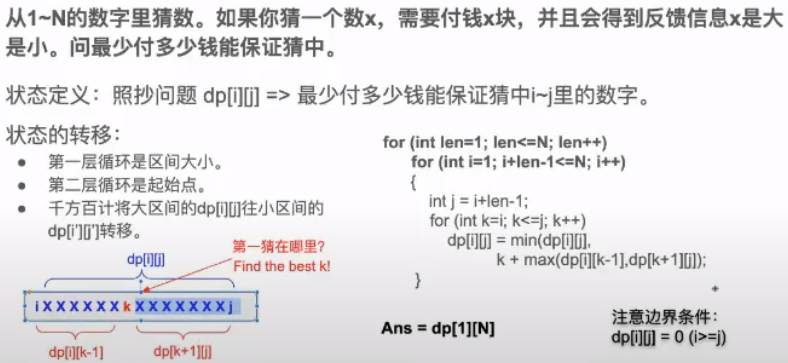
\includegraphics[width=.9\linewidth]{./pic/guessNumber.png}

\begin{minted}[frame=lines,fontsize=\scriptsize,linenos=false]{java}
private int dfs(int l, int r) {
    if (dp[l][r] > 0) return dp[l][r];
    if (l == r) return dp[l][r] = 0;
    if (l == r-1) return dp[l][r] = Math.min(l, r);
    int min = Integer.MAX_VALUE;
    for (int i = l; i <= r; i++) 
        min = Math.min(min, i + Math.max((i == r ? i : dfs(i+1, r)), (i == l ? i : dfs(l, i-1))));
    return dp[l][r] = min;
}
int [][] dp;
public int getMoneyAmount(int n) {
    dp = new int[n+1][n+1];
    return dfs(1, n);
}
\end{minted}
\section{1478. Allocate Mailboxes - Hard}
\label{sec-2-37}
Given the array houses and an integer k. where houses[i] is the location of the ith house along a street, your task is to allocate k mailboxes in the street.

Return the minimum total distance between each house and its nearest mailbox.

The answer is guaranteed to fit in a 32-bit signed integer.

解题思路分析:

对于如何安排邮箱位置,看到很多文章说应放在中位数的位置上,比如一共有1,2,3,4这4间房屋,不论房屋间的距离是多少,如果只有一个邮箱的话,放在房间2处(3也可以)最为合理。这个说法虽然正确,但实际上并不恰当。我们简单的讨论一下这个问题:
\begin{minted}[frame=lines,fontsize=\scriptsize,linenos=false]{java}
1.当只有1栋房屋,1个邮箱时,显然将邮箱放在房屋处最为合理,这时邮箱与房屋的距离为0。
2.当有2栋房屋,1个邮箱时,比如房屋1在坐标0处,房屋2在坐标10处,此时如果将邮箱放在坐标0的话,它与两栋房屋的距离和为10。
  放在坐标10的情况下距离和也为10。另外我们可以看出,不论邮箱放在两栋房屋之间的任意位置上,它与房屋的距离和都是10。因此
  通过此例可得出,中位数的说法虽然正确,但并不全面,不过这不影响本题解题,对于本题,我们统一将邮箱安排在房屋位置上是为
  了方便计算,因此才得出中位数的说法(本例房屋1和2都可以看做是中位数)。
3.当有3栋房屋,1个邮箱时,此时通过上面的例子可知,对于两侧的房子,将邮筒放在他们之间的任何位置对于结果没有任何影响,距
  离和都是两栋房子间的距离。但邮箱的位置会对中间的房子产生影响,因此,将其放置在中间房子的坐标上最为合理,这样邮箱与中
  间房屋的距离为0,可使得全局总距离最小。而中间的房屋正是3个房屋的中位数。
4.当有4栋房屋,1个邮箱时,与上例同理,对于两侧的房子,将邮筒放在他们之间的任何位置对于结果没有任何影响,因此邮箱可以考
  虑放在中间两个房屋的任何一个位置上。另外对于中间两个房屋,不论邮箱放置在其任何一个位置上,对于总距离都不会产生影响
 (这相当于第2条)。
\end{minted}

因此我们可以得出结论,当有N栋房屋,1个邮箱时,我们将邮箱放在房屋下标的中位数上最为合理。那么,如果有多个邮箱时该怎么办?其实也不难,本题最终可以理解为,我们将一个房屋数组分割为K个子数组(k为邮筒个数),每一个子数组中放置一个邮筒,求最优分割方式。这就变为了经典的动态规划DP问题,对于DP问题我习惯采用递归加记忆数组的方式,本题我们也采用递归方式讲解。

首先建立一个递归函数,参数为当前子区间开始位置index,以及剩余未分配邮筒个数k。起始时,子区间开始位置为下标0,邮筒个数为题目给定的整数k。递归时,当前子区间的开始坐标是参数index,结束坐标范围理论上可以是当前index到数组末尾为止,不过这里有一处可以优化,即要保证剩下的k-1个邮筒都能分配出去的话,还需要至少k-1个子区间,也就是说除了当前子区间外还至少需要k-1个房屋,因此当前子区间的结束坐标范围应该是当前index到length-k为止。我们从index循环至length-k,分别作为当前子区间的结束位置end。并通过中位数方式求出当前子区间[index, end]放置邮筒后的距离和(后文会给出方法)。然后将end加一作为下一个子区间的开始位置,同时k值减去一作为参数传入递归子问题中继续求解。递归函数的返回值加上当前子区间的距离和即是选择当前子区间范围后的一个结果sum。循环完所有当前子区间的结束位置end之后,所有sum中的最小值即是最优方案,也是本层递归的返回值。

接下来再为递归加上一个记忆数组。记忆数组相当于动态规划中使用到的DP数组。由于递归函数中存在2个变量,因此我们需要使用一个2维数组来描述该递归函数,并记录它的返回值。

最后,上文中提到需要求解子区间内放置一个邮筒后所有房屋与邮筒的距离和。这个问题没有太好的方式,只能暴力累加每个房屋与中位数房屋所在位置的距离。为了提高效率,我们可以事先计算好所有区间(排列组合)内放置一个邮筒时的距离和,方便递归中使用,也避免重复运算。这里可能有人会提出质疑,既然递归方法中已经使用了记忆数组,目的就是防止重复计算,这里为什么还担心重复计算距离和呢?原因很简单,记忆数组是二维数组,即在两个条件都满足的情况下才会使用记忆数组中的数据,比如我们计算过以下标5作为子区间起点,并且当前还剩2个油桶的递归函数返回值为x,即memo\footnote{DEFINITION NOT FOUND.}\textsuperscript{,}\,\footnote{DEFINITION NOT FOUND.}=x,再次遇到相同问题时我们可以直接返回x。但是遇到memo\footnotemark[4]{}\textsuperscript{,}\,\footnotemark[3]{}或者memo\footnotemark[4]{}\textsuperscript{,}\,\footnotemark[1]{}时,我们尚未做出过计算,同样还会进入到递归函数内部,如果没有事前计算好下标5到end(end取值范围是5到length-k)的距离和的话,还要重复计算一遍。

对于上述问题,还有一个更好的优化方式即再建立一个保存距离和的记忆数组,计算一个距离和记录一个,方便下次使用。

\begin{minted}[frame=lines,fontsize=\scriptsize,linenos=false]{java}
private int getDist(int [] arr, int i, int j) { // 求区间start到end间放置邮筒后的距离和 i: left, j: right
    if (dist[i][j] > 0) return dist[i][j];
    int m = i + (j-i)/2, v = arr[m], sum = 0;
    for (int k = i; k <= j; k++) 
        sum += Math.abs(arr[k] - v);
    return dist[i][j] = sum;
}
private int dfs(int [] arr, int idx, int k) {  // idx: 待分割大子区间的起始坐标;k: 待分割成的子区间的个数 
    if (idx == n || idx == n-k) return 0;
    if (dp[idx][k] > 0) return dp[idx][k];
    if (k == 1) return dp[idx][k] = getDist(arr, idx, n-1);
    int res = Integer.MAX_VALUE;
    for (int i = idx; i < n-(k-1); i++) 
        res = Math.min(res, getDist(arr, idx, i) + dfs(arr, i+1, k-1));
    return dp[idx][k] = res;
}
int [][] dp;
int [][] dist; // 这也是一种记忆数组优化
int n;
public int minDistance(int [] houses, int k) {
    n = houses.length;
    dist = new int [n][n];
    dp = new int [n][k+1];
    Arrays.sort(houses);
    return dfs(houses, 0, k);
}
\end{minted}

\section{486. Predict the Winner}
\label{sec-2-38}
You are given an integer array nums. Two players are playing a game with this array: player 1 and player 2.
Player 1 and player 2 take turns, with player 1 starting first. Both players start the game with a score of 0. At each turn, the player takes one of the numbers from either end of the array (i.e., nums\footnotemark[2]{} or nums[nums.length - 1]) which reduces the size of the array by 1. The player adds the chosen number to their score. The game ends when there are no more elements in the array.
Return true if Player 1 can win the game. If the scores of both players are equal, then player 1 is still the winner, and you should also return true. You may assume that both players are playing optimally.

博弈类题目,使用minMax思想,使自己分数最大化,对手分数尽量小,递归自顶向下求解。

该题不使用备忘机制同样能通过测试例,只不过耗时相对较长,单纯的比较取数后两players的分数差即可:Math.max(nums[l] - getScore(nums, l + 1, r), nums[r] - getScore(nums, l, r - 1));

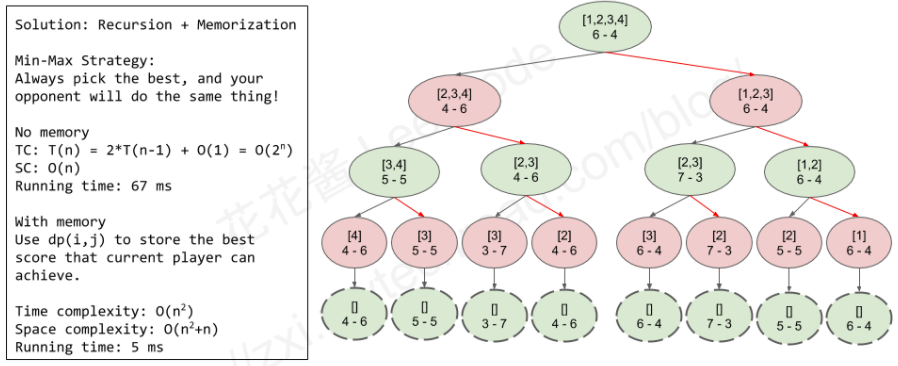
\includegraphics[width=.9\linewidth]{./pic/predictWinner.png}

\begin{minted}[frame=lines,fontsize=\scriptsize,linenos=false]{java}
private int helper( int [] arr, int i, int j) {
    if (i == j) return arr[i];
    else return Math.max(arr[i] - helper(arr, i+1, j), arr[j] - helper(arr, i, j-1));
}
public boolean PredictTheWinner(int[] nums) {
    int n = nums.length;
    if (n == 1) return true;
    return helper(nums, 0, n-1) >= 0;
}
\end{minted}

\section{877. Stone Game}
\label{sec-2-39}
Alice and Bob play a game with piles of stones. There are an even number of piles arranged in a row, and each pile has a positive integer number of stones piles[i].
The objective of the game is to end with the most stones. The total number of stones across all the piles is odd, so there are no ties.
Alice and Bob take turns, with Alice starting first. Each turn, a player takes the entire pile of stones either from the beginning or from the end of the row. This continues until there are no more piles left, at which point the person with the most stones wins.
Assuming Alice and Bob play optimally, return true if Alice wins the game, or false if Bob wins.
\begin{minted}[frame=lines,fontsize=\scriptsize,linenos=false]{java}
// 使用helper函数表示Alex能比Lee多选的分数。可能比双函数更简洁易懂了。
// 记忆化递归的缺点:1.有可能爆栈;2.无法降维,而DP是可以降维的。
// 模板:
// dfs + memoization模板
private int dfs(int [] arr, int l, int r) {
    if (l > r) return 0;
    if (dp[l][r] > 0) return dp[l][r]; // 走了来时的路,不需要重走,直接返回
    dp[l][r] = Math.max(arr[l] - dfs(arr, l+1, r), arr[r]-dfs(arr, l, r-1));
    return dp[l][r];
}
int [][] dp; 
public boolean stoneGame(int[] piles) {
    int n = piles.length;
    dp = new int[n][n];
    return dfs(piles, 0, n-1) > 0;
}
// 动态规划解法比较难想,dp数组的第i个位置表示的是从第i个石头到第i+l-1个石头之间最大的比对手得分。
// 使用的是一个长度变量和起始索引,计算每个位置开始的长度1~N长度的区间的dp状态。
public boolean stoneGame(int[] piles) {
    int n = piles.length;
    int [][] dp = new int[n][n];
    for (int i = n-1; i >= 0; i--) { // 最后一列
        dp[i][i] = piles[i];         // 填右上角
        for (int j = i+1; j < n; j++) 
            dp[i][j] = Math.max(piles[i] - dp[i+1][j], piles[j]-dp[i][j-1]);

    }
    return dp[0][n-1] > 0;
}
\end{minted}
\section{1140. Stone Game II}
\label{sec-2-40}
Alice and Bob continue their games with piles of stones.  There are a number of piles arranged in a row, and each pile has a positive integer number of stones piles[i].  The objective of the game is to end with the most stones. 
Alice and Bob take turns, with Alice starting first.  Initially, M = 1.
On each player's turn, that player can take all the stones in the first X remaining piles, where 1 <= X <= 2M.  Then, we set M = max(M, X).
The game continues until all the stones have been taken.
Assuming Alice and Bob play optimally, return the maximum number of stones Alice can get.
\begin{minted}[frame=lines,fontsize=\scriptsize,linenos=false]{java}
// dfs + memoization模板
// 当次取的最优策略是限制下一次取的数量
private int dfs(int [] arr, int idx, int m) {
    if (dp[idx][m] > 0) return dp[idx][m];
    if (idx == n) return 0;
    if (idx >= n - 2 * m) {
        dp[idx][m] = suf[idx];
        return dp[idx][m];
    }
    int min = Integer.MAX_VALUE;
    for (int i = 1; i <= 2 * m; i++) // 选择限制对手得分最少的情况
        min = Math.min(min, dfs(arr, idx+i, Math.max(m, i))); 
    dp[idx][m] = suf[idx] - min;
    return dp[idx][m];
}
int [][] dp; 
int [] suf;
int n;
public int stoneGameII(int[] piles) {
    n = piles.length;
    dp = new int [n][2*n];
    suf = new int [n+1];
    for (int i = n-1; i >= 0; i--) 
        suf[i] = suf[i+1] + piles[i];
    return dfs(piles, 0, 1);
}
\end{minted}
\section{1872. Stone Game VIII}
\label{sec-2-41}
Alice and Bob take turns playing a game, with Alice starting first.
There are n stones arranged in a row. On each player's turn, while the number of stones is more than one, they will do the following:
Choose an integer x > 1, and remove the leftmost x stones from the row.
Add the sum of the removed stones' values to the player's score.
Place a new stone, whose value is equal to that sum, on the left side of the row.
The game stops when only one stone is left in the row.
The score difference between Alice and Bob is (Alice's score - Bob's score). Alice's goal is to maximize the score difference, and Bob's goal is the minimize the score difference.
Given an integer array stones of length n where stones[i] represents the value of the ith stone from the left, return the score difference between Alice and Bob if they both play optimally.
\begin{minted}[frame=lines,fontsize=\scriptsize,linenos=false]{java}
// 使用 dp(i) 表示还剩下 [i, n) 要选择的情况下,Alice 所能得到的最大分数差。
//     对于某个玩家来说,其对应决策可以分为两种:
//     选取当前数及之前的所有数(等价于 pres[pos],其中 pos 为上个玩家选完后的下个位置),那么 dp[i] = pres[i] - dp[i+1]。
//     这是因为 bob 也会最大化发挥。
//     不选择当前数(可能选下一个,下下一个。。。 etc),那么 dp[i] = dp[i + 1]
public int stoneGameVIII(int[] stones) {
    int n = stones.length;
    int [] dp = new int [n];
    Arrays.fill(dp, Integer.MIN_VALUE);
    int [] pre = new int [n+1];
    for (int i = 1; i <= n; i++)
        pre[i] = pre[i-1] + stones[i-1];
    dp[n-1] = pre[n];
    for (int i = n-2; i >= 0; i--) 
        dp[i] = Math.max(dp[i+1], pre[i+1]-dp[i+1]);
    return dp[1];
}
\end{minted}

\section{123. Best Time to Buy and Sell Stock III}
\label{sec-2-42}
You are given an array prices where prices[i] is the price of a given stock on the ith day.
Find the maximum profit you can achieve. You may complete at most two transactions.
Note: You may not engage in multiple transactions simultaneously (i.e., you must sell the stock before you buy again).
\begin{minted}[frame=lines,fontsize=\scriptsize,linenos=false]{java}
// k 次交易 = k 个 non-overlapping subarray
//     以这个角度去想,无非就是从两个方向扫描,
//     利用 localMin / localMax 与当前元素的差值,去构造从左边/右边扫的 dp 数组。
//     left[i] : 从最左面到 i 所能获得的最大利益(单次交易)
//     right[i] : 从 i 到最右面所能获得的最大利益(单次交易)
public int maxProfit(int[] prices) {
    int n = prices.length;
    int [] left = new int [n];
    int [] right = new int[n];
    int locMin = prices[0];
    int globalMax = Integer.MIN_VALUE;
    for (int i = 1; i < n; i++) {
        globalMax = Math.max(globalMax, Math.max(0, prices[i] - locMin));
        locMin = Math.min(locMin, prices[i]);
        left[i] = globalMax;
    }
    int locMax = prices[n-1];
    globalMax = Integer.MIN_VALUE;
    for (int i = n-2; i >= 0; i--) {
        globalMax = Math.max(globalMax, Math.max(0, locMax - prices[i]));
        locMax = Math.max(locMax, prices[i]);
        right[i] = globalMax;
    }
    globalMax = 0;
    for (int i = 0; i < n-1; i++) 
        globalMax = Math.max(globalMax, left[i] + right[i+1]);
    globalMax = Math.max(globalMax, left[n-1]);
    return globalMax;
}
\end{minted}

\section{188. Best Time to Buy and Sell Stock IV}
\label{sec-2-43}
You are given an integer array prices where prices[i] is the price of a given stock on the ith day, and an integer k.
Find the maximum profit you can achieve. You may complete at most k transactions.
Note: You may not engage in multiple transactions simultaneously (i.e., you must sell the stock before you buy again).
\begin{minted}[frame=lines,fontsize=\scriptsize,linenos=false]{java}
public int maxProfit(int k, int [] prices) {
    if (prices == null || prices.length == 0) return 0;
    int n = prices.length;
    int diff = 0;
    if (k >= n/2) {
        int res = 0;
        for (int i = 1; i < n; i++) {
           diff = prices[i] - prices[i-1];
            if (diff > 0) res += diff;
        }
        return res;
    }
    int [][] locMax = new int [n][k+1];
    int [][] gloMax = new int [n][k+1];
    for (int i = 1; i < n; i++) {
        diff = prices[i] - prices[i-1];
        for (int j = 1; j <= k && j * 2 <= i+1; j++) {
            locMax[i][j] = Math.max(locMax[i-1][j], gloMax[i-1][j-1]) + diff;
            gloMax[i][j] = Math.max(locMax[i][j], gloMax[i-1][j]);
        }
    }
    return gloMax[n-1][k];
}
\end{minted}

\section{714. Best Time to Buy and Sell Stock with Transaction Fee}
\label{sec-2-44}
You are given an array prices where prices[i] is the price of a given stock on the ith day, and an integer fee representing a transaction fee.
Find the maximum profit you can achieve. You may complete as many transactions as you like, but you need to pay the transaction fee for each transaction.
Note: You may not engage in multiple transactions simultaneously (i.e., you must sell the stock before you buy again).
\begin{minted}[frame=lines,fontsize=\scriptsize,linenos=false]{java}
public int maxProfit(int[] prices, int fee) {
    int n = prices.length;
    int [] sold = new int[n];
    int [] hold = new int[n];
    hold[0] = -prices[0];
    for (int i = 1; i < n; i++) {
        sold[i] = Math.max(sold[i-1], hold[i-1]+prices[i]-fee);
        hold[i] = Math.max(hold[i-1], sold[i-1]-prices[i]);
    }
    return sold[n-1];
}
\end{minted}

\section{309. Best Time to Buy and Sell Stock with Cooldown}
\label{sec-2-45}
You are given an array prices where prices[i] is the price of a given stock on the ith day.
Find the maximum profit you can achieve. You may complete as many transactions as you like (i.e., buy one and sell one share of the stock multiple times) with the following restrictions:
After you sell your stock, you cannot buy stock on the next day (i.e., cooldown one day).
Note: You may not engage in multiple transactions simultaneously (i.e., you must sell the stock before you buy again).
\begin{itemize}
\item 感觉自己DP的能力还是太弱,越是这样越需要迎难而上。
\item 这个题和714. Best Time to Buy and Sell Stock with Transaction Fee比较像。做题方法都是使用了两个数组:
\item cash 该天结束手里没有股票的情况下,已经获得的最大收益
\item hold 该天结束手里有股票的情况下,已经获得的最大收益
\item 状态转移方程式这样的:
\begin{itemize}
\item cash[i]代表的是手里没有股票的收益,这种可能性是今天卖了或者啥也没干。max(昨天手里有股票的收益+今天卖股票的收益,昨天手里没有股票的收益), 即max(sell[i - 1], hold[i - 1] + prices[i]);
\item hold[i]代表的是手里有股票的收益,这种可能性是今天买了股票或者啥也没干,今天买股票必须昨天休息。所以为max(今天买股票是前天卖掉股票的收益-今天股票的价格,昨天手里有股票的收益)。即max(hold[i - 1], sell[i - 2] - prices[i])。
\end{itemize}
\item 另外需要注意的是,题目说的是昨天卖了股票的话今天不能买,对于开始的第一天,不可能有卖股票的行为,所以需要做个判断。
\item 该算法的时间复杂度是O(n),空间复杂度是O(n)。
\end{itemize}
\begin{minted}[frame=lines,fontsize=\scriptsize,linenos=false]{java}
public int maxProfit(int[] prices) {
    int n = prices.length;
    int [] sold = new int [n];
    int [] hold = new int [n];
    hold[0] = -prices[0];
    for (int i = 1; i < n; i++) {   // ith: do nothing, selling hold[i-1]
        sold[i] = Math.max((i >= 2 ? sold[i-1] : 0), hold[i-1] + prices[i]); // 今天卖了股票,或者今天什么也没有干
        hold[i] = Math.max(hold[i-1], (i >= 2 ? sold[i-2] : 0) - prices[i]); // 今天买了股票,或者今天什么也没有干
    }
    return Math.max(sold[n-1], hold[n-1]);
}
\end{minted}

\section{673. Number of Longest Increasing Subsequence}
\label{sec-2-46}
Given an integer array nums, return the number of longest increasing subsequences.
Notice that the sequence has to be strictly increasing.
\begin{minted}[frame=lines,fontsize=\scriptsize,linenos=false]{java}
public int findNumberOfLIS(int[] nums) { // dynamic programming
    int n = nums.length;
    int [][] arr = new int[n][2];
    int maxLength = 1;
    for (int i = 0; i < n; i++) 
        Arrays.fill(arr[i], 1);
    for (int i = 0; i < n; i++) {
        for (int j = i+1; j < n; j++) {
            if (nums[j] > nums[i]) {
                if (arr[i][0] + 1 > arr[j][0]) {
                    arr[j][0] = arr[i][0] +1;
                    arr[j][1] = arr[i][1];
                    maxLength = Math.max(maxLength, arr[j][0]);
                } else if (arr[i][0] + 1 == arr[j][0])
                    arr[j][1] += arr[i][1];
            }
         }
    }
    int cnt = 0;
    for (int i = 0; i < n; i++) 
        if (arr[i][0] == maxLength) cnt += arr[i][1];
    return cnt;
}
\end{minted}

\section{1896. Minimum Cost to Change the Final Value of Expression - Hard}
\label{sec-2-47}
You are given a valid boolean expression as a string expression consisting of the characters '1','0','\&' (bitwise AND operator),'|' (bitwise OR operator),'(', and ')'.

For example, "()1|1" and "(1)\&()" are not valid while "1", "(((1))|(0))", and "1|(0\&(1))" are valid expressions.
Return the minimum cost to change the final value of the expression.

For example, if expression = "1|1|(0\&0)\&1", its value is 1|1|(0\&0)\&1 = 1|1|0\&1 = 1|0\&1 = 1\&1 = 1. We want to apply operations so that the new expression evaluates to 0.
The cost of changing the final value of an expression is the number of operations performed on the expression. The types of operations are described as follows:

Turn a '1' into a '0'.
Turn a '0' into a '1'.
Turn a '\&' into a '|'.
Turn a '|' into a '\&'.
Note: '\&' does not take precedence over '|' in the order of calculation. Evaluate parentheses first, then in left-to-right order.
\begin{minted}[frame=lines,fontsize=\scriptsize,linenos=false]{java}
private int [] getMinOperations(int va, int vb, int ca, int cb, char sign) {
    if (sign == '&') {
        if (va == 1 && vb == 1)      // 1&1, 将其中一个1反转为0
            return new int [] {1, Math.min(ca, cb)};
        else if (va == 0 && vb == 0) // 0&0, 将其中一个0反转为1,并将&反转为|
            return new int [] {0, Math.min(ca, cb) + 1};
        else return new int [] {0, 1}; // 1&0, 将&反转为|
    } else {
        if (va == 1 && vb == 1)        // 1|1,将其中一个1反转为0,并将|反转为&
            return new int [] {1, Math.min(ca, cb) + 1};
        else if (va == 0 && vb == 0)   // 0|0,将其中一个0反转为1
            return new int [] {0, Math.min(ca, cb)};
        else return new int [] {1, 1}; // 1|0,将|反转为&
    }
}
public int minOperationsToFlip(String expression) {
    Stack<Integer> res = new Stack<>();
    Stack<Character> sgn = new Stack<>();
    Stack<Integer> cnt = new Stack<>();
    for (char c : expression.toCharArray()) {
        if (c == '(' || c == '&' || c == '|') {
            sgn.push(c);
            continue;
        } else if (c == ')') sgn.pop();
        else {
            res.push((int)(c - '0'));
            cnt.push(1);
        }
        if (res.size() > 1 && sgn.peek() != '(') {
            int [] loc = getMinOperations(res.pop(), res.pop(), cnt.pop(), cnt.pop(), sgn.pop());
            res.push(loc[0]); // expr results
            cnt.push(loc[1]); // min operations
        }
    }
    return cnt.peek();
}
\end{minted}

\section{823. Binary Trees With Factors}
\label{sec-2-48}
Given an array of unique integers, arr, where each integer arr[i] is strictly greater than 1.
We make a binary tree using these integers, and each number may be used for any number of times. Each non-leaf node's value should be equal to the product of the values of its children.
Return the number of binary trees we can make. The answer may be too large so return the answer modulo 109 + 7.
\begin{minted}[frame=lines,fontsize=\scriptsize,linenos=false]{java}
public int numFactoredBinaryTrees(int[] arr) {
    int n = arr.length;
    Arrays.sort(arr);
    Map<Integer, Long> dp = new HashMap<>();
    int mod = 1_000_000_007;
    long res = 0;
    long max = 0;
    for (int i = 0; i < n; i++) {
        dp.put(arr[i], 1l);
        for (int j = 0; j < i; j++) {
            if (arr[i] % arr[j] == 0 && dp.containsKey(arr[i]/arr[j])) {
                max = dp.get(arr[i]) + dp.get(arr[j]) * dp.get(arr[i]/arr[j]);
                dp.put(arr[i], max % mod);
            }
        }
        res += dp.get(arr[i]);
        res %= mod;
    }
    return (int)(res % mod);
}
\end{minted}

\section{907. Sum of Subarray Minimums}
\label{sec-2-49}
Given an array of integers arr, find the sum of min(b), where b ranges over every (contiguous) subarray of arr. Since the answer may be large, return the answer modulo 109 + 7.
\begin{minted}[frame=lines,fontsize=\scriptsize,linenos=false]{java}
public int sumSubarrayMins(int[] arr) {
    int n = arr.length;
    // for each A[i], find k <= i <= j, so that A[i] is the min from [k,j]
    // sum += A[i] * (i-k+1) * (j-i+1)
    // so we need to find the next min to the right and to the left
    //这个过程可以简化为使用一个栈。对于被某个数从栈中弹出的数而言,它右侧第一个比它小的数就是这个数。所以我们可以对所有被弹出的数得到左侧的区间范围和右侧的区间范围。我觉得这是一种非常聪明的做法。 这个栈我看得稀里糊涂,再想一下
    long [] right = new long [n];  // next smaller element index to the right 
    long [] left = new long[n];    // next smaller element index to the left
    Stack<Integer> s = new Stack<>();
    for (int i = 0; i < n; i++) {
        while (!s.isEmpty() && arr[i] <= arr[s.peek()]) {
            right[s.pop()] = i-1;
        }
        s.push(i);
    }
    while (!s.isEmpty()) {
        right[s.pop()] = n-1;
    }
    s.clear();
    for (int i = n-1; i >= 0; i--) {
        while (!s.isEmpty() && arr[i] < arr[s.peek()])
            left[s.pop()] = i+1;
        s.push(i);
    }
    while (!s.isEmpty())
        left[s.pop()] = 0;
    long sum = 0;
    long leftsize = 0, rightsize = 0;
    for (int i = 0; i < n; i++) {
        leftsize = i - left[i] +1;
        rightsize = right[i] - i + 1;
        sum += arr[i] * leftsize * rightsize;
        sum %= mod;
    }
    return (int)sum;
}
int mod = 1_000_000_007;
public int sumSubarrayMins(int[] arr) {
    int n = arr.length;
    long [] left = new long[n];
    long [] right = new long[n];
    long sum = 0;
    long cnt = 0;
    int j = 0;
    for (int i = 0; i < n; i++) { // 计算左边比自身大的数的个数
        cnt = 1;
        j = i-1;
        while (j >= 0 && arr[j] >= arr[i]) {
            cnt += left[j];
            j -= left[j];
        }
        left[i] = cnt;
    }
    // 就是因为计算了两个方向,所以对于数组里面有相同元素的情况下,需要特别考虑一下。
    //     不能重复计算, 也不能漏掉,
    //     具体就是一个方向的时候用<=, 另外一个方向的时候用<。 这个在做的时候也bug了。
    for (int i = n-1; i >= 0; i--) { // 计算右边比自身大的数的个数
        cnt = 1;
        j = i+1;
        while (j < n && arr[j] > arr[i]) {
            cnt += right[j];
            j += right[j];
        }
        right [i] = cnt;
    }
    for (int i = 0; i < n; i++) 
        sum += arr[i] * left[i] * right[i];
    return (int) (sum % mod);
}
\end{minted}

\section{494. Target Sum - Medium}
\label{sec-2-50}
You are given an integer array nums and an integer target.

You want to build an expression out of nums by adding one of the symbols '+' and '-' before each integer in nums and then concatenate all the integers.

For example, if nums = [2, 1], you can add a '+' before 2 and a '-' before 1 and concatenate them to build the expression "+2-1".
Return the number of different expressions that you can build, which evaluates to target.
\begin{itemize}
\item 该题是一道非常经典的题目,在面试中很可能会考到。该题有多种解法。
\item 第一种解法:DFS,brute force。我们对nums数组中的每个数字,都尝试在其前面添加正号和负号,最后暴力求解,统计数组中各数字组合值为target的情况。(该理解是错误的,我们可以使用带备忘录机制的自顶向下的DP方法,代码见下)
\end{itemize}
\begin{minted}[frame=lines,fontsize=\scriptsize,linenos=false]{java}
//带备忘录机制的自顶向下DP解法 //map存储重复的值,there are obvious a lot of overlap subproblems
private int helper(int[] nums, int index, int sum, int S, Map<String, Integer> map){ 
    String encodeString = index + "->" + sum; //经过之前不同的运算过程到达index的sum值碰巧与之前某一个运算过程的结果相同
    if (map.containsKey(encodeString)) return map.get(encodeString);
    if (index == nums.length)
        if (sum == S) return 1;
        else return 0;
    int curNum = nums[index];
    int add = helper(nums, index + 1, sum - curNum, S, map);
    int minus = helper(nums, index + 1, sum + curNum, S, map);
    map.put(encodeString, add + minus);
    return add + minus;
}
public int findTargetSumWays(int[] nums, int S) {
    if (nums == null || nums.length == 0) return 0;
    return helper(nums, 0, 0, S, new HashMap<>());
}
\end{minted}
\begin{itemize}
\item 第二种解法:DP。我们使用Vi来表示数组中的前i个数所能求得的和的集合。初始化时
\end{itemize}
\begin{minted}[frame=lines,fontsize=\scriptsize,linenos=false]{java}
V0 = {0}     //表示前0个数的和为0
Vi = {V(i-1) + ai} U {V(i-1) - ai}
\end{minted}

Vn就是nums数组所有数字的组合值之和的集合

根据上面的思路,我们知道数组中数字若全为正号其和为sum,全为负号其和为-sum。若不选数组中任何一个数,则和为0。因此,我们设立一个长度为2*sum+1的数组ways,ways[i]表示我们选择前m个数,其和可能为i的情况数,m = 0,1,\ldots{}nums.length。可参考下图

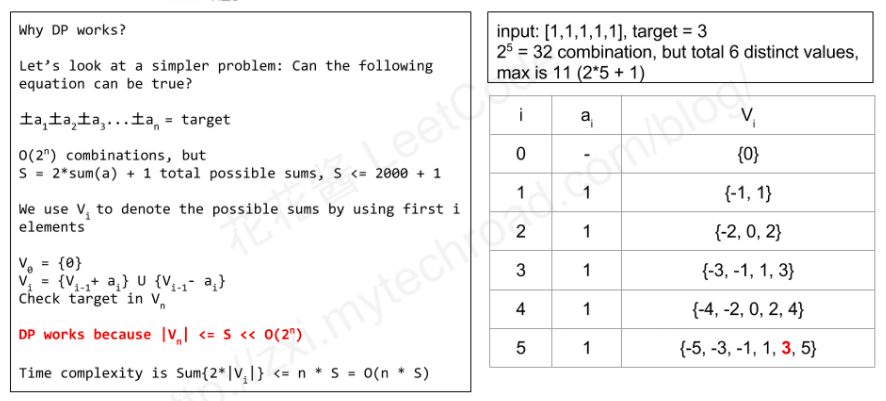
\includegraphics[width=.9\linewidth]{./pic/targetSum.png}

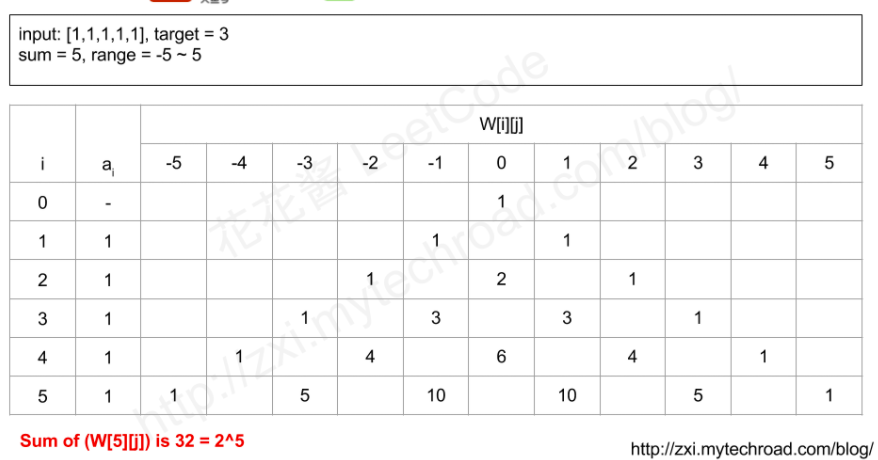
\includegraphics[width=.9\linewidth]{./pic/targetSum2.png}

\section{1477. Find Two Non-overlapping Sub-arrays Each With Target Sum}
\label{sec-2-51}
Given an array of integers arr and an integer target.
You have to find two non-overlapping sub-arrays of arr each with a sum equal target. There can be multiple answers so you have to find an answer where the sum of the lengths of the two sub-arrays is minimum.
Return the minimum sum of the lengths of the two required sub-arrays, or return -1 if you cannot find such two sub-arrays.
\begin{minted}[frame=lines,fontsize=\scriptsize,linenos=false]{java}
// 找出数组中等于target的最小非重叠区间的长度,用dp[i]表示当前i以及i之前的满足条件的最小区间长度,状态更新规则为
//     dp[i]=min(dp[i-1],i-j+1) if sum[j,i]=target
//     答案更新规则
//     res=min(res,dp[j−1]+i−j+1)
public int minSumOfLengths(int[] arr, int target) {
    int n = arr.length;
    int [] dp = new int [n];
    Arrays.fill(dp, Integer.MAX_VALUE);
    int cur = 0, s = 0;
    int res = Integer.MAX_VALUE, minLen = Integer.MAX_VALUE;
    for (int i = 0; i < n; i++) {
        cur += arr[i];
        while (cur > target) {
            cur -= arr[s];
            s += 1;
        }
        if (cur == target) {
            int curLen = i - s + 1;
            if (s > 0 && dp[s-1] != Integer.MAX_VALUE) 
                res = Math.min(res, curLen + dp[s-1]);
            minLen = Math.min(minLen, curLen);
        }
        dp[i] = minLen;
    }
    return res == Integer.MAX_VALUE ? -1 : res;
}
\end{minted}

\section{1771. Maximize Palindrome Length From Subsequences}
\label{sec-2-52}
You are given two strings, word1 and word2. You want to construct a string in the following manner:
Choose some non-empty subsequence subsequence1 from word1.
Choose some non-empty subsequence subsequence2 from word2.
Concatenate the subsequences: subsequence1 + subsequence2, to make the string.
Return the length of the longest palindrome that can be constructed in the described manner. If no palindromes can be constructed, return 0.
A subsequence of a string s is a string that can be made by deleting some (possibly none) characters from s without changing the order of the remaining characters.
A palindrome is a string that reads the same forward as well as backward.
\begin{minted}[frame=lines,fontsize=\scriptsize,linenos=false]{java}
public int longestPalindrome(String s, String t) { // 这个题目没有懂,需要再好好看一下
    int m = s.length();
    int n = t.length();
    int mn = m + n;
    String st = s + t;
    int [][] dp = new int [mn][mn];
    for (int i = 0; i < mn; i++)
        dp[i][i] = 1;
    for (int l = 2; l <= mn; l++) {
        for (int i = 0, j = i+l-1; j < mn; i++,j++) { // 
            if (st.charAt(i) == st.charAt(j))
                dp[i][j] = dp[i+1][j-1] + 2;
            else dp[i][j] = Math.max(dp[i+1][j], dp[i][j-1]);                         
        }
    }
    int ans = 0;
    for (int i = 0; i < m; i++) {
        for (int j = 0; j < n; j++) {
            if (s.charAt(i) == t.charAt(j))
                ans = Math.max(ans, dp[i][m+j]); // 
        }
    }
    return ans;
}
\end{minted}

\section{907. Sum of Subarray Minimums}
\label{sec-2-53}
Given an array of integers arr, find the sum of min(b), where b ranges over every (contiguous) subarray of arr. Since the answer may be large, return the answer modulo 109 + 7.
\begin{minted}[frame=lines,fontsize=\scriptsize,linenos=false]{java}
        public int sumSubarrayMins(int[] arr) {
            int n = arr.length;
            // for each A[i], find k <= i <= j, so that A[i] is the min from [k,j]
            // sum += A[i] * (i-k+1) * (j-i+1)
            // so we need to find the next min to the right and to the left
            //这个过程可以简化为使用一个栈。对于被某个数从栈中弹出的数而言,它右侧第一个比它小的数就是这个数。所以我们可以对所有被弹出的数得到左侧的区间范围和右侧的区间范围。我觉得这是一种非常聪明的做法。 这个栈我看得稀里糊涂,再想一下
            long [] right = new long [n];  // next smaller element index to the right 
            long [] left = new long[n];    // next smaller element index to the left
            Stack<Integer> s = new Stack<>();
            for (int i = 0; i < n; i++) {
                while (!s.isEmpty() && arr[i] <= arr[s.peek()]) {
                    right[s.pop()] = i-1;
                }
                s.push(i);
            }
            while (!s.isEmpty()) {
                right[s.pop()] = n-1;
            }
            s.clear();
            for (int i = n-1; i >= 0; i--) {
                while (!s.isEmpty() && arr[i] < arr[s.peek()])
                    left[s.pop()] = i+1;
                s.push(i);
            }
            while (!s.isEmpty())
                left[s.pop()] = 0;
            long sum = 0;
            long leftsize = 0, rightsize = 0;
            for (int i = 0; i < n; i++) {
                leftsize = i - left[i] +1;
                rightsize = right[i] - i + 1;
                sum += arr[i] * leftsize * rightsize;
                sum %= mod;
            }
            return (int)sum;
        }
        int mod = 1_000_000_007;
        public int sumSubarrayMins(int[] arr) {
            int n = arr.length;
            long [] left = new long[n];
            long [] right = new long[n];
            long sum = 0;
            long cnt = 0;
            int j = 0;
            for (int i = 0; i < n; i++) { // 计算左边比自身大的数的个数
                cnt = 1;
                j = i-1;
                while (j >= 0 && arr[j] >= arr[i]) {
                    cnt += left[j];
                    j -= left[j];
                }
                left[i] = cnt;
            }
            // 就是因为计算了两个方向,所以对于数组里面有相同元素的情况下,需要特别考虑一下。
            //     不能重复计算, 也不能漏掉,
            //     具体就是一个方向的时候用<=, 另外一个方向的时候用<。 这个在做的时候也bug了。
            for (int i = n-1; i >= 0; i--) { // 计算右边比自身大的数的个数
                cnt = 1;
                j = i+1;
                while (j < n && arr[j] > arr[i]) {
                    cnt += right[j];
                    j += right[j];
                }
                right [i] = cnt;
            }
            for (int i = 0; i < n; i++) 
                sum += arr[i] * left[i] * right[i];
            return (int) (sum % mod);
        }
\end{minted}

\section{689. Maximum Sum of 3 Non-Overlapping Subarrays}
\label{sec-2-54}
Given an integer array nums and an integer k, find three non-overlapping subarrays of length k with maximum sum and return them.
Return the result as a list of indices representing the starting position of each interval (0-indexed). If there are multiple answers, return the lexicographically smallest one.
\begin{minted}[frame=lines,fontsize=\scriptsize,linenos=false]{java}
public int[] maxSumOfThreeSubarrays(int[] nums, int k) {
    int n = nums.length;
    int [] pre = new int [n+1];
    for (int i = 1; i <= n; i++) 
        pre[i] = pre[i-1] + nums[i-1];
    // left[i]表示在区间[0, i]范围内长度为k且和最大的子数组的起始位置
    // right[i]表示在区间[i, n - 1]范围内长度为k且和最大的子数组的起始位置
    int [] left = new int [n];
    int [] right = new int [n];
    int [] res = new int [3];
    Arrays.fill(right, n-k);
    for (int i = k, total = pre[k]-pre[0]; i < n; i++) {
        if (pre[i+1] - pre[i+1-k] > total) {
            left[i]= i+1-k;
            total = pre[i+1] - pre[i+1-k];
        } else left[i] = left[i-1];
    }
    for (int i = n-1-k, total = pre[n]-pre[n-k]; i >= 0; i--) {
        if (pre[i+k] - pre[i] >= total) {
            right[i] = i;
            total = pre[i+k] - pre[i];
        } else right[i] = right[i+1];
    }
    int max = Integer.MIN_VALUE;
    for (int i = k; i <= n-2*k; i++) {
        int l = left[i-1];
        int r = right[i+k];
        int total = (pre[i+k]-pre[i]) + (pre[k+l]-pre[l]) + (pre[r+k] - pre[r]);
        if (max < total) {
            max = total;
            res = new int [] {l, i, r};
        }
    }
    return res;
}
\end{minted}

\section{363. Max Sum of Rectangle No Larger Than K}
\label{sec-2-55}
Given an m x n matrix matrix and an integer k, return the max sum of a rectangle in the matrix such that its sum is no larger than k.
It is guaranteed that there will be a rectangle with a sum no larger than k.
\begin{minted}[frame=lines,fontsize=\scriptsize,linenos=false]{java}
public int maxSumSubmatrix(int[][] mat, int k) {
    int m = mat.length;
    int n = mat[0].length;
    if (m == 1 && n == 1) return mat[0][0];
    int [][] pre = new int [m][n];
    int res = Integer.MIN_VALUE;
    for (int i = 0; i < m; i++) {
        for (int j = 0; j < n; j++) {
            int t = mat[i][j];
            if (i > 0) t += pre[i-1][j];
            if (j > 0) t += pre[i][j-1];
            if (i > 0 && j > 0) t -= pre[i-1][j-1];
            pre[i][j] = t;
            for (int r = 0; r <= i; r++) {
                for (int c = 0; c <= j; c++) {
                    int d = pre[i][j];
                    if (r > 0) d -= pre[r-1][j];
                    if (c > 0) d -= pre[i][c-1];
                    if (r > 0 && c > 0) d += pre[r-1][c-1];
                    if (d <= k) res = Math.max(res, d);
                }
            }
        }
    }
    return res;
}
// 把二维数组按行或列拆成多个一维数组,然后利用一维数组的累加和来找符合要求的数字,
// 这里用了 lower_bound 来加快的搜索速度,也可以使用二分搜索法来替代。
public int maxSumSubmatrix(int[][] mat, int target) {
    int row = mat.length;
    int col = mat[0].length;
    int res = Integer.MIN_VALUE;
    boolean key = col > row ? false : true;
    int m = Math.min(row, col);
    int n = Math.max(row, col);
    int [] pre = new int [n];
    TreeSet<Integer> ts = new TreeSet<>(); //用来保存当前高度下,长度为从0开始到k位置的矩形的结果。理解set的含义是解决此题的关键。
    Integer tmp = 0;
    for (int i = 0; i < m; i++) { // 找从第i行开始一直到第0行这i+1行的可能组成的矩形长度
        Arrays.fill(pre, 0);
        for (int j = i; j >= 0; j--) {
            ts.clear();
            ts.add(0);
            int curSum = 0;
            for (int k = 0; k < n; k++) {
                if (key)
                    pre[k] += mat[k][j];
                else pre[k] += mat[j][k];
                curSum += pre[k];
                 // * 因为要满足  (sum-set中的元素)<=target,
                 // * 而且sum-set中的元素的值要尽可能的大,
                 // * 所以也就是再求小于等于sum-target中满足条件的元素的最小的一个
                 // * 正好TreeSet中提供了这个方法ceil(),可以很方便的找出这个元素
                tmp = ts.ceiling(curSum - target);
                if (tmp != null) res = Math.max(res, curSum - tmp);
                ts.add(curSum);
            }
        }
    }
    return res;
}
\end{minted}

\section{805. Split Array With Same Average}
\label{sec-2-56}
You are given an integer array nums.
You should move each element of nums into one of the two arrays A and B such that A and B are non-empty, and average(A) == average(B).
Return true if it is possible to achieve that and false otherwise.
Note that for an array arr, average(arr) is the sum of all the elements of arr over the length of arr.
\begin{minted}[frame=lines,fontsize=\scriptsize,linenos=false]{java}
public boolean splitArraySameAverage(int[] nums) {
    int n = nums.length;
    int m = n / 2;
    int sum = Arrays.stream(nums).sum();
    boolean poss = false;
    for (int i = 1; i <= m; i++) 
        if (sum * i % n == 0) {
            poss = true;
            break;
        }
    if (!poss) return false;
    List<Set<Integer>> ls = new ArrayList<>();
    for (int i = 0; i <= m; i++) 
        ls.add(new HashSet<Integer>());
    ls.get(0).add(0);    // 这种构建子序列和的方法,要学习一下
    for (int v : nums)  // for each element in A, we try to add it to sums[i] by joining sums[i - 1]
        for (int i = m; i >= 1; i--) 
            for (int t : ls.get(i-1)) 
                ls.get(i).add(t + v);
    for (int i = 1; i <= m; i++) {
        if (sum * i % n == 0 && ls.get(i).contains(sum * i / n))
            return true;
    }
    return false;
}
\end{minted}

\section{1981. Minimize the Difference Between Target and Chosen Elements}
\label{sec-2-57}
You are given an m x n integer matrix mat and an integer target.
Choose one integer from each row in the matrix such that the absolute difference between target and the sum of the chosen elements is minimized.
Return the minimum absolute difference.
The absolute difference between two numbers a and b is the absolute value of a - b.
\begin{minted}[frame=lines,fontsize=\scriptsize,linenos=false]{java}
// DP + BitSet : 这里面有个小问题需要挑出来
// 使用一个DP数组存下当前行和之前行每行选一个数可能构成的和,
// 在本题中,可以使用BitSet(简介)来存储之前行可以组成的和(由于所有数的最大值为70,而行数最大也为70,故BitSet最大的位数即为4900)。
// 对于当前行,遍历BitSet已经set过的位(即代表之前行可能组成的和),然后加上当前数,set新的和
// 最后遍历BitSet,求出当前位与target的最小值
public int minimizeTheDifference(int[][] mat, int target) {
    int m = mat.length;
    int n = mat[0].length;
    BitSet sum = new BitSet(); // 遍历每一行,存下当前行和之前行可能组成的和
    for (int i = 0; i < n; i++) // 初始时存下第一行
        sum.set(mat[0][i]);
    for (int i = 1; i < m; i++) {
        BitSet newSum = new BitSet(); // 用来存新的和
        for (int j = 0; j < n; j++) {
            // 注意:要遍历BitSet中的真实位,请使用以下循环:previousSetBit()方法 用于查找在指定的起始索引上或之前是否存在任何真位
            // for (int i = bs.length(); (i = bs.previousSetBit(i-1)) >= 0; ) {
            //     // operate on index i here
            // }
            for (int k = sum.length(); (k = sum.previousSetBit(k-1)) >= 0; ) {
                newSum.set(k+mat[i][j]);
            }
        }
        sum = newSum;
    }
    int ans = 4900;
    for (int k = sum.length(); (k = sum.previousSetBit(k-1)) >= 0;) {
        int diff = Math.abs(k - target);
        ans = Math.min(ans, diff);
    }
    return ans;
}
public int minimizeTheDifference(int[][] mat, int target) {
    int m = mat.length;
    int n = mat[0].length;
    int diff = Integer.MAX_VALUE, limit = 4900;
    int [] dp = new int[limit];
    for (int i = 0; i < n; i++) // 相当于是手工实现java BitSet
        dp[mat[0][i]] = 1;
    for (int i = 1; i < m; i++) {
        int [] tmp = new int [limit];
        for (int v = limit-1; v >= 0; v--) {
            if (dp[v] == 0) continue;
            for (int j = 0; j < n; j++) {
                if (v + mat[i][j] < limit)
                    tmp[v+mat[i][j]] = 1;
            }
        }
        System.arraycopy(tmp, 0, dp, 0, dp.length);
    }
    for (int i = 0; i < limit; i++) 
        if (dp[i] > 0) diff = Math.min(diff, Math.abs(i-target));
    return diff;  // min difference
}
\end{minted}

\section{805. Split Array With Same Average}
\label{sec-2-58}
You are given an integer array nums.
You should move each element of nums into one of the two arrays A and B such that A and B are non-empty, and average(A) == average(B).
Return true if it is possible to achieve that and false otherwise.
Note that for an array arr, average(arr) is the sum of all the elements of arr over the length of arr.
\begin{minted}[frame=lines,fontsize=\scriptsize,linenos=false]{java}
    //     1)如果一个长度为n的数组可以被划分为A和B两个数组,我们假设A的长度小于B并且A的大小是k,那么:total_sum / n == A_sum / k == B_sum / (n - k),其中1 <= k <= n / 2。那么可以知道:A_sum = total_sum * k / n。由于A_sum一定是个整数,所以我们可以推导出total_sum * k % n == 0,那就是说,对于特定的total_sum和n而言,符合条件的k不会太多。这样我们在第一步中就首先验证是否存在符合条件的k,如果不存在就可以提前返回false。
    //     2)如果经过第一步的验证,发现确实有符合条件的k,那么我们在第二步中,就试图产生k个子元素的所有组合,并且计算他们的和。这里的思路就有点类似于背包问题了,vector<unordered_set<int>> sums,其中sums[i][j]表示A[0, i]这个子数组中的任意j个元素的所有可能和。可以得到递推公式是:sums[i][j] = sums[i - 1][j] "join" (sums[i][j - 1] + A[i]),其中等式右边的第一项表示这j个元素中不包含A[i],而第二项表示这j个元素包含A[i]。这样就可以采用动态规划的思路得到sums[n - 1][k]了(1 <= k <= n / 2)。
    // 3)有了sums[n - 1][k],我们就检查sums[n - 1][k]中是否包含(total_sum * k / n)。一旦发现符合条件的k,就返回true,否则就返回false。
    // 在递推公式中我们发现,sums[i][j]仅仅和sums[i - 1][j],sums[i][j - 1]有关,所以可以进一步将空间复杂度从O(n^2*M)降低到O(n*M),其中M是n中的所有元素的组合数(可能高达O(2^n))。时间复杂度为O(n^3*M)。
public boolean splitArraySameAverage(int[] nums) {
    int n = nums.length;
    int m = n / 2;
    int sum = Arrays.stream(nums).sum();
    boolean poss = false;
    for (int i = 1; i <= m; i++) {
        if (sum * i % n == 0) {
            poss = true;
            break;
        }
    }
    if (!poss) return false;
    List<Set<Integer>> ls = new ArrayList<>();
    for (int i = 0; i <= m; i++) 
        ls.add(new HashSet<Integer>());
    ls.get(0).add(0);    // 这种构建子序列和的方法,要学习一下
    for (int v : nums) { // for each element in A, we try to add it to sums[i] by joining sums[i - 1]
        for (int i = m; i >= 1; i--) {
            for (int t : ls.get(i-1)) {
                ls.get(i).add(t + v);
            }
        }
    }
    // System.out.println("ls.size(): " + ls.size());
    // for (int z = 0; z < ls.size(); ++z) {
    //     for (Integer x : ls.get(z))
    //         System.out.print(x + ", ");
    //     System.out.print("\n");
    //     System.out.print("\n ");
    // }
    for (int i = 1; i <= m; i++) {
        if (sum * i % n == 0 && ls.get(i).contains(sum * i / n))
            return true;
    }
    return false;
}
private boolean helper(int [] arr, int curSum, int cur, int start) {
    if (cur == 0) return curSum == 0;
    if (arr[start] > curSum / cur) return false;
    for (int i = start; i < arr.length - cur + 1; i++) {
        if (i > start && arr[i] == arr[i-1]) continue;
        if (helper(arr, curSum - arr[i], cur-1, i+1)) return true;
    }
    return false;
}
public boolean splitArraySameAverage(int[] nums) {
    int n = nums.length;
    int m = n / 2;
    int sum = Arrays.stream(nums).sum();
    boolean poss = false;
    for (int i = 1; i <= m; i++) {
        if (sum * i % n == 0) {
            poss = true;
            break;
        }
    }
    if (!poss) return false;
    Arrays.sort(nums);
    for (int i = 1; i <= m; i++) 
        if (sum * i % n == 0 && helper(nums, sum * i / n, i, 0)) return true;
    return false;
}
bool splitArraySameAverage(vector<int>& A) {  // https://www.cnblogs.com/grandyang/p/10285531.html
    int n = A.size(), m = n / 2, sum = accumulate(A.begin(), A.end(), 0);
    bool possible = false;
    for (int i = 1; i <= m && !possible; ++i) {
        if (sum * i % n == 0) possible = true;
    }
    if (!possible) return false;
    bitset<300001> bits[m + 1] = {1};
    for (int num : A) {
        for (int i = m; i >= 1; --i) {
            bits[i] |= bits[i - 1] << num;
        }
    }
    for (int i = 1; i <= m; ++i) {
        if (sum * i % n == 0 && bits[i][sum * i / n]) return true;
    }
    return false;
}
\end{minted}

\section{801. Minimum Swaps To Make Sequences Increasing - Hard}
\label{sec-2-59}
You are given two integer arrays of the same length nums1 and nums2. In one operation, you are allowed to swap nums1[i] with nums2[i].

For example, if nums1 = [1,2,3,8], and nums2 = [5,6,7,4], you can swap the element at i = 3 to obtain nums1 = [1,2,3,4] and nums2 = [5,6,7,8].
Return the minimum number of needed operations to make nums1 and nums2 strictly increasing. The test cases are generated so that the given input always makes it possible.

An array arr is strictly increasing if and only if arr\footnotemark[2]{} < arr\footnotemark[3]{} < arr\footnotemark[5]{} < \ldots{} < arr[arr.length - 1].
\begin{minted}[frame=lines,fontsize=\scriptsize,linenos=false]{java}
// 设 dp[0][i] 表示不交换 A[i] 和 B[i] 在下标 i 的交换次数
// 设 dp[1][i] 表示交换 A[i] 和 B[i] 在下标 i 的交换次数
// 可以看到交换与否只取决与前一个状态, 可以将空间复杂度压缩到 O(1)
//     时间复杂度为 O(n), 空间复杂度为 O(1)
public int minSwap(int[] a, int[] b) {
    int n = a.length;
    int [][] dp = new int [2][n];
    for (int [] row : dp) 
        Arrays.fill(row, Integer.MAX_VALUE);
    dp[0][0] = 0;
    dp[1][0] = 1;
    for (int i = 1; i < n; i++) {
        if (a[i] > a[i-1] && b[i] > b[i-1]) {
            dp[0][i] = Math.min(dp[0][i], dp[0][i-1]);    // 不需要交换不用增加交换次数
            dp[1][i] = Math.min(dp[1][i], dp[1][i-1] + 1);// 如果要交换前一个也必须交换才能满足递增的条件
        }
        if (a[i] > b[i-1] && b[i] > a[i-1]) {
            dp[0][i] = Math.min(dp[0][i], dp[1][i-1]);    // 表示 i - 1 位置发生交换  
            dp[1][i] = Math.min(dp[1][i], dp[0][i-1] + 1);// 表示在 i - 1 不换的基础上, i 发生了交换 
        }
    }
    return Math.min(dp[0][n-1], dp[1][n-1]);
}
\end{minted}
\section{837. New 21 Game - Medium}
\label{sec-2-60}
Alice plays the following game, loosely based on the card game "21".

Alice starts with 0 points and draws numbers while she has less than k points. During each draw, she gains an integer number of points randomly from the range [1, maxPts], where maxPts is an integer. Each draw is independent and the outcomes have equal probabilities.

Alice stops drawing numbers when she gets k or more points.

Return the probability that Alice has n or fewer points.

Answers within 10-5 of the actual answer are considered accepted.
\begin{minted}[frame=lines,fontsize=\scriptsize,linenos=false]{java}
// When the draws sum up to K, it stops, calculate the possibility K<=sum<=N.
//     Think about one step earlier, sum = K-1, game is not ended and draw largest card W.
//     K-1+W is the maximum sum could get when game is ended. If it is <= N, then for sure the possiblity when games end ans sum <= N is 1.
//     Because the maximum is still <= 1.
//     Otherwise calculate the possibility sum between K and N.
//     Let dp[i] denotes the possibility of that when game ends sum up to i.
//     i is a number could be got equally from i - m and draws value m card.
//     Then dp[i] should be sum of dp[i-W] + dp[i-W+1] + ... + dp[i-1], devided by W.
//     We only need to care about previous W value sum, accumlate winSum, reduce the possibility out of range.
//     Time Complexity: O(N).
//     Space: O(N).
public double new21Game(int n, int k, int w) { // k : threshold
    if (k == 0 || n >= (k + w)) return 1.0;
    if (k > n) return 0;
    double [] dp = new double [n+1];
    dp[0] = 1.0;
    double winSum = 1;
    double res = 0;
    for (int i = 1; i <= n; i++) {
        dp[i] = winSum / w;
        if (i < k) winSum += dp[i];
        else res += dp[i];
        if (i >= w) winSum -= dp[i-w];
    }
    return res;
}
\end{minted}
\section{1105. Filling Bookcase Shelves - Medium}
\label{sec-2-61}
You are given an array books where books[i] = [thicknessi, heighti] indicates the thickness and height of the ith book. You are also given an integer shelfWidth.

We want to place these books in order onto bookcase shelves that have a total width shelfWidth.

We choose some of the books to place on this shelf such that the sum of their thickness is less than or equal to shelfWidth, then build another level of the shelf of the bookcase so that the total height of the bookcase has increased by the maximum height of the books we just put down. We repeat this process until there are no more books to place.

Note that at each step of the above process, the order of the books we place is the same order as the given sequence of books.

For example, if we have an ordered list of 5 books, we might place the first and second book onto the first shelf, the third book on the second shelf, and the fourth and fifth book on the last shelf.
Return the minimum possible height that the total bookshelf can be after placing shelves in this manner.
\begin{minted}[frame=lines,fontsize=\scriptsize,linenos=false]{java}
// 求摆放前i本书需要的最小高度,首先需要求摆放前i-1书需要的最小高度,以此类推,最初需要计算的是摆放第0本书需要的最小高度,也就是0。
// 根据前i-1本书求前i书需要的最小高度的思路是:
// 尝试①将第i本书放在前i-1本书的下面
// 以及②将前i-1本书的最后几本和第i本书放在同一层两种方案,看哪种方案高度更小就用哪种方案,依次求出摆放前1,…,n本书需要的最小高度。
public int minHeightShelves(int[][] books, int shelfWidth) {
    int [] dp = new int [books.length + 1];
    for (int i = 1; i < dp.length; i++) { // 依次求摆放前i本书的最小高度
        int width = books[i-1][0];
        int height = books[i-1][1];
        dp[i] = dp[i-1] + height;
        // 将前i - 1本书从第i - 1本开始放在与i同一层,直到这一层摆满或者所有的书都摆好
        for (int j = i-1; j > 0 && width + books[j-1][0] <= shelfWidth; j--) {
            height = Math.max(height, books[j-1][1]); // 每层的高度由最高的那本书决定
            width += books[j-1][0];
            dp[i] = Math.min(dp[i], dp[j-1] + height);// 选择高度最小的方法
        }
    }            
    return dp[books.length];
}
\end{minted}
\section{1997. First Day Where You Have Been in All the Rooms - Medium}
\label{sec-2-62}
There are n rooms you need to visit, labeled from 0 to n - 1. Each day is labeled, starting from 0. You will go in and visit one room a day.

Initially on day 0, you visit room 0. The order you visit the rooms for the coming days is determined by the following rules and a given 0-indexed array nextVisit of length n:

Assuming that on a day, you visit room i,
if you have been in room i an odd number of times (including the current visit), on the next day you will visit a room with a lower or equal room number specified by nextVisit[i] where 0 <= nextVisit[i] <= i;
if you have been in room i an even number of times (including the current visit), on the next day you will visit room (i + 1) mod n.
Return the label of the first day where you have been in all the rooms. It can be shown that such a day exists. Since the answer may be very large, return it modulo 109 + 7.
\begin{minted}[frame=lines,fontsize=\scriptsize,linenos=false]{java}
public int firstDayBeenInAllRooms(int [] nextVisit) {
    int n = nextVisit.length, mod = (int)1e9 + 7;
    long [] dp = new long [n];
    dp[0] = 0;
    for (int i = 1; i < n; i++) 
        dp[i] = (2 * dp[i-1] % mod + mod - dp[nextVisit[i-1]] + 2) % mod;
    return (int)dp[n-1];
}
\end{minted}

\section{943. Find the Shortest Superstring - Hard}
\label{sec-2-63}
Given an array of strings words, return the smallest string that contains each string in words as a substring. If there are multiple valid strings of the smallest length, return any of them.

You may assume that no string in words is a substring of another string in words.
\begin{itemize}
\item 深搜 + 记忆数组 + 裁枝
\end{itemize}
\begin{minted}[frame=lines,fontsize=\scriptsize,linenos=false]{java}
private void dfs(int [] tmp, int idx, int curCost, boolean [] vis, int path) {
    if (idx == n) {
        if (curCost > maxCost) {
            maxCost = curCost;
            best = Arrays.copyOf(tmp, n); // best = tmp.clone();
        }
        return;
    }
    for (int i = 0; i < n; i++) 
        if (!vis[i]) {
            int tmpCost = idx == 0 ? 0 : curCost + cost[tmp[idx-1]][i];
            int tmpPath = (path | (1 << i));
            int maxCost = dp[tmpPath][i];
            if (maxCost > 0 && tmpCost <= maxCost) continue;
            tmp[idx] = i;
            dp[tmpPath][i] = tmpCost; // need to remember the res
            vis[i] = true;
            dfs(tmp, idx+1, tmpCost, vis, tmpPath);
            vis[i] = false;
        }
}
int n, maxCost = Integer.MIN_VALUE; // 最长公共子串的长度和,越大越好
int [][] dp;
int [][] cost;
int [] best;
public String shortestSuperstring(String[] words) {
    n = words.length;
    cost = new int [n][n];
    for (int i = 0; i < n; i++) 
        for (int j = 0; j < n; j++) {
            if (i == j) continue;
            for (int k = 1; k <= words[i].length() && k <= words[j].length(); k++) {
                if (words[i].substring(words[i].length()-k).equals(words[j].substring(0, k)))
                    cost[i][j] = k;
            }
        }
    dp = new int [1 << n][n];
    best = new int [n];
    dfs(new int [n], 0, 0, new boolean [n], 0);
    String res = words[best[0]];
    for (int i = 1; i < n; i++) {
        int costVal = cost[best[i-1]][best[i]];
        res += words[best[i]].substring(costVal);
    }
    return res;
}
\end{minted}
\begin{itemize}
\item 动态规划
\end{itemize}
\begin{minted}[frame=lines,fontsize=\scriptsize,linenos=false]{java}
public String shortestSuperstring(String[] words) {
    int n = words.length;
    String [][] dp = new String [1 << n][n];
    int [][] overlap = new int [n][n];
    for (int i = 0; i < n; i++) 
        for (int j = 0; j < n; j++) {
            if (i == j) continue;
            for (int k = Math.min(words[i].length(), words[j].length()); k > 0; k--) {
                if (words[i].substring(words[i].length()-k).equals(words[j].substring(0, k))) {
                    overlap[i][j] = k;
                    break;
                }
            }
        }
    for (int i = 0; i < n; i++)
        dp[1 << i][i] = words[i];
    for (int mask = 1; mask < (1 << n); mask++) 
        for (int j = 0; j < n; j++) {
            if ((mask & (1 << j)) == 0) continue;
            for (int i = 0; i < n; i++) {
                if (i == j || (mask & (1 << i)) == 0) continue;
                String tmp = dp[mask ^ (1 << j)][i] + words[j].substring(overlap[i][j]);
                if (dp[mask][j] == null || tmp.length() < dp[mask][j].length()) // str.isEmpty()
                    dp[mask][j] = tmp;
            }
        }
    int last = (1 << n) - 1;
    String res = dp[last][0];
    for (int i = 1; i < n; i++) 
        if (dp[last][i].length() < res.length())
            res = dp[last][i];
    return res;
}
\end{minted}

\section{964. Least Operators to Express Number - Hard}
\label{sec-2-64}
Given a single positive integer x, we will write an expression of the form x (op1) x (op2) x (op3) x \ldots{} where each operator op1, op2, etc. is either addition, subtraction, multiplication, or division (+, -, *, or /). For example, with x = 3, we might write 3 * 3 / 3 + 3 - 3 which is a value of 3.

When writing such an expression, we adhere to the following conventions:

The division operator (/) returns rational numbers.
There are no parentheses placed anywhere.
We use the usual order of operations: multiplication and division happen before addition and subtraction.
It is not allowed to use the unary negation operator (-). For example, "x - x" is a valid expression as it only uses subtraction, but "-x + x" is not because it uses negation.
We would like to write an expression with the least number of operators such that the expression equals the given target. Return the least number of operators used.

博主看了一会儿,发现没思路就直接放弃了,直奔论坛上找解法。这里直接参考 donggua$_{\text{fu}}$ 大神的解法吧,首先处理 edge cases,当 x 等于 target 的话,不用加任何运算符,返回0即可。若 x 大于 target,比如 x=5,target=3,我们其实可以迅速的求出运算符的个数,因为5比3大,要凑3就只能先变成1,这里就有两种变法,一种是全部都变成1,然后来凑3,即 5/5 + 5/5 + 5/5,这时的运算符个数是 target * 2 -1,因为加号的个数总是比除号少一个。另一种凑法就是 5 - 5/5 - 5/5,这时候的运算符个数是 (x - target) * 2,此时的加号和除号的个数相同,均为x和 target 的差值。

接下来就要处理 x 小于 target 的情况了,此时由于不知道x到底比 target 小多少,若差距太大的话,肯定不能用加号,所以应该先用乘号来让x变大,直到刚好大于等于 target 停止,并每次增加次数 cnt。若此时 sum 正好等于 target,太幸运了,直接返回 cnt。但通常情况下 sum 会大于 target,此时 sum - target 的差值就需要另行计算了。这里差值跟 target 的大小关系又要分为两种情况来讨论,当 sum - target < target 时,比如 x=5,sum=25,target=15,则 sum - target=10,就是说现在已经乘到了 25,但需要再减去 10,这个差值 10 可以再次调用原函数来计算,此时新的 target 代入 10 即可,记得返回值要加上 cnt。当然之后还是要再计算一下另一种凑的方法,由于 sum 超过了 target,所以回退一个x,变成 sum / x,此时小于 target,那么它们的差值 target - (sum / x) 就可以通过再次调用函数来计算,注意这里加上 cnt 之后还要减去1,因为回退了一个x,少了一个乘号。最终二者的较小值即为所求,记得要加上个1,以为多加了个运算符,参见代码如下:

\begin{minted}[frame=lines,fontsize=\scriptsize,linenos=false]{java}
public int leastOpsExpressTarget(int x, int target) {
    if (x == target) return 0;
    if (x > target) return Math.min(target*2-1, (x-target)*2);
    int cnt = 0;
    long sum = x;
    while (sum  < target) {
        sum *= x;
        ++cnt;
    }
    if (sum == target) return cnt;
    int min = Integer.MAX_VALUE, max = Integer.MIN_VALUE;
    // int tmp = sum - target; // -
    if (sum - target < target)
        min = leastOpsExpressTarget(x, (int)(sum - target)) + cnt;
    max = leastOpsExpressTarget(x, (int)(target - (sum / x))) + cnt - 1;
    return Math.min(min, max) + 1; // -
}
\end{minted}
\begin{itemize}
\item 和race car 那道题类似。注意到,符号的添加就是对数字 进行 -x$^{\text{i}}$ 的操作,最后要减到0,k = logx(t),有两种方式,可以先到 t 前面的数字,2$^{\text{k}}$, 或者 t后面的数字 2$^{\text{(k+1)}}$。
\end{itemize}
注意,2$^{\text{k需要的符号是k,最后因为第一个一定可以是正的,省一个符号。}}$

看了花花酱的题解,感觉更像是bfs。cost小的点先扩展。 \textbf{这个再看一下}

\begin{minted}[frame=lines,fontsize=\scriptsize,linenos=false]{cpp}
int leastOpsExpressTarget(int x, int target) {
    priority_queue<pair<int, int>, vector<pair<int, int>>, greater<pair<int, int>>> que;
    unordered_set<int> s;
    que.emplace(0, target);
    while(!que.empty()) {
        int cost = que.top().first;
        int t = que.top().second;
        que.pop();
        if (t == 0) return cost-1;
        if (s.count(t)) continue;
        s.insert(t);
        int k = log(t) / log(x);
        int l = t - pow(x, k);
        que.emplace(cost+(k == 0 ? 2 : k), l);
        int r = pow(x, k+1) - t;
        que.emplace(cost+k+1, r);
    }
    return -1;
}
\end{minted}
\section{1955. Count Number of Special Subsequences - Hard}
\label{sec-2-65}
A sequence is special if it consists of a positive number of 0s, followed by a positive number of 1s, then a positive number of 2s.

For example, [0,1,2] and [0,0,1,1,1,2] are special.
In contrast, [2,1,0], \footnotemark[3]{}, and [0,1,2,0] are not special.
Given an array nums (consisting of only integers 0, 1, and 2), return the number of different subsequences that are special. Since the answer may be very large, return it modulo 109 + 7.

A subsequence of an array is a sequence that can be derived from the array by deleting some or no elements without changing the order of the remaining elements. Two subsequences are different if the set of indices chosen are different.

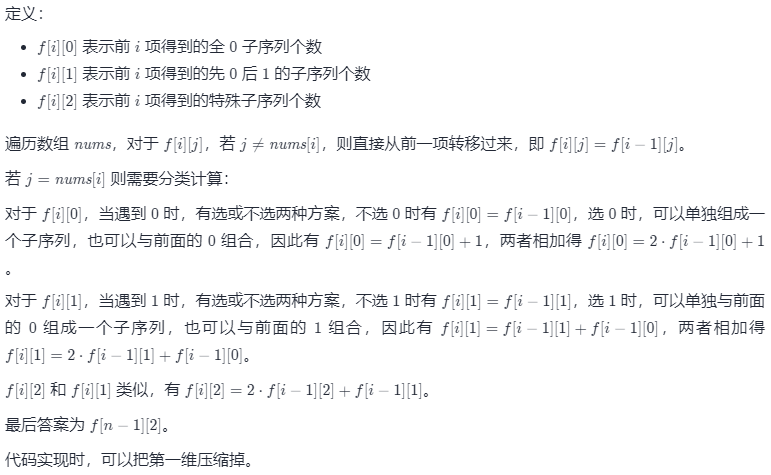
\includegraphics[width=.9\linewidth]{./pic/specialSeq.png}

\begin{minted}[frame=lines,fontsize=\scriptsize,linenos=false]{java}
public int countSpecialSubsequences(int[] arr) { // 去找个降维的参考一下
    int mod = (int)1e9 + 7;
    int n = arr.length;
    long [][] dp = new long [n][3];
    for (int i = 0; i < n; i++) 
        for (int j = 0; j < 3; j++) {
            if (arr[i] != j) dp[i][j] = (i == 0 ? 0 : dp[i-1][j]);
            else 
                if (j == 0)
                    dp[i][j] = (i == 0 ? 0 : dp[i-1][j]) * 2 % mod + 1;
                else
                    dp[i][j] = ((i == 0 ? 0 : dp[i-1][j]) * 2 % mod + (i == 0 ? 0 : dp[i-1][j-1])) % mod;
        }
    return (int)dp[n-1][2];
}
\end{minted}

\chapter{HashMap}
\label{sec-3}
\section{数有多少个数组数不清楚}
\label{sec-3-1}
\section{336. Palindrome Pairs - Hard}
\label{sec-3-2}
Given a list of unique words, return all the pairs of the distinct indices (i, j) in the given list, so that the concatenation of the two words words[i] + words[j] is a palindrome.
\subsection{解题思路与分析}
\label{sec-3-2-1}
\begin{itemize}
\item 利用字典wmap保存单词 -> 下标的键值对
\item 遍历单词列表words,记当前单词为word,下标为idx:
\end{itemize}
\begin{minted}[frame=lines,fontsize=\scriptsize,linenos=false]{java}
1). 若当前单词word本身为回文,且words中存在空串,则将空串下标bidx与idx加入答案
2). 若当前单词的逆序串在words中,则将逆序串下标ridx与idx加入答案
3). 将当前单词word拆分为左右两半left,right。
     3.1) 若left为回文,并且right的逆序串在words中,则将right的逆序串下标rridx与idx加入答案
     3.2) 若right为回文,并且left的逆序串在words中,则将left的逆序串下标idx与rlidx加入答案
\end{minted}

情况分析清楚以后,针对每个情况逐个判断, 然后提前建好hashmap以后判断就好。

细节部分是不要忘记空字符串的情况, 然后针对整个字符串反过来的情况,不要有重复。
\begin{minted}[frame=lines,fontsize=\scriptsize,linenos=false]{java}
private boolean isPalindrome(String s, int i, int j) {
    while (i < j) 
        if (s.charAt(i++) != s.charAt(j--)) return false;
    return true;
}
public List<List<Integer>> palindromePairs(String[] words) {
    Map<String, Integer> map = new HashMap<>();
    List<List<Integer>> ans = new ArrayList<>();
    for (int i = 0; i < words.length; i++) 
        map.put(words[i], i);
    for (int i = 0; i < words.length; i++) {
        if (words[i].equals("")) {
            for (int j = 0; j < words.length; j++) {
                String w = words[j];
                if (isPalindrome(w, 0, w.length()-1) && j != i) {
                    ans.add(List.of(i, j));
                    ans.add(List.of(j, i));
                }
            }
            continue;
        }
        StringBuilder sb = new StringBuilder(words[i]);
        sb.reverse();
        String bw = sb.toString();
        if (map.containsKey(bw)) {
            int res = map.get(bw);
            if (res != i) ans.add(List.of(i, res));
        }
        for (int j = 1; j < bw.length(); j++) {
            if (isPalindrome(bw, 0, j-1)) {
                String s = bw.substring(j);
                if (map.containsKey(s))
                    ans.add(List.of(i, map.get(s)));
            }
            if (isPalindrome(bw, j, bw.length()-1)) {
                String s = bw.substring(0, j);
                if (map.containsKey(s))
                    ans.add(List.of(map.get(s), i));
            }
        }
    }
    return ans;
}
\end{minted}

\section{1392. Longest Happy Prefix - Hard}
\label{sec-3-3}
A string is called a happy prefix if is a non-empty prefix which is also a suffix (excluding itself).

Given a string s, return the longest happy prefix of s. Return an empty string "" if no such prefix exists.
\begin{minted}[frame=lines,fontsize=\scriptsize,linenos=false]{java}
// 频繁的字符串操作(substring和equals操作)会大幅消耗执行时间,也会导致TLE时间超时。
// 因此我们可以使用字符串的hash值方式来比较前后缀是否相同。这里我们需要普及一个知识点,任意一个字符串的Hash值的计算公式为:
// int hash=s[0]∗31^(n−1)+s[1]∗31^(n−2) +...+s[n−2]∗31^1+s[n−1]∗31^0
//     对于前缀hash,每次长度加一后hash的变化应该是:
//     hash = hash*31 + 新添头字符ch
//     对于后缀hash,每次长度加一后hash的变化应该是:
//     hash = hash + 新添尾字符*31^t   (t为后缀长度减1)
//     这样我们每次只需要比较前缀hash与后缀hash是否相同即可。
public String longestPrefix(String s) {
    int n = s.length(), hashPre = 0, hashSuf = 0;
    int left = 0, right = n-1, pow = 1, maxLen = 0;
    String res = "";
    while (left < n-1) {
        hashPre = hashPre * 31 + s.charAt(left);
        hashSuf = hashSuf + s.charAt(right)*pow;
        if (hashPre == hashSuf) maxLen = left + 1;
        left ++;
        right --;
        pow *= 31;
    }
    return maxLen == 0 ? "" : s.substring(0, maxLen);
}
\end{minted}
\subsection{KMP 算法}
\label{sec-3-3-1}
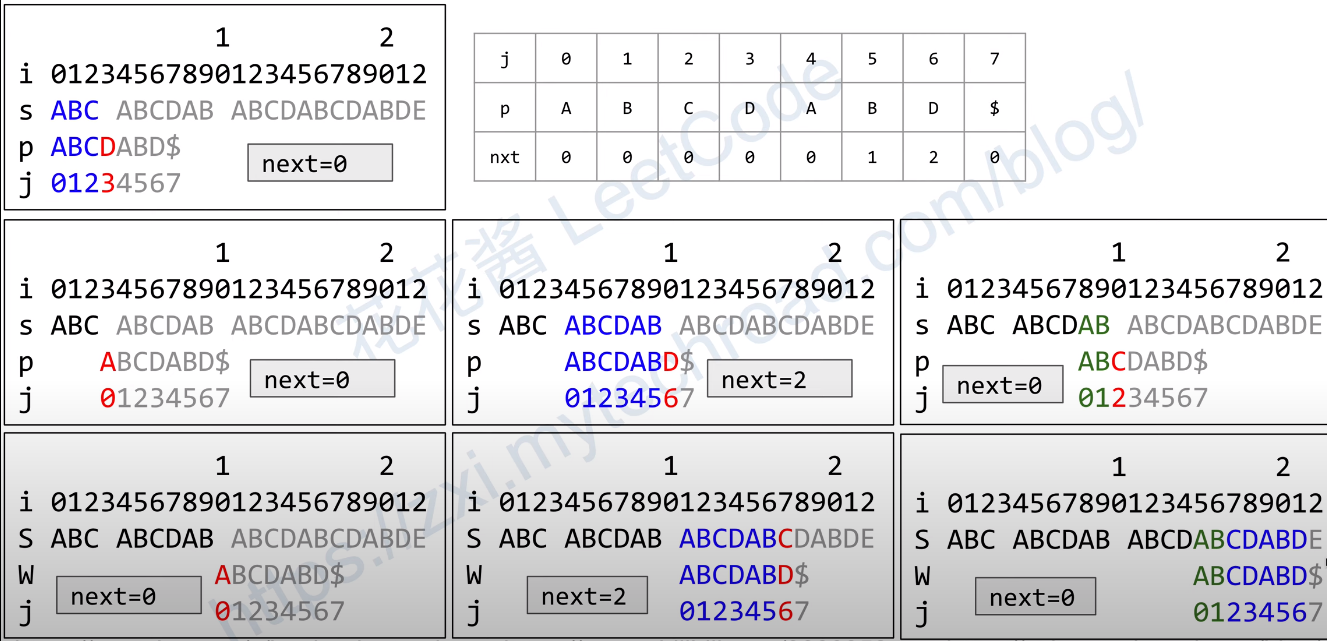
\includegraphics[width=.9\linewidth]{./pic/kmp.png}

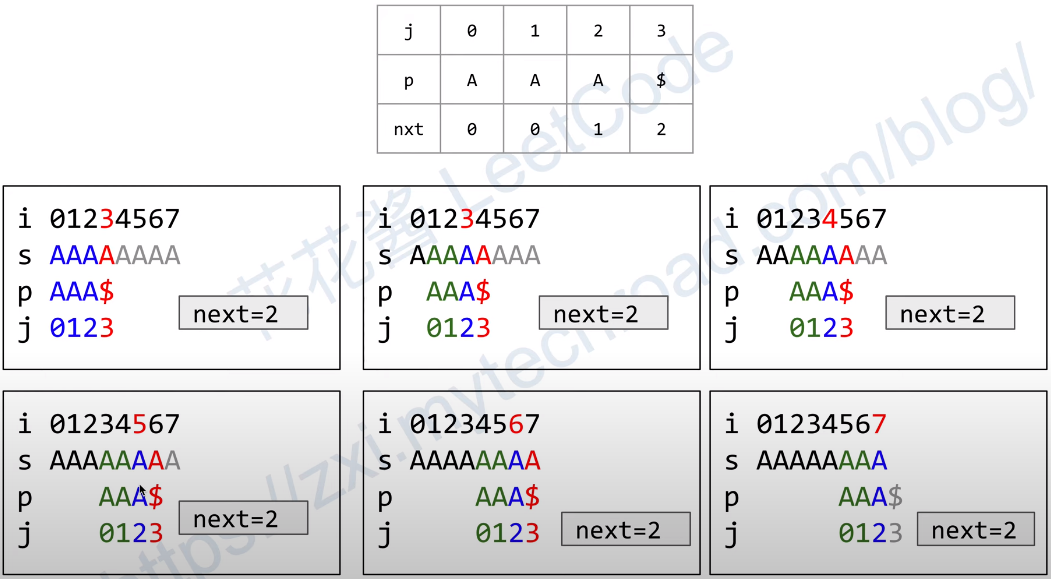
\includegraphics[width=.9\linewidth]{./pic/kmp2.png}

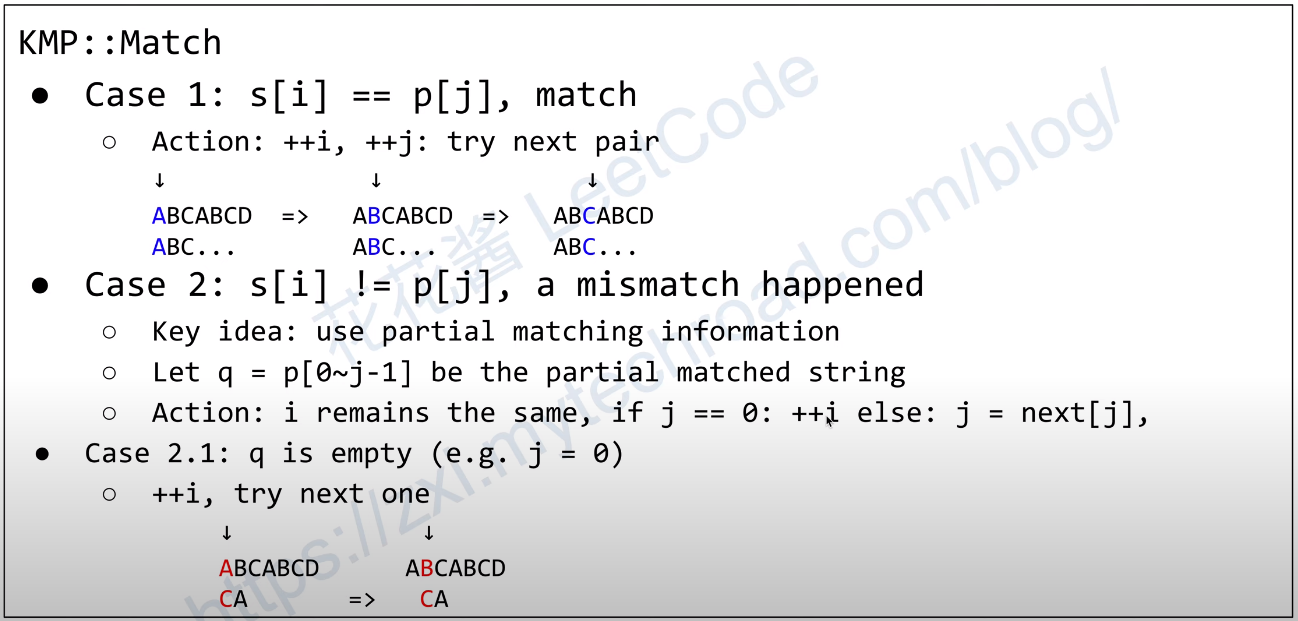
\includegraphics[width=.9\linewidth]{./pic/kmp3.png}

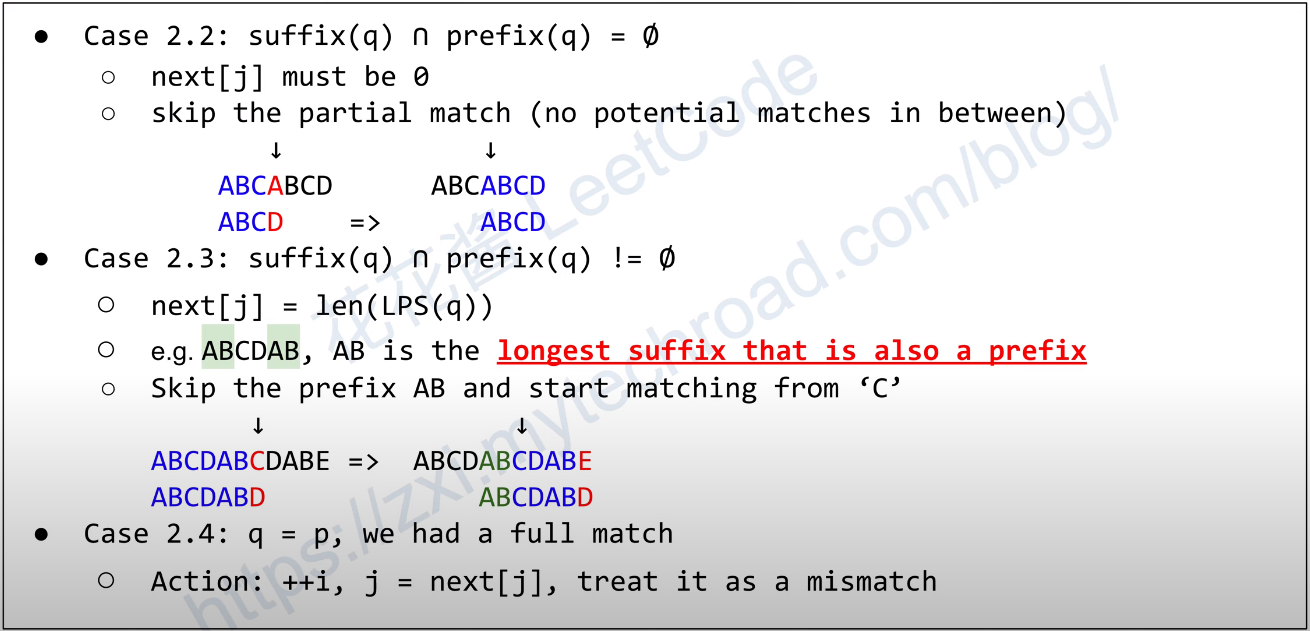
\includegraphics[width=.9\linewidth]{./pic/kmp4.png}

\begin{minted}[frame=lines,fontsize=\scriptsize,linenos=false]{java}
// straight forward KMP algorithm - 8ms - beats 94% time - O(N) time and O(N) space
public String longestPrefix(String s) {
    int i, x, N = s.length();
    int [] LPS = new int[N];
    LPS[0] = 0;
    for (i = 1; i < N; i++){
        x = LPS[i - 1];
        while (s.charAt(i) != s.charAt(x)){
            if (x == 0){
                x = -1;
                break;
            }
            x = LPS[x - 1];
        }
        LPS[i] = x + 1;
    }
    return s.substring(0, LPS[N - 1]);
}
\end{minted}
\begin{minted}[frame=lines,fontsize=\scriptsize,linenos=false]{cpp}
string longestPrefix(string s) {
    vector<int> lps(s.size(), 0);
    size_t i = 0, j = 1;
    while (j < s.size()) {
        if (s[i] == s[j]) lps[j++] = (i++) + 1;  // situ.1
        else if (i != 0) i = lps[i - 1];         // situ.2
        else lps[j++] = 0;                       // situ.3
    }
    return s.substr(0, lps.back());
}
\end{minted}
\section{1172. Dinner Plate Stacks - Hard}
\label{sec-3-4}
You have an infinite number of stacks arranged in a row and numbered (left to right) from 0, each of the stacks has the same maximum capacity.

Implement the DinnerPlates class:

DinnerPlates(int capacity) Initializes the object with the maximum capacity of the stacks capacity.
void push(int val) Pushes the given integer val into the leftmost stack with a size less than capacity.
int pop() Returns the value at the top of the rightmost non-empty stack and removes it from that stack, and returns -1 if all the stacks are empty.
int popAtStack(int index) Returns the value at the top of the stack with the given index index and removes it from that stack or returns -1 if the stack with that given index is empty.
\begin{minted}[frame=lines,fontsize=\scriptsize,linenos=false]{java}
    Stack<Stack<Integer>> stacks = new Stack<>();
    TreeSet<Integer> set = new TreeSet<>(); // set: 
    int capacity;
    public DinnerPlates(int capacity) {
        this.capacity = capacity;
        stacks = new Stack<>();
    }
    public void push(int val) {
        if (set.size() != 0) {
            int idx = set.iterator().next();
            stacks.get(idx).push(val);
            if (stacks.get(idx).size() == capacity)
                set.remove(idx);
        } else {
            if (stacks.isEmpty() || stacks.peek().size() == capacity) {
                stacks.add(new Stack<>()); // 更高效一点儿?
                // stacks.push(new Stack<>());
                stacks.peek().add(val);
            } else stacks.peek().add(val);
        }
    }
    public int pop() {
        if (!stacks.isEmpty()) {
            int k = stacks.peek().pop();
            while (!stacks.isEmpty() && stacks.peek().isEmpty()) {
                set.remove(stacks.size()-1);
                stacks.pop();
            }
            return k;
        }
        return -1;
    }
    public int popAtStack(int index) {
        if (index >= stacks.size() || stacks.get(index).size() == 0) 
            return -1;
        if (index == stacks.size()-1)
            return this.pop();
        set.add(index);
        return stacks.get(index).pop();
    }
\end{minted}
\begin{itemize}
\item 用了双端队列的一个方法
\end{itemize}
\begin{minted}[frame=lines,fontsize=\scriptsize,linenos=false]{java}
    List<Deque<Integer>> stackList = new ArrayList<>();
    TreeSet<Integer> pushIdxSet = new TreeSet<>();
    TreeSet<Integer> popIdxSet = new TreeSet<>();
    int capacity;
    public DinnerPlates(int capacity) {
        stackList = new ArrayList<>();
        pushIdxSet = new TreeSet<>();
        popIdxSet = new TreeSet<>();
        this.capacity = capacity;
        stackList.add(new ArrayDeque<>());
        pushIdxSet.add(0);
    }
    public void push(int val) {
        int idx = pushIdxSet.first();
        if (stackList.get(idx).isEmpty()) 
            popIdxSet.add(idx);
        stackList.get(idx).offerLast(val);
        if (stackList.get(idx).size() == capacity) {
            if (idx == stackList.size() - 1) {
                stackList.add(new ArrayDeque<>());
                pushIdxSet.add(idx + 1);
            }
            pushIdxSet.remove(idx);
        }
    }
    public int pop() {
        if (popIdxSet.isEmpty()) return -1;
        int idx = popIdxSet.last();
        if (stackList.get(idx).size() == capacity)
            pushIdxSet.add(idx);
        int res = stackList.get(idx).pollLast();
        if (stackList.get(idx).isEmpty())
            popIdxSet.remove(idx);
        return res;
    }
    public int popAtStack(int index) {
        if (index >= stackList.size()) return -1;
        if (stackList.get(index).isEmpty()) return -1;
        if (stackList.get(index).size() == capacity)
            pushIdxSet.add(index);
        int res = stackList.get(index).pollLast();
        if (stackList.get(index).isEmpty()) 
            popIdxSet.remove(index);
        return res;
    }
\end{minted}


\chapter{Tree}
\label{sec-4}
\section{979. Distribute Coins in Binary Tree}
\label{sec-4-1}
You are given the root of a binary tree with n nodes where each node in the tree has node.val coins. There are n coins in total throughout the whole tree.

In one move, we may choose two adjacent nodes and move one coin from one node to another. A move may be from parent to child, or from child to parent.

Return the minimum number of moves required to make every node have exactly one coin.
\begin{minted}[frame=lines,fontsize=\scriptsize,linenos=false]{java}
private int dfs(TreeNode r) { // 统计把自身,左右子树都平衡,需要移动的coins个数
    if (r == null) return 0;
    int left = dfs(r.left);      // 左、右子树缺多少
    int right = dfs(r.right);
    res += Math.abs(left) + Math.abs(right); // 左,右子树和自身都平衡需要的移动数
    return left + right + r.val-1;
}
int res;
public int distributeCoins(TreeNode root) {
    res = 0;
    return res;
}
\end{minted}

\section{687. Longest Univalue Path}
\label{sec-4-2}
Given the root of a binary tree, return the length of the longest path, where each node in the path has the same value. This path may or may not pass through the root.

The length of the path between two nodes is represented by the number of edges between them.
\begin{itemize}
\item 此题与求二叉树的最长路径边长相似,只是此题要求是节点值相同的路径,也就是说在找最长路径的时候,还需要判断节点值,要是不相同,就重置为0,在此期间,我们使用一个全局变量来存储最长节点值相同路径的边长。
\end{itemize}
\begin{minted}[frame=lines,fontsize=\scriptsize,linenos=false]{java}
private int topDownTraverse(TreeNode r) { 
    if (r == null) return 0;
    int left = topDownTraverse(r.left);
    int right = topDownTraverse(r.right);
    if (r.left == null || r.left.val != r.val) left = 0;
    if (r.right == null || r.right.val != r.val) right = 0;
    max = Math.max(max, left + right);
    return Math.max(left, right) + 1;
}
int max = 0;
public int longestUnivaluePath(TreeNode root) {
    if (root == null) return 0;
    topDownTraverse(root);
    return max;
}
\end{minted}

\section{652. Find Duplicate Subtrees}
\label{sec-4-3}
Given the root of a binary tree, return all duplicate subtrees.

For each kind of duplicate subtrees, you only need to return the root node of any one of them.

Two trees are duplicate if they have the same structure with the same node values.
\begin{minted}[frame=lines,fontsize=\scriptsize,linenos=false]{java}
private String duplicate(TreeNode node) {
    if(node == null) return "X";
    String l = duplicate(node.left);
    String r = duplicate(node.right);
    String s = Integer.toString(node.val) + "-" + l + "-" + r;
    map.put(s, map.getOrDefault(s, 0)+1);
    if (map.get(s) == 2)
        list.add(node);
    return s;
}
HashMap<String,Integer> map = new HashMap<>();
ArrayList list = new ArrayList<>();
public List findDuplicateSubtrees(TreeNode root) {
    duplicate(root);
    return list;
}
\end{minted}
\begin{itemize}
\item 看一下构造的图的效果图
\end{itemize}
\begin{minted}[frame=lines,fontsize=\scriptsize,linenos=false]{java}
      1 -> root
    2, 3,  ->
4, #| 2, 4,  ->
#.#| 4, #| #.#|  ->
#.#|  ->

map.size(): 4
3-2-4-X-X-X-4-X-X, 1
1-2-4-X-X-X-3-2-4-X-X-X-4-X-X, 1
2-4-X-X-X, 2
4-X-X, 3

res.size(): 2
TREE Level order traversal:
      4 -> root
    #.#|  ->

TREE Level order traversal:
      2 -> root
    4, #|  ->
#.#|  ->
\end{minted}
\begin{itemize}
\item 一种dfs的写法
\end{itemize}
\begin{minted}[frame=lines,fontsize=\scriptsize,linenos=false]{java}
HashSet<String> set, added;
List<TreeNode> list;
public List<TreeNode> findDuplicateSubtrees(TreeNode root) {
    set = new HashSet();
    added = new HashSet();
    list = new ArrayList();
    StringBuilder ret = dfs(root);
    return list;
}
private StringBuilder dfs(TreeNode root){
    if (root == null) return null;
    StringBuilder sbL = dfs(root.left), sbR = dfs(root.right);
    if (sbL == null && sbR == null){
        sbL = new StringBuilder();
        sbL.append(root.val);
    } else if (sbL != null){
        sbL.append(" " + root.val);
        if (sbR != null){
            sbL.append(' ');
            sbL.append(sbR);
        } else sbL.append(" n");
    } else if (sbL == null){
        if (sbR != null){
            sbR.insert(0, " n " + root.val);
            sbL = sbR;
        }
    }
    String temp = sbL.toString();
    if (set.contains(temp) && !added.contains(temp)){
        list.add(root);
        added.add(temp);

    }
    set.add(temp);
    return sbL;
}
\end{minted}
\begin{itemize}
\item 这个跑起来很高效,可惜我看不懂。。。。。以后再慢慢消化吧
\item \url{https://leetcode.com/problems/find-duplicate-subtrees/discuss/1418487/Java-beats-99.5-in-time}
\end{itemize}
\begin{minted}[frame=lines,fontsize=\scriptsize,linenos=false]{java}
Map<Integer, Integer> count;           // frequency of each subtree represented in string
Map<List<Integer>, Integer> numberMap; // ** not hashset since it cannot reserve element order
List<TreeNode> ans;
int globalNumber = 1;
public List<TreeNode> findDuplicateSubtrees(TreeNode root) {
    count = new HashMap();
    numberMap = new HashMap();
    ans = new ArrayList();
    collect(root);
    return ans;
}
public int collect(TreeNode node) {
    if (node == null) return 0;
    int leftNumber = collect(node.left);
    int rightNumber = collect(node.right);
    List<Integer> numberExp = new ArrayList<>(); // construct expression
    numberExp.add(node.val);
    numberExp.add(leftNumber);
    numberExp.add(rightNumber);
    if (!numberMap.containsKey(numberExp)) { // update numberMap
        numberMap.put(numberExp, globalNumber);
        globalNumber++;
    }
    // check number frequency. if == 2, meaning duplication then add to result
    int rootNumber = numberMap.get(numberExp).intValue();
    count.put(rootNumber, count.getOrDefault(rootNumber, 0)+1);
    if (count.get(rootNumber) == 2) // not >=2, otherwise ans will have duplicated nodes
        ans.add(node);
    return rootNumber;
}
\end{minted}
\begin{minted}[frame=lines,fontsize=\scriptsize,linenos=false]{java}
count.size(): 4
1, 3
2, 2
3, 1
4, 1
numberMap.size(): 4
2, 1, 0,
2
3, 2, 1,
3
1, 2, 3,
4
4, 0, 0,
1
\end{minted}

\chapter{binary Search}
\label{sec-5}
\section{LeetCode Binary Search Summary 二分搜索法小结}
\label{sec-5-1}
\begin{itemize}
\item \url{https://segmentfault.com/a/1190000016825704}
\item \url{https://www.cnblogs.com/grandyang/p/6854825.html}
\end{itemize}
\subsection{标准二分查找}
\label{sec-5-1-1}
\begin{minted}[frame=lines,fontsize=\scriptsize,linenos=false]{java}
public int search(int[] nums, int target) {
    int left = 0;
    int right = nums.length - 1;
    while (left <= right) {
        int mid = left + ((right - left) >> 1);
        if (nums[mid] == target) return mid;
        else if (nums[mid] > target) 
            right = mid - 1;
        else 
            left = mid + 1;
    }
    return -1;
}
\end{minted}

循环终止的条件包括:

\begin{itemize}
\item 找到了目标值
\item left > right (这种情况发生于当left, mid, right指向同一个数时,这个数还不是目标值,则整个查找结束。)
\end{itemize}

left + ((right -left) >> 1) 对于目标区域长度为奇数而言,是处于正中间的,对于长度为偶数而言,是中间偏左的。因此左右边界相遇时,只会是以下两种情况:

\begin{itemize}
\item left/mid , right (left, mid 指向同一个数,right指向它的下一个数)
\item left/mid/right (left, mid, right 指向同一个数)
\end{itemize}

即因为mid对于长度为偶数的区间总是偏左的,所以当区间长度小于等于2时,mid 总是和 left在同一侧。
\subsection{二分查找左边界}
\label{sec-5-1-2}

利用二分法寻找左边界是二分查找的一个变体,应用它的题目常常有以下几种特性之一:

\begin{itemize}
\item 数组有序,但包含重复元素
\item 数组部分有序,且不包含重复元素
\item 数组部分有序,且包含重复元素
\end{itemize}
\begin{enumerate}
\item 左边界查找类型1
\label{sec-5-1-2-1}

类型1包括了上面说的第一种,第二种情况。

既然要寻找左边界,搜索范围就需要从右边开始,不断往左边收缩,也就是说即使我们找到了nums[mid] == target, 这个mid的位置也不一定就是最左侧的那个边界,我们还是要向左侧查找,所以我们在nums[mid]偏大或者nums[mid]就等于目标值的时候,继续收缩右边界,算法模板如下:
\begin{minted}[frame=lines,fontsize=\scriptsize,linenos=false]{java}
public int search(int[] nums, int target) {
    int left = 0;
    int right = nums.length - 1;
    while (left < right) {
        int mid = left + (right - left) / 2;
        if (nums[mid] < target) 
            left = mid + 1;
        else 
            right = mid;
    }
    return nums[left] == target ? left : -1;
}
\end{minted}

返回值: nums[left] == target ? left : -1

与标准的二分查找不同:

首先,这里的右边界的更新是right = mid,因为我们需要在找到目标值后,继续向左寻找左边界。

其次,这里的循环条件是left < right。

因为在最后left与right相邻的时候,mid和left处于相同的位置(前面说过,mid偏左),则下一步,无论怎样,left, mid, right都将指向同一个位置,如果此时循环的条件是left <= right,则我们需要再进入一遍循环,此时,如果nums[mid] < target还好说,循环正常终止;否则,我们会令right = mid,这样并没有改变left,mid,right的位置,将进入死循环。

事实上,我们只需要遍历到left和right相邻的情况就行了,因为这一轮循环后,无论怎样,left,mid,right都会指向同一个位置,而如果这个位置的值等于目标值,则它就一定是最左侧的目标值;如果不等于目标值,则说明没有找到目标值,这也就是为什么返回值是nums[left] == target ? left : -1。

\begin{minted}[frame=lines,fontsize=\scriptsize,linenos=false]{java}
public int searchInsert(int[] nums, int target) {
    int len = nums.length;
    if (nums[len - 1] < target) return len;
    int left = 0;
    int right = len - 1;
    while (left <= right) {
        int mid = (left + right) / 2;
        // 等于的情况最简单,我们应该放在第 1 个分支进行判断
        if (nums[mid] == target) {
            return mid;
        } else if (nums[mid] < target) {
            // 题目要我们返回大于或者等于目标值的第 1 个数的索引
            // 此时 mid 一定不是所求的左边界,
            // 此时左边界更新为 mid + 1
            left = mid + 1;
        } else {
            // 既然不会等于,此时 nums[mid] > target
            // mid 也一定不是所求的右边界
            // 此时右边界更新为 mid - 1
            right = mid - 1;
        }
    }
    // 注意:一定得返回左边界 left,
    // 理由是对于 [1,3,5,6],target = 2,返回大于等于 target 的第 1 个数的索引,此时应该返回 1
    // 在上面的 while (left <= right) 退出循环以后,right < left,right = 0 ,left = 1
    // 根据题意应该返回 left,
    // 如果题目要求你返回小于等于 target 的所有数里最大的那个索引值,应该返回 right
    return left;
}
\end{minted}
\item 左边界查找类型2
\label{sec-5-1-2-2}

左边界查找的第二种类型用于数组部分有序且包含重复元素的情况,这种条件下在我们向左收缩的时候,不能简单的令 right = mid,因为有重复元素的存在,这会导致我们有可能遗漏掉一部分区域,此时向左收缩只能采用比较保守的方式,代码模板如下:
\begin{minted}[frame=lines,fontsize=\scriptsize,linenos=false]{java}
public int search(int[] nums, int target) {
    int left = 0;
    int right = nums.length - 1;
    while (left < right) {
        int mid = left + (right - left) / 2;
        if (nums[mid] < target) 
            left = mid + 1;
        else if (nums[mid] > target) 
            right = mid;
        else 
            right--;
    }
    return nums[left] == target ? left : -1;
}
\end{minted}

它与类型1的唯一区别就在于对右侧值的收缩更加保守。这种收缩方式可以有效地防止我们一下子跳过了目标边界从而导致了搜索区域的遗漏。
\end{enumerate}

\subsection{二分查找右边界}
\label{sec-5-1-3}
\begin{minted}[frame=lines,fontsize=\scriptsize,linenos=false]{java}
public int search(int[] nums, int target) {
    int left = 0;
    int right = nums.length - 1;
    while (left < right) {
        int mid = left + ((right - left) >> 1) + 1;
        if (nums[mid] > target) 
            right = mid - 1;
        else 
            left = mid;
    }
    return nums[right] == target ? right : -1;
}
\end{minted}
\begin{itemize}
\item 循环条件: left < right
\item 中间位置计算: mid = left + ((right -left) >> 1) + 1
\item 左边界更新:left = mid
\item 右边界更新: right = mid - 1
\item 返回值: nums[right] == target ? right : -1
\end{itemize}

这里大部分和寻找左边界是对称着来写的,唯独有一点需要尤其注意——中间位置的计算变了,我们在末尾多加了1。这样,无论对于奇数还是偶数,这个中间的位置都是偏右的。

对于这个操作的理解,从对称的角度看,寻找左边界的时候,中间位置是偏左的,那寻找右边界的时候,中间位置就应该偏右呗,但是这显然不是根本原因。根本原因是,在最后left和right相邻时,如果mid偏左,则left, mid指向同一个位置,right指向它们的下一个位置,在nums[left]已经等于目标值的情况下,这三个位置的值都不会更新,从而进入了死循环。所以我们应该让mid偏右,这样left就能向右移动。这也就是为什么我们之前一直强调查找条件,判断条件和左右边界的更新方式三者之间需要配合使用。

右边界的查找一般来说不会单独使用,如有需要,一般是需要同时查找左右边界。

\subsection{二分查找左右边界}
\label{sec-5-1-4}
前面我们介绍了左边界和右边界的查找,那么查找左右边界就容易很多了——只要分别查找左边界和右边界就行了。
\subsection{二分查找极值}
\label{sec-5-1-5}
二分查找还有一种有趣的变体是二分查找极值点,之前我们使用nums[mid]去比较的时候,常常是和给定的目标值target比,或者和左右边界比较,在二分查找极值点的应用中,我们是和相邻元素去比,以完成某种单调性的检测。关于这一点,我们直接来看一个例子就明白了。

Find Peak Element

A peak element is an element that is greater than its neighbors.

Given an input array nums, where nums[i] ≠ nums[i+1], find a peak element and return its index.

The array may contain multiple peaks, in that case return the index to any one of the peaks is fine.

You may imagine that nums[-1] = nums[n] = -∞.

这一题的有趣之处在于他要求求一个局部极大值点,并且整个数组不包含重复元素。所以整个数组甚至可以是无序的——你可能很难想象我们可以在一个无序的数组中直接使用二分查找,但是没错!我们确实可以这么干!谁要人家只要一个局部极大值即可呢。
\begin{minted}[frame=lines,fontsize=\scriptsize,linenos=false]{java}
public int findPeakElement(int[] nums) {
    int left = 0;
    int right = nums.length - 1;
    while (left < right) {
        int mid = left + ((right - left) >> 1);
        if (nums[mid] < nums[mid + 1]) 
            left = mid + 1;
        else 
            right = mid;
    }
    return left;
}
\end{minted}
\begin{minted}[frame=lines,fontsize=\scriptsize,linenos=false]{java}
public int binarySearch2(int[] nums, int target) {
    // left和right都在数组下标范围内
    // [left, right]
    int left = 0;
    int right = nums.length - 1;
    // while循环跳出的条件是left > right
    // 所以如果没找到target的话,也不需要特判了
    while (left <= right) {
        int mid = left + (right - left) / 2;
        if (nums[mid] == target) return mid;
        else if (nums[mid] < target) 
            left = mid + 1;
        else
            right = mid - 1;
    }
    // 如果没找到就只能返回-1
    return -1;
}
// 模板二,适合判断当前 index 和 index + 1 之间的关系。
// right 指针一开始的定义是在数组下标范围外的,[left, right),所以在需要移动 right 指针的时候不能写成 right = mid。这样会遗漏掉一些下标的判断。
public int binarySearch3(int[] nums, int target) {
    // right不在下标范围内
    // [left, right)
    int left = 0;
    int right = nums.length;
    // while循环跳出的条件是left == right
    // 这个模板比较适合判断当前index和index + 1之间的关系
    // left < right, example, left = 0, right = 1
    while (left < right) {
        int mid = left + (right - left) / 2;
        if (nums[mid] == target) return mid;
        else if (nums[mid] < target) 
            left = mid + 1;
        else
            // 因为搜索范围是左闭右开所以这里不能-1
            right = mid;
    }
    // 最后的特判
    if (left != nums.length && nums[left] == target) 
        return left;
    return -1;
}
// while条件不满足的时候,left + 1 == right,两下标应该指向某个下标 i 和 i + 1。这样如果有什么特殊的值需要判断,应该不是 left 就是 right 了。
public int binarySearch1(int[] nums, int target) {
    // left和right都在数组下标范围内
    // [left, right]
    int left = 0;
    int right = nums.length - 1;
    // 举例,start - 0, end = 3
    // 中间隔了起码有start + 1和start + 2两个下标
    // 这样跳出while循环的时候,start + 1 == end
    // 才有了最后的两个判断
    while (left + 1 < right) {
        int mid = left + (right - left) / 2;
        if (nums[mid] == target) return mid;
        else if (nums[mid] < target) 
            left = mid;
        else 
            right = mid;
    }
    // 特判
    if (nums[left] == target) return left;
    if (nums[right] == target) return right;
    // 如果没找到就只能返回-1
    return -1;
}
\end{minted}

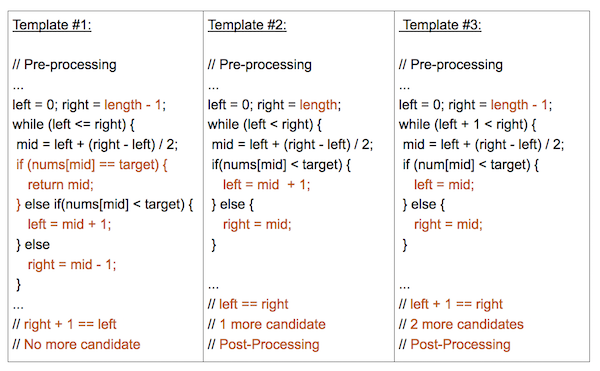
\includegraphics[width=.9\linewidth]{./pic/binarySearch.png} 

\subsection{第一类: 需查找和目标值完全相等的数}
\label{sec-5-1-6}

这是最简单的一类,也是我们最开始学二分查找法需要解决的问题,比如我们有数组 [2, 4, 5, 6, 9],target = 6,那么我们可以写出二分查找法的代码如下:
\begin{minted}[frame=lines,fontsize=\scriptsize,linenos=false]{c++}
int find(vector<int>& nums, int target) {
    int left = 0, right = nums.size();
    while (left < right) {
        int mid = left + (right - left) / 2;
        if (nums[mid] == target) return mid;
        else if (nums[mid] < target) left = mid + 1;
        else right = mid;
    }
    return -1;
}
\end{minted}

会返回3,也就是 target 的在数组中的位置。注意二分查找法的写法并不唯一,主要可以变动地方有四处:

第一处是 right 的初始化,可以写成 nums.size() 或者 nums.size() - 1。

第二处是 left 和 right 的关系,可以写成 left < right 或者 left <= right。

第三处是更新 right 的赋值,可以写成 right = mid 或者 right = mid - 1。

第四处是最后返回值,可以返回 left,right,或 right - 1。

\begin{itemize}
\item 但是这些不同的写法并不能随机的组合,像博主的那种写法,
\begin{itemize}
\item 若 right 初始化为了 nums.size(),那么就必须用 left < right,而最后的 right 的赋值必须用 right = mid。
\item 但是如果我们 right 初始化为 nums.size() - 1,那么就必须用 left <= right,并且right的赋值要写成 right = mid - 1,不然就会出错。
\end{itemize}
\end{itemize}

所以博主的建议是选择一套自己喜欢的写法,并且记住,实在不行就带简单的例子来一步一步执行,确定正确的写法也行。

第一类应用实例:

Intersection of Two Arrays

\subsection{第二类: 查找第一个不小于目标值的数,可变形为查找最后一个小于目标值的数}
\label{sec-5-1-7}

这是比较常见的一类,因为我们要查找的目标值不一定会在数组中出现,也有可能是跟目标值相等的数在数组中并不唯一,而是有多个,那么这种情况下 nums[mid] == target 这条判断语句就没有必要存在。比如在数组 [2, 4, 5, 6, 9] 中查找数字3,就会返回数字4的位置;在数组 [0, 1, 1, 1, 1] 中查找数字1,就会返回第一个数字1的位置。我们可以使用如下代码:
\begin{minted}[frame=lines,fontsize=\scriptsize,linenos=false]{c++}
int find(vector<int>& nums, int target) {
    int left = 0, right = nums.size();
    while (left < right) {
        int mid = left + (right - left) / 2;
        if (nums[mid] < target) left = mid + 1;
        else right = mid;
    }
    return right;
}
\end{minted}

最后我们需要返回的位置就是 right 指针指向的地方。在 C++ 的 STL 中有专门的查找第一个不小于目标值的数的函数 lower$_{\text{bound,在博主的解法中也会时不时的用到这个函数。但是如果面试的时候人家不让使用内置函数,那么我们只能老老实实写上面这段二分查找的函数。}}$

这一类可以轻松的变形为查找最后一个小于目标值的数,怎么变呢。我们已经找到了第一个不小于目标值的数,那么再往前退一位,返回 right - 1,就是最后一个小于目标值的数。

第二类应用实例:

Heaters, Arranging Coins, Valid Perfect Square,Max Sum of Rectangle No Larger Than K,Russian Doll Envelopes

第二类变形应用:Valid Triangle Number

\subsection{第三类: 查找第一个大于目标值的数,可变形为查找最后一个不大于目标值的数}
\label{sec-5-1-8}

这一类也比较常见,尤其是查找第一个大于目标值的数,在 C++ 的 STL 也有专门的函数 upper$_{\text{bound,这里跟上面的那种情况的写法上很相似,只需要添加一个等号,将之前的}}$ nums[mid] < target 变成 nums[mid] <= target,就这一个小小的变化,其实直接就改变了搜索的方向,使得在数组中有很多跟目标值相同的数字存在的情况下,返回最后一个相同的数字的下一个位置。比如在数组 [2, 4, 5, 6, 9] 中查找数字3,还是返回数字4的位置,这跟上面那查找方式返回的结果相同,因为数字4在此数组中既是第一个不小于目标值3的数,也是第一个大于目标值3的数,所以 make sense;在数组 [0, 1, 1, 1, 1] 中查找数字1,就会返回坐标5,通过对比返回的坐标和数组的长度,我们就知道是否存在这样一个大于目标值的数。参见下面的代码:
\begin{minted}[frame=lines,fontsize=\scriptsize,linenos=false]{c++}
int find(vector<int>& nums, int target) {
    int left = 0, right = nums.size();
    while (left < right) {
        int mid = left + (right - left) / 2;
        if (nums[mid] <= target) left = mid + 1;
        else right = mid;
    }
    return right;
}
\end{minted}

这一类可以轻松的变形为查找最后一个不大于目标值的数,怎么变呢。我们已经找到了第一个大于目标值的数,那么再往前退一位,返回 right - 1,就是最后一个不大于目标值的数。比如在数组 [0, 1, 1, 1, 1] 中查找数字1,就会返回最后一个数字1的位置4,这在有些情况下是需要这么做的。

第三类应用实例:

Kth Smallest Element in a Sorted Matrix

第三类变形应用示例:

Sqrt(x)

\subsection{第四类: 用子函数当作判断关系(通常由 mid 计算得出)}
\label{sec-5-1-9}

这是最令博主头疼的一类,而且通常情况下都很难。因为这里在二分查找法重要的比较大小的地方使用到了子函数,并不是之前三类中简单的数字大小的比较,比如 Split Array Largest Sum 那道题中的解法一,就是根据是否能分割数组来确定下一步搜索的范围。类似的还有 Guess Number Higher or Lower 这道题,是根据给定函数 guess 的返回值情况来确定搜索的范围。对于这类题目,博主也很无奈,遇到了只能自求多福了。

第四类应用实例:

Split Array Largest Sum, Guess Number Higher or Lower,Find K Closest Elements,Find K-th Smallest Pair Distance,Kth Smallest Number in Multiplication Table,Maximum Average Subarray II,Minimize Max Distance to Gas Station,Swim in Rising Water,Koko Eating Bananas,Nth Magical Number

\subsection{第五类: 其他(通常 target 值不固定)}
\label{sec-5-1-10}

有些题目不属于上述的四类,但是还是需要用到二分搜索法,比如这道 Find Peak Element,求的是数组的局部峰值。由于是求的峰值,需要跟相邻的数字比较,那么 target 就不是一个固定的值,而且这道题的一定要注意的是 right 的初始化,一定要是 nums.size() - 1,这是由于算出了 mid 后,nums[mid] 要和 nums[mid+1] 比较,如果 right 初始化为 nums.size() 的话,mid+1 可能会越界,从而不能找到正确的值,同时 while 循环的终止条件必须是 left < right,不能有等号。

类似的还有一道 H-Index II,这道题的 target 也不是一个固定值,而是 len-mid,这就很意思了,跟上面的 nums[mid+1] 有异曲同工之妙,target 值都随着 mid 值的变化而变化,这里的right的初始化,一定要是 nums.size() - 1,而 while 循环的终止条件必须是 left <= right,这里又必须要有等号,是不是很头大 -.-!!!

其实仔细分析的话,可以发现其实这跟第四类还是比较相似,相似点是都很难 -.-!!!,第四类中虽然是用子函数来判断关系,但大部分时候 mid 也会作为一个参数带入子函数进行计算,这样实际上最终算出的值还是受 mid 的影响,但是 right 却可以初始化为数组长度,循环条件也可以不带等号,大家可以对比区别一下~

第五类应用实例:

Find Peak Element

H-Index II

\section{793. Preimage Size of Factorial Zeroes Function}
\label{sec-5-2}
Let f(x) be the number of zeroes at the end of x!. Recall that x! = 1 * 2 * 3 * \ldots{} * x and by convention, 0! = 1.

For example, f(3) = 0 because 3! = 6 has no zeroes at the end, while f(11) = 2 because 11! = 39916800 has two zeroes at the end.
Given an integer k, return the number of non-negative integers x have the property that f(x) = k.

\begin{minted}[frame=lines,fontsize=\scriptsize,linenos=false]{java}
private long numberOfTrailingZeros(long v) {
    long cnt = 0;
    for (; v > 0; v /= 5) 
        cnt += v / 5;
    return cnt;
}
public int preimageSizeFZF(int k) {
    long left = 0, right = 5l * (k + 1);
    while (left < right) {
        long mid = left + (right - left) / 2;
        long cnt = numberOfTrailingZeros(mid);
        if (cnt == k) return 5;
        if (cnt < k) left = mid + 1;
        else right = mid;
    }
    return 0;
}
\end{minted}
\begin{itemize}
\item 下面这种解法是把子函数融到了 while 循环内,使得看起来更加简洁一些,解题思路跟上面的解法一模一样,参见代码如下:
\end{itemize}
\begin{minted}[frame=lines,fontsize=\scriptsize,linenos=false]{java}
public int preimageSizeFZF(int k) {
    long left = 0, right = 5l * (k + 1);
    while (left < right) {
        long mid = left + (right - left) / 2, cnt = 0;
        for (long i = 5; mid / i > 0; i *= 5) 
            cnt += mid / i;
        if (cnt == k) return 5;
        if (cnt < k) left = mid + 1;
        else right = mid;
    }
    return 0;
}
\end{minted}

下面这种解法也挺巧妙的,也是根据观察规律推出来的,我们首先来看x为1到 25 的情况:
\begin{minted}[frame=lines,fontsize=\scriptsize,linenos=false]{java}
x:    1 2 3 4 5 6 7 8 9 10 11 12 13 14 15 16 17 18 19 20 21 22 23 24 25
f(x): 0 0 0 0 1 1 1 1 1 2  2  2  2  2  3  3  3  3  3  4  4  4  4  4  6
g(x): 0 0 0 0 1 0 0 0 0 1  0  0  0  0  1  0  0  0  0  1  0  0  0  0  2
\end{minted}

这里,f(x) 是表示 x! 末尾零的个数,而 g(x) = f(x) - f(x-1),其实还可以通过观察发现,f(x) = sum(g(x)).

再仔细观察上面的数字,发现 g(x) 有正值的时候都是当x是5的倍数的时候,那么来专门看一下x是5的倍数时的情况吧:

\begin{minted}[frame=lines,fontsize=\scriptsize,linenos=false]{java}
x:    5 10 15 20 25 30 35 40 45 50 55 60 65 70 75 80 85 90 95 100 105 110 115 120 125
g(x): 1 1  1  1  2  1  1  1  1  2  1  1  1  1  2  1  1  1  1   2   1   1   1   1   3
\end{minted}

仔细观察上面的红色数字,g(x)=1 时,是5的倍数,g(x)=2 时,都是 25 的倍数,g(x)=3 时,是 125 的倍数,那么就有:
\begin{minted}[frame=lines,fontsize=\scriptsize,linenos=false]{java}
g(x) = 0     if x % 5 != 0,
g(x) >= 1    if x % 5 == 0,
g(x) >= 2   if x % 25 == 0.
\end{minted}

如果继续将上面的数字写下去,就可以发现规律,g(x) 按照 1 1 1 1 x 的规律重复五次,第五次的时候x自增1。再继续观察:

当 x=25 时,g(x)=2,此时 K=5 被跳过了。

当 x=50 时,g(x)=2,此时 K=11 被跳过了。

当 x=75 时,g(x)=2,此时 K=17 被跳过了。

当 x=100 时,g(x)=2,此时 K=23 被跳过了。

当 x=125 时,g(x)=3,此时 K=29,30 被跳过了。

进一步,可以发现如下规律:

5(=1*5), 11(=6*1+5), 17(=6*2+5), 23(=6*3+5), 29(=6*4+5), 30(=6*5), 36(=31+5), 42(=31+6+5), 48(=31+6*2+5)

这些使得x不存在的K,出现都是有规律的,它们减去一个特定的基数 base 后,都是余5,而余 1,2,3,4 的,都是返回5。那么这个基 数base,实际是 1,6,31,156,\ldots{},是由 base = base * 5 + 1,不断构成的,通过这种不断对基数取余的操作,可以最终将K降为小于等于5的数,就可以直接返回结果了,参见代码如下:
\begin{minted}[frame=lines,fontsize=\scriptsize,linenos=false]{java}
public int preimageSizeFZF(int k) {
    if (k < 5) return 5;
    int base = 1;
    while (base * 5 + 1 <= k) 
        base = base * 5 + 1;
    if (k / base == 5) return 0;
    return preimageSizeFZF(k % base);
}
\end{minted}

\section{2040. Kth Smallest Product of Two Sorted Arrays - Hard}
\label{sec-5-3}
Given two sorted 0-indexed integer arrays nums1 and nums2 as well as an integer k, return the kth (1-based) smallest product of nums1[i] * nums2[j] where 0 <= i < nums1.length and 0 <= j < nums2.length.

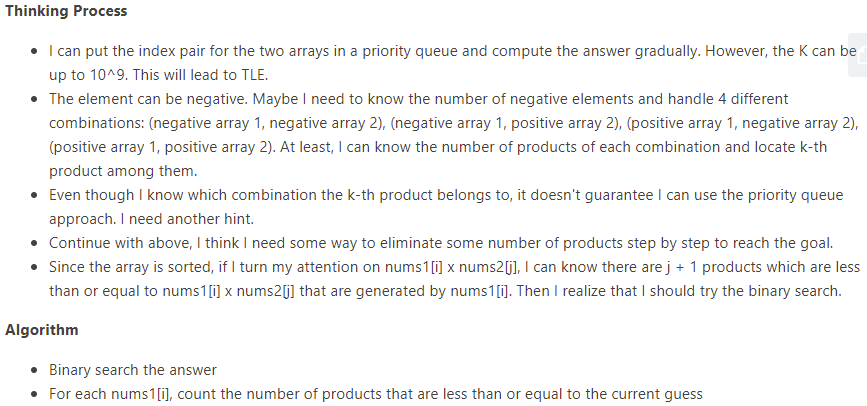
\includegraphics[width=.9\linewidth]{./pic/binarySearch2.png}

\begin{minted}[frame=lines,fontsize=\scriptsize,linenos=false]{java}
private static long INF = (long)1e10;
public long kthSmallestProduct(int[] a, int[] b, long k) { 
    int m = a.length, n = b.length;
    long lo = -INF-1, hi = INF + 1;
    while (lo < hi) {
        long mid = lo + (hi - lo) / 2, cnt = 0;
        for (int  i : a) { // 对于数组a中的每一个数与b中元素的乘积,数<=mid的个数,二分搜索
            if (i >= 0) {
                int l = 0, r = n-1, p = 0;
                while (l <= r) {
                    int c = l + (r - l) / 2;
                    long mul = i * (long)b[c];
                    if (mul <= mid) {
                        p = c + 1;
                        l = c + 1;
                    } else r = c - 1;
                }
                cnt += p;
            } else { // i < 0
                int l = 0, r = n-1, p = 0;
                while (l <= r) {
                    int c = l + (r - l) / 2;
                    long mul = i * (long)b[c];
                    if (mul <= mid) {
                        p = n - c; // i < 0, 数右边<= mid的个数
                        r = c - 1;
                    } else l = c + 1;
                }
                cnt += p;
            }
        }
        if (cnt >= k) hi = mid;
        else lo = mid + 1l;
    }
    return lo;
}
\end{minted}
\begin{itemize}
\item 另一种相当于换汤不换药的写法
\end{itemize}
\begin{minted}[frame=lines,fontsize=\scriptsize,linenos=false]{java}
private static long INF = (long)1e10;
public long kthSmallestProduct(int[] a, int[] b, long k) { 
    long lo = -INF, hi = INF;
    while (lo < hi) {
        long mid = lo + hi + 1 >> 1;
        if (f(a, b, mid) < k) lo = mid;
        else hi = mid - 1;
    }
    return lo;
}
private long f(int [] a, int [] b, long mid) {
    long cnt = 0;
    for (int v : a) {
        int l = 0, r = b.length;
        if (v < 0) {
            while (l < r) {
                int m = l + r >> 1;
                if ((long)v * b[m] >= mid) l = m + 1;
                else r = m;
            }
            cnt += b.length - l;
        } else { // v >= 0
            while (l < r) {
                int m = l + r >> 1;
                if ((long)v * b[m] < mid) l = m + 1;
                else r = m;
            }
            cnt += l;
        }
    }
    return cnt;
}
\end{minted}

\chapter{字符串}
\label{sec-6}
\section{总结}
\label{sec-6-1}
\begin{itemize}
\item KMP算法
\item Rabin-Karp Rolling Hash算法
\item 
\end{itemize}

\section{1910. Remove All Occurrences of a Substring - Medium 可用KMP算法}
\label{sec-6-2}
Given two strings s and part, perform the following operation on s until all occurrences of the substring part are removed:

Find the leftmost occurrence of the substring part and remove it from s.
Return s after removing all occurrences of part.

A substring is a contiguous sequence of characters in a string.
\begin{minted}[frame=lines,fontsize=\scriptsize,linenos=false]{java}
public String removeOccurrences(String s, String part) {
    if (!s.contains(part)) return s;
    int n = s.length();
    int m = part.length();
    while (s.contains(part)) {
        int idx = s.indexOf(part);
        s = s.substring(0, idx) + (idx+m-1 == n-1 ? "" : s.substring(idx+m));
    }
    return s;
}
\end{minted}
\begin{itemize}
\item 有人用了KMP: 字符串匹配可以用KMP算法,由于p pp始终不变,可以先算一下p pp的next数组,然后每次从s ss中找p pp的第一次出现,删去之,再重复进行这个过程
\end{itemize}
\begin{minted}[frame=lines,fontsize=\scriptsize,linenos=false]{java}
private int [] buildNext(String s) { // 找与每个位置字符不同的下一个字母的idx
    int [] next = new int [s.length()];
    for (int i = 0, j = next[0] = -1; i < s.length()-1; ) {
        if (j == -1 || s.charAt(i) == s.charAt(j)) {
            i++;
            j++;
            next[i] = s.charAt(i) != s.charAt(j) ? j : next[j];
        } else j = next[j];
    }
    return next;
}
private int kmp(String s, String p, int [] next) { // 像是夹生饭,半生不熟的
    for (int i = 0, j = 0; i < s.length(); ) {
        if (j == -1 || s.charAt(i) == p.charAt(j)) {
            i++;
            j++;
        } else j = next[j];
        if (j == p.length()) return i-j;
    }
    return -1;
}
public String removeOccurrences(String s, String part) {
    int [] next = buildNext(part);
    int idx = -1;
    while ((idx = kmp(s, part, next)) != -1) 
        s = s.substring(0, idx) + s.substring(idx + part.length());
    return s;
}
\end{minted}

\section{467. Unique Substrings in Wraparound String - Medium Rabin-Karp Rolling Hash算法}
\label{sec-6-3}
We define the string s to be the infinite wraparound string of "abcdefghijklmnopqrstuvwxyz", so s will look like this:

"\ldots{}zabcdefghijklmnopqrstuvwxyzabcdefghijklmnopqrstuvwxyzabcd\ldots{}.".
Given a string p, return the number of unique non-empty substrings of p are present in s.

这道题说有一个无限长的封装字符串,然后又给了我们另一个字符串p,问我们p有多少非空子字符串在封装字符串中。我们通过观察题目中的例子可以发现,由于封装字符串是26个字符按顺序无限循环组成的,那么满足题意的p的子字符串要么是单一的字符,要么是按字母顺序的子字符串。这道题遍历p的所有子字符串会TLE,因为如果p很大的话,子字符串很多,会有大量的满足题意的重复子字符串,必须要用到trick,而所谓技巧就是一般来说你想不到的方法。我们看abcd这个字符串,以d结尾的子字符串有abcd, bcd, cd, d,那么我们可以发现bcd或者cd这些以d结尾的字符串的子字符串都包含在abcd中,那么我们知道以某个字符结束的最大字符串包含其他以该字符结束的字符串的所有子字符串,说起来很拗口,但是理解了我上面举的例子就行。那么题目就可以转换为分别求出以每个字符(a-z)为结束字符的最长连续字符串就行了,我们用一个数组cnt记录下来,最后在求出数组cnt的所有数字之和就是我们要的结果啦,

\begin{minted}[frame=lines,fontsize=\scriptsize,linenos=false]{java}
public int findSubstringInWraproundString(String p) {
    int n = p.length();
    int [] arr = new int [n];
    int [] cnt = new int [26];
    for (int i = 0; i < n; i++) 
        arr[i] = p.charAt(i) - 'a';
    int res = 0, maxLen = 0;
    for (int i = 0; i < n; i++) {
        if (i > 0 && (arr[i-1]+1) % 26 == arr[i]) // 判断前一个位置上的字符比现位字符小1
            ++maxLen;
        else maxLen = 1;
        cnt[arr[i]] = Math.max(cnt[arr[i]], maxLen);
    }
    for (int i = 0; i < 26; i++) 
        res += cnt[i];
    return res;
}
\end{minted}

\section{1044. Longest Duplicate Substring - Hard}
\label{sec-6-4}
Given a string s, consider all duplicated substrings: (contiguous) substrings of s that occur 2 or more times. The occurrences may overlap.

Return any duplicated substring that has the longest possible length. If s does not have a duplicated substring, the answer is "".
\begin{minted}[frame=lines,fontsize=\scriptsize,linenos=false]{java}
public static int base = 26; // 256
public static int mod = (1 << 31) - 1;
public static boolean match(String str1,String str2) {
    assert str1.length() == str2.length();
    for (int i = 0; i < str1.length(); i++) 
        if (str1.charAt(i) != str2.charAt(i))
            return false; 
    return true; 
}
private String search(String s, int v) { // v: substring length
    int n = s.length();
    long hash = 0L, mp = 1l;             // to avoid overflow, long long long
    Map<Long, List<Integer>> map = new HashMap<>();
    for (int j = 0; j < v; j++) {
        hash = ((hash*base) + s.charAt(j)) % mod;
        if (j >= 1)
            mp = mp * base % mod;        // 先乘好准备好,准备着备用 
    }
    map.computeIfAbsent(hash, k->new ArrayList<>()).add(0);
    for (int i = 1; i+v <= n; i++) {
        hash = ((hash - s.charAt(i-1) * mp % mod + mod) % mod * base % mod + s.charAt(i+v-1)) % mod; // mod 
        if (map.containsKey(hash)) 
            for (int idx : map.get(hash)) 
                if (match(s.substring(i, i+v), s.substring(idx, idx+v)))
                    return s.substring(i, i+v);
        map.computeIfAbsent(hash, k->new ArrayList<>()).add(i);
    }
    return null;
}
public String longestDupSubstring(String s) {
    int n = s.length();
    int l = 0, r = n;
    String res = "";
    while (l <= r) {
        int m = l + (r-l) / 2;
        String tmp = search(s, m);
        if (tmp == null) r = m-1;
        else {
            if (tmp.length() > res.length())
                res = tmp;
            l = m+1;
        }
    }
    return res;
}
\end{minted}

\section{1156. Swap For Longest Repeated Character Substring - Medium}
\label{sec-6-5}
You are given a string text. You can swap two of the characters in the text.

Return the length of the longest substring with repeated characters.

给你一个字符串,如何找最长的重复子串,博主会数连续相同的字符,若此时有一个不同字符出现了,只要后面还有相同的字符,就会继续数下去,因为有一次交换的机会,什么时候停止呢,当再次出现不同字符的时候就停止,或者是当前统计个数等于该字符出现的总个数时也停止,因为得到的结果不可能超过某个字符出现的总个数。所以可以先统计每个字符的出现次数,然后开始遍历字符,对于每个遍历到的字符,都开始数之后跟其相等的字符,新建变量j,cnt,和 diff,当j小于n,且当前字符和比较字符相同,或者 diff 等于0,且 cnt 小于比较字符出现的总个数时进行遍历,若当前遍历到的字符和要比较的字符不相等,说明该使用交换操作了,diff 自增1,此时将i更新为 j-1,这是一个优化操作,可以避免一些不必要的计算,下次从这个位置往后统计,也相当于重置了 diff。还有就是这个 cnt 小于字符出现总个数这个条件卡的非常好,即便下一个还是相同字符,也不能再统计了,因为最后的这个相同字符可能是要用来交换前面的断点位置的。每次用统计出来的 cnt 更新结果 res,但是一个方向的遍历可能无法应对所有情况,比如 "acbaaa",若只是从前往后遍历,那么最终只能得到3,而正确的答案是4,因为可以将b和第一个a交换,所以还需要从后往前进行一次相同的操作,这样才能得到正确的答案,参见代码如下:

\begin{minted}[frame=lines,fontsize=\scriptsize,linenos=false]{java}
public int maxRepOpt1(String s) { // O(n^2)
    int n = s.length(), ans = 0;
    Map<Character, Integer> charCnt = new HashMap<>();
    for (char c : s.toCharArray()) 
        charCnt.put(c, charCnt.getOrDefault(c, 0) + 1);
    for (int i = 0; i < n; i++) {
        char cur = s.charAt(i);
        int j = i, cnt = 0, dif = 0;
        while (j < n && (cur == s.charAt(j) || dif == 0) && cnt < charCnt.get(cur)) {
            if (cur != s.charAt(j)) {
                ++dif;
                i = j-1; // exchanged once, i moves to be the repeated sequence tail
            }
            ++cnt;
            ++j;
        }
        ans = Math.max(ans, cnt);
    }
    for (int i = n-1; i >= 0; i--) {
        char cur = s.charAt(i);
        int j = i, cnt = 0, dif = 0;
        while (j >= 0 && (cur == s.charAt(j) || dif == 0) && cnt < charCnt.get(cur)) {
            if (cur != s.charAt(j)) {
                ++dif;
                i = j+1;
            }
            ++cnt;
            --j;
        }
        ans = Math.max(ans, cnt);
    }
    return res;
}
\end{minted}
\begin{itemize}
\item O(N) 解法
\end{itemize}

上面的解法严格来说还是平方级的,再来看一种线性时间的解法,可能比较难想,由于这里需要关注的是相同字符的出现位置,所以可以将所有相同的字符的位置都放到一个数组中,那么这里就建立一个字符和其出现位置数组之间的映射。由于题目中限制了只有英文字母,所以可以按照每个字母进行遍历,直接遍历每个字符的位置数组,这里新建变量 cnt,cnt2,和 mx,其中 cnt 统计的是连续字母的个数,cnt2 相当于一个临时变量,当使用交换操作时,保存之前的 cnt 值,mx 为二者之和。在遍历完某个字母位置数组之后,最后看一下若该字母出现总个数大于 mx,则说明交换后的字母还没有统计进去,不管之前有没有使用交换操作,都需要加上这个额外的一个,参见代码如下:

\begin{minted}[frame=lines,fontsize=\scriptsize,linenos=false]{java}
public int maxRepOpt1(String s) { // O(n^2)
    int n = s.length(), ans = 0;
    Map<Character, List<Integer>> idxMap = new HashMap<>();
    for (int i = 0; i < n; i++) 
        idxMap.computeIfAbsent(s.charAt(i), k -> new ArrayList<>()).add(i);
    for (char c = 'a'; c <= 'z'; c++) {
        if (!idxMap.containsKey(c)) continue;
        int cnt = 1, cntb = 0, max = 0;
        List<Integer> idxs = idxMap.get(c);
        for (int i = 1; i < idxs.size(); i++) {
            if (idxs.get(i) == idxs.get(i-1) + 1) // aa
                ++cnt;
            else {
                cntb = (idxs.get(i) == idxs.get(i-1) + 2) ? cnt : 0; // aba ?
                cnt = 1;
            }
            max = Math.max(max, cnt + cntb);
        }
        ans = Math.max(ans, max + (idxs.size() > max ? 1 : 0)); // aaaaabaaaaaca 多于两个重复子段,中间替换字符可是是相同的
    }
    return ans;
}
\end{minted}
\begin{itemize}
\item 动态规划
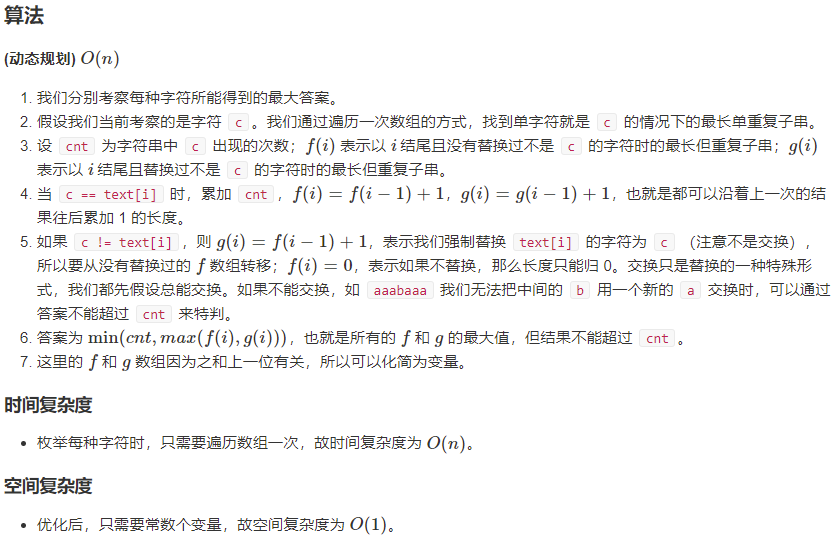
\includegraphics[width=.9\linewidth]{./pic/ssrepeat.png}
\end{itemize}
\begin{minted}[frame=lines,fontsize=\scriptsize,linenos=false]{java}
private int solve(char c, String s) {
    int n = s.length(), max = 0;
    int f = 0, g = 0, cnt = 0;
    for (int i = 0; i < n; i++) {
        if (c == s.charAt(i)) {
            f++;
            g++;
            cnt++;
        } else {
            g = f + 1;
            f = 0;
        }
        max = Math.max(max, Math.max(f, g));
    }
    return Math.min(max, cnt);
}
public int maxRepOpt1(String s) {
    int n = s.length(), ans = 0;
    for (char i = 'a'; i <= 'z'; i++) 
        ans = Math.max(ans, solve(i, s));
    return ans;
}
\end{minted}

\section{395. Longest Substring with At Least K Repeating Characters - Medium}
\label{sec-6-6}
Given a string s and an integer k, return the length of the longest substring of s such that the frequency of each character in this substring is greater than or equal to k.
\begin{minted}[frame=lines,fontsize=\scriptsize,linenos=false]{java}
//         由于字母只有 26 个,而整型 mask 有 32 位,足够用了,
//         每一位代表一个字母,如果为1,表示该字母不够k次,如果为0就表示已经出现了k次,这种思路真是太聪明了,
//         隐约记得这种用法在之前的题目中也用过,但是博主并不能举一反三( 沮丧脸:( ),还得继续努力啊。
// 遍历字符串,对于每一个字符,都将其视为起点,然后遍历到末尾,增加 HashMap 中字母的出现次数,如果其小于k,将 mask 的对应位改为1,如果大于等于k,将 mask 对应位改为0。
// 然后看 mask 是否为0,是的话就更新 res 结果,然后把当前满足要求的子字符串的起始位置j保存到 max_idx 中,等内层循环结束后,将外层循环变量i赋值为 max_idx+1,继续循环直至结束
public int longestSubstring(String s, int k) { // O (N ^ 2)
    int n = s.length(), res = 0, i = 0;
    while (i + k <= n) {
        int [] m = new int [26];
        int mask = 0, maxIdx = i;
        for (int j = i; j < n; j++) {
            int t = s.charAt(j) - 'a';
            m[t]++;
            if (m[t] < k) mask |= (1 << t);
            else mask &= (~(1 << t));
            if (mask == 0) {
                res = Math.max(res, j-i+1);
                maxIdx = j;
            }
        }
        i = maxIdx + 1;
    }
    return res;
}
\end{minted}
\begin{itemize}
\item 双指针sliding window O(N)
\end{itemize}
\begin{minted}[frame=lines,fontsize=\scriptsize,linenos=false]{java}
public int longestSubstring(String s, int k) {
    int n = s.length(), res = 0;
    for (int cnt = 1; cnt <= 26; cnt++) {
        int start = 0, i = 0, uniqueCnt = 0;
        int [] charCnt = new int [26];
        while (i < n) {
            boolean valid = true;
            if (charCnt[s.charAt(i++)-'a']++ == 0) ++ uniqueCnt;
            while (uniqueCnt > cnt) 
                if (--charCnt[s.charAt(start++)-'a'] == 0) --uniqueCnt;
            for (int j = 0; j < 26; j++)
                if (charCnt[j] > 0 && charCnt[j] < k) valid = false;
            if (valid) res = Math.max(res, i-start);
        }
    }
    return res;
}
\end{minted}
\begin{itemize}
\item 分治: 分而治之
\end{itemize}
\begin{minted}[frame=lines,fontsize=\scriptsize,linenos=false]{java}
public int longestSubstring(String s, int k) { // str.split("[dkfldjf]")
    int n = s.length();
    if (n < k) return 0;
    if (n == k && s.chars().distinct().count() == 1) return k;
    int [] cnt = new int [26];
    for (int i = 0; i < n; i++) 
        cnt[s.charAt(i)-'a']++;
    if (Arrays.stream(cnt).max().getAsInt() < k) return 0;
    StringBuilder sb = new StringBuilder("[");
    for (int i = 0; i < 26; i++) 
        if (cnt[i] < k && cnt[i] != 0)
            sb.append((char)(i+'a'));
    sb.append(']');
    if (sb.length() == 2) return n;
    String [] sa = s.split(sb.toString()); // str.split("[-+*/=]") pay attention to the format
    System.out.println(Arrays.toString(sa));
    int max = 0;
    for (int i = 0; i < sa.length; i++) 
        max = Math.max(max, longestSubstring(sa[i], k));
    return max;
}
public int longestSubstring(String s, int k) { // 人工手动折分
    int n = s.length(), maxIdx = 0, res = 0;
    int [] cnt = new int [128];
    boolean valid = true;
    for (char c : s.toCharArray()) 
        cnt[c]++;
    for (int i = 0; i < n; i++) 
        if (cnt[s.charAt(i)] < k) {
            res = Math.max(res, longestSubstring(s.substring(maxIdx, i), k));
            valid = false;
            maxIdx = i+1;
        }
    return valid ? n : Math.max(res, longestSubstring(s.substring(maxIdx, n), k));
}
\end{minted}

\chapter{Segment Tree与Binary Index Tree 线段树与树状数组}
\label{sec-7}

线段树(segment tree),顾名思义, 是用来存放给定区间(segment, or interval)内对应信息的一种数据结构。与树状数组(binary indexed tree)相似,线段树也用来处理数组相应的区间查询(range query)和元素更新(update)操作。与树状数组不同的是,线段树不止可以适用于区间求和的查询,也可以进行区间最大值,区间最小值(Range Minimum/Maximum Query problem)或者区间异或值的查询。

对应于树状数组,线段树进行更新(update)的操作为O(logn),进行区间查询(range query)的操作也为O(logn)。

\section{1157. Online Majority Element In Subarray - Hard}
\label{sec-7-1}
Design a data structure that efficiently finds the majority element of a given subarray.

The majority element of a subarray is an element that occurs threshold times or more in the subarray.

Implementing the MajorityChecker class:

MajorityChecker(int[] arr) Initializes the instance of the class with the given array arr.
int query(int left, int right, int threshold) returns the element in the subarray arr[left\ldots{}right] that occurs at least threshold times, or -1 if no such element exists.
\begin{minted}[frame=lines,fontsize=\scriptsize,linenos=false]{java}
private class Node {
    private int bgn;
    private int end;
    private int val;
    private int cnt; // sum
    private Node left;
    private Node right;
    public Node(int bgn, int end, int val, int cnt) {
        this.bgn = bgn;
        this.end = end;
        this.val = val;
        this.cnt = cnt;
        this.left = null;
        this.right = null;
    }
    public Node(int bgn, int end, int val, int cnt, Node left, Node right) {
        this.bgn = bgn;
        this.end = end;
        this.val = val;
        this.cnt = cnt;
        this.left = left;
        this.right = right;
    }
}
public void update(int index, int val) {
    updateTree(root, index, val);
}
public int cntRange(int left, int right) {
    return cntRangeFromTree(root, left, right);
}
private int cntRangeFromTree(Node r, int i, int j) {
    if (r == null || i < r.bgn || i > r.end) return 0;
    else if (i <= r.bgn && j >= r.end) return r.cnt;
    else return cntRangeFromTree(r.left, i, j) + cntRangeFromTree(r.right, i, j);
}
private void updateTree(Node r, int i, int va) {
    if (r == null || i < r.bgn || i > r.end) return;
    else if (r.bgn == r.end && r.bgn == i) r.cnt = va; 
    else {
        updateTree(r.left, i, va);
        updateTree(r.right, i, va);
        int cnt = 0;
        if (r.left != null) cnt += r.left.cnt;
        if (r.right != null) cnt += r.right.cnt;
        r.cnt = cnt;
    }
}
private Node buildTree(int [] arr, int i, int j) { 
    if (i > j) return null;
    else if (i == j)
        return new Node(i, i, arr[i], 1);
    else {
        int mid = i + (j-i)/2;
        Node left = buildTree(arr, i, mid);
        Node right = buildTree(arr, mid+1, j);
        if (left.val == right.val)
            return new Node(i, j, left.val, left.cnt + right.cnt, left, right);
        else {
            if (left.cnt > right.cnt)
                return new Node(i, j, left.val, left.cnt-right.cnt, left, right);
            else return new Node(i, j, right.val, right.cnt-left.cnt, left, right);
        }
    }
}
// 排序数组中 第一个大于tar的下标
int upper_bound(List<Integer> list, int tar) {
    int l = 0, r = list.size();
    while (l < r) {
        int mid = l + (r-l)/2;
        if (list.get(mid) <= tar) l = mid+1;
        else r = mid;
    }
    return l;
}
// 排序数组中 第一个大于等于tar的下标
int lower_bound(List<Integer> list, int tar) {
    int l = 0, r = list.size()-1;
    while (l < r) {
        int mid = l + (r-l)/2;
        if (list.get(mid) < tar) l = mid+1;
        else r = mid;
    }
    return l;
}
/**
 * 构建线段树
 * @param arr 被构建数组
 * @param l 构建节点的左值 表示查询区域左边界
 * @param r 构建节点的右值 表示查询区域右边界
 * @return 以构建完成的线段树节点
 * */
private SegTreeNode buildTree(int[] arr, int l, int r) {
    if (l > r) return null;
    // 初始一个线段树节点
    SegTreeNode root = new SegTreeNode(l, r);
    // 叶子节点
    if (l == r) {
        // 众数就是当前值 计数为1
        root.val = arr[l]; root.count = 1;
        return root;
    }

    int mid = (l+r)/2;
    // 构建左子节点
    root.left = buildTree(arr, l, mid);
    // 构建右子节点
    root.right = buildTree(arr, mid+1, r);
    // 整合父节点
    makeRoot(root);
    return root;
}
/**
 * 整合一个父节点
 * @param root 被整合节点
 * */
private void makeRoot(SegTreeNode root) {
    if (null == root) return;
    // 如果该节点有左子节点 该节点的值"先"等于左子节点
    if (root.left != null) {
        root.val = root.left.val;
        root.count = root.left.count;
    }
    // 如果该节点还有右子节点 融合父节点和子节点
    if (root.right != null) {
        if (root.val == root.right.val) 
            root.count = root.count + root.right.count;
        else {
            if (root.count >= root.right.count) 
                root.count = root.count - root.right.count;
            else {
                root.val = root.right.val; 
                root.count = root.right.count - root.count;
            }
        }
    }
}    
/**
 * 查询线段树
 * @param root 被查询节点
 * @param l 需要查询的范围左边界
 * @param r 需要查询的范围右边界
 * */
private void searchSegTree(Node root, int l, int r) {
    if (root == null || l > r) return;
    if (root.bgn > r || root.end < l) return;

    // 当查询边界 覆盖 节点边界 该节点就是查询区域
    if (root.bgn >= l && root.end <= r) {
        if (key == root.val) cnt += root.cnt;
        else if (cnt <= root.cnt) {
            key = root.val;
            cnt = root.cnt - cnt;
        } else cnt = cnt - root.cnt;
        return;
    }

    int mid = (root.end + root.bgn)/2;
    // root.bgn <= l <= mid 左节点也可以是查询区域
    if (l <= mid)  // 这两个查询条件再好好想想 !!!!!!!!!!!!!!!
        searchSegTree(root.left, l, r);
    // mid+1 <= r <= root.end 右节点也可以是查询区域
    if (r >= mid+1) 
        searchSegTree(root.right, l, r);
}
// https://books.halfrost.com/leetcode/ChapterFour/1100~1199/1157.Online-Majority-Element-In-Subarray/ 也有一个直观图
// https://www.cnblogs.com/slowbirdoflsh/p/11381565.html 思路比较清晰
HashMap<Integer, List<Integer>> idx = new HashMap<>();
private Node root;
int key = 0, cnt = 0;
public MajorityChecker(int[] arr) {
    root = buildTree(arr, 0, arr.length-1);
    levelPrintTree(root);
    idx = new HashMap<>();
    for (int i = 0; i < arr.length; i++) {
        if (!idx.containsKey(arr[i]))
            idx.put(arr[i], new ArrayList<>());
        idx.get(arr[i]).add(i);
    }
}
public int countRangeSum(int[] nums, int lower, int upper) {
    MajorityChecker mc = new MajorityChecker(nums);
}
public int query(int left, int right, int threshold) {
    // 初始化 所查询众数key 及辅助判断的计数cnt
    key = 0; cnt = 0;
    // 查询线段树
    searchSegTree(root, left, right);
    // 如果查询区域没有众数 即key没被更改
    // 或者
    // 所查询出来的众数 在原数组中根本没有超出阈值的能力
    System.out.println("key: " + key);
    System.out.println("(idx.get(key) == null): " + (idx.get(key) == null));

    if (key == 0 || idx.get(key).size() < threshold) return -1;

    // 上确界 排序数组中 第一个大于right的下标
    int r = upper_bound(idx.get(key), right);
    // 下确界 排序数组中 第一个大于等于left的下标
    int l = lower_bound(idx.get(key), left);
    cnt = r - l;
    return cnt >= threshold ? key : -1;
}
\end{minted}

\section{1825. Finding MK Average - Hard}
\label{sec-7-2}
You are given two integers, m and k, and a stream of integers. You are tasked to implement a data structure that calculates the MKAverage for the stream.

The MKAverage can be calculated using these steps:

If the number of the elements in the stream is less than m you should consider the MKAverage to be -1. Otherwise, copy the last m elements of the stream to a separate container.
Remove the smallest k elements and the largest k elements from the container.
Calculate the average value for the rest of the elements rounded down to the nearest integer.
Implement the MKAverage class:

MKAverage(int m, int k) Initializes the MKAverage object with an empty stream and the two integers m and k.
void addElement(int num) Inserts a new element num into the stream.
int calculateMKAverage() Calculates and returns the MKAverage for the current stream rounded down to the nearest integer.
\begin{minted}[frame=lines,fontsize=\scriptsize,linenos=false]{java}
// 根据题意需要找到前k大的数,又需要求区间和,就自然想到线段树.写起来较不容易出错。
// 维护2个线段树数组,一个记录数的个数,一个记录区间值,
// 注意一般线段树中[s,e]指固定的区间,这里类似线段数求第k小的数,所以[s,e]指第s小的值到第e小的值的区间。
LinkedList<Integer> q;
int [] cnt;
long[] sum;
int m,k;
public MKAverage(int m, int k) {
    q = new LinkedList<>();
    cnt = new int[400001]; // space: 4N
    sum = new long[400001];
    this.m = m;
    this.k = k;
}
public void addElement(int num) {
    if (q.size() == m) {
        int v = q.pollFirst();
        insert(1, 0, 100000, v, -1);
    }
    insert(1, 0, 100000, num, 1);
    q.addLast(num);
}
public int calculateMKAverage() {
    if (q.size() < m)return -1;
    int s = k+1, e = m-k;
    return (int)(query(1, 0, 100000, s, e)/(m-2*k));
}
void insert(int idx, int l, int r, int v, long d) {
    cnt[idx] += d;
    sum[idx] += d*v;
    if (l == r) return;
    int m = l + (r-l)/2;
    if (v <= m)
        insert(idx<<1, l, m, v, d);    // 向左子树查询
    else
        insert(idx<<1|1, m+1, r, v, d);// 向右子树查询
}
long query(int idx, int l, int r, int s, int e){//线段中第s个到第e个
    if (l == r) {//起始和结束最多出现2次此情况
        int c = e-s+1;
        return (long)c*l;
    } else if (cnt[idx] == e-s+1) {
        return sum[idx];
    } else {
        int m = (l+r)/2;
        int c1 = cnt[idx<<1];
        int c2 = cnt[idx<<1|1];
        if (c1 >= e){
            return query(idx<<1, l, m, s, e);
        } else if (c1 >= s){
            return query(idx<<1, l, m, s, c1)+query(idx<<1|1, m+1, r, 1, e-c1);
        } else {//c1<s
            return query(idx<<1|1, m+1, r, s-c1, e-c1);
        }
    }
}
\end{minted}
\begin{itemize}
\item 数状数组的解法: 另外第一次看到别人 二分+树状数组也能求前k大的值。
\end{itemize}
\begin{minted}[frame=lines,fontsize=\scriptsize,linenos=false]{java}
// We can have a queue to maintain m elements
// Use two Fenwick tree, 1 for count and 1 for prefix sum
// Do 2 times binary search for the first k elements and the last k elements by using the count from our first fenwick tree
// We can get the sum by subtrating the sum of first k elements and sum of last k element by using our second fenwick tree
Queue<Integer> q = new LinkedList<>();
FenWick fone, ftwo;
int [] cnt = new int [100010];
long sum = 0;
int m,k;
public MKAverage(int m, int k) {
    this.m = m;
    this.k = k;
    long A [] = new long [100010];
    long B [] = new long [100010];
    fone = new FenWick(A);
    ftwo = new FenWick(B);
}
public void addElement(int num) {
    q.add(num);
    sum += num;
    fone.update(num, 1);
    ftwo.update(num, num);
    cnt[num]++;
}
public int calculateMKAverage() {
    if (q.size() < m) return -1;
    while (q.size() > m) {
        int cur = q.poll();
        cnt[cur]--;
        sum -= cur;
        fone.update(cur, -1);
        ftwo.update(cur, -cur);
    }
    // binary search for the first k (there may be duplicated)
    int l = 0, r = cnt.length-1;
    int i = -1, j = -1; // pos1, pos2 
    while (l <= r) { // 二分查找总计数
        int m = (r + l) / 2;
        long count = fone.sumRange(0, m);
        if (count >= k) {
            i = m;
            r = m -1;
        } else l = m+1;
    }
    // binary search for the last k (there may be duplicated)
    l = 0;
    r = cnt.length-1;
    while (l <= r) {
        int m = l + (r-l)/2;
        long count = fone.sumRange(m, cnt.length-1);
        if (count >= k) {
            j = m;
            l = m + 1;
        } else r = m-1;
    }
    long sum1 = ftwo.sumRange(0,  i);
    long sum2 = ftwo.sumRange(j, cnt.length-1);
    long cnt1 = fone.sumRange(0, i);
    long cnt2 = fone.sumRange(j, cnt.length-1);
    if (cnt1 > k)
        sum1 -= i*(cnt1-k);
    if (cnt2 > k)
        sum2 -= j*(cnt2-k);
    long remain = sum - sum1 - sum2; // 总和, 减去两边最小最大各K个数的和
    return (int)(remain / (m-2*k));
}
class FenWick {
    long tree []; //1-index based
    long A [];
    long arr[];
    public FenWick(long [] A) {
        this.A = A;
        arr = new long [A.length];
        tree = new long [A.length + 1];
    }
    public void update(int i, int v) {
        arr[i] += v;
        i++;
        while (i < tree.length) {
            tree[i] += v;
            i += (i & -i); // 这是的原理细节再回去复习一下
        }
    }
    public long sumRange(int i, int j) {
        return pre(j+1)-pre(i);
    }
    public long pre(int i) {
        long sum = 0;
        while (i > 0) {
            sum += tree[i];
            i -= (i & -i);
        }
        return sum;
    }
}
\end{minted}

\chapter{树结构:各种新型数据结构}
\label{sec-8}

\section{968. Binary Tree Cameras}
\label{sec-8-1}
You are given the root of a binary tree. We install cameras on the tree nodes where each camera at a node can monitor its parent, itself, and its immediate children.
Return the minimum number of cameras needed to monitor all nodes of the tree.
\begin{minted}[frame=lines,fontsize=\scriptsize,linenos=false]{java}
// 对于每个节点,有一下三种case:
// case(1):如果它有一个孩子,且这个孩子是叶子(状态0),则它需要摄像头,res ++,然后返回1,表示已经给它装上了摄像头。
// case(2):如果它有一个孩子,且这个孩子是叶子的父节点(状态1),那么它已经被覆盖,返回2。
// case(0):否则,这个节点无孩子,或者说,孩子都是状态2,那么我们将这个节点视为叶子来处理。
// 由于dfs最终返回后,整棵树的根节点的状态还未处理,因此需要判断,若根节点被视为叶子,需要在其上加一个摄像头。
private int dfs(TreeNode r) {
    // 空节点不需要被覆盖,归入情况2
    if (r == null) return 2; // do not need cover
    int left = dfs(r.left);  // 递归求左右孩子的状态
    int right = dfs(r.right);
    // 获取左右孩子状态之后的处理
    // 有叶子孩子,加摄像头,归入情况1
    if (left == 0 || right == 0) {
        res ++;
        return 1;
    }
    // 孩子上有摄像头,说明此节点已被覆盖,情况2; 
    if (left == 1 || right == 1) return 2;
    return 0;
}
int res = 0;
public int minCameraCover(TreeNode root) {
    // 若根节点被视为叶子,需要在其上加一个摄像头
    return (dfs(root) == 0 ? 1 : 0) + res;
}
\end{minted}
\section{1696. Jump Game VI}
\label{sec-8-2}
You are given a 0-indexed integer array nums and an integer k.
You are initially standing at index 0. In one move, you can jump at most k steps forward without going outside the boundaries of the array. That is, you can jump from index i to any index in the range [i + 1, min(n - 1, i + k)] inclusive.
You want to reach the last index of the array (index n - 1). Your score is the sum of all nums[j] for each index j you visited in the array.
Return the maximum score you can get.
\begin{minted}[frame=lines,fontsize=\scriptsize,linenos=false]{java}
public int maxResult(int[] nums, int k) { // O(N) DP with double ended queue
    int n = nums.length;
    int [] dp = new int[n];
    ArrayDeque<Integer> q = new ArrayDeque<>();
    for (int i = 0; i < n; i++) {
        while (!q.isEmpty() && q.peekFirst() < i-k) // 头大尾小
            q.removeFirst();
        dp[i] = nums[i] + (q.isEmpty() ? 0 : dp[q.peekFirst()]);
        while (q.size() > 0 && dp[q.peekLast()] <= dp[i])
            q.removeLast();
        q.addLast(i);
    }
    return dp[n-1];
}
public int maxResult(int[] nums, int k) { // BigO: O (NlogN)
    int n = nums.length;
    int [] dp = new int[n];
    Queue<int []> q = new PriorityQueue<>(Comparator.comparingInt(e -> -e[0]));
    for (int i = 0; i < n; i++) {
        while (!q.isEmpty() && q.peek()[1] + k < i)
            q.poll();
        dp[i] = nums[i] + (q.isEmpty() ? 0 : q.peek()[0]);
        q.add(new int[] {dp[i], i});
    }
    return dp[n-1];
}
\end{minted}

\section{Create Sorted Array through Instructions}
\label{sec-8-3}
Given an integer array instructions, you are asked to create a sorted array from the elements in instructions. You start with an empty container nums. For each element from left to right in instructions, insert it into nums. The cost of each insertion is the minimum of the following:
The number of elements currently in nums that are strictly less than instructions[i].
The number of elements currently in nums that are strictly greater than instructions[i].
For example, if inserting element 3 into nums = [1,2,3,5], the cost of insertion is min(2, 1) (elements 1 and 2 are less than 3, element 5 is greater than 3) and nums will become [1,2,3,3,5].
Return the total cost to insert all elements from instructions into nums. Since the answer may be large, return it modulo 109 + 7
\begin{minted}[frame=lines,fontsize=\scriptsize,linenos=false]{java}
// https://blog.csdn.net/qq_28033719/article/details/112506925
private static int N = 100001;
private static int [] tree = new int [N]; // 拿元素值作为 key 对应 tree 的下标值
public int lowbit(int i) {
    return i & -i;
}
public void update(int i, int v) { // 更新父节点
    while (i <= N) {
        tree[i] += v;
        i += lowbit(i);
    }
}
public int getSum(int i) { // 得到以 i 为下标1-based的所有子、叶子节点的和, 也就是[1, i]的和,1-based
    int ans = 0;
    while (i > 0) {
        ans += tree[i];
        i -= lowbit(i);
    }
    return ans;
}
public int createSortedArray(int[] instructions) {
    int n = instructions.length;
    long res = 0;
    Arrays.fill(tree, 0);
    for (int i = 0; i < n; i++) {
        //              严格小于此数的个数 严格大于此数的个数: 为总个数(不含自己) - 小于自己的个数
        res += Math.min(getSum(instructions[i]-1), i-getSum(instructions[i])); 
        update(instructions[i], 1);
    }
    return (int)(res % ((int)Math.pow(10, 9) + 7));
}
\end{minted}

\section{1932. Merge BSTs to Create Single BST: 这颗树我曾投入巨大热情,可是总不过,好缺德}
\label{sec-8-4}
You are given n BST (binary search tree) root nodes for n separate BSTs stored in an array trees (0-indexed). Each BST in trees has at most 3 nodes, and no two roots have the same value. In one operation, you can:

Select two distinct indices i and j such that the value stored at one of the leaves of trees[i] is equal to the root value of trees[j].
Replace the leaf node in trees[i] with trees[j].
Remove trees[j] from trees.
Return the root of the resulting BST if it is possible to form a valid BST after performing n - 1 operations, or null if it is impossible to create a valid BST.

A BST (binary search tree) is a binary tree where each node satisfies the following property:

Every node in the node's left subtree has a value strictly less than the node's value.
Every node in the node's right subtree has a value strictly greater than the node's value.
A leaf is a node that has no children.
\begin{minted}[frame=lines,fontsize=\scriptsize,linenos=false]{java}
public TreeNode canMerge(List<TreeNode> trees) {
    final int size = trees.size();
    final Map<Integer, TreeNode> roots = new HashMap<>(size);
    for (final TreeNode node : trees) 
        roots.put(node.val, node);
    for (final TreeNode node : trees) {
        if (roots.containsKey(node.val)) { // 这里判断:是因为接下来buildTree会将可以合并的子树键值对删除并回收利用建大树了
            final TreeNode root = buildTree(roots, node);
            roots.put(root.val, root);    // update root node
        }
    }
    if (roots.size() != 1) return null;   // 无法合并所有的子树
    final TreeNode root = roots.values().iterator().next(); // 只有这一颗树根
    return isValid(root, Integer.MIN_VALUE, Integer.MAX_VALUE) ? root : null;
}
private TreeNode buildTree(Map<Integer, TreeNode> roots, TreeNode node) { // 用recursion把所有需要/可以合并的子树建成一棵完整大树,方法很传神
    final TreeNode next = roots.remove(node.val); // map.remove()返回值: 如果存在key, 则删除并返回value;如果不存在则返回null
    if (next != null) {
        if (next.left != null) node.left = buildTree(roots, next.left);
        if (next.right != null) node.right = buildTree(roots, next.right);
    }
    return node;
}
private boolean isValid(TreeNode node, int min, int max) { // 这些个递归写得很传功力,要活学活用到出神入化。。。。。。
    if (node == null) return true;
    final int value = node.val;
    if (value <= min || value >= max) return false;
    return isValid(node.left, min, value) && isValid(node.right, value, max);
}
\end{minted}

\chapter{Trie}
\label{sec-9}
应用
Trie树最直观的定义就是LinkedList of HashMap。所以Trie和HashMap都可以用来查询某个单词是否在字典当中。我们需要知道他们的优缺点。
优点:
支持字符级别的查询,比如说我们需要在matrix当中通过traverse构造单词,那么这个单词是一个一个字符形成的,我们可以在traverse的每一步去检验当前路径是否可以形成valid word。另外,对于含有regex符号的字符串,我们需要一个字符一个字符的考虑,这种情况下我们也需要通过trie去查找。
节省空间,相同的prefix只存一遍,而HashMap需要存很多遍。
缺点:实现起来较麻烦,大部分题目使用Trie都是overkill,所以除非需要支持字符级别的查询,否则HashMap更好。
操作: 三个操作:
insert
search
startWith
其中insert记得把最后一个node标记为isEnd = true。其中search和startWith都可以通过同一个searchHelper helper method来实现,我们只需要return 最后一个node就可以,如果isEnd == true,那么说明找到一个完整的单词,否则至少找到了prefix。别忘了使用trie的第一步是preprocess,把字典里的所有word加入到trie树当中。
题目
\section{208. Implement Trie (Prefix Tree)}
\label{sec-9-1}
\section{212. Word Search II}
\label{sec-9-2}
\section{211. Add and Search Word - Data structure design (Facebook店面)}
\label{sec-9-3}
\section{14. Longest Common Prefix (这道题可以稍作改编,比如说string list会经常update,会经常query,那这时很明显用trie更好)}
\label{sec-9-4}
\section{421. Maximum XOR of Two Numbers in an Array}
\label{sec-9-5}
Given an integer array nums, return the maximum result of nums[i] XOR nums[j], where 0 <= i <= j < n.

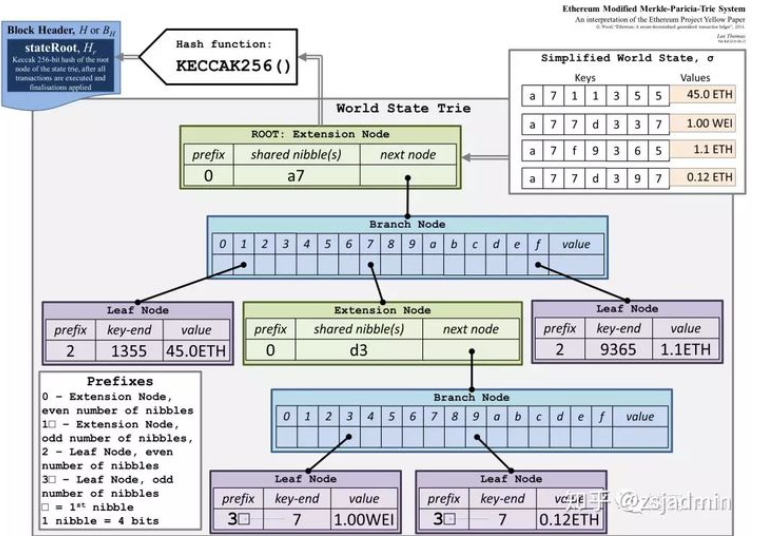
\includegraphics[width=.9\linewidth]{./pic/numTrie.png}

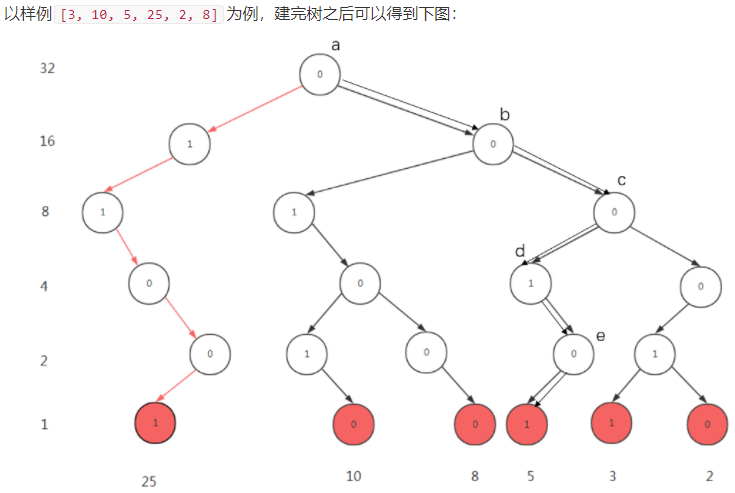
\includegraphics[width=.9\linewidth]{./pic/numTrie2.png}

左儿子为1的分支,右儿子为0的分支。

然后依次枚举每个数,在Trie树中找到与它异或结果最大的数。

这一步可以贪心来做:

从高位到低位,依次在Trie树中遍历,每次尽量走到与当前位不同的分支,这样可以使得找到的数与当前数在当前二进制位的异或结果是1,从而可以得到尽量大的结果。

如上图所示,我们用25来举例说明,它的二进制表示是(11001):

\begin{minted}[frame=lines,fontsize=\scriptsize,linenos=false]{java}
最初指针在根节点(编号是a的点),我们从25的二进制表示的最高位开始枚举;
  由于最高位是1,我们走到0分支,走到b点;
  次高位是1,我们继续往右儿子走,走到c点;
  下一位是0,我们往左走,走到d点;
  下一位是0,我们希望往左走,但发现左儿子不存在,所以只能往右走,走到e点;
  最后一位是1,我们希望往右走,但发现右儿子不存在,所以只能往左走,最终走到5;
所以和25异或值最大的数是5, 25 ^ 5 = 28。
\end{minted}
\begin{minted}[frame=lines,fontsize=\scriptsize,linenos=false]{java}
public class Trie {
    private class Node { // 这我自己写的乱代码,贴在这里很不相关,也需要先测试一下
        public int val;
        public boolean isExist;
        public Node [] next;
        public Node(boolean isExist) {
            this.isExist = isExist;
            next = new Node[2];
            val = 0;
        }
        public Node() { this(false); }
        public Node(int va) {
            this(true);
            this.val = va;
        }
    }
    private Node root;
    public Trie() { root = new Node(); }
    public void insert(int va) {
        Node cur = root;
        for (int i = 31; i >= 0; i--) {
            int tmp = (va >> i) & 1;
            if (cur.next[tmp] == null)
                cur.next[tmp] = new Node();
            cur = cur.next[tmp];
        }
        cur.isExist = true;
    }
    public int search(int va) {
        int max = 0;
        Node cur = root;
        for (int i = 31; i >= 0; i--) {
            int t = (va >> i) & 1;
            if (cur.next[t^1] != null) {
                max += (1 << i);
                cur = cur.next[t^1];
            } else cur = cur.next[t&1];
        }
        return max;
    }
}
\end{minted}

\subsection{另一种位操作法}
\label{sec-9-5-1}

\begin{itemize}
\item 学到了异或操作的一个重要性质:a$^{\text{b}}$ = c, 则有 a$^{\text{c}}$ = b,且 b$^{\text{c}}$ = a;
\end{itemize}

我们还需要用上一个异或的特性,假设a和b产生了最终的答案max,即a \^{} b = x,那么根据异或的特性,a \^{} x = b。同理,a和b的最高位(前n位)也有相同的性质。

先以最高位为例子,我们可以把所有的数字的最高位放到一个HashSet里面,然后使用1与set里面的所有数字进行异或,如果得出的结果仍然在set里面,那么最终结果的最高位必然为1,否则为0。也即,先假定结果为1,然后与set中所有数字异或,假定a与1异或得到结果b(a \^{} 1 = b),而b仍然在set里面,那么说明set中有两个数字异或能得到1(a \^{} b = 1)。否则,set中没有两个数字能够异或得到1,那么最终结果的最高位为1的假设失败,说明最终结果的最高位为0。以此类推可以得到第二位、第三位。。。的数字。

再做一下推广,我们将所有数字的前N位放到一个HashSet里面,然后使用之前N-1位得到的最大值前缀prefix与set里面的所有数字进行异或,如果得出的结果仍然在set中,那么第N位必然为1,否则为0。

举个例子,给定数组[14, 11, 7, 2],二进制表示分别为[1110, 1011, 0111, 0010]。题目说了,数字最长不会超过32位,所以应从i = 31开始,但是所有数字中最多位4位数,简单起见,我直接从最高位i=3开始
\begin{minted}[frame=lines,fontsize=\scriptsize,linenos=false]{java}
[14,   11,   7,    2]
[1110, 1011, 0111, 0010]
1. i = 3, set = {1000, 0000} => max = 1000
2. i = 2, set = {1100, 1000, 0100, 0000} => max = 1100
3. i = 1, set = {1110, 1010, 0110, 0010} => max = 1100
4. i = 0, set = {1110, 1011, 0111, 0010} => max = 1100
\end{minted}
\begin{minted}[frame=lines,fontsize=\scriptsize,linenos=false]{java}
public int findMaximumXOR(int[] nums) { // 这种解法没有用到上面的这个trie呀
    int n = nums.length;
    int mask = 0, max = 0;
    HashSet<Integer> s = new HashSet<>();
    for (int i = 31; i >= 0; --i) { // i == 31时
        mask = mask | 1 << i;     // 为获取前n位的临时变量     
        for (int va : nums) 
            s.add(va & mask);     // 将所有数字的前n位放入set中
        int tmp = max | (1 << i); // 假定第n位为1,前n-1位max为之前迭代求得
        for (Integer va : s) 
            if (s.contains(va ^ tmp)) { // 查看`b`是否在 // i == 31, (va^tmp):  -2147483648
                max = tmp;              // b存在,第n位为1
                break;
            }
        s.clear();
    }
    return max;
}
// 此解法时间复杂度为O(32n)=O(n),空间复杂度上,我们使用了一个HashSet用于存储所有数字,因此空间复杂度是O(n)
\end{minted}

\section{1617. Count Subtrees With Max Distance Between Cities - Hard}
\label{sec-9-6}
There are n cities numbered from 1 to n. You are given an array edges of size n-1, where edges[i] = [ui, vi] represents a bidirectional edge between cities ui and vi. There exists a unique path between each pair of cities. In other words, the cities form a tree.

A subtree is a subset of cities where every city is reachable from every other city in the subset, where the path between each pair passes through only the cities from the subset. Two subtrees are different if there is a city in one subtree that is not present in the other.

For each d from 1 to n-1, find the number of subtrees in which the maximum distance between any two cities in the subtree is equal to d.

Return an array of size n-1 where the dth element (1-indexed) is the number of subtrees in which the maximum distance between any two cities is equal to d.

Notice that the distance between the two cities is the number of edges in the path between them.
\begin{itemize}
\item So apparently the brute-force approach passed this question. I guess for future contests, I should really pay attention to the input size\ldots{}
\end{itemize}
\begin{minted}[frame=lines,fontsize=\scriptsize,linenos=false]{java}
public int [] countSubgraphsForEachDiameter(int n, int[][] edges) {
    int [] res = new int [n-1];
    List<List<int []>> subsets = new ArrayList<>();
    generateSubsets(edges, new ArrayList<int []>(), subsets, 0);
    for (List<int []> subset : subsets) 
        solve(subset, res);
    return res;
}
private void solve(List<int []> subset, int [] res) {
    if (!isValidGraph(subset)) return;
    Map<Integer, List<Integer>> graph = new HashMap<>();
    for (int [] eg : subset) {
        graph.computeIfAbsent(eg[0], k -> new ArrayList<>()).add(eg[1]);
        graph.computeIfAbsent(eg[1], k -> new ArrayList<>()).add(eg[0]);
    }
    int max = 1;
    for (Integer key : graph.keySet()) {
        if (graph.get(key).size() == 1) {
            int [] longest = new int [] {1}; // 减少global变量的数量
            Set<Integer> vis = new HashSet<>();
            vis.add(key);
            dfs(graph, vis, key, longest, 0);
            max = Math.max(max, longest[0]);
        }
    }
    res[max - 1]++;
}
private void dfs(Map<Integer, List<Integer>> graph, Set<Integer> vis, int idx, int [] longest, int level) {
    longest[0] = Math.max(longest[0], level);
    for (Integer node : graph.get(idx)) 
        if (vis.add(node)) // Set.add(element) return false if it contains element already
            dfs(graph, vis, node, longest, level + 1);
}
private boolean isValidGraph(List<int []> subset) {
    Set<Integer> nodes = new HashSet<>();
    for (int [] cur : subset) {
        nodes.add(cur[0]);
        nodes.add(cur[1]);
    }
    return nodes.size() - 1 <= subset.size();
}
private void generateSubsets(int [][] arr, List<int []> cur, List<List<int []>> res, int idx) {
    if (idx == arr.length) return; // arr.length <= 15, 用回塑法直接生成subsets,但是这是相对耗时的操作
    for (int i = idx; i < arr.length; i++) {
        cur.add(arr[i]);
        res.add(new ArrayList<>(cur));
        generateSubsets(arr, cur, res, i+1);
        cur.remove(cur.size()-1);
    }
}
\end{minted}
\begin{itemize}
\item 另一种位操作法
\end{itemize}
\begin{minted}[frame=lines,fontsize=\scriptsize,linenos=false]{java}
// One way in which we can find the diameter of a tree is using DFS, just like if our tree is represented using tree nodes instead of as grpah
//     1. Make a call to DFS from any node as root, lets say 1 as root
//     2. Maintain a global max parameter
//     3. For each call to dfs, of all current node's children (excluding parent)
//        find top two distances from current node to any leaf reachable from current node
//     4. Sum of these top two distances froms the longes path passing through current node to all its children. Update if this path is maximum
//     5. return 1 + top distance for this dfs call. Need to add 1 since,
//        max length of path that can be reached from current ndoe is current ndoe + max distance reachable from current ndoes's children
int ans = 0, vis = 0;
int [] res;
public int [] countSubgraphsForEachDiameter(int n, int[][] edges) {
    res = new int [n-1];
    ans = 0; vis = 0;
    Map<Integer, List<Integer>> graph = new HashMap<>();
    for (int [] i : edges) { // if our node is 5, we store it as 1 << 4 which is 2^4
        graph.computeIfAbsent(1 << (i[0]-1), ArrayList::new).add(1 << (i[1]-1));
        graph.computeIfAbsent(1 << (i[1]-1), ArrayList::new).add(1 << (i[0]-1));
    }
    int range = (1 << n) - 1;  // (int)Math.pow(2, n) - 1;
    for (int subset = 3; subset <= range; subset++) {
        boolean isPowerOf2 = subset != 0 && (subset & (subset - 1)) == 0; // is power of 2
        if (isPowerOf2) continue;      // Single node subtrees can be excluded.
        ans = 0; vis = 0;
        dfs(graph, subset, Integer.highestOneBit(subset), -1); // Integer.highestOneBit(subset): subset: 0b1100, highest: 0b1000
        if (vis == subset)   // If visited is not equal to our current subset, all nodes are not reachable.
            res[ans - 1] ++; // In otherwords is not a proper subtree, hence dont include in the answer
    }
    return res;
}
// we can pass any node in this subset as root for dfs, we are passing node represented with highest set bit as root
// pass -1 as parent of root, since it has no root
private int dfs(Map<Integer, List<Integer>> graph, int subset, int cur, int pre) {
    if ((subset & cur) == 0) return 0;
    vis = vis | cur; 
    int fstMax = 0, sndMax = 0;
    for (Integer next : graph.get(cur)) {
        if (next == pre) continue;
        int dist = dfs(graph, subset, next, cur);
        if (dist > fstMax) {
            sndMax = fstMax;
            fstMax = dist;
        } else sndMax = Math.max(sndMax, dist);
    }
    ans = Math.max(ans, fstMax + sndMax); // top two distances from this node c
// top distance this cur node to any leaf is topdistance from c's children + 1. Adding 1 since we need to include cur node
    return 1 + fstMax; // 这里要再想一下 ???
}
\end{minted}

\section{1938. Maximum Genetic Difference Query - Hard 离线算法、离线思维、批量处理、顺序无关}
\label{sec-9-7}
There is a rooted tree consisting of n nodes numbered 0 to n - 1. Each node's number denotes its unique genetic value (i.e. the genetic value of node x is x). The genetic difference between two genetic values is defined as the bitwise-XOR of their values. You are given the integer array parents, where parents[i] is the parent for node i. If node x is the root of the tree, then parents[x] == -1.

You are also given the array queries where queries[i] = [nodei, vali]. For each query i, find the maximum genetic difference between vali and pi, where pi is the genetic value of any node that is on the path between nodei and the root (including nodei and the root). More formally, you want to maximize vali XOR pi.

Return an array ans where ans[i] is the answer to the ith query.
\begin{minted}[frame=lines,fontsize=\scriptsize,linenos=false]{java}
// 可以从根节点开始,对整棵树进行一次深度优先遍历,即:
// 当我们第一次遍历到某一节点 ii 时,我们将 ii 放入「数据结构」中;
// 当我们遍历完所有节点 ii 的子节点,即将回溯到 ii 的父节点前,我们将 ii 从「数据结构」中移除。
// 这样一来,我们就可以通过「离线」的思想将每一个询问在遍历到节点 \textit{val}_ival 时进行求解。这是因为,如果当前正在遍历节点 \textit{val}_ival
// 那么数据结构中就存放着所有从根节点到节点 \textit{val}_ival 的路径上的所有节点。
// 此时,我们只需要找出数据结构中使得 p_i \oplus \textit{val}_ip 达到最大值的节点 p_ip 即可。
// 而深度优先搜索过程中,当前入队的部分正是该节点及其所有层级的父节点,因此可结合 DFS 方法进行离线搜索。
// 对最大异或值的计算,可结合字典树方法进行。
// 本题需涉及对字典树中数值的删除操作,为简化代码,可在字典树的节点中设计一个计数器,记录当前该节点对应的数字个数,从而避免删除实际节点。
public class Trie {
    static final int H = 18; // 树高度,本题val<=2*10^5<2^18
    Trie [] next;
    int cnt;                 // 当前节点对应的数值个数,简化删除操作
    public Trie() {
        this.next = new Trie[2];
        this.cnt = 0;
    }
    public void insert(int va) { // 插入数值
        Trie r = this;
        for (int i = H-1; i >= 0; i--) {
            int bit = (va >> i) & 1;
            if (r.next[bit] == null) 
                r.next[bit] = new Trie();
            r = r.next[bit];
            r.cnt++;
        }
    }
    private void removeVal(int v) { // 删除数值
        Trie r = this;
        for (int i = H-1; i >= 0; i--) {
            int bit = (v >> i) & 1;
            r = r.next[bit];
            r.cnt--;
        }
    }
    public int search(int va) { // 针对数值查询当前字典树对应的最大异或值
        Trie r = this;
        int max = 0;
        for (int i = H-1; i >= 0; i--) {
            int bit = (va >> i) & 1 ^ 1;
            if (r == null) return -1;
            if (r.next[bit] != null && r.next[bit].cnt > 0) {
                max += (1 << i);
                r = r.next[bit];
            } else
                r = r.next[bit ^ 1];
        }
        return max;
    }
}
private void dfs(int idx) { // 深度优先搜索
    trie.insert(idx);       // 当前节点加入字典树
    if (queVal.containsKey(idx)) // 处理针对当前节点的查询
        for (int i = 0; i < queVal.get(idx).size(); i++) 
            ans[queId.get(idx).get(i)] = trie.search(queVal.get(idx).get(i));
    if (tree.containsKey(idx))   // 当前节点存在子节点
        for (int n : tree.get(idx)) 
            dfs(n);
    trie.removeVal(idx);         // 从字典树中删除当前节点
}
Map<Integer, List<Integer>> tree;  // 树中各个节点对应的子节点
Map<Integer, List<Integer>> queVal;// 树中各个节点对应的查询值
Map<Integer, List<Integer>> queId; // 树中各个节点对应的queries下标
Trie trie;                         // 字典树根节点
int [] ans;
public int[] maxGeneticDifference(int[] parents, int[][] queries) {
    int n = parents.length, m = queries.length, root = -1;
    this.tree = new HashMap<>();
    for (int i = 0; i < n; i++) { // 记录树中各个节点对应的子节点
        if (parents[i] != -1) {   // Note: 当作有向树图来处理 !!!
            tree.computeIfAbsent(parents[i], k -> new ArrayList<>());
            tree.get(parents[i]).add(i);
        } else root = i;  
    }
    this.queVal = new HashMap<>();
    this.queId = new HashMap<>();
    for (int i = 0; i < m; i++) {
        int nid = queries[i][0], val = queries[i][1];
        queVal.computeIfAbsent(nid, k -> new ArrayList<>()).add(val);
        queId.computeIfAbsent(nid, k -> new ArrayList<>()).add(i);
    }
    this.ans = new int [m];
    this.trie = new Trie();
    dfs(root);
    return ans;
}
\end{minted}

复杂度分析

时间复杂度:O((n+q) $\log$ C)O((n+q)logC),其中 qq 是数组 \textit{queries}queries 的长度,$\log$ C = 18logC=18 是本题中最大的数的二进制表示的位数。在深度优先遍历的过程中,访问的节点个数为 nn,每个节点需要 O($\log$ C)O(logC) 的时间在一开将其加入字典树以及回溯前将其从字典树中移除。对于数组 \textit{queries}queries 中的每一个询问,我们需要 O($\log$ C)O(logC) 的时间得到答案。因此总时间复杂度为 O((n+q) $\log$ C)O((n+q)logC)。

空间复杂度:O(n$\log$ C + q)O(nlogC+q)。我们需要 O(n)O(n) 的空间存储树本身,O(n $\log$ C)O(nlogC) 的空间存储字典树,O(q)O(q) 的空间存储将询问进行离线,分配到每个节点上。

\section{472. Concatenated Words - Hard}
\label{sec-9-8}
Given an array of strings words (without duplicates), return all the concatenated words in the given list of words.

A concatenated word is defined as a string that is comprised entirely of at least two shorter words in the given array.

Example 1:
\begin{minted}[frame=lines,fontsize=\scriptsize,linenos=false]{java}
Input: words = ["cat","cats","catsdogcats","dog","dogcatsdog","hippopotamuses","rat","ratcatdogcat"]
Output: ["catsdogcats","dogcatsdog","ratcatdogcat"]
Explanation: "catsdogcats" can be concatenated by "cats", "dog" and "cats"; 
"dogcatsdog" can be concatenated by "dog", "cats" and "dog"; 
"ratcatdogcat" can be concatenated by "rat", "cat", "dog" and "cat".
\end{minted}
\begin{itemize}
\item 切记: dfs 深搜 + 记忆
\end{itemize}
\begin{minted}[frame=lines,fontsize=\scriptsize,linenos=false]{java}
// 切记: dfs 深搜 + 记忆 // Trie with memo, Time: o(m*2^n)
public class Trie { 
    boolean isWord;
    Trie [] children;
    public Trie() {
        isWord = false;
        children = new Trie[26];
    }
}
public void insert(String word) { 
    Trie cur = root;
    for (int i = 0; i < word.length(); i++) {
        char c = word.charAt(i);
        if (cur.children[c-'a'] == null)
            cur.children[c-'a'] = new Trie();
        cur = cur.children[c-'a'];
    }
    cur.isWord = true;
}     
public boolean isConcatenated(String word, int idx, int cnt, HashMap<Integer, Boolean> memo) {
    if (memo.containsKey(idx)) return memo.get(idx);
    if (idx == word.length()) {
        memo.put(idx, cnt > 1);
        return cnt > 1;
    }
    Trie cur = root;
    for (int i = idx; i < word.length(); i++) {
        char c = word.charAt(i);
        if (cur.children[c-'a'] == null) {
            memo.put(idx, false);
            return false;
        } else {
            cur = cur.children[c-'a'];
            if (cur.isWord && isConcatenated(word, i+1, cnt+1, memo)) {
                memo.put(idx, true);
                return true;
            }
        }
    }
    memo.put(idx, false);
    return false;
}
Trie root = new Trie();
public List<String> findAllConcatenatedWordsInADict(String[] words) {
    for (String word : words) 
        insert(word);
    List<String> res = new ArrayList<>();
    for (String word : words) 
        if (isConcatenated(word, 0, 0, new HashMap<Integer, Boolean>()))
            res.add(word);
    return res;
}
\end{minted}
\begin{itemize}
\item 一种稍微优化了一下的方法,逻辑就相对复杂一点儿,参考一下
\end{itemize}
\begin{minted}[frame=lines,fontsize=\scriptsize,linenos=false]{java}
public class Trie { // Trie with memo, Time: o(m*2^n)
    boolean isKey;
    Trie [] child;
    public Trie() {
        this.isKey = false;
        child = new Trie[26];
    }
    public void insert(String s) {
        int [] memo = new int [s.length()];
        Trie p = this;
        char [] sArr = s.toCharArray();
        boolean added = false;
        for (int i = 0; i < sArr.length; i++) {
            char c = sArr[i];
            if (p.child[c-'a'] == null)
                p.child[c-'a'] = new Trie();
            p = p.child[c-'a'];
            if (p.isKey && isConcatenated(s, i+1, 0, memo) && !added) {
                res.add(s);
                added = true;
            }
        }
        p.isKey = true;
    }     // 这么看来,我还没能透彻理解dfs深搜中的重复,什么时候应该拥有记忆?!!!
    public boolean isConcatenated(String s, int start, int cnt, int [] memo) {
        if (start == s.length() && cnt > 0) return true; 
        if (memo[start] != 0) return memo[start] == 1;
        Trie p = this;
        char [] sArr = s.toCharArray();
        for (int i = start; i < sArr.length; i++) {
            char c = sArr[i];
            Trie cur = p.child[c-'a'];
            if (cur == null) {
                memo[start] = -1;
                return false;
            } else {
                if (cur.isKey && isConcatenated(s, i+1, cnt+1, memo)) {
                    memo[start] = 1;
                    return true;
                }
                p = cur;
            }
        }
        memo[start] = -1;
        return false;
    }
}
// Sort the words based on length
// Use trie to store words: while adding, checking if it is concatenated
// While checking, use dfs + memo
List<String> res = new ArrayList<>();
public List<String> findAllConcatenatedWordsInADict(String[] words) {
    Arrays.sort(words, (x, y) -> Integer.compare(x.length(), y.length()));
    Trie tree = new Trie();
    for (String word : words) 
        tree.insert(word);
    return res;
}
\end{minted}

\section{1948. Delete Duplicate Folders in System - Hard}
\label{sec-9-9}
Due to a bug, there are many duplicate folders in a file system. You are given a 2D array paths, where paths[i] is an array representing an absolute path to the ith folder in the file system.

For example, ["one", "two", "three"] represents the path "/one/two/three".
Two folders (not necessarily on the same level) are identical if they contain the same non-empty set of identical subfolders and underlying subfolder structure. The folders do not need to be at the root level to be identical. If two or more folders are identical, then mark the folders as well as all their subfolders.

For example, folders "/a" and "/b" in the file structure below are identical. They (as well as their subfolders) should all be marked:
\begin{minted}[frame=lines,fontsize=\scriptsize,linenos=false]{java}
/a
/a/x
/a/x/y
/a/z
/b
/b/x
/b/x/y
/b/z
\end{minted}
However, if the file structure also included the path "/b/w", then the folders "/a" and "/b" would not be identical. Note that "/a/x" and "/b/x" would still be considered identical even with the added folder.

Once all the identical folders and their subfolders have been marked, the file system will delete all of them. The file system only runs the deletion once, so any folders that become identical after the initial deletion are not deleted.

Return the 2D array ans containing the paths of the remaining folders after deleting all the marked folders. The paths may be returned in any order.
\begin{minted}[frame=lines,fontsize=\scriptsize,linenos=false]{java}
public class Node {
    String name;
    Map<String, Node> children = new HashMap<>();
    private String hashCode = null;
    public Node (String name) {
        this.name = name;
    }
    public void add(List<String> path) {
        Node cur = this;
        for (String file : path) {
            if (!cur.children.containsKey(file))
                cur.children.put(file, new Node(file));
            cur = cur.children.get(file);
        }
    }
    public String getHashCode() {
        if (hashCode == null)
            hashCode = compueteHash();
        return hashCode;
    }
    private String compueteHash() {
        StringBuilder sb = new StringBuilder();
        List<Node> nodes = new ArrayList<>();
        for (Node n : children.values()) 
            nodes.add(n);
        if (nodes.size() == 0) return null;
        nodes.sort((a, b) -> a.name.compareTo(b.name));
        for (Node n : nodes) {
            sb.append('(');
            sb.append(n.name + n.getHashCode());
            sb.append(')');
        }
        return sb.toString();
    }
}
private void getGoodFiles(Node node, Map<String, Integer> occurs, List<String> cur, List<List<String>> ans) {
    if (occurs.containsKey(node.getHashCode()) && occurs.get(node.getHashCode()) > 1) return;
    cur.add(node.name);
    ans.add(new ArrayList<>(cur));
    for (Node n : node.children.values()) 
        getGoodFiles(n, occurs, cur, ans);
    cur.remove(cur.size()-1);
}
private void findOccurs(Node node, Map<String, Integer> occurs) {
    String key = node.getHashCode();
    if (key != null)
        occurs.put(key, occurs.getOrDefault(node.getHashCode(), 0) + 1);
    for (Node n : node.children.values()) 
        findOccurs(n, occurs);
}
Node root;
public List<List<String>> deleteDuplicateFolder(List<List<String>> paths) {
    root = new Node("");
    for (List<String> path : paths) 
        root.add(path);
    Map<String, Integer> occurs = new HashMap<>();
    findOccurs(root, occurs);
    List<List<String>> ans = new ArrayList<>();
    for (Node n : root.children.values()) 
        getGoodFiles(n, occurs, new ArrayList<>(), ans);
    return ans;
}
\end{minted}

\section{792. Number of Matching Subsequences - Medium}
\label{sec-9-10}
Given a string s and an array of strings words, return the number of words[i] that is a subsequence of s.

A subsequence of a string is a new string generated from the original string with some characters (can be none) deleted without changing the relative order of the remaining characters.

For example, "ace" is a subsequence of "abcde".
\begin{minted}[frame=lines,fontsize=\scriptsize,linenos=false]{java}
// 我们需要使用每个字典中的单词去和S比较,看它是否是S的子序列。不过这种比较非常耗费时间,因此我们需要对S进行一下预处理。
// 首先定义一个二维数组arr[][],其中 arr[i][j]代表距离S中第i位字符最近的j字符的位置。
// 换句话说,我们需要遍历一边字符串,记录下字符串S每一位上的字符,在它右侧距离它最近的a-z分别在哪。
public int numMatchingSubseq(String s, String[] words) {
    int n = s.length();
    int [][] arr = new int [n][26]; // 预处理用的数组
    for (int i = n-2; i >= 0; i--) {// 预处理
        arr[i] = Arrays.copyOf(arr[i+1], 26);
        arr[i][s.charAt(i+1)-'a'] = i+1;
    }
    int res = 0, idxAtS = 0, idx = 0, cur = 0;
    for (String v : words) {        // 比较每一个单词
        idxAtS = 0;                 // 对应S的下标
        idx = 0;                    // 当前单词下标
        if (v.charAt(0) == s.charAt(0)) { // 如果当前单词首字符等于S首字符
            idx ++;                 // 当前单词下标加一
            if (v.length() == 1) res++;      // 如果当前单词长度只有1,说明当前单词已经遍历结束,结果加一
        }
        while (idx < v.length()) {            // 继续比较单词接下来的字符,在S中是否存在
            cur = v.charAt(idx) - 'a';
            if (arr[idxAtS][cur] == 0) break; // 如果indexAtS之后不存在c,当前单词不合法
            idxAtS = arr[idxAtS][cur]; // 将indexAtS更新为c在S中的位置
            if (++idx == v.length()) res++;     // index加一, 如果index为单词最后一位,代表单词中所有字符均在S中找到
        }
    }
    return res;
}
\end{minted}

\chapter{Bit Manipulations}
\label{sec-10}
\section{基本概念:原码、反码、与补码 (对负数尤其重要)}
\label{sec-10-1}
\subsection{1、原码:}
\label{sec-10-1-1}

一个正数,按照绝对值大小转换成的二进制数;一个负数按照绝对值大小转换成的二进制数,然后最高位补1,称为原码。

比如 00000000 00000000 00000000 00000101 是 5的 原码。

10000000 00000000 00000000 00000101 是 -5的 原码。

备注:

比如byte类型,用2$^{\text{8来表示无符号整数的话}}$,是0 - 255了;如果有符号, 最高位表示符号,0为正,1为负,那么,正常的理解就是 -127 至 +127 了.这就是原码了,值得一提的是,原码的弱点,有2个0,即+0和-0(10000000和00000000);还有就是,进行异号相加或同号相减时,比较笨蛋,先要判断2个数的绝对值大小,然后进行加减操作,最后运算结果的符号还要与大的符号相同;于是,反码产生了。

\subsection{2、反码}
\label{sec-10-1-2}

正数的反码与原码相同,负数的反码为对该数的原码除符号位外各位取反[每一位取反(除符号位)]。

取反操作指:原为1,得0;原为0,得1。(1变0; 0变1)

比如:正数00000000 00000000 00000000 00000101  的反码还是 00000000 00000000 00000000 00000101

负数10000000 00000000 00000000 00000101  的反码则是 11111111 11111111 11111111 11111010。

反码是相互的,所以也可称:10000000 00000000 00000000 00000101 和 11111111 11111111 11111111 11111010互为反码。

备注:还是有+0和-0,没过多久,反码就成为了过滤产物,也就是,后来补码出现了。

\subsection{3、补码}
\label{sec-10-1-3}

正数的补码与原码相同,负数的补码为对该数的原码除符号位外各位取反,然后在最后一位加1.

比如:10000000 00000000 00000000 00000101 的补码是:11111111 11111111 11111111 11111010。

那么,补码为:

11111111 11111111 11111111 11111010 + 1 = 11111111 11111111 11111111 11111011

备注:1、从补码求原码的方法跟原码求补码是一样的 ,也可以通过完全逆运算来做,先减一,再取反。

2、补码却规定0没有正负之分

所以,-5 在计算机中表达为:11111111 11111111 11111111 11111011。转换为十六进制:0xFFFFFFFB。

\section{数组中不重复的两个元素}
\label{sec-10-2}
给定一个整数数组 nums,其中恰好有两个元素只出现一次,其余所有元素均出现两次。 找出只出现一次的那两个元素。

输入: [1,2,1,3,2,5]

输出: [3,5]

复制代码将所有元素进行异或运算,得到两个不重复元素的异或值,也就是这两个元素中不相同的部分为1 的数,n \& (-n)得到 n 的位级表示中最低的那一位 1,这个 1 只可能来自两个不重复元素中的一个 (就算重复数的二进制数中也有可能包含这个 1,但通过 x \^{}= num 的异或操作便消除)。

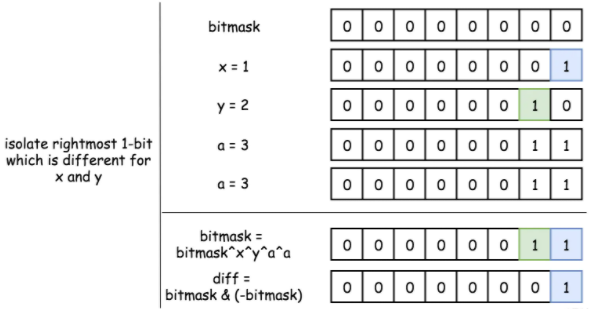
\includegraphics[width=.9\linewidth]{./pic/twoNumberArray.png}

\section{371. Sum of Two Integers}
\label{sec-10-3}
Given two integers a and b, return the sum of the two integers without using the operators + and


一开始自己想的如果两个数都是正数,那么很简单,运用XOR  \^{} 去找出所有的单一的1。接着运用AND \&去找出所有重复的1;重复的1就相当于carryover,需要进位。然后运动<<把重复的1给进位就可以了,最后直接OR一下就等于答案(这是错的,需要每次循环来判断新的进位)。但是发现这个是能运用于两个正数,研究来研究去,不会算带负数的,所以放弃网上找答案。

  发现答案不和我的两个正数之和算法一样嘛!唯一不同的就是答案是把算出的答案继续带回function直到carry等于0;

通过例子来看一下:

a = 5, b = 1:

a: 101

b: 001

根据我最初的算法:(错误的)

sum = a \^{} b = 100

carry = a \& b = 001 这里这个1就是需要进位的

carry = 001 << 1 = 010

最后把sum 100 和 carry 010 OR 一下 就等于 110 = 6。

但是答案的做法却是把sum 和 carry在带回function继续算直至carry = 0, 我们来看一下例子:

a = 5, b = 1:

a = 101

b = 001

sum = 100

carry = 010

带回

a = 100

b = 010

sum = 110

carry = 000 这里等于0了,所以结束,我的理解是,答案的做法是把carryover带回去,和sum比较,如果这一次没有继续需要进位的数字了,就可以结束,否则继续下一轮;换一句话就是,答案是把每一轮的sum和carryover拿出来,下一轮继续加一起看一看有没有新的需要进位的地方,所以明显我之前的做法是错的,我只考虑了一轮而已,实际上是每一轮都有可能有新的需要进位的地方。

那新的问题又来了,为啥负数也可以,这里的负数是2‘s complement:

比如说 -5 = 1111 1111 1111 1111 1111 1111 1111 1011

为何-5 是这样: 首先把上面的bits -1

      1111 1111 1111 1111 1111 1111 1111 1010

然后再flip一下

        0000 0000 0000 0000 0000 0000 0000 0101 = 5. 所以负数都需要先flip一下,然后+1 便成了上面那样。

带负数的两数之和,有点麻烦就是有那么多1,所以利用了自己的想象力来帮助自己理解:(不知道对不对)

举个例子:

a = -5, b = 15

把每一个sum (a) 和 carry (b) 打出来是这样的:
\begin{minted}[frame=lines,fontsize=\scriptsize,linenos=false]{java}
11111111111111111111111111111011
1111
11111111111111111111111111110100
10110
11111111111111111111111111100010
101000
11111111111111111111111111001010
1000000
11111111111111111111111110001010
10000000
11111111111111111111111100001010
100000000
11111111111111111111111000001010
1000000000
11111111111111111111110000001010
10000000000
11111111111111111111100000001010
100000000000
11111111111111111111000000001010
1000000000000
11111111111111111110000000001010
10000000000000
11111111111111111100000000001010
100000000000000
11111111111111111000000000001010
1000000000000000
11111111111111110000000000001010
10000000000000000
11111111111111100000000000001010
100000000000000000
11111111111111000000000000001010
1000000000000000000
11111111111110000000000000001010
10000000000000000000
11111111111100000000000000001010
100000000000000000000
11111111111000000000000000001010
1000000000000000000000
11111111110000000000000000001010
10000000000000000000000
11111111100000000000000000001010
100000000000000000000000
11111111000000000000000000001010
1000000000000000000000000
11111110000000000000000000001010
10000000000000000000000000
11111100000000000000000000001010
100000000000000000000000000
11111000000000000000000000001010
1000000000000000000000000000
11110000000000000000000000001010
10000000000000000000000000000
11100000000000000000000000001010
100000000000000000000000000000
11000000000000000000000000001010
1000000000000000000000000000000
10000000000000000000000000001010
10000000000000000000000000000000
1010
0
10
\end{minted}

我们可以看到最后是10,在我理解,有负数的情况下,我们需要把负数的那些1都过滤一下,所以循环的次数会多很多,相对于正数来说。

通过上面规律,每次a都是减少它的1的数量,每次b都是增多它的0的数量,直到a的1过滤完,b的0达到极限,便结束了,得到正确答案。

利用想象力的时候到了,这就相当于a= -5 b= 15 在一个横坐标上,每一次a向右走一格,b像左走一格,或者说是负数向右走,正数向左走,直到一个最小的负数走到0,那么另外一个数就是答案。

\begin{minted}[frame=lines,fontsize=\scriptsize,linenos=false]{java}
public int getSum(int a, int b) {
    if (b == 0) return a;
    int sum = a ^ b;
    int carry = (a & b) << 1;
    return getSum(sum, carry);
}
public int getSum(int a, int b) { // (-1, 1) 过不了
    if (b == 0) return a;
    int carryOver = 0;
    while (b != 0) { // 这里是 b != 0, b > 0 对负数不成立
        carryOver = (a & b);
        a = a ^ b;
        b = (carryOver << 1);
    }
    return a;
}
\end{minted}

\section{201. Bitwise AND of Numbers Range}
\label{sec-10-4}
Given two integers left and right that represent the range [left, right], return the bitwise AND of all numbers in this range, inclusive.
\begin{minted}[frame=lines,fontsize=\scriptsize,linenos=false]{java}
public int rangeBitwiseAnd(int left, int right) {
    if (left == 0) return 0;
    if (left == 1 && right == Integer.MAX_VALUE) return 0;
    if (Integer.toBinaryString(left).length() != Integer.toBinaryString(right).length()) return 0;
    if (left == right) return left;
    int ans = left;
    for (int i = left+1; i <= right; i++) {
        ans &= i;
        if (ans == 0 || i == Integer.MAX_VALUE) return ans;
    }
    return ans;
}
\end{minted}

\section{1835. Find XOR Sum of All Pairs Bitwise AND - Hard}
\label{sec-10-5}
The XOR sum of a list is the bitwise XOR of all its elements. If the list only contains one element, then its XOR sum will be equal to this element.

For example, the XOR sum of [1,2,3,4] is equal to 1 XOR 2 XOR 3 XOR 4 = 4, and the XOR sum of \footnotemark[1]{} is equal to 3.
You are given two 0-indexed arrays arr1 and arr2 that consist only of non-negative integers.

Consider the list containing the result of arr1[i] AND arr2[j] (bitwise AND) for every (i, j) pair where 0 <= i < arr1.length and 0 <= j < arr2.length.

Return the XOR sum of the aforementioned list.
\begin{minted}[frame=lines,fontsize=\scriptsize,linenos=false]{java}
// Think about (a&b) ^ (a&c). Can you simplify this expression?
// It is equal to a&(b^c).
// Then, (A[i]&B[0])^(A[i]&B[1]).. = A[i]&(B[0]^B[1]^arr[2]...).
// Let bXorSum = (B[0]^B[1]^B[2]...),
// aXorSum = (A[0]^A[1]^A[2]...) so the final answer is
// (bXorSum&A[0]) ^ (bXorSum&A[1]) ^ (bXorSum&A[2]) ^ ... = bXorSum & aXorSum.
public int getXORSum(int[] a, int[] b) {
    int m = a.length;
    int n = b.length;
    int aXorSum = a[0], bXorSum = b[0];
    for (int i = 1; i < m; i++) 
        aXorSum ^= a[i];
    for (int i = 1; i < n; i++) 
        bXorSum ^= b[i];
    return aXorSum & bXorSum;
}
\end{minted}

\section{982. Triples with Bitwise AND Equal To Zero 平生不识 TwoSum,刷尽 LeetCode 也枉然}
\label{sec-10-6}
Given an integer array nums, return the number of AND triples.

An AND triple is a triple of indices (i, j, k) such that:

0 <= i < nums.length
0 <= j < nums.length
0 <= k < nums.length
nums[i] \& nums[j] \& nums[k] == 0, where \& represents the bitwise-AND operator.
\begin{minted}[frame=lines,fontsize=\scriptsize,linenos=false]{java}
//  ‘平生不识 TwoSum,刷尽 LeetCode 也枉然’ 还好不至于哭死呀。。。。。。
public int countTriplets(int[] arr) { 
    Map<Integer, Integer> m = new HashMap<>();
    int v = 0, res = 0;
    for (int i = 0; i < arr.length; i++) 
        for (int j = 0; j < arr.length; j++) {
            v = arr[i] & arr[j];
            m.put(v, m.getOrDefault(v, 0) + 1);
        }
    for (int i = 0; i < arr.length; i++) 
        for (int k : m.keySet()) 
            if ((arr[i] &  k) == 0) res += m.get(k);
    return res;
}
public int countTriplets(int[] arr) { // 这种方法执行起来效率更高一点儿
    int res = 0, v = 0;
    int [] cnt = new int [1 << 16];
    Arrays.fill(cnt, -1);
    for (int a : arr) 
        for (int b : arr) {
            v = a & b;
            if (cnt[v] == -1) {
                cnt[v] = 0;
                for (int c : arr) 
                    if ((v & c) == 0) ++cnt[v];
            }
            res += cnt[v];
        }
    return res;
}
\end{minted}

\section{187. Repeated DNA Sequences - Medium}
\label{sec-10-7}
The DNA sequence is composed of a series of nucleotides abbreviated as 'A', 'C', 'G', and 'T'.

For example, "ACGAATTCCG" is a DNA sequence.
When studying DNA, it is useful to identify repeated sequences within the DNA.

Given a string s that represents a DNA sequence, return all the 10-letter-long sequences (substrings) that occur more than once in a DNA molecule. You may return the answer in any order.

有人说上面native方法超时是因为字符串存储浪费了太多的空间和时间,因此可以考虑用整数存储,即二进制方法。这个思路非常简单,这里一共有四个字母:A,C,G,T。我们转换整数的思路如下:
\begin{minted}[frame=lines,fontsize=\scriptsize,linenos=false]{java}
A = 00,C = 01,G = 10,T = 11。
int key = 0, key = key << 2 | code(A|C|G|T)。
\end{minted}

这样我们就很容易把一个字符串转换为整数了,上面公式不清楚的话,可以直接看转换代码:

\begin{minted}[frame=lines,fontsize=\scriptsize,linenos=false]{java}
private static int hashCode(String s) {
    int hash = 0;
    for (int i = 0; i < s.length(); i++) 
        hash = hash << 2 | mapInteger(s.charAt(i));
    return hash;
}
private static int mapInteger(char c) {
    switch (c) {
    case 'A': return 0;
    case 'C': return 1;
    case 'G': return 2;
    case 'T': return 3;
    default: return 0;
    }
}
public List<String> findRepeatedDnaSequences(String s) {
    List<String> res = new ArrayList<>();
    if (s == null || s.length() == 0) return res;
    Set<Integer> si = new HashSet<>();
    for (int i = 0; i <= s.length()-10; i++) {
        String substr = s.substring(i, i+10);
        Integer key = hashCode(substr);
        if (si.contains(key) && !res.contains(substr))
            res.add(substr);
        else si.add(key);
    }
    return res;
}
\end{minted}
\section{1915. Number of Wonderful Substrings - Medium}
\label{sec-10-8}
A wonderful string is a string where at most one letter appears an odd number of times.

For example, "ccjjc" and "abab" are wonderful, but "ab" is not.
Given a string word that consists of the first ten lowercase English letters ('a' through 'j'), return the number of wonderful non-empty substrings in word. If the same substring appears multiple times in word, then count each occurrence separately.

A substring is a contiguous sequence of characters in a string.
\begin{minted}[frame=lines,fontsize=\scriptsize,linenos=false]{java}
public long wonderfulSubstrings(String word) {
    int n = word.length(), mask = 0, cur = 0;
    long res = 0, cnt = 0;
    Map<Integer, Integer> m = new HashMap<>();
    m.put(0, 1);
    for (int i = 0; i < n; i++) {
        mask ^= (1 << (word.charAt(i)-'a'));
        res += m.getOrDefault(mask, 0);
        m.put(mask, m.getOrDefault(mask, 0) + 1);
        for (int j = 0; j < 10; j++) {
            cur = mask ^ (1 << j);
            res += m.getOrDefault(cur, 0);
        }
    }
    return res;
}
\end{minted}

\section{782. Transform to Chessboard- Hard}
\label{sec-10-9}
You are given an n x n binary grid board. In each move, you can swap any two rows with each other, or any two columns with each other.

Return the minimum number of moves to transform the board into a chessboard board. If the task is impossible, return -1.

A chessboard board is a board where no 0's and no 1's are 4-directionally adjacent.

我们发现对于长度为奇数的棋盘,各行的0和1个数不同,但是还是有规律的,每行的1的个数要么为 n/2,要么为 (n+1)/2,这个规律一定要保证,不然无法形成棋盘。

还有一个很重要的规律,我们观察题目给的第一个例子,如果我们只看行,我们发现只有两种情况 0110 和 1001,如果只看列,只有 0011 和 1100,我们发现不管棋盘有多长,都只有两种情况,而这两种情况上各位上是相反的,只有这样的矩阵才有可能转换为棋盘。那么这个规律可以衍生出一个规律,就是任意一个矩形的四个顶点只有三种情况,要么四个0,要么四个1,要么两个0两个1,不会有其他的情况。那么四个顶点亦或在一起一定是0,所以我们判断只要亦或出了1,一定是不对的,直接返回-1。之后我们来统计首行和首列中的1个数,因为我们要让其满足之前提到的规律。统计完了首行首列1的个数,我们判断如果其小于 n/2 或者大于 (n+1) / 2,那么一定无法转为棋盘。我们还需要算下首行和首列跟棋盘位置的错位的个数,虽然 01010 和 10101 都可以是正确的棋盘,我们先默认跟 10101 比较好了,之后再做优化处理。

最后的难点就是计算最小的交换步数了,这里要分n的奇偶来讨论。如果n是奇数,我们必须得到偶数个,为啥呢,因为我们之前统计的是跟棋盘位置的错位的个数,而每次交换行或者列,会修改两个错位,所以如果是奇数就无法还原为棋盘。举个例子,比如首行是 10001,如果我们跟棋盘 10101 比较,只有一个错位,但是我们是无法通过交换得到 10101的,所以我们必须要交换得到 01010,此时的错位是4个,而我们通过 n - rowDiff 正好也能得到4,这就是为啥我们需要偶数个错位。如果n是偶数,那么就不会出现这种问题,但是会出现另一个问题,比如我们是 0101,这本身就是正确的棋盘排列了,但是由于我们默认是跟 1010 比较,那么我们会得到4个错位,所以我们应该跟 n - rowDiff 比较取较小值。列的处理跟行的处理完全一样。最终我们把行错位个数跟列错位个数相加,再除以2,就可以得到最小的交换次数了,之前说过了每交换一次,可以修复两个错位,参见代码如下:

\begin{minted}[frame=lines,fontsize=\scriptsize,linenos=false]{java}
public int movesToChessboard(int[][] bd) { // bd: board
    int n = bd.length, rowSum = 0, colSum = 0, rowDif = 0, colDif = 0;
    for (int i = 0; i < n; i++) 
        for (int j = 0; j < n; j++)
            if ((bd[0][0] ^ bd[i][0] ^ bd[0][j] ^ bd[i][j]) > 0) return -1;
    for (int i = 0; i < n; i++) {
        rowSum += bd[0][i];
        colSum += bd[i][0];
        rowDif += bd[i][0] == i % 2 ? 1 : 0; // 
        colDif += bd[0][i] == i % 2 ? 1 : 0; // 
    }
    if (rowSum < n/2 || rowSum > (n+1)/2) return -1;
    if (colSum < n/2 || colSum > (n+1)/2) return -1;
    if (n % 2 == 1) {
        if (rowDif % 2 == 1) rowDif = n - rowDif;
        if (colDif % 2 == 1) colDif = n - colDif;
    } else {
        rowDif = Math.min(rowDif, n - rowDif);
        colDif = Math.min(colDif, n - colDif);
    }
    return (rowDif + colDif) / 2;
}
\end{minted}
\begin{itemize}
\item 方法一:分维度计算【通过】
\end{itemize}
思路

首先需要思考的是一次交换之后,棋盘会发生什么变化。为了简单起见,这里用交换列来做例子。在对任意两列进行交换之后,可以看到列交换是不会改变任意两行之间的状态的,简单的来说如果这两行原本就相同,列交换之后这两行依旧相同,如果这两行本来就不同,列交换之后也还是不同。由于最终的棋盘只有两种不同的行,最初的棋盘也一定只有两种不同的行,否则不管怎么做列交换都不会得到最终的棋盘。

之后再来看棋盘行的规律,棋盘有两种行,这两种行每一位都互相不同。同时对于每一行来说,一定有一半为 1,一半为 0(如果长度为奇数,会多一个 1 或多一个 0)。对于棋盘的列也是同样的规律。

可以观察到,先换行再换列跟先换列再换行结果是一样的。在这里先将所有的行调到正确的位置,再将所有的列调到正确的位置。

考虑到只有两种不同的行,可以分别用 0,1 对其表示。要达成最终的棋盘实际上等价于将棋盘的行表示成 0,1相隔的状态。假设在将棋盘的行用 0,1 表示之后得到数组为 [0, 1, 1, 1, 0, 0],那么只需求这个数组变成 [0, 1, 0, 1, 0, 1] 和 [1, 0, 1, 0, 1, 0] 的代价,之后取其中最小的代价就好了。同理,对列也是如此,这就将二维问题变成了两个一维问题。

算法

首先需要确认是否有且只有两种行(列)存在,且这两种行(列)的 0,1 排布合法,如果不符合条件直接返回 -1。之后需要生成理想的行(列)的状态(即0,1相隔的数组排列),对于每种理想状态,计算其与初始状态之间变换的代价。举个例子,对于 [0, 1, 1, 1, 0, 0] 初始状态来说,有两种理想状态,分别是 [0, 1, 0, 1, 0, 1] 和 [1, 0, 1, 0, 1, 0],对于 [0, 1, 1, 1, 0] 初始状态只有一种理想状态 [1, 0, 1, 0, 1]。

在 Java 实现中,用整型来表示每行。之后将其与 0b010101010101\ldots{}..01 进行异或来计算初始状态转换到理想状态的代价。为了代码简洁,这里统一使用 0xAAAAAAAA 和 0x55555555,为了不引入额外的转换代价,还需要根据行的长度 N 生成 0b00\ldots{}0011\ldots{}11 掩码与结果做与运算。
\begin{minted}[frame=lines,fontsize=\scriptsize,linenos=false]{java}
public int movesToChessboard(int[][] board) {
    int N = board.length;
    // count[code] = v, where code is an integer
    // that represents the row in binary, and v
    // is the number of occurrences of that row
    Map<Integer, Integer> count = new HashMap();
    for (int[] row: board) {
        int code = 0;
        for (int x: row)
            code = 2 * code + x;
        count.put(code, count.getOrDefault(code, 0) + 1);
    }
    int k1 = analyzeCount(count, N);
    if (k1 == -1) return -1;
    // count[code], as before except with columns
    count = new HashMap();
    for (int c = 0; c < N; ++c) {
        int code = 0;
        for (int r = 0; r < N; ++r)
            code = 2 * code + board[r][c];
        count.put(code, count.getOrDefault(code, 0) + 1);
    }
    int k2 = analyzeCount(count, N);
    return k2 >= 0 ? k1 + k2 : -1;
}
public int analyzeCount(Map<Integer, Integer> count, int N) {
    // Return -1 if count is invalid
    // Otherwise, return number of swaps required
    if (count.size() != 2) return -1;
    List<Integer> keys = new ArrayList(count.keySet());
    int k1 = keys.get(0), k2 = keys.get(1);
    // If lines aren't in the right quantity
    if (!(count.get(k1) == N/2 && count.get(k2) == (N+1)/2) &&
        !(count.get(k2) == N/2 && count.get(k1) == (N+1)/2))
        return -1;
    // If lines aren't opposite
    if ((k1 ^ k2) != (1<<N) - 1)
        return -1;
    int Nones = (1 << N) - 1;
    int ones = Integer.bitCount(k1 & Nones); // bitCount统计二进制中1的个数
    int cand = Integer.MAX_VALUE;
    if (N%2 == 0 || ones * 2 < N) // zero start
        cand = Math.min(cand, Integer.bitCount(k1 ^ 0xAAAAAAAA & Nones) / 2);
    if (N%2 == 0 || ones * 2 > N) // ones start
        cand = Math.min(cand, Integer.bitCount(k1 ^ 0x55555555 & Nones) / 2);
    return cand;
}
\end{minted}

\section{1803. Count Pairs With XOR in a Range - Hard}
\label{sec-10-10}
Given a (0-indexed) integer array nums and two integers low and high, return the number of nice pairs.

A nice pair is a pair (i, j) where 0 <= i < j < nums.length and low <= (nums[i] XOR nums[j]) <= high.
\begin{itemize}
\item 1. 暴力算法
\end{itemize}

直接暴力计算,利用 num$^{\text{num2}}$=i 等效于 num$^{\text{i}}$=num2 的特点,先统计当前各个数字出现的次数,再将当前数字和 [low, high] 范围内的数字进行异或运算,将其结果对应的出现次数相加。

\begin{minted}[frame=lines,fontsize=\scriptsize,linenos=false]{java}
public int countPairs(int[] arr, int low, int high) { 
    int [] freq = new int [20002]; // nums[i]<=20000
    for (int v : arr)
        freq[v]++;
    int val = 0, res = 0;
    for (int v : arr) {
        for (int i = low; i <= high; i++) {
            val = v ^ i;     // num ^ i = num2 <==> num ^ num2 = i
            if (val <= 20000)
                res += freq[val]; // v^val=i中当前v对应val出现的次数
        }
        freq[v]--;           // 当前v所有组合已统计,减去出现次数,避免重复
    }
    return res;
}
\end{minted}
\begin{itemize}
\item 2. 字典树(Trie树)
\end{itemize}
(1)思路
在上述算法的基础上,结合字典树方法快速统计。在依次将 nums 中数字加入字典树的同时,搜索和该数字异或值在 [0, high] 和 [0, low - 1] 范围内数字 num2 的个数并相减,就是符合异或值为 [low, high] 区间内的数字个数。
\begin{minted}[frame=lines,fontsize=\scriptsize,linenos=false]{java}
public class Trie {
    static final int H = 14; // 2^15=32768,15位二进制足够计算
    int cnt;
    Trie [] next;
    public Trie() {
        this.cnt = 0;
        this.next = new Trie[2];
    }
    public void insert(int va) { // 插入数值
        Trie r = this;
        for (int i = H; i >= 0; i--) {
            int bit = (va >> i) & 1;
            if (r.next[bit] == null)
                r.next[bit] = new Trie();
            r = r.next[bit];
            r.cnt++;
        }
    } 
    public int search(Trie r, int digit, int v, int range) { // 搜索和 v 异或值在[0,range]范围内的数字num2的个数
        if (r == null) return 0;
        if (digit < 0) return r.cnt;
        int vb = (v >> digit) & 1;    // v 和 range 在该位的值
        int vr = (range >> digit) & 1;
        if (vr == 1) {   // range在该位为1
            if (vb == 0) // num 在该位为0,num2该位为0的部分全部满足,为1的部分继续判断
                return (r.next[0] == null ? search(r.next[1], digit-1, v, range) : r.next[0].cnt + search(r.next[1], digit-1, v, range));
            else         // v 在该位为1,num2该位为1的部分全部满足,为0的部分继续判断
                return (r.next[1] == null ? search(r.next[0], digit-1, v, range) : r.next[1].cnt + search(r.next[0], digit-1, v, range));
        }
        return search(r.next[vb], digit-1, v, range); // range在该位 vr 为0,num2该位必须和num一致
    }
}
private Trie root;
public int countPairs(int[] arr, int low, int high) {
    int n = arr.length, maxHeight = 14; // 2^15=32768,15位二进制足够计算
    int res = 0;
    root = new Trie();
    for (int v : arr) {
        res += root.search(root, maxHeight, v, high) - root.search(root, maxHeight, v, low-1); // 这里的脑袋好难转呀。。。
        root.insert(v);
    }
    return res;
    // for (int v : arr) 
    //     root.insert(v);
    // for (int v : arr) 
    //     res += root.search(root, maxHeight, v, high) - root.search(root, maxHeight, v, low-1);
    // return res / 2; // 如果按这种写法,就得 / 2,智商呢?!!!
}
\end{minted}

\section{1734. Decode XORed Permutation - Medium}
\label{sec-10-11}
There is an integer array perm that is a permutation of the first n positive integers, where n is always odd.

It was encoded into another integer array encoded of length n - 1, such that encoded[i] = perm[i] XOR perm[i + 1]. For example, if perm = [1,3,2], then encoded = [2,1].

Given the encoded array, return the original array perm. It is guaranteed that the answer exists and is unique.

结合 n 为奇数的特点,先对 encoded 数组中下标为奇数的元素进行异或,得到第 2 到 n 个数的异或值;

因为整数数组是前 n 个正整数的排列,再对 1 到 n 进行异或,得到全部数的异或值;

上述二者进行异或即可得到第 1 个数,然后依次求解获得其他数字,得到原始数组。
\begin{minted}[frame=lines,fontsize=\scriptsize,linenos=false]{java}
public int[] decode(int[] encoded) {
    int n = encoded.length + 1;
    int xor = 0, vFrom2 = 0;
    for (int i = 1; i < n-1; i += 2)  // 记录第2到n个数的异或值
        vFrom2 = vFrom2 ^ encoded[i]; // (a[1]^a[2])^(a[3]^a[4])^...^(a[n-2]^a[n-1])
    for (int i = 1; i <= n; i++)      // a[0]^a[1]^a[2]^...^a[n-1]
        xor ^= i;
    int [] arr = new int [n];
    arr[0] = xor ^ vFrom2;
    for (int i = 1; i < n; i ++)
        arr[i] = arr[i-1] ^ encoded[i-1];
    return ans;
}
\end{minted}

\section{957. Prison Cells After N Days - Medium}
\label{sec-10-12}
There are 8 prison cells in a row and each cell is either occupied or vacant.

Each day, whether the cell is occupied or vacant changes according to the following rules:

If a cell has two adjacent neighbors that are both occupied or both vacant, then the cell becomes occupied.
Otherwise, it becomes vacant.
Note that because the prison is a row, the first and the last cells in the row can't have two adjacent neighbors.

You are given an integer array cells where cells[i] \texttt{= 1 if the ith cell is occupied and cells[i] =} 0 if the ith cell is vacant, and you are given an integer n.

Return the state of the prison after n days (i.e., n such changes described above).
\begin{minted}[frame=lines,fontsize=\scriptsize,linenos=false]{java}
Input: cells = [0,1,0,1,1,0,0,1], N = 7
Output: [0,0,1,1,0,0,0,0]
Explanation: The following table summarizes the state of the prison on each day:
Day 0: [0, 1, 0, 1, 1, 0, 0, 1]
Day 1: [0, 1, 1, 0, 0, 0, 0, 0]
Day 2: [0, 0, 0, 0, 1, 1, 1, 0]
Day 3: [0, 1, 1, 0, 0, 1, 0, 0]
Day 4: [0, 0, 0, 0, 0, 1, 0, 0]
Day 5: [0, 1, 1, 1, 0, 1, 0, 0]
Day 6: [0, 0, 1, 0, 1, 1, 0, 0]
Day 7: [0, 0, 1, 1, 0, 0, 0, 0]
\end{minted}
博主最开始做的时候,看题目标记的是 Medium,心想应该不需要啥特别的技巧,于是就写了一个暴力破解的,但是超时了 Time Limit Exceeded。给了一个超级大的N,不得不让博主怀疑是否能够直接遍历N,又看到了本题的标签是 Hash Table,说明了数组的状态可能是会有重复的,就是说可能是有一个周期循环的,这样就完全没有必要每次都算一遍。正确的做法的应该是建立状态和当前N值的映射,一旦当前计算出的状态在 HashMap 中出现了,说明周期找到了,这样就可以通过取余来快速的缩小N值。为了使用 HashMap 而不是 TreeMap,这里首先将数组变为字符串,然后开始循环N,将当前状态映射为 N-1,然后新建了一个长度为8,且都是0的字符串。更新的时候不用考虑首尾两个位置,因为前面说了,首尾两个位置一定会变为0。更新完成了后,便在 HashMap 查找这个状态是否出现过,是的话算出周期,然后N对周期取余。最后再把状态字符串转为数组即可,参见代码如下:
\begin{minted}[frame=lines,fontsize=\scriptsize,linenos=false]{cpp}
vector<int> prisonAfterNDays(vector<int>& cells, int N) {
    vector<int> res;
    string str;
    for (int num : cells) str += to_string(num);
    unordered_map<string, int> m;
    while (N > 0) {
        m[str] = N--;
        string cur(8, '0');
        for (int i = 1; i < 7; ++i) {
            cur[i] = (str[i - 1] == str[i + 1]) ? '1' : '0';
        }
        str = cur;
        if (m.count(str)) {
            N %= m[str] - N;
        }
    }
    for (char c : str) res.push_back(c - '0');
    return res;
}
\end{minted}
下面的解法使用了 TreeMap 来建立状态数组和当前N值的映射,这样就不用转为字符串了,写法是简单了一点,但是运行速度下降了许多,不过还是在 OJ 许可的范围之内,参见代码如下:
\begin{minted}[frame=lines,fontsize=\scriptsize,linenos=false]{cpp}
vector<int> prisonAfterNDays(vector<int>& cells, int N) {
    map<vector<int>, int> m;
    while (N > 0) {
        m[cells] = N--;
        vector<int> cur(8);
        for (int i = 1; i < 7; ++i) {
            cur[i] = (cells[i - 1] == cells[i + 1]) ? 1 : 0;
        }
        cells = cur;
        if (m.count(cells)) {
            N %= m[cells] - N;
        }
    }
    return cells;
}
\end{minted}
\begin{itemize}
\item 下面这种解法是看 lee215 大神的帖子 中说的这个循环周期是 1,7,或者 14,知道了这个规律后,直接可以在开头就对N进行缩小处理,取最大的周期 14,使用 (N-1) \% 14 + 1 的方法进行缩小,至于为啥不能直接对 14 取余,是因为首尾可能会初始化为1,而一旦N大于0的时候,返回的状态首尾一定是0。为了不使得正好是 14 的倍数的N直接缩小为0,所以使用了这么个小技巧,参见代码如下:
\end{itemize}
\begin{minted}[frame=lines,fontsize=\scriptsize,linenos=false]{cpp}
vector<int> prisonAfterNDays(vector<int>& cells, int N) {
    for (N = (N - 1) % 14 + 1; N > 0; --N) {
        vector<int> cur(8);
        for (int i = 1; i < 7; ++i) {
            cur[i] = (cells[i - 1] == cells[i + 1]) ? 1 : 0;
        }
        cells = cur;
    }
    return cells;
}
\end{minted}
\begin{minted}[frame=lines,fontsize=\scriptsize,linenos=false]{java}
public int[] prisonAfterNDays(int[] arr, int n) {
    int m = 8, cnt = 0;
    int [] tmp = arr.clone();
    while (cnt < (n % 14 == 0 ? 14 : n % 14)) { 
        Arrays.fill(tmp, 0);
        for (int i = 1; i < m-1; i++) 
            tmp[i] = 1- (arr[i-1] ^ arr[i+1]);
        arr = tmp.clone();
        ++cnt;
    }
    return arr;
}
\end{minted}
\begin{itemize}
\item 还有一个大神级的思路
\end{itemize}
since N might be pretty large, so we can’t starting from times 1 to times N, No matter what the rules are, the states might be reappear after a certain times of proceeding(because we have fixed number of different states.)

but for different initial state, it might take different steps to reach back to this same state.

so we need to calculate the length of that. and based on N, we can get what we want after N steps.

This is the method called fast-forward.

and if the number of possible states is very large, say 10$^{\text{10}}$, and it’s even larger than N, then calculate the length of repetitive pattern is not acceptable.
but in this problem, there will be 2$^{\text{8}}$ number of possible states. so we can calculate the length of cycle.

however, think twice about it. each time we need to check if this is a repetitive pattern of initial state. this is time consuming.

Solution2:

we have a better solution, in stead of change each digit at a time for each transaction, we use bit map, based on the follow rule:

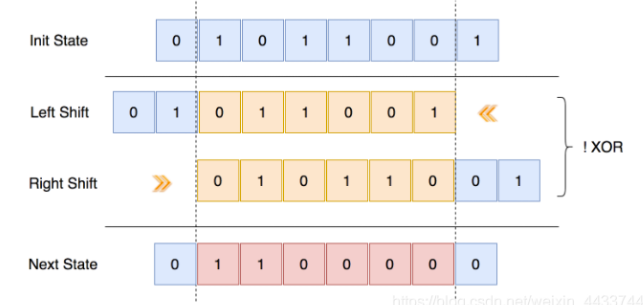
\includegraphics[width=.9\linewidth]{./pic/prisonCell.png}

\begin{minted}[frame=lines,fontsize=\scriptsize,linenos=false]{java}
public int[] prisonAfterNDays(int[] cells, int N) {
    HashMap<Integer, Integer> seen = new HashMap<>();
    boolean isFastForwarded = false;
    // step 1). convert the cells to bitmap
    int stateBitmap = 0x0;
    for (int cell : cells) {
        stateBitmap <<= 1;
        stateBitmap = (stateBitmap | cell);
    }
    // step 2). run the simulation with hashmap
    while (N > 0) {
        if (!isFastForwarded) {
            if (seen.containsKey(stateBitmap)) {
                // the length of the cycle is seen[state_key] - N
                N %= seen.get(stateBitmap) - N;
                isFastForwarded = true;
            } else
                seen.put(stateBitmap, N);
        }
        // check if there is still some steps remained,
        // with or without the fast forwarding.
        if (N > 0) {
            N -= 1;
            stateBitmap = this.nextDay(stateBitmap);
        }
    }
    // step 3). convert the bitmap back to the state cells
    int ret[] = new int[cells.length];
    for (int i = cells.length - 1; i >= 0; i--) {
        ret[i] = (stateBitmap & 0x1);
        stateBitmap = stateBitmap >> 1;
    }
    return ret;
}
protected int nextDay(int stateBitmap) {
    stateBitmap = ~(stateBitmap << 1) ^ (stateBitmap >> 1);
    // set the head and tail to zero
    stateBitmap = stateBitmap & 0x7e;
    return stateBitmap;
}
\end{minted}

\chapter{Bit Masks}
\label{sec-11}
\section{总结一下}
\label{sec-11-1}
对于一个含有 N 个元素的集合,其总共包含  个子集,因此有  个掩码的可能,每一个掩码表示一个子集。事实上,每一个掩码就是一个用二进制表示的整数,比如 1001 就是 9 。

Bitmasking 是为每个掩码分配一个值(即为每个子集分配一个值),然后使用已经计算出的掩码值来计算新掩码的值。通常,我们的主要目标是为整个集合(即掩码11111111)计算值。

要计算子集 X 的值,我们要么以各种可能的方式删除元素,并将获得的子集的值, 来计算 X 的值或解。这意味着  的值必须已经计算过,因此我们需要考虑掩码计算的先后顺序。

最容易想到就是自然序:按相应数字的递增顺序遍历并计算掩码所对应的解。同样,我们一般从空的子集 X 开始,然后以各种可能的方式添加元素,并使用解已知的子集 的值来计算 X 的值/解。

掩码常见的操作和表示:bit(i,mask) 表示取掩码的第 i 位count(mask)  表示掩码中非零位的个数first(mask)  表示掩码中最低非零位的数目set(i,mask) 表示设置掩码中的第 i 位check(i,mask) 表示检查掩码中的第 i 位

而在基于状态压缩的动态规划中,我们常用到以下四种计算操作:

\begin{itemize}
\item 若当前状态为 S,对 S 有下列操作。
\begin{itemize}
\item ①判断第 i 位是否为0: (S \& (1 << i))== 0,意思是将 1 左移 i 位与 S 进行与运算后,看结果是否为零。
\item ②将第 i 位设置为1:S|(1 << i),意思是将 1 左移 i 位与 S 进行或运算。
\item ③将第 i 位设置为0:S \& \textasciitilde{}(1 << i) ,意思是将 S 与第 i 位为 0,其余位为 1 的数进行与运算;
\item ④取第 i 位的值:S \& (1 << i)
\end{itemize}
\end{itemize}

\section{1659. Maximize Grid Happiness - Hard}
\label{sec-11-2}
You are given four integers, m, n, introvertsCount, and extrovertsCount. You have an m x n grid, and there are two types of people: introverts and extroverts. There are introvertsCount introverts and extrovertsCount extroverts.

You should decide how many people you want to live in the grid and assign each of them one grid cell. Note that you do not have to have all the people living in the grid.

The happiness of each person is calculated as follows:

Introverts start with 120 happiness and lose 30 happiness for each neighbor (introvert or extrovert).
Extroverts start with 40 happiness and gain 20 happiness for each neighbor (introvert or extrovert).
Neighbors live in the directly adjacent cells north, east, south, and west of a person's cell.

The grid happiness is the sum of each person's happiness. Return the maximum possible grid happiness.

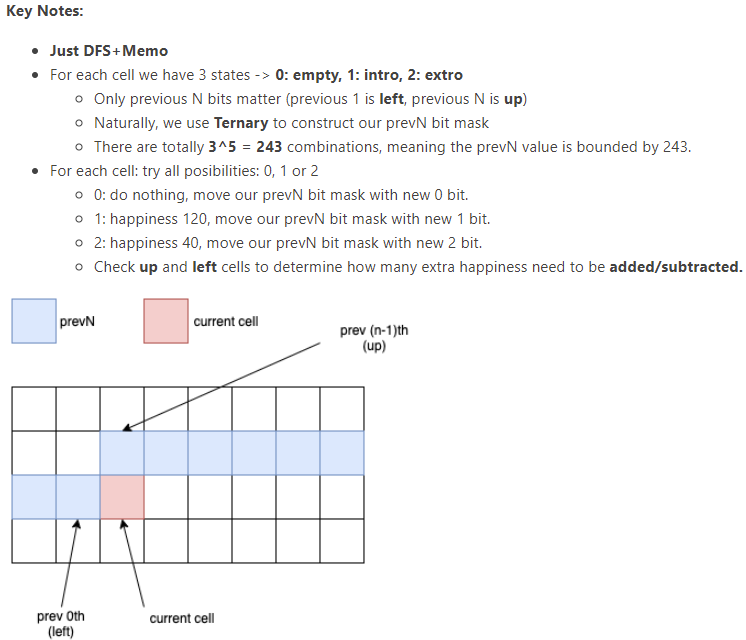
\includegraphics[width=.9\linewidth]{./pic/happiness.png} 
\begin{minted}[frame=lines,fontsize=\scriptsize,linenos=false]{java}
public int getMaxGridHappiness(int m, int n, int introvertsCount, int extrovertsCount) {
    return helper(m, n, 0, 0, introvertsCount, extrovertsCount, 0, new Integer[m][n][introvertsCount+1][extrovertsCount+1][243]);
}        
private int get(int preN, int i) {       // Ternary get ith bit value (0, 1 or 2)
    preN /= ((int) Math.pow(3, i));
    return preN % 3;
}
private int set(int curRow, int value) { // Ternary set new-coming bit to value
    return (curRow * 3 + value) % 243;
}                                        // Ternary bit meaning -> empty: 0, intro: 1, extro: 2
private int helper(int m, int n, int x, int y, int inCnt, int exCnt, int preN, Integer [][][][][] dp) {
    if (y == n) { // advance pointer
        y = 0;
        x++;
    }
    if (inCnt == 0 && exCnt == 0) return 0;
    if (x == m) return 0;
    if (dp[x][y][inCnt][exCnt][preN] != null) return dp[x][y][inCnt][exCnt][preN];
    int res = helper(m, n, x, y+1, inCnt, exCnt, set(preN, 0), dp); // leave the cell empty
    int up = get(preN, n-1); // get up bit -> which is at (n - 1)th
    int left = get(preN, 0); // get left bit -> which is at (0)th
    if (inCnt > 0) {
        int cur = preN;
        cur = set(cur, 1); // set new-coming bit to 1
        int addOn = 120;
        if (x-1 >= 0 && up != 0) { // up: 1 or 2
            addOn -= 30;
            if (up == 1) addOn -= 30;
            else addOn += 20;
        }
        if (y-1 >= 0 && left != 0) {
            addOn -= 30;
            if (left == 1) addOn -= 30;
            else addOn += 20;
        }
        res = Math.max(res, helper(m, n, x, y+1, inCnt-1, exCnt, cur, dp) + addOn);
    }
    if (exCnt > 0) {
        int cur = preN;
        cur = set(cur, 2); // set new-coming bit to 1
        int addOn = 40 ;
        if (x-1 >= 0 && up != 0) { // up: 1 or 2
            addOn += 20;
            if (up == 1) addOn -= 30;
            else addOn += 20;
        }
        if (y-1 >= 0 && left != 0) {
            addOn += 20;
            if (left == 1) addOn -= 30;
            else addOn += 20;
        }
        res = Math.max(res, helper(m, n, x, y+1, inCnt  , exCnt-1, cur, dp) + addOn);
    }
    return dp[x][y][inCnt][exCnt][preN] = res;
}
\end{minted}

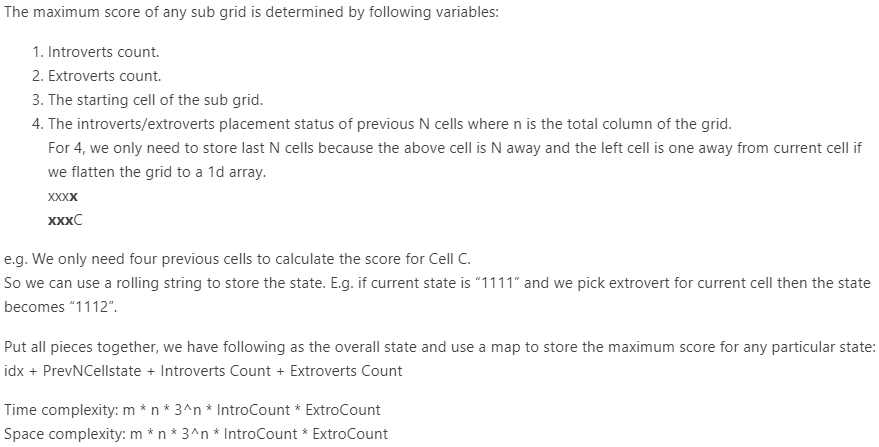
\includegraphics[width=.9\linewidth]{./pic/happiness2.png} 
\begin{minted}[frame=lines,fontsize=\scriptsize,linenos=false]{java}
public int getMaxGridHappiness(int m, int n, int introvertsCount, int extrovertsCount) {
    Map<String, Integer> memo = new HashMap<>();
    return helper("0".repeat(n), 0, m, n, introvertsCount, extrovertsCount, memo);
}
private int helper(String state, int idx, int m, int n, int inCnt, int exCnt, Map<String, Integer> memo) {
    if (inCnt == 0 && exCnt == 0 || idx == m*n) return 0;
    String key = idx + state + inCnt + exCnt;
    if (memo.containsKey(key)) return memo.get(key);
    int i = idx / n, j = idx % n;
    int max = 0;
    if (inCnt > 0) { // case 1: place an introvert in this cell if possible.
        int curVal = 120;
        if (i > 0) curVal = calScore(state.charAt(0)-'0', 1, curVal);
        if (j > 0) curVal = calScore(state.charAt(state.length()-1)-'0', 1, curVal);
        max = Math.max(max, helper(state.substring(1)+"1", idx+1, m, n, inCnt-1, exCnt, memo) + curVal);
    }
    if (exCnt > 0) { // case 2: place an extrovert in this cell if possible.
        int curVal = 40;
        if (i > 0) curVal = calScore(state.charAt(0)-'0', 2, curVal);
        if (j > 0) curVal = calScore(state.charAt(state.length()-1)-'0', 2, curVal);
        max = Math.max(max, helper(state.substring(1)+"2", idx+1, m, n, inCnt, exCnt-1, memo) + curVal);
    }                // case 3: Do not place any person.
    max = Math.max(max, helper(state.substring(1)+"0", idx+1, m, n, inCnt, exCnt, memo)); // 不要忘记这种选择
    memo.put(key, max);
    return max;
}
private int calScore(int i, int j, int v) {
    if (i == 1 && j == 1) return v - 60;
    if (i == 2 && j == 2) return v + 40;
    if (i == 1 && j == 2 || i == 2 && j == 1) return v - 10;
    return v;
}
\end{minted}
\begin{itemize}
\item 还有一种其它语言写的,行与行之间以行为单位进行动态规划状态转移的,可以搜出来参考一下
\end{itemize}
\section{1494. Parallel Courses II - Hard}
\label{sec-11-3}
You are given an integer n, which indicates that there are n courses labeled from 1 to n. You are also given an array relations where relations[i] = [prevCoursei, nextCoursei], representing a prerequisite relationship between course prevCoursei and course nextCoursei: course prevCoursei has to be taken before course nextCoursei. Also, you are given the integer k.

In one semester, you can take at most k courses as long as you have taken all the prerequisites in the previous semester for the courses you are taking.

Return the minimum number of semesters needed to take all courses. The testcases will be generated such that it is possible to take every course.
\begin{minted}[frame=lines,fontsize=\scriptsize,linenos=false]{java}
public int minNumberOfSemesters(int n, int [][] relations, int k) {
    int [] pre = new int [n]; // bitmask representing prerequirements
    for (int i = 0; i < relations.length; i++) {
        int u = relations[i][0] - 1;
        int v = relations[i][1] - 1;
        pre[v] |= (1 << u);
    }
    int range = (1 << n);
    int [] cnt = new int [range]; // 所有的状态只数一遍位数
    for (int i = 0; i < range; i++) 
        cnt[i] = Integer.bitCount(i);
    int [] dp = new int [range];  // dp[state] = minimum semesters to complete all the courses of 'state'.
    Arrays.fill(dp, n);
    dp[0] = 0;
    for (int i = 0; i < range; i++) {
        int available = 0;
        for (int j = 0; j < n; j++) 
            if ((i & pre[j]) == pre[j]) // 可是包含了忆经选过的课程
                available |= (1 << j);  // Can study course j next, since all required courses have been studied.
        available &= ~i; // Don't want to study those already studied courses.
        int nextCourses = available;
        while (nextCourses > 0) {
            if (cnt[nextCourses] <= k)
                dp[i | nextCourses] = Math.min(dp[i | nextCourses], dp[i] + 1);
// 遍历现在可选课程的所有子集:Enumerate all subsets. E.g, available = 101, next: 100 -> 001 -> 000
            nextCourses = (nextCourses -1) & available; 
        }
    }
     return dp[range-1];
}
\end{minted}
\begin{itemize}
\item 另一种用以++写的递归的
\end{itemize}

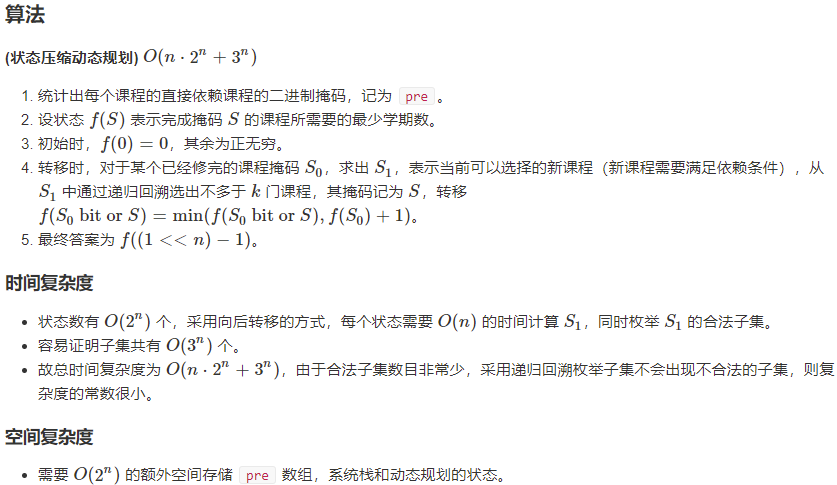
\includegraphics[width=.9\linewidth]{./pic/courseII.png}
\begin{minted}[frame=lines,fontsize=\scriptsize,linenos=false]{cpp}
void solve(int i, int s, int k, int n, int s0, int s1, vector<int> &f) {
    if (k == 0 || i == n) {
        f[s0 | s] = min(f[s0 | s], f[s0] + 1);
        return;
    }
    solve(i + 1, s, k, n, s0, s1, f);
    if ((s1 >> i) & 1)
        solve(i + 1, s | 1 << i, k - 1, n, s0, s1, f);
}
int minNumberOfSemesters(int n, vector<vector<int>>& dependencies, int k) {
    vector<int> pre(n, 0);
    for (const auto &v : dependencies)
        pre[v[1] - 1] |= 1 << (v[0] - 1);
    vector<int> f(1 << n, INT_MAX);
    f[0] = 0;
    for (int s0 = 0; s0 < (1 << n); s0++) {
        if (f[s0] == INT_MAX)
            continue;
        int s1 = 0;
        for (int i = 0; i < n; i++)
            if (!((s0 >> i) & 1) && ((pre[i] & s0) == pre[i]))
                s1 |= 1 << i;
        solve(0, 0, k, n, s0, s1, f);
    }
    return f[(1 << n) - 1];
}
\end{minted}

\section{1815. Maximum Number of Groups Getting Fresh Donuts - Hard}
\label{sec-11-4}
There is a donuts shop that bakes donuts in batches of batchSize. They have a rule where they must serve all of the donuts of a batch before serving any donuts of the next batch. You are given an integer batchSize and an integer array groups, where groups[i] denotes that there is a group of groups[i] customers that will visit the shop. Each customer will get exactly one donut.

When a group visits the shop, all customers of the group must be served before serving any of the following groups. A group will be happy if they all get fresh donuts. That is, the first customer of the group does not receive a donut that was left over from the previous group.

You can freely rearrange the ordering of the groups. Return the maximum possible number of happy groups after rearranging the groups.

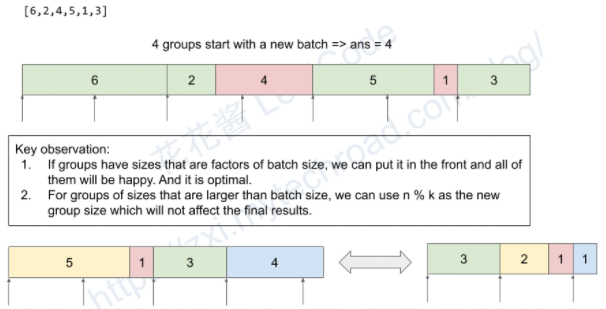
\includegraphics[width=.9\linewidth]{./pic/donut.png}

\begin{minted}[frame=lines,fontsize=\scriptsize,linenos=false]{java}
private int dfsBackTracking(int [] cnt, int batchSize, int lastGroup, int leftOverGroups) { // DFS+记忆化搜索求最多开心组数
    if (leftOverGroups == 0) return 0;
    String key = Arrays.toString(cnt); // 剩余组情况生成String作为哈希表的键, this is so called HASHING
    if (dp.containsKey(key)) return dp.get(key);
    int res = 0;
    for (int i = 1; i < batchSize; i++) {
        if (cnt[i] == 0) continue;
        --cnt[i]; 
        res = Math.max(res, dfsBackTracking(cnt, batchSize, lastGroup+i, leftOverGroups-1) + (lastGroup % batchSize == 0 ? 1 : 0));
        ++cnt[i]; 
    }
    dp.put(key, res);
    return res;
}
Map<String, Integer> dp;
int n;
public int maxHappyGroups(int batchSize, int[] groups) { // group size 30 is too large for backtracking WITHOUT modifications
    n = groups.length;
    int [] cnt = new int [batchSize];
    for (int v : groups) 
        cnt[v % batchSize]++;
    dp = new HashMap<>();
    return dfsBackTracking(cnt, batchSize, 0, n-cnt[0]) + cnt[0];
}
\end{minted}
\begin{itemize}
\item 一点儿稍微的优化,以减少回溯backtracking的耗时
\end{itemize}
\begin{minted}[frame=lines,fontsize=\scriptsize,linenos=false]{java}
private int dfsBackTracking(int [] cnt, int batchSize, int lastGroup, int leftOverGroups) { // DFS+记忆化搜索求最多开心组数
    if (leftOverGroups == 0) return 0;
    String key = Arrays.toString(cnt); // 剩余组情况生成String作为哈希表的键, this is so called HASHING
    if (dp.containsKey(key)) return dp.get(key);
    int res = 0;
    for (int i = 1; i < batchSize; i++) {
        if (cnt[i] == 0) continue;
        --cnt[i]; 
        res = Math.max(res, dfsBackTracking(cnt, batchSize, lastGroup+i, leftOverGroups-1) + (lastGroup % batchSize == 0 ? 1 : 0));
        ++cnt[i]; 
    }
    dp.put(key, res);
    return res;
}
Map<String, Integer> dp;
int n;
public int maxHappyGroups(int batchSize, int[] groups) { // group size 30 is too large for backtracking WITHOUT modifications
    n = groups.length;
    int [] cnt = new int [batchSize];
    for (int v : groups) 
        cnt[v % batchSize]++;
    // take out the 2 remainder's min groups if their sum is batchSize.
    // it still works but slow without this step
    // Note: < batchSize / 2 to avoid when i is batchSize / 2 it will subtract itself
    int res = cnt[0], min = 0;
    for (int i = 1; i < batchSize/2; i++) {
        min = Math.min(cnt[i], cnt[batchSize-i]);
        cnt[i] -= min;
        cnt[batchSize-i] -= min;
        res += min;
    }
    dp = new HashMap<>();
    return res + dfsBackTracking(cnt, batchSize, 0, n-cnt[0]);
}
\end{minted}
\begin{itemize}
\item 压缩方法里的参数
\end{itemize}
\begin{minted}[frame=lines,fontsize=\scriptsize,linenos=false]{java}
private int dfsBackTracking(int [] cnt, int batchSize, int s) { // DFS+记忆化搜索
    String key = Arrays.toString(cnt); 
    if (dp.containsKey(key)) return dp.get(key);
    int res = 0;
    for (int i = 1; i < batchSize; i++) {
        if (cnt[i] == 0) continue;
        --cnt[i]; 
        res = Math.max(res, dfsBackTracking(cnt, batchSize, (s+i) % batchSize) + (s == 0 ? 1 : 0));
        ++cnt[i]; 
    }
    dp.put(key, res);
    return res;
}
Map<String, Integer> dp;
int n;
public int maxHappyGroups(int batchSize, int[] groups) { 
    n = groups.length;
    int [] cnt = new int [batchSize];
    for (int v : groups) 
        cnt[v % batchSize]++;
    int res = cnt[0], min = 0;
    for (int i = 1; i < batchSize/2; i++) {
        min = Math.min(cnt[i], cnt[batchSize-i]);
        cnt[i] -= min;
        cnt[batchSize-i] -= min;
        res += min;
    }
    dp = new HashMap<>();
    return res + dfsBackTracking(cnt, batchSize, 0);
}
\end{minted}
\begin{itemize}
\item 另一种DP超时的做法,掌握这个方法
\end{itemize}
\begin{minted}[frame=lines,fontsize=\scriptsize,linenos=false]{java}
// Time complexity: O(n*2n) TLE TLE TLE
// Space complexity: O(2n)  TLE TLE TLE
public int maxHappyGroups(int batchSize, int[] groups) {
    int n = groups.length;
    int [] dp = new int [1 << n];
    int s = 0;
    for (int mask = 0; mask < 1 << n; mask++) { 
        s = 0;
        for (int i = 0; i < n; i++) 
            if ((mask & (1 << i)) >= 1)
                s = (s + groups[i]) % batchSize;
        for (int i = 0; i < n; i++) 
            if ((mask & (1 << i)) == 0)
                dp[mask | (1<<i)] = Math.max(dp[mask | (1<<i)], dp[mask] + (s == 0 ? 1 : 0));
    }            
    return dp[(1 << n) -1];
}
\end{minted}

\section{691. Stickers to Spell Word - Hard}
\label{sec-11-5}
We are given n different types of stickers. Each sticker has a lowercase English word on it.

You would like to spell out the given string target by cutting individual letters from your collection of stickers and rearranging them. You can use each sticker more than once if you want, and you have infinite quantities of each sticker.

Return the minimum number of stickers that you need to spell out target. If the task is impossible, return -1.

Note: In all test cases, all words were chosen randomly from the 1000 most common US English words, and target was chosen as a concatenation of two random words.
\begin{itemize}
\item 【位图法】因为待匹配串target的数量最多是15个,因此其子集的数量最多有 2$^{\text{15}}$ 
\begin{itemize}
\item 个, 而int类型占用四个字节,能够容纳标识所有target的子集。所以我们可以将target的子集 映射到 int的整型数中。
\end{itemize}
\item 【int 与 target子集之间的映射关系】将int类型分解为二进制的形式后,有些位置为0,有些位置为1.表明在target中哪些位置的字符是否保留(1表示保留)。
\item 【动态规划】dp中存储的是得到子集i,需要的最少的单词的数量。
\end{itemize}
\begin{minted}[frame=lines,fontsize=\scriptsize,linenos=false]{java}
public int minStickers(String[] stickers, String target) {
    int m = target.length(), n = 1 << m;
    int [] dp = new int [1 << m];
    Arrays.fill(dp, Integer.MAX_VALUE);
    dp[0] = 0;
    int cur = 0;
    for (int i = 0; i < n; i++) {
        if (dp[i] == Integer.MAX_VALUE) continue;
        for (String s : stickers) {
            cur = i; // 关键代码(下面:在i上面加入一个单词后的效果)
            for (char c : s.toCharArray()) // for each char in the sticker, try apply it on a missing char in the subset of target
                for (int j = 0; j < m; j++) 
                    if (target.charAt(j) == c && ((cur >> j) & 1) == 0) {
                        cur |= 1 << j; // 在cur中相应位置,加入c,形成新的集合。
                        break;
                    }
            dp[cur] = Math.min(dp[cur], dp[i]+1); // 判断是否需要替换原来cur中的值。
        }
    }
    return dp[n-1] == Integer.MAX_VALUE ? -1 : dp[n-1];
}
\end{minted}
\begin{itemize}
\item 另一种解法
\end{itemize}
\begin{minted}[frame=lines,fontsize=\scriptsize,linenos=false]{java}
private int helper(String s) {
    if (dp.containsKey(s)) return dp.get(s);
    int ans = Integer.MAX_VALUE;
    int [] tar = new int [26];
    for (char c : s.toCharArray())
        tar[c-'a']++;
    for (int i = 0; i < m; i++) {
        if (map[i][s.charAt(0)-'a'] == 0) continue;
        StringBuilder sb = new StringBuilder();
        for (int j = 0; j < 26; j++) {
            if (tar[j] > 0)
                for (int k = 0; k < Math.max(0, tar[j]-map[i][j]); k++)
                    sb.append((char)('a'+j));
        }
        int tmp = helper(sb.toString());
        if (tmp != -1) ans = Math.min(ans, 1+tmp);
    }
    dp.put(s, ans == Integer.MAX_VALUE ? -1 : ans);
    return dp.get(s);
}
Map<String, Integer> dp;
int [][] map;
int m;
public int minStickers(String[] stickers, String target) {
    m = stickers.length;
    map = new int [m][26];
    dp = new HashMap<>();
    for (int i = 0; i < m; i++) 
        for (char c : stickers[i].toCharArray()) 
            map[i][c-'a']++;
    dp.put("", 0);
    return helper(target);
}
\end{minted}
\begin{itemize}
\item 上面的这个,因为使用了图,以及必要的优化,性能还比较好
\end{itemize}

什么叫状态压缩?其实就是用二进制数来表示动态规划状态转移过程中的状态。

什么时候应该状态压缩?状态压缩的题目,一般都会有非常明显的标志:如果你看到有一个参数的数值小于20,同时这道题目中有涉及到是否选取、是否使用这样的二元状态,那么这道题目很可能就是一道状态压缩的题目。

本题中的标志就是target的长度不超过15。于是,我们可以用一个二进制数表示target的每一位是否已经获取到。

后得到的状态对应的二进制数一定大于它的父状态。所以我们可以很自然地从000\ldots{}000这一状态开始,一直遍历到111\ldots{}111(目标状态)。对于每一个状态,我们遍历所有的stickers,看它能够更新出怎样的状态。

为了减少计算量,预处理得到了每一个sticker包含的每一种小写字母的个数。

这里讲的++的状态优化,可以参考一下

\url{https://leetcode-cn.com/problems/stickers-to-spell-word/solution/zhuang-tai-ya-suo-dpji-you-hua-by-lucifer1004/}

\begin{minted}[frame=lines,fontsize=\scriptsize,linenos=false]{c++}
int INF = std::numeric_limits<int>::max();
int minStickers(vector<string>& stickers, string target) {
    vector<int> dp(1 << 15, INF);
    int n = stickers.size(), m = target.size();
    vector<vector<int>> cnt(n, vector<int>(26));
    for (int i = 0; i < n; ++i)
        for (char c : stickers[i])
            cnt[i][c - 'a']++;

    dp[0] = 0;
    for (int i = 0; i < (1 << m); ++i) {
        if (dp[i] == INF)
            continue;
        for (int k = 0; k < n; ++k) {
            int nxt = i;
            vector<int> left(cnt[k]);
            for (int j = 0; j < m; ++j) {
                if (nxt & (1 << j))
                    continue;
                if (left[target[j] - 'a'] > 0) {
                    nxt += (1 << j);
                    left[target[j] - 'a']--;
                }
            }
            dp[nxt] = min(dp[nxt], dp[i] + 1);
        }
    }
    return dp[(1 << m) - 1] == INF ? -1 : dp[(1 << m) - 1];
}
\end{minted}

如何优化?

上面的代码通过了测试,但时间和空间消耗均无法让人满意。让我们思考一下问题出在哪里。

考虑有hello和world,目标状态是helloworld。我们从0000000000开始时,既考虑了使用hello,也考虑了使用world。这样就更新出了1111100000和0000011111两个状态。我们会发现,它们其实是殊途同归的。第一次选hello,第二次就要选world;第一次选world,第二次就要选hello。由于我们只需要计算使用贴纸的数量,先后顺序其实并不重要,这两个状态其实是重复的。

如何消除这一重复?我们可以增加一重限制。每次从当前状态开始更新时,我们只选择包含了当前状态从左边开始第一个没有包含的字母的那些贴纸。比如说在上面的例子中,在0000000000状态下,我们将只会选择hello,不会选择world(没有包含h)。这样就去除了顺序导致的重复状态。

为了实现这一优化,我们预处理得到了can数组,记录包含每一个字母的贴纸序号。

\begin{minted}[frame=lines,fontsize=\scriptsize,linenos=false]{c++}
int INF = std::numeric_limits<int>::max();
int minStickers(vector<string>& stickers, string target) {
    vector<int> dp(1 << 15, INF);
    int n = stickers.size(), m = target.size();
    vector<vector<int>> cnt(n, vector<int>(26));
    vector<vector<int>> can(26);
    for (int i = 0; i < n; ++i)
        for (char c : stickers[i]) {
            int d = c - 'a';
            cnt[i][d]++;
            if (can[d].empty() || can[d].back() != i)
                can[d].emplace_back(i);                
        }

    dp[0] = 0;
    for (int i = 0; i < (1 << m) - 1; ++i) {
        if (dp[i] == INF)
            continue;
        int d;
        for (int j = 0; j < m; ++j) {
            if (!(i & (1 << j))) {
                d = j;
                break;
            }
        }
        d = target[d] - 'a';
        for (int k : can[d]) {
            int nxt = i;
            vector<int> left(cnt[k]);
            for (int j = 0; j < m; ++j) {
                if (nxt & (1 << j))
                    continue;
                if (left[target[j] - 'a'] > 0) {
                    nxt += (1 << j);
                    left[target[j] - 'a']--;
                }
            }
            dp[nxt] = min(dp[nxt], dp[i] + 1);
        }
    }
    return dp[(1 << m) - 1] == INF ? -1 : dp[(1 << m) - 1];
}
\end{minted}

\section{1723. Find Minimum Time to Finish All Jobs}
\label{sec-11-6}
You are given an integer array jobs, where jobs[i] is the amount of time it takes to complete the ith job.

There are k workers that you can assign jobs to. Each job should be assigned to exactly one worker. The working time of a worker is the sum of the time it takes to complete all jobs assigned to them. Your goal is to devise an optimal assignment such that the maximum working time of any worker is minimized.

Return the minimum possible maximum working time of any assignment.
\begin{minted}[frame=lines,fontsize=\scriptsize,linenos=false]{java}
private void dfs(int [] arr, int k, int idx) { 
    if (Arrays.stream(dp).max().getAsInt() >= min) return;
    if (idx < 0) {
        min = Math.min(min, Arrays.stream(dp).max().getAsInt());
        return;
    }
    for (int i = 0; i < k; i++) {
        if (i > 0 && dp[i] == dp[i-1]) continue;
        dp[i] += arr[idx];
        dfs(arr, k, idx-1);
        dp[i] -= arr[idx];
    }
}
int sum, min, n;
int [] dp;
public int minimumTimeRequired(int[] jobs, int k) {
    n = jobs.length;
    sum = Arrays.stream(jobs).sum();
    min = sum;
    dp = new int [k];
    Arrays.sort(jobs);
    dfs(jobs, k, n-1);
    return min;
}
\end{minted}

\section{1986. Minimum Number of Work Sessions to Finish the Tasks}
\label{sec-11-7}
There are n tasks assigned to you. The task times are represented as an integer array tasks of length n, where the ith task takes tasks[i] hours to finish. A work session is when you work for at most sessionTime consecutive hours and then take a break.
You should finish the given tasks in a way that satisfies the following conditions:
If you start a task in a work session, you must complete it in the same work session.
You can start a new task immediately after finishing the previous one.
You may complete the tasks in any order.
Given tasks and sessionTime, return the minimum number of work sessions needed to finish all the tasks following the conditions above.

The tests are generated such that sessionTime is greater than or equal to the maximum element in tasks[i].
\begin{minted}[frame=lines,fontsize=\scriptsize,linenos=false]{java}
private void dfs(int [] arr, int t, int i, int cnt) { // cnt: sessionCnt
    if (cnt > res) return;
    if (i < 0) {
        res = Math.min(res, cnt);
        return;
    }
    for (int j = 0; j < cnt; j++) 
        if (sessions[j] + arr[i] <= t) { // 把当前task 放入旧的sessions里
            sessions[j] += arr[i];
            dfs(arr, t, i-1, cnt);
            sessions[j] -= arr[i];
        }
    sessions[cnt] += arr[i]; // 把当前task 放入新的sessions里
    dfs(arr, t, i-1, cnt + 1);
    sessions[cnt] -= arr[i];
}
int [] sessions;
int n, res;
public int minSessions(int[] tasks, int sessionTime) {
    n = tasks.length;
    res = n;
    sessions = new int [n];
    Arrays.sort(tasks);
    dfs(tasks, sessionTime, n-1, 0);
    return res;
}
\end{minted}
\begin{itemize}
\item 另一种写法
\end{itemize}
\begin{minted}[frame=lines,fontsize=\scriptsize,linenos=false]{java}
private int [] getMin(int [] a, int [] b) { // 这个题最近需要再写一遍
    if (a[0] > b[0]) return b;
    if (a[0] < b[0]) return a;
    if (a[1] > b[1]) return b;
    return a;
}
// dp[mask] = {a, b} where
// a - minimum number of session
// b - minimum time of last session
// The idea is to go through all tasks who belong to mask and optimally choose the last task 't' that was added to last session.
public int minSessions(int[] tasks, int sessionTime) {
    int n = tasks.length;
    int [][] dp = new int [1 << n][2];  // 在[1, 1 << n)范围内枚举每一个mask 计算其包含的时间的总和
    dp[0][0] = 1;
    dp[0][1] = 0;
    for (int i = 1; i < 1 << n; i++) {
        dp[i][0] = Integer.MAX_VALUE;
        dp[i][1] = 0;
        int sum = 0;
        for (int t = 0; t < n; t++) {
            if ((i & (1 << t)) == 0) continue;
            int [] pre = dp[(1 << t) ^ i];
            if (pre[1] + tasks[t] <= sessionTime)
                dp[i] = getMin(dp[i], new int [] {pre[0], pre[1] + tasks[t]});
            else dp[i] = getMin(dp[i], new int []{pre[0]+1, tasks[t]});
        }
    }
    return dp[(1 << n) -1][0];
}
\end{minted}

\section{1655. Distribute Repeating Integers - Hard}
\label{sec-11-8}
You are given an array of n integers, nums, where there are at most 50 unique values in the array. You are also given an array of m customer order quantities, quantity, where quantity[i] is the amount of integers the ith customer ordered. Determine if it is possible to distribute nums such that:

The ith customer gets exactly quantity[i] integers,
The integers the ith customer gets are all equal, and
Every customer is satisfied.
Return true if it is possible to distribute nums according to the above conditions.
\begin{minted}[frame=lines,fontsize=\scriptsize,linenos=false]{java}
private boolean backTracking(int [] arr, int [] quantity, int idx) {
    if (idx < 0) return true;
    Set<Integer> vis = new HashSet<>();
    for (int i = 0; i < arr.length; i++) {
        if (arr[i] < quantity[idx] || vis.contains(arr[i])) continue; // 去杂去重
        vis.add(arr[i]);
        arr[i] -= quantity[idx];
        if (backTracking(arr, quantity, idx-1)) return true;
        arr[i] += quantity[idx];
    }
    return false;
}
public boolean canDistribute(int[] nums, int[] quantity) {
    Map<Integer, Integer> map = new HashMap<>();
    for (Integer v : nums) 
        map.put(v, map.getOrDefault(v, 0) + 1);
    int [] arr = new int [map.size()];
    int i = 0;
    for (Integer val : map.values()) arr[i++] = val;
    Arrays.sort(quantity); // decreasing frequency: 是一种裁枝优化
    return backTracking(arr, quantity, quantity.length-1);
}
\end{minted}
\begin{itemize}
\item 不用map的操作相对快一点儿
\end{itemize}
\begin{minted}[frame=lines,fontsize=\scriptsize,linenos=false]{java}
public boolean canDistribute(int[] nums, int[] quantity) {
    int [] counts = new int[1001]; // compress the states first
    int n = 0;
    for(int i: nums) {
        counts[i] ++;
        if (counts[i] == 1) n++;
    }
    nums = new int[n];
    int j = 0;
    for (int i: counts) 
        if (i > 0) nums[j++] = i;
    return distribute(nums, quantity, 0);
}
private boolean distribute(int[] nums, int[] quantity, int idx) {
    if (i == quantity.length) return true;
    int q = quantity[idx];
    Set<Integer> used = new HashSet<>();
    for(int j = 0; j < nums.length; j++) {
        int k = nums[j];
        if (k < q || used.contains(k)) continue;
        nums[j] -= q;
        used.add(k); // Avoid duplicates. TLE without it.
        if (distribute(nums, quantity, i+1)) return true;
        nums[j] += q;
    }
    return false;
}
\end{minted}
\section{956. Tallest Billboard: 这个题是最高挑战}
\label{sec-11-9}
You are installing a billboard and want it to have the largest height. The billboard will have two steel supports, one on each side. Each steel support must be an equal height.
You are given a collection of rods that can be welded together. For example, if you have rods of lengths 1, 2, and 3, you can weld them together to make a support of length 6.
Return the largest possible height of your billboard installation. If you cannot support the billboard, return 0.
\begin{minted}[frame=lines,fontsize=\scriptsize,linenos=false]{java}
// // https://blog.csdn.net/luke2834/article/details/89457888 // 这个题目要多写几遍
public int tallestBillboard(int[] rods) { // 写得好神奇呀
    int n = rods.length;
    int sum = Arrays.stream(rods).sum();
    System.out.println("sum: " + sum);
    int [][] dp = new int [2][(sum + 1) << 1];  // (sum + 1) * 2
    for (int i = 0; i < 2; i++) 
        Arrays.fill(dp[i], -1);
    dp[0][sum] = 0;
    for (int i = 0; i < n; i++) {
        int cur = i & 1, next = (i & 1) ^ 1; // 相当于是滚动数组: [0, 1]
        for (int j = 0; j < dp[cur].length; j++) {
            if (dp[cur][j] == -1) continue;
            dp[next][j] = Math.max(dp[cur][j], dp[next][j]); // update to max
            dp[next][j+rods[i]] = Math.max(dp[next][j+rods[i]], dp[cur][j] + rods[i]);
            dp[next][j-rods[i]] = Math.max(dp[next][j-rods[i]], dp[cur][j] + rods[i]);
        }
    }
    return dp[rods.length & 1][sum] >> 1; // dp[n&1][sum] / 2
}
\end{minted}
\begin{itemize}
\item 这里详细纪录一下生成过程,记住这个方法
\end{itemize}
\begin{minted}[frame=lines,fontsize=\scriptsize,linenos=false]{java}
int []  a = new int []  {1, 2, 3};
sum: 6
i: 0
-1, -1, -1, -1, -1, -1, 0, -1, -1, -1, -1, -1, -1, -1,
-1, -1, -1, -1, -1,  1, 0,  1, -1, -1, -1, -1, -1, -1,
i: 1
-1, -1, -1,  3,  2,  3, 0,  3,  2,  3, -1, -1, -1, -1,
-1, -1, -1, -1, -1,  1, 0,  1, -1, -1, -1, -1, -1, -1,
i: 2
-1, -1, -1,  3, 2,  3,  0,  3,  2,  3, -1, -1, -1, -1,
 6,  5,  6,  3, 6,  5,  6,  5,  6,  3,  6,  5,  6, -1,
r: 3
\end{minted}
\begin{itemize}
\item 另一种写法
\end{itemize}
\begin{minted}[frame=lines,fontsize=\scriptsize,linenos=false]{java}
// 1. 所有的状态全集:dp[len][sum+1], len = length of array, sum = sum of the array,代表两边共有的高度
// 2. state transfer:
//     a. 忽略当前 dp[i][j] = max(dp[i-1][j], dp[i][j])
//     b. 加入到higher一侧 dp[i][j+h] = max(dp[i][j+h], dp[i-1][j])
//     c. 加入到lower一侧 lower = abs(j-h); dp[i][lower] = max(dp[i][lower], dp[i][j] + min(j, h)); 其中min(j,h)为新增高度
private void dfs(int [] arr, int idx) {
    int cur = arr[idx];
    if (dp[idx][cur] != -1) return;
    if (idx == 0) {
        dp[idx][cur] = 0;  // add
        dp[idx][0] = 0;    // ignore
        return;
    }
    dfs(arr, idx-1);
    int lower = 0;
    for (int i = 0; i < dp[idx].length-cur; i++) {
        if (dp[idx-1][i] < 0) continue;
        dp[idx][i] = Math.max(dp[idx][i], dp[idx-1][i]);          // 1: ignore
        dp[idx][i+cur] = Math.max(dp[idx][i+cur], dp[idx-1][i]);  // 2: add to higher
        lower = Math.abs(i - cur);                                // 3. add to lower
        dp[idx][lower] = Math.max(dp[idx][lower], dp[idx-1][i] + Math.min(i, cur)); 
    }
}
int [][] dp;
int n;
public int tallestBillboard(int[] rods) { 
    int n = rods.length;
    int sum = Arrays.stream(rods).sum();
    dp = new int [n][sum+1];
    for (int i = 0; i < n; i++) 
        Arrays.fill(dp[i], -1);
    dfs(rods, n-1);
    return dp[n-1][0];
}
\end{minted}
\begin{itemize}
\item 这里详细纪录一下生成过程,记住这个方法
\end{itemize}
\begin{minted}[frame=lines,fontsize=\scriptsize,linenos=false]{java}
int []  a = new int []  {1, 2, 3};
i: 0
0,   0,  -1, -1, -1, -1, -1,
0,  -1,  0,  -1, -1, -1, -1,
-1, -1, -1,  -1, -1, -1, -1,
i: 1
0,   0,  -1, -1, -1, -1, -1,
0,   1,  0,   0, -1, -1, -1,
-1, -1,  -1, -1, -1, -1, -1,
i: 0
0,   0,  -1, -1, -1, -1, -1,
0,   1,   0,  0, -1, -1, -1,
0,  -1,  -1,  0, -1, -1, -1,
i: 1
0,   0,  -1, -1, -1, -1, -1,
0,   1,   0,  0, -1, -1, -1,
0,   1,   2,  0,  1, -1, -1,
i: 2
0,   0,  -1, -1, -1, -1, -1,
0,   1,   0,  0, -1, -1, -1,
0,   2,   2,  0,  1,  0, -1,
i: 3
0,   0,  -1, -1, -1, -1, -1,
0,   1,   0,  0, -1, -1, -1,
3,   2,   2,  0,  1,  0,  0,
r: 3
\end{minted}

\begin{minted}[frame=lines,fontsize=\scriptsize,linenos=false]{java}
// 定义一个数对键值:(i,j):i表示两个子序列的累加和差值的绝对值,j表示这个差值下,子序列中累加和的最大值,定义一个dp的map存放前m个数的所有子序列的累加和之差和对应的累加和最大值:比如:[1,2,3,4,5], 累加和为15,[7,8,9],累加和为24,两者差值为9,那么用(9,24)
    //         新建一个HashMap temp用于存放第m个数对之前子序列累加和只差的状态转移结果
    //         对于新到来的rod,只能够有3中情况:
    //         1.rod不加入任何列表:
    //         从dp中拿出每个子序列的差值k的累加和最大值v1,每个结果与temp中相应k的累加和最大值v2比较,如果v1>v2,那么更新temp中k对应的最大累加和为v1
    //         2.rod加入累加和较大的序列
    //         从dp中拿出每个子序列的差值k的累加和最大值v1,并加上rod,这时差值变成k + rod,累加和最大值变成v1+ rod, 每个结果与temp中相应k + rod的累加和最大值v2比较,如果v1 + rod > v2,那么更新temp中k对应的最大累加和为v1+rod
    //         3.rod加入累加和较小的序列
    //         从dp中拿出每个子序列的差值k的累加和最大值v1,累加和较小的子序列加上了rod,那么和累加和较大的子序列之差为k-rod,k-rod为负数时,说明累加和较小数组超越了累加和较大的数组,为非负数时,说明较大累加和的数组不变,因此当前累加和最大值为x = Max(v, v - (k - rod)), 然后再和temp中序列差为abs(k-rod)的最大累加和v2比较,如果x>v2则更新temp中abs(k-rod)为x;
public int tallestBillboard(int[] rods) {
    int n = rods.length;
    Map<Integer, Integer> dp = new HashMap<>();
    dp.put(0, 0);
    for (int rod : rods) {
        System.out.println("\nrod: " + rod);
        Map<Integer, Integer> tmp = new HashMap<>();
        dp.forEach((k, v) -> {
                if (tmp.getOrDefault(k, -1) < v) tmp.put(k, v);
                if (tmp.getOrDefault(k+rod, -1) < v+rod) tmp.put(k + rod, v+rod);
                int dis = k - rod;
                int larger = Math.max(v, v-dis);
                dis = Math.abs(dis);
                if (tmp.getOrDefault(dis, -1) < larger) tmp.put(dis, larger);
            });
        dp = tmp;
    }
    return dp.get(0);
}
\end{minted}

\section{1681. Minimum Incompatibility}
\label{sec-11-10}
You are given an integer array nums​​​ and an integer k. You are asked to distribute this array into k subsets of equal size such that there are no two equal elements in the same subset.

A subset's incompatibility is the difference between the maximum and minimum elements in that array.

Return the minimum possible sum of incompatibilities of the k subsets after distributing the array optimally, or return -1 if it is not possible.

A subset is a group integers that appear in the array with no particular order.
\begin{itemize}
\item Java O(k$^{\text{n}}$) solution with early termination (9ms 98\%)
\end{itemize}

This problem is asking us to do the reversal of "merging k sorted lists into one sorted list".

In other words, considering we are "distributing a sorted list to k sorted lists".

The time complexity is O(k$^{\text{n}}$) since each number can have k choices.

\begin{minted}[frame=lines,fontsize=\scriptsize,linenos=false]{java}
private void backTracking(int [] arr, int k, int idx, int total) {
    if (total >= min) return; // early termination
    if (idx == n) {
        min = total; // With early termination, Math.min() is no longer needed.
        return;
    }
    for (int i = 0; i < dp.size(); i++) {
        LinkedList<Integer> bucket = dp.get(i);
        int dist = 0;
        if (bucket.size() < n/k && bucket.peekLast() < arr[idx]) {
            dist = arr[idx] - bucket.peekLast(); // ......
            bucket.addLast(arr[idx]);
            backTracking(arr, k, idx+1, total + dist);
            bucket.removeLast();
        }
    }
    if (dp.size() < k) { // 记住这个分组,总是有可以多分出一个组的情况需要考虑到
        LinkedList<Integer> bucket = new LinkedList<>();
        bucket.add(arr[idx]);
        dp.addLast(bucket);
        backTracking(arr, k, idx+1, total);
        dp.removeLast();
    }
}
int min = Integer.MAX_VALUE;
LinkedList<LinkedList<Integer>> dp;
int n;
public int minimumIncompatibility(int[] arr, int k) {
    n = arr.length;
    dp = new LinkedList<>();
    Arrays.sort(arr);
    backTracking(arr, k, 0, 0);
    return min == Integer.MAX_VALUE ? -1 : min;
}
\end{minted}
\begin{itemize}
\item Optimized version (9ms): Replacing LinkedList with int[], where int[]\{length, tail element\} represents a sorted list/bucket since we only need to remember the length and the tail element of each sorted list.
\end{itemize}
\begin{minted}[frame=lines,fontsize=\scriptsize,linenos=false]{java}
int ans = Integer.MAX_VALUE;
void helper(int[] nums, int s, int[][] buckets, int idx, int size, int total) {
    if(total >= ans) return; //early termination
    if (s == nums.length) {
        ans = total; // With early termination, Math.min() is no longer needed.
    } else {
        // distribute current number to an existing bucket
        for (int i=0; i<idx; i++) {
            if (buckets[i][0] < size && buckets[i][1] < nums[s]) {
                int distance = nums[s] - buckets[i][1];
                int last = buckets[i][1];
                buckets[i][0]++;
                buckets[i][1] = nums[s];
                helper(nums, s+1, buckets, idx, size, total+distance);
                buckets[i][0]--;
                buckets[i][1] = last;
            }
        }
        // distribute current number to an empty bucket
        if (buckets.length > idx) {
            buckets[idx][0] = 1;
            buckets[idx][1] = nums[s];
            helper(nums, s+1, buckets, idx+1, size, total);
            buckets[idx][0] = 0;
        }
    }
}
public int minimumIncompatibility(int[] nums, int k) {
    Arrays.sort(nums);
    helper(nums, 0, new int[k][2], 0, nums.length/k, 0);
    return ans == Integer.MAX_VALUE?-1: ans;
}
\end{minted}

\section{1994. The Number of Good Subsets}
\label{sec-11-11}
You are given an integer array nums. We call a subset of nums good if its product can be represented as a product of one or more distinct prime numbers.

For example, if nums = [1, 2, 3, 4]:
[2, 3], [1, 2, 3], and [1, 3] are good subsets with products 6 = 2*3, 6 = 2*3, and 3 = 3 respectively.
[1, 4] and \footnote{DEFINITION NOT FOUND.} are not good subsets with products 4 = 2*2 and 4 = 2*2 respectively.
Return the number of different good subsets in nums modulo 109 + 7.

A subset of nums is any array that can be obtained by deleting some (possibly none or all) elements from nums. Two subsets are different if and only if the chosen indices to delete are different.
\subsection{分析一下}
\label{sec-11-11-1}
\begin{itemize}
\item The value range from 1 to 30. If the number can be reduced to 20, an algorithm runs O(2$^{\text{20}}$) should be sufficient. So I should factorialize each number to figure out how many valid number within the range first.
\item There are only 18 valid numbers (can be represented by unique prime numbers)
\item Represent each number by a bit mask - each bit represent the prime number
\item The next step should be that categorize the input - remove all invalid numbers and count the number of 1 as we need to handle 1 separately.
\item The problem is reduced to a math problem and I simply test all the combinations - O(18*2$^{\text{18}}$)
\item If 1 exists in the input, the final answer will be result * (1 << number$_{\text{of}}$$_{\text{one}}$) \% mod.
\item \url{https://leetcode.com/problems/the-number-of-good-subsets/discuss/1444183/Java-Bit-Mask-\%2B-DP-Solution-(15ms)}
\end{itemize}

\begin{minted}[frame=lines,fontsize=\scriptsize,linenos=false]{java}
static int mod = (int) 1e9 + 7;
static int [] map = new int [31];
static {
    int [] prime = new int [] {2, 3, 5, 7, 11, 13, 17, 19, 23, 29}; // length: 10
    for (int i = 2; i <= 30; ++i) {
        if (i % 4 == 0 || i % 9 == 0 || i == 25) continue;
        int mask = 0;
        for (int j = 0; j < 10; ++j) 
            if (i % prime[j] == 0)
                mask |= 1 << j;
        map[i] = mask;
    }
}
public int numberOfGoodSubsets(int[] nums) {
    int n = nums.length, one = 0;
    int[] dp = new int[1024], cnt = new int[31]; // 1024 ?
    dp[0] = 1;
    for (int i : nums) {
        if (i == 1) one++;
        else if (map[i] != 0) cnt[i]++;
    }
    for (int i = 0; i < 31; ++i) {
        if (cnt[i] == 0) continue;
        for (int j = 0; j < 1024; ++j) {
            if ((j & map[i]) != 0) continue; // 含有某个公共质因子  val子集的统计数 * 当前val的重复次数   
            dp[j | map[i]] = (int) ((dp[j | map[i]] + dp[j] * (long) cnt[i]) % mod);
        }
    }
    long res = 0;
    for (int i : dp) res = (res + i) % mod;
    res--; // 应该是减去一个1吧
    if (one != 0) res = res * pow(one) % mod;
    return (int) res;
}
private long pow(int n) { // 快速幂
    long res = 1, m = 2;
    while (n != 0) {
        if ((n & 1) == 1) res = (res * m) % mod;
        m = m * m % mod;
        n >>= 1;
    }
    return res;
}
\end{minted}
\begin{itemize}
\item 另一种方法参考一下,没有使用到快速幂,稍慢一点儿
\item For each number n from 1 to 30, you can decide select it or not.
\begin{itemize}
\item 1 - select any times, full permutation pow(2, cnt)
\item 2, 3, 5, 7, 11, 13, 17, 19, 23, 29 - select 0 or one time
\item 6, 10, 14, 15, 21, 22, 26, 30 - select if the prime factors of n not yet selected
\item others - can not select
\end{itemize}
\end{itemize}
\begin{minted}[frame=lines,fontsize=\scriptsize,linenos=false]{java}
long f(int n, long mask) {
    if (n > 30) return mask == 0 ? 0L : 1L;
    long rst = f(n + 1, mask) % MOD;
    if (n == 2 || n == 3 || n == 5 || n == 7 || n == 11 || n == 13 || n == 17 || n == 19 || n == 23 || n == 29) 
        rst = (rst + cnts[n] * f(n + 1, mask | (1 << n))) % MOD;
    else if (n == 6) 
        if ((mask & (1 << 2)) == 0 && (mask & (1 << 3)) == 0)
            rst = (rst + cnts[n] * f(n + 1, mask | (1 << 2) | (1 << 3))) % MOD;
    else if (n == 10) 
        if ((mask & (1 << 2)) == 0 && (mask & (1 << 5)) == 0)
            rst = (rst + cnts[n] * f(n + 1, mask | (1 << 2) | (1 << 5))) % MOD;
    else if (n == 14) 
        if ((mask & (1 << 2)) == 0 && (mask & (1 << 7)) == 0)
            rst = (rst + cnts[n] * f(n + 1, mask | (1 << 2) | (1 << 7))) % MOD;
    else if (n == 22) 
        if ((mask & (1 << 2)) == 0 && (mask & (1 << 11)) == 0)
            rst = (rst + cnts[n] * f(n + 1, mask | (1 << 2) | (1 << 11))) % MOD;
    else if (n == 26) 
        if ((mask & (1 << 2)) == 0 && (mask & (1 << 13)) == 0)
            rst = (rst + cnts[n] * f(n + 1, mask | (1 << 2) | (1 << 13))) % MOD;
    else if (n == 15) 
        if ((mask & (1 << 3)) == 0 && (mask & (1 << 5)) == 0)
            rst = (rst + cnts[n] * f(n + 1, mask | (1 << 3) | (1 << 5))) % MOD;
    else if (n == 21) 
        if ((mask & (1 << 3)) == 0 && (mask & (1 << 7)) == 0)
            rst = (rst + cnts[n] * f(n + 1, mask | (1 << 3) | (1 << 7))) % MOD;
    else if (n == 30) 
        if ((mask & (1 << 2)) == 0 && (mask & (1 << 3)) == 0 && (mask & (1 << 5)) == 0)
            rst = (rst + cnts[n] * f(n + 1, mask | (1 << 2) | (1 << 3) | (1 << 5))) % MOD;
    return rst;
}
int MOD = 1_000_000_007;
long[] cnts = new long[31];
public int numberOfGoodSubsets(int[] nums) {
    for (int n : nums) cnts[n]++;
    long rst = f(1, 0L);
    for (int i = 0; i < cnts[1]; i++) // 没有快速幂,稍慢
        rst = rst * 2 % MOD;
    return (int) rst;
}
\end{minted}
\begin{itemize}
\item // Speed up using frequency array. O(30*1024 + N) = linear time
\item 看不懂: \url{https://leetcode.com/problems/the-number-of-good-subsets/discuss/1444661/Java-DP-\%2B-Bitmask-or-Linear-Time-or-9-ms}
\end{itemize}
\begin{minted}[frame=lines,fontsize=\scriptsize,linenos=false]{java}
private static final long MOD=(long) (1e9+7);
private static long add(long a, long b){ a+=b; return a<MOD?a:a-MOD;}
private static long mul(long a, long b){ a*=b; return a<MOD?a:a%MOD;}
private static long pow(long a, long b) {
        //a %= MOD;
        //b%=(MOD-1);//if MOD is prime
        long res = 1;
        while (b > 0) {
            if ((b & 1) == 1)
                res = mul(res, a);
            a = mul(a, a);
            b >>= 1;
        }
        return add(res, 0);
}
public int numberOfGoodSubsets(int[] nums) {
    int N = nums.length, i;
    int[] primes = {2, 3, 5, 7, 11, 13, 17, 19, 23, 29};
    int[] mask = new int[31];
    int[] freq = new int[31];
    for (int x : nums) freq[x]++;
    for (i = 1; i <= 30; i++) 
        for (int j = 0; j < primes.length; j++) 
            if (i % primes[j] == 0) {
                if ((i / primes[j]) % primes[j] == 0) {
                    mask[i] = 0;
                    break;
                }
                mask[i] |= (int) pow(2, j);
            }
    long[] dp = new long[1024];
    dp[0] = 1;
    for (i = 1; i <= 30; i++) {
        if (mask[i] == 0) continue;
        for (int j = 0; j < 1024; j++) 
            if ((mask[i] & j) == 0 && dp[j] > 0)
                dp[(mask[i] | j)] = add(dp[(mask[i] | j)], mul(dp[j], freq[i]));
    }
    long ans = 0;
    for (i = 1; i < 1024; i++) ans = add(ans, dp[i]);
    ans = mul(ans, pow(2, freq[1]));
    ans = add(ans, 0);
    return (int) ans;
}
\end{minted}
\begin{itemize}
\item Java 预处理+暴搜
\item \url{https://leetcode-cn.com/problems/the-number-of-good-subsets/solution/java-yu-chu-li-bao-sou-by-1iin-n5re/}
\item 暂略
\end{itemize}

\section{1349. Maximum Students Taking Exam - Hard}
\label{sec-11-12}
Given a m * n matrix seats  that represent seats distributions in a classroom. If a seat is broken, it is denoted by '\#' character otherwise it is denoted by a '.' character.

Students can see the answers of those sitting next to the left, right, upper left and upper right, but he cannot see the answers of the student sitting directly in front or behind him. Return the maximum number of students that can take the exam together without any cheating being possible..

Students must be placed in seats in good condition.
\begin{minted}[frame=lines,fontsize=\scriptsize,linenos=false]{java}
public int maxStudents(char[][] seats) {
    int m = seats.length;
    int n = seats[0].length;
    int range = 1 << n, mask = 0;
    int [] rowMax = new int [m+1]; // 相比于我的第一行,他是先生成了每一行的mask base
    for (int i = 0; i < m; i++) { 
        mask = 0;
        for (int j = 0; j < n; j++) 
            mask = mask * 2 + (seats[i][j] == '.' ? 1 : 0);
        rowMax[i+1] = mask;
    }
    int [][] dp = new int [m+1][range];
    for (int i = 0; i <= m; i++) 
        Arrays.fill(dp[i], -1);
    dp[0][0] = 0;
    //             如果想要满足限制条件2,则需要第i排可能的bitmask 与第 i - 1排可能的bitmask进行检测
    // // upper left and upper right are valid or not
    //                 (mask >> 1) & prev_mask 
    //                 mask & (prev_mask >> 1)
    //                 dp[r - 1][prev_mask] is valid
    //                 基于以上的分析,动规方程可以归纳为以下
    //                 dp[r][mask] = max(dp[r][mask], dp[r - 1][prev_mask] + bit_count(mask)
    for (int i = 1; i <= m; i++) 
        for (int curMask = 0; curMask <= rowMax[i]; curMask++) 
            if ((curMask & rowMax[i]) == curMask && (curMask & (curMask >> 1)) == 0) // 现行所有的有效掩码: 既不会坐墙上,也左右无人
                for (int preMask = 0; preMask < range; preMask++) 
                    if (dp[i-1][preMask] != -1 && (curMask & (preMask >> 1)) == 0 && ((curMask >> 1) & preMask) == 0)
                        dp[i][curMask] = Math.max(dp[i][curMask], dp[i-1][preMask] + Integer.bitCount(curMask));

    int max = 0;
    for (int i = 0; i < range; i++) 
        max = Math.max(max, dp[m][i]);
    return max;
}
\end{minted}
\begin{itemize}
\item 自己写的,bug还有找出来。。。。
\end{itemize}
\begin{minted}[frame=lines,fontsize=\scriptsize,linenos=false]{java}
private boolean isValid(char [][] arr, int v, int idx) { // 自己写的,不知道自己写的错哪里了,改天把它找出来
    for (int i = 0; i < n; i++) 
        if (((v >> i) & 1) == 1 && arr[idx][i] != '.') return false;
    return true;
}
int m, n;
public int maxStudents(char[][] seats) {
    m = seats.length;
    n = seats[0].length;
    int range = 1 << n;
    int [][] dp = new int [m+1][range];
    for (int i = 0; i <= m; i++) 
        Arrays.fill(dp[i], -1);
    dp[0][0] = 0;
    for (int i = 1; i < m; i++) {
        for (int k = 0; k < range; k++) { // cur mask == k
            if (!isValid(seats, k, i-1)) continue;
            for (int j = 0; j < range; j++) { // pre mask == j
                if (dp[i-1][j] == -1) continue;
                if (((k >> 1) & j) == 0 && (k & (j >> 1)) == 0)
                    dp[i][k] = Math.max(dp[i][k], dp[i-1][j] + Integer.bitCount(k));
            }
        }
    }
    int max = 0;
    for (int i = 1; i < range; i++) 
        max = Math.max(max, dp[m][i]);
    return max;
}
\end{minted}
\section{1434. Number of Ways to Wear Different Hats to Each Other - Hard}
\label{sec-11-13}
There are n people and 40 types of hats labeled from 1 to 40.

Given a list of list of integers hats, where hats[i] is a list of all hats preferred by the i-th person.

Return the number of ways that the n people wear different hats to each other.

Since the answer may be too large, return it modulo 10$^{\text{9}}$ + 7.

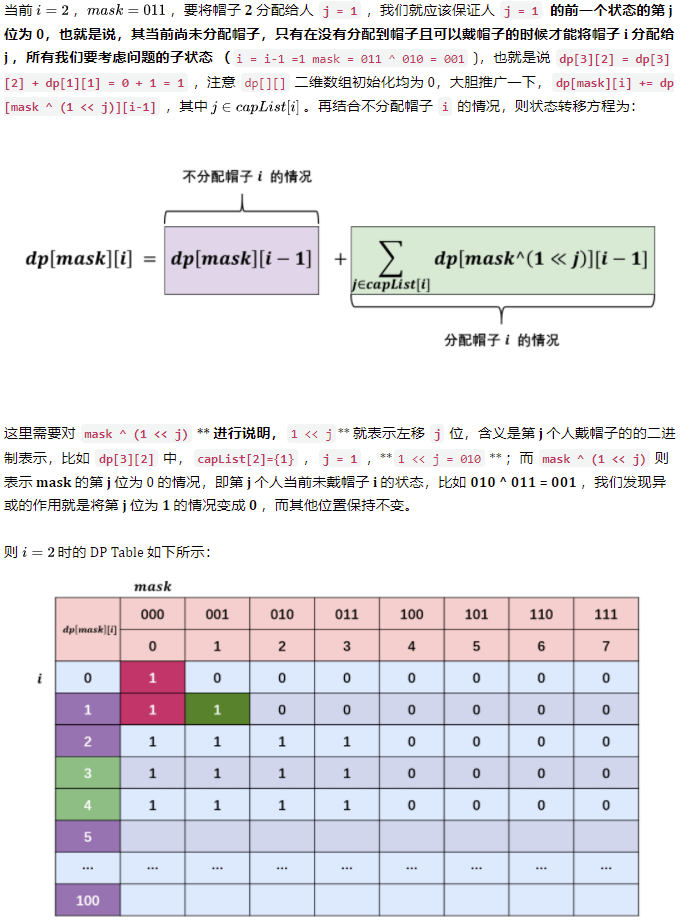
\includegraphics[width=.9\linewidth]{./pic/hats.png}

\begin{minted}[frame=lines,fontsize=\scriptsize,linenos=false]{java}
public int numberWays(List<List<Integer>> hats) {
    int n = hats.size(), range = 1 << n, mod = (int)1e9 + 7;
    List<Integer> ids = new ArrayList<>();
    Map<Integer, List<Integer>> hm = new HashMap<>(); // hats map
    for (int i = 0; i < n; i++) 
        for (int j = 0; j < hats.get(i).size(); j++) {
            hm.computeIfAbsent(hats.get(i).get(j), k -> new ArrayList<>());
            hm.get(hats.get(i).get(j)).add(i);
            if (!ids.contains(hats.get(i).get(j))) ids.add(hats.get(i).get(j));
        }
   int [][] dp = new int [range][ids.size()+1];
   dp[0][0] = 1; // 回到dp[0][0]状态时为1个方案数!
    for (int i = 1; i <= ids.size(); i++) 
        for (int mask = 0; mask < range; mask++) {
            dp[mask][i] = dp[mask][i-1];     // 1.第i个帽子不分配的情况
            int size = hm.get(ids.get(i-1)).size();
            for (int j = 0; j < size; j++)   // 2.第i个帽子分给第j个人的情况
                if ((mask & (1 << hm.get(ids.get(i-1)).get(j))) != 0) {
                    dp[mask][i] += dp[mask ^ (1 << hm.get(ids.get(i-1)).get(j))][i-1]; // 第i个帽子可以是由右边异或的状态转移过来的
                    dp[mask][i] %= mod;
                }
        }
    return dp[range-1][ids.size()];
}
\end{minted}
\section{1595. Minimum Cost to Connect Two Groups of Points - Hard 自顶向下(dfs + 记忆数组);自底向上:DP table}
\label{sec-11-14}
You are given two groups of points where the first group has size1 points, the second group has size2 points, and size1 >= size2.

The cost of the connection between any two points are given in an size1 x size2 matrix where cost[i][j] is the cost of connecting point i of the first group and point j of the second group. The groups are connected if each point in both groups is connected to one or more points in the opposite group. In other words, each point in the first group must be connected to at least one point in the second group, and each point in the second group must be connected to at least one point in the first group.

Return the minimum cost it takes to connect the two groups.
\begin{minted}[frame=lines,fontsize=\scriptsize,linenos=false]{java}
// Staightforward top-down DP for the first group. At the same time, we track which elements from the second group were connected in mask.
// After finishing with the first group, we detect elements in group 2 that are still disconnected,
// and connect them with the "cheapest" node in the first group.
private int dfs(List<List<Integer>> arr, int i, int mask, int [] minCost) { // 自顶向下,需要记忆
    if (dp[i][mask] != null) return dp[i][mask];
    // if (i == m && Integer.bitCount(mask) == n) return 0; // 这行可要可不要
    if (i == m) {       
        int res = 0;
        for (int j = 0; j < n; j++) 
            if ((mask  & (1 << j)) == 0) res += minCost[j];
        return dp[i][mask] = res;
    }
    int res = Integer.MAX_VALUE;
    for (int j = 0; j < n; j++) // 只有暴力查找尝试了所有可能性,才是全局最优解
        res = Math.min(res, dfs(arr, i+1, mask | (1 << j), minCost) + arr.get(i).get(j));
    return dp[i][mask] = res;
}
Integer [][] dp; // (number of points assigned in first group, bitmask of points assigned in second group).
int m, n;
public int connectTwoGroups(List<List<Integer>> cost) {
    m = cost.size();
    n = cost.get(0).size();
    dp = new Integer [m+1][1 << n]; // 右边点组过程中共有1 << n种状态,但是如何知道记住右边的点分别是与左边哪个点连接起来的呢?
    int [] minCost = new int [n];   // 对右边的每个点,它们分别与左边点连通,各点所需的最小花费
    Arrays.fill(minCost, Integer.MAX_VALUE);
    for (int j = 0; j < n; j++) 
        for (int i = 0; i < m; i++) 
            minCost[j] = Math.min(minCost[j], cost.get(i).get(j));
    return dfs(cost, 0, 0, minCost);
}
\end{minted}
\begin{itemize}
\item 动态规划,用二进制压缩状态,注意分析几种情况,就能推出来正确的状态转移方程。
\end{itemize}
\begin{minted}[frame=lines,fontsize=\scriptsize,linenos=false]{java}
public int connectTwoGroups(List<List<Integer>> cost) { 
    int m = cost.size();
    int n = cost.get(0).size();
    int [][] dp = new int [m][1 << n]; // 右边点组过程中共有1 << n种状态,但是如何知道记住右边的点分别是与左边哪个点连接起来的呢?
    for (int i = 0; i < m; i++) 
        Arrays.fill(dp[i], Integer.MAX_VALUE/2);
    for (int i = 0; i < m; i++) {      // 暴力求解所有值取最小
        for (int j = 0; j < 1 << n; j++) {
            for (int k = 0; k < n; k++) {
                if (i > 0 && dp[i-1][j^(1 << k)] != Integer.MAX_VALUE/2) 
                    dp[i][j] = Math.min(dp[i][j], cost.get(i).get(k) + dp[i-1][j ^ (1 << k)]);
                if (i > 0 && dp[i-1][j] != Integer.MAX_VALUE/2)
                    dp[i][j] = Math.min(dp[i][j], cost.get(i).get(k) + dp[i-1][j]);
                if (i == 0 && (j ^ (1 << k)) == 0) dp[i][j] = cost.get(i).get(k);
                else if (dp[i][j^(1 << k)] != Integer.MAX_VALUE/2)
                    dp[i][j] = Math.min(dp[i][j], cost.get(i).get(k) + dp[i][j ^ (1 << k)]);
            }
        }
    }
    return dp[m-1][(1 << n)-1];
}
\end{minted}
\subsection{自顶向下与自底向上}
\label{sec-11-14-1}
以前写dfs的时候总是会忘记记忆数组,现在明白为什么需要记忆以避免重复操作

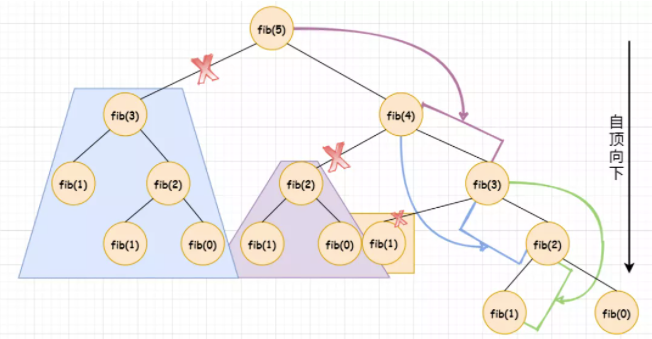
\includegraphics[width=.9\linewidth]{./pic/topDownfib.png}

在两种方法的比较里,自顶向下最下层的操作就转化为自底向上最底层的相关处理,注意两种方法里的不同与相互转换

\section{1755. Closest Subsequence Sum - Hard 分成两半:由O(2$^{\text{N}}$)降为O(NlogN)}
\label{sec-11-15}
You are given an integer array nums and an integer goal.

You want to choose a subsequence of nums such that the sum of its elements is the closest possible to goal. That is, if the sum of the subsequence's elements is sum, then you want to minimize the absolute difference abs(sum - goal).

Return the minimum possible value of abs(sum - goal).

Note that a subsequence of an array is an array formed by removing some elements (possibly all or none) of the original array.
\begin{minted}[frame=lines,fontsize=\scriptsize,linenos=false]{java}
public int minAbsDifference(int[] arr, int goal) {
    int n = arr.length;
    List<Integer> lsum = new ArrayList<>();
    List<Integer> rsum = new ArrayList<>();
    lsum.add(0);
    rsum.add(0);
    for (int i = 0; i <= n/2; i++) { // 这种生成和的方式, i < n/2
        int size = lsum.size();
        for (int j = 0; j < size; j++) 
            lsum.add(lsum.get(j) + arr[i]);
    }
    for (int i = n/2+1; i < n; i++) { // int i = n/2 同样可以,只是左右大小的细微差别
        int size = rsum.size();
        for (int j = 0; j < size; j++) 
            rsum.add(rsum.get(j) + arr[i]);
    }
    TreeSet<Integer> rightSumSet = new TreeSet<>(rsum);
    Set<Integer> leftSumSet = new HashSet<>(lsum);
    int ans = Math.abs(goal);
    for (int v : leftSumSet) {
        int b = goal - v;
        Integer lower = rightSumSet.floor(b); // 对treeset的这几个函数总是记不住
        Integer higher = rightSumSet.ceiling(b);
        if (lower != null)
            ans = Math.min(ans, Math.abs(goal-v-lower));
        if (higher != null)
            ans = Math.min(ans, Math.abs(goal-v-higher));
    }
    return ans;
}
\end{minted}
\begin{itemize}
\item 另一种我都怀疑是不是自己写出来的,居然会忘了。。。。。。
\end{itemize}
\begin{minted}[frame=lines,fontsize=\scriptsize,linenos=false]{java}
// 要把这种工具方法像写binarySearch一样随手拈来随手就敲才行: 仍然超时,最后两个不过
public void getSum(List<Integer> li, int [] arr, int sum , int l, int r) {
    if (l >= r) { //
        li.add(sum);
        return;
    }
    getSum(li, arr, sum + arr[l], l+1, r); // choose and add idx l to sum
    getSum(li, arr, sum, l+1, r);          // skip idx l, move directly to next element
}
public int minAbsDifference(int[] arr, int goal) {
    int n = arr.length, m = arr.length / 2;
    List<Integer> l = new ArrayList<>();
    List<Integer> r = new ArrayList<>();
    getSum(l, arr, 0, 0, m); // m 
    getSum(r, arr, 0, m, n); // m ? 这里反而想不明白了?
    Collections.sort(l);
    Collections.sort(r);
    int i = 0, j = r.size()-1, cur = 0;
    int minDiff = Integer.MAX_VALUE;
    while (i < l.size() && j >= 0) {
        cur = l.get(i) + r.get(j) - goal;
        if (cur > 0) {
            minDiff = Math.min(minDiff, cur);
            j--;
        } else if (cur < 0) {
            minDiff = Math.min(minDiff, -cur);
            i++;
        }
        else return 0;
    }
    return minDiff;
}
\end{minted}
\begin{itemize}
\item Horowitz and Sahni's Subset Sum | comments | links
\begin{itemize}
\item \url{https://leetcode.com/problems/closest-subsequence-sum/discuss/1055432/Java-252ms-or-47.4-MB-or-Horowitz-and-Sahni's-Subset-Sum-or-comments-or-links}
\end{itemize}
\item 好像还有一个类似提交python关于子集的位操作的java方法,回头再找来参考一下
\end{itemize}

\section{2035. Partition Array Into Two Arrays to Minimize Sum Difference - Hard 上一题:分成两半的套娃题}
\label{sec-11-16}
You are given an integer array nums of 2 * n integers. You need to partition nums into two arrays of length n to minimize the absolute difference of the sums of the arrays. To partition nums, put each element of nums into one of the two arrays.

Return the minimum possible absolute difference.
\begin{minted}[frame=lines,fontsize=\scriptsize,linenos=false]{java}
public int minimumDifference(int[] nums) {
    int n = nums.length;
    int sum = Arrays.stream(nums).sum();
    TreeSet<Integer>[] sets = new TreeSet[n/2+1]; // 数组,而不是hashMap,这个应该关系不是很大
    for (int i = 0; i < (1 << (n / 2)); ++i) {    // 一次遍历,而不是n次遍历
        int curSum = 0;
        int m = 0; // element Cnts                         
        for (int j = 0; j < n / 2; ++j) 
            if ((i & (1<<j)) != 0) {
                curSum += nums[j]; // 左半部分
                m ++;
            }
        if (sets[m] == null) sets[m] = new TreeSet<Integer>();
        sets[m].add(curSum);
    }

    int res = Integer.MAX_VALUE;
    for (int i = 0; i < (1 << (n / 2)); ++i) {
        int curSum = 0;
        int m = 0;
        for (int j = 0; j < n / 2; ++j) 
            if ((i & (1<<j)) != 0) {
                curSum += nums[n/2 + j]; // 遍历计算右半部分的和:边遍历,边解决问题
                m ++;
            }
        int target = (sum - 2 * curSum) / 2;
        Integer left = sets[n/2-m].floor(target), right = sets[n/2-m].ceiling(target);
        if (left != null) 
            res = Math.min(res, Math.abs(sum - 2 * (curSum + left.intValue())));
        if (right != null) 
            res = Math.min(res, Math.abs(sum - 2 * (curSum + right.intValue())));
        if (res == 0) return 0;
    }
    return res;
}
\end{minted}
\begin{itemize}
\item 做题的时候有想起tallest billboard,但因为有负数,就去想别的了,却忘记了上面那个一分为二的经典题型
\end{itemize}

\chapter{sliding window}
\label{sec-12}
\section{1438. Longest Continuous Subarray With Absolute Diff Less Than or Equal to Limit - Medium 双端队列}
\label{sec-12-1}
Given an array of integers nums and an integer limit, return the size of the longest non-empty subarray such that the absolute difference between any two elements of this subarray is less than or equal to limit.

\begin{itemize}
\item 这道题希望有一个用两个双端队列的解法,补出来
\end{itemize}

\begin{minted}[frame=lines,fontsize=\scriptsize,linenos=false]{java}
public class MaxSeg {
    List<Integer> tree = new ArrayList<>();
    int n;
    public MaxSeg (int [] arr) {
        n = arr.length;
        tree = new ArrayList<>(2 * n);
        for (int i = 0; i < n; i++)
            tree.add(0);
        for (int i = 0; i < n; i++)
            tree.add(arr[i]); // same effect as below
        for (int i = n-1; i >= 0; i--) // i >= 0
            tree.set(i, Math.max(tree.get(2 * i), tree.get(2 * i+1)));
    }
    public void update(int idx, int v) {
        idx += n;
        tree.set(idx, v);
        while (idx > 1) {
            idx /= 2;
            tree.set(idx, Math.max(tree.get(2 * idx), tree.get(2 * idx+1)));
        }
    }
    public int getMax(int l, int r) {
        l += n;
        r += n;
        int max = Integer.MIN_VALUE;
        while (l < r) {
            if ((l & 1) == 1) {
                max = Math.max(max, tree.get(l));
                l++;
            }
            if ((r & 1) == 1) {
                r--; // order matters !!!
                max = Math.max(max, tree.get(r));
            }
            l >>= 1;
            r >>= 1;
        }
        return max;
    }
}        
public class MinSeg {
    List<Integer> tree = new ArrayList<>();
    int n;
    public MinSeg (int [] arr) {
        n = arr.length;
        tree = new ArrayList<>(2*n);
        for (int i = 0; i < n; i++) 
            tree.add(0);
        for (int i = 0; i < n; i++) 
            tree.add(arr[i]); 
        for (int i = n-1; i >= 0; i--)  // i >= 0
            tree.set(i,  Math.min(tree.get(2*i),  tree.get(2*i+1)));
    }
    public void update(int idx,  int v) {
        idx += n;
        tree.set(idx,  v);
        while (idx > 1) {
            idx /= 2;
            tree.set(idx,  Math.min(tree.get(2*idx),  tree.get(2*idx+1)));
        }
    }
    public int getMin(int l,  int r) { // [l, r) include left, not included right
        l += n;
        r += n;
        int min = Integer.MAX_VALUE;
        while (l < r) {
            if ((l & 1) == 1) {
                min = Math.min(min,  tree.get(l));
                l++;
            }
            if ((r & 1) == 1) {
                r--; // order matters !!!
                min = Math.min(min,  tree.get(r));
            }
            l >>= 1;
            r >>= 1;
        }
        return min;
    }
}
public int longestSubarray(int[] arr, int limit) { // 单调递增队列,左小右大,右进左出 
    MaxSeg max = new MaxSeg(arr);
    MinSeg min = new MinSeg(arr);
    int res = 0, tmp = 0, j = 0;
    int n = arr.length;
    for (int i = 1; i <= n; i++) {
        if (max.getMax(j, i) - min.getMin(j, i) <= limit) {
            tmp = i-j;
            res = Math.max(res, tmp);
        } else 
            while (max.getMax(j, i) - min.getMin(j, i) > limit && j < i) ++j;
    }
    return res;
}
\end{minted}
\section{862. Shortest Subarray with Sum at Least K - Hard}
\label{sec-12-2}
Given an integer array nums and an integer k, return the length of the shortest non-empty subarray of nums with a sum of at least k. If there is no such subarray, return -1.

A subarray is a contiguous part of an array.
\begin{minted}[frame=lines,fontsize=\scriptsize,linenos=false]{java}
public int shortestSubarray(int[] nums, int k) { 
    int n = nums.length;
    int [] sum = new int[n+1];  
    for (int i = 1; i <= n; i++)  
        sum[i] = nums[i-1] + sum[i-1];
    int res = n + 1;
    ArrayDeque<Integer> q = new ArrayDeque<>(); // decreasing sum [] deque
    for (int i = 0; i <= n; i++) {
        while (!q.isEmpty() && sum[i] - sum[q.peekFirst()] >= k)  // 左出:
            res = Math.min(res, i - q.pollFirst()); // 取值了      // 取解
        while (!q.isEmpty() && sum[q.peekLast()] >= sum[i])       // 右出
            q.pollLast();  
        q.offerLast(i);                                           // 当前元素进队列
    }
    return res <= n ? res : -1;
}
\end{minted}

\section{1425. Constrained Subsequence Sum - Hard}
\label{sec-12-3}
Given an integer array nums and an integer k, return the maximum sum of a non-empty subsequence of that array such that for every two consecutive integers in the subsequence, nums[i] and nums[j], where i < j, the condition j - i <= k is satisfied.

A subsequence of an array is obtained by deleting some number of elements (can be zero) from the array, leaving the remaining elements in their original order.

\section{239. Sliding Window Maximum - Hard}
\label{sec-12-4}
You are given an array of integers nums, there is a sliding window of size k which is moving from the very left of the array to the very right. You can only see the k numbers in the window. Each time the sliding window moves right by one position.

Return the max sliding window.

\begin{minted}[frame=lines,fontsize=\scriptsize,linenos=false]{java}
public int[] maxSlidingWindow(int[] arr, int k) {
    int n = arr.length, startWindowIdx = 0;
    ArrayDeque<Integer> q = new ArrayDeque<>(); // 维持一个递减队列
    int [] ans = new int [n - k + 1];
    for (int i = 0; i < n; i++) {
        startWindowIdx = i-k+1;
        while (!q.isEmpty() && i - q.peekFirst() >= k) q.pollFirst();     // 左出q:maintain k size window, 去头:去掉k windows之外的元素
        while (!q.isEmpty() && arr[q.peekLast()] <= arr[i]) q.pollLast(); // 右出q:去掉递减队列尾部所有不大于当前值的元素,就留一个最大值也行
        q.offerLast(i);  // 进q:进后此时q.size() == k 
        if (startWindowIdx >= 0)
            ans[startWindowIdx] = arr[q.peekFirst()]; // 使用递减队列左端最大值
    }
    return ans;
}
\end{minted}
\begin{itemize}
\item 线段树的做法
\end{itemize}
\begin{minted}[frame=lines,fontsize=\scriptsize,linenos=false]{java}
// https://blog.csdn.net/Yaokai_AssultMaster/article/details/79599809
public class MaxSeg {
    List<Integer> tree = new ArrayList<>();
    int n;
    public MaxSeg (int [] arr) {
        n = arr.length;
        tree = new ArrayList<>(2*n);
        for (int i = 0; i < n; i++) 
            tree.add(0);
        for (int i = 0; i < n; i++) 
            tree.add(arr[i]); // same effect as below
        for (int i = n-1; i >= 0; i--) // i >= 0
            tree.set(i, Math.max(tree.get(2*i), tree.get(2*i+1)));
    }
    public void update(int idx, int v) {
        idx += n;
        tree.set(idx, v);
        while (idx > 1) {
            idx /= 2;
            tree.set(idx, Math.max(tree.get(2*idx), tree.get(2*idx+1)));
        }
    }
    public int getMax(int l, int r) {
        l += n;
        r += n;
        int max = Integer.MIN_VALUE;
        while (l < r) {
            if ((l & 1) == 1) {
                max = Math.max(max, tree.get(l));
                l++;
            }
            if ((r & 1) == 1) {
                r--;            // order matters !!!
                max = Math.max(max, tree.get(r));
            }
            l >>= 1;
            r >>= 1;
        }
        return max;
    }
}
public int[] maxSlidingWindow(int[] arr, int k) {
    int n = arr.length;
    MaxSeg mat = new MaxSeg(arr);
    if (n == k) return new int [] {mat.getMax(0, n)};
    int [] res = new int [n-k+1];
    for (int i = 0; i+k <= n; i++) 
        res[i] = mat.getMax(i, i+k);
    return res;
}
\end{minted}

\section{76. Minimum Window Substring}
\label{sec-12-5}
Given two strings s and t of lengths m and n respectively, return the minimum window substring of s such that every character in t (including duplicates) is included in the window. If there is no such substring, return the empty string "".
The testcases will be generated such that the answer is unique.
A substring is a contiguous sequence of characters within the string.
\begin{minted}[frame=lines,fontsize=\scriptsize,linenos=false]{java}
private boolean satisfies(Map<Character, Integer> s, Map<Character, Integer> t) {
    if (s.size() < t.size()) return false;
    for (Map.Entry<Character, Integer> en : t.entrySet()) {
        if (!s.containsKey(en.getKey()) || s.containsKey(en.getKey()) && s.get(en.getKey()) < en.getValue()) return false;
    }
    return true;
}
public String minWindow(String s, String t) {
    int m = s.length();
    int n = t.length();
    if (m < n) return "";
    if (m == 1 && n == 1 && s.charAt(0) != t.charAt(0)) return "";
    if (n == 1) {
        boolean contains = false;
        for (char c : s.toCharArray()) {
            if (c == t.charAt(0)) {
                contains = true;
                break;
            }
        }
        return !contains ? "" : t;
    } 
    Map<Character, Integer> mt = new HashMap<>();
    for (char c : t.toCharArray()) 
        mt.put(c, mt.getOrDefault(c, 0) + 1);
    Map<Character, Integer> ms = new HashMap<>();
    int l = 0, r = 0, i = 0, j = 0, pl = 0;
    String res = "", tmp = "";
    while (i < m) {
        while (i < m && !satisfies(ms, mt)) {
            ms.put(s.charAt(i), ms.getOrDefault(s.charAt(i), 0) + 1);
            ++i;
        }
        if (satisfies(ms, mt)) {
            tmp = s.substring(l, i);
            if (res.equals("") || res.length() > tmp.length()) res = tmp;
        }
        pl = l;
        while (l < i && satisfies(ms, mt)) {
            System.out.println("\nl: " + l);

            ms.put(s.charAt(l), ms.get(s.charAt(l))- 1);
            if (ms.get(s.charAt(l)) == 0) ms.remove(s.charAt(l));
            ++l;
        }
        if (satisfies(ms, mt) || pl != l) {
            tmp = s.substring(l-1, i);
            if (res.equals("") || res.length() > tmp.length()) res = tmp;
        }
        if (i == m) break;
    }
    return res;
}
\end{minted}
\section{632. Smallest Range Covering Elements from K Lists}
\label{sec-12-6}
You have k lists of sorted integers in non-decreasing order. Find the smallest range that includes at least one number from each of the k lists.
We define the range [a, b] is smaller than range [c, d] if b - a < d - c or a < c if b - a == d - c.
\begin{minted}[frame=lines,fontsize=\scriptsize,linenos=false]{java}
// 时间复杂度:O(nk \log k)O(nklogk),其中 nn 是所有列表的平均长度,kk 是列表数量。所有的指针移动的总次数最多是 nknk 次,每次从堆中取出元素和添加元素都需要更新堆,时间复杂度是 O(\log k)O(logk),因此总时间复杂度是 O(nk \log k)O(nklogk)。
// 空间复杂度:O(k)O(k),其中 kk 是列表数量。空间复杂度取决于堆的大小,堆中维护 kk 个元素。
public int[] smallestRange(List<List<Integer>> nums) {
    int n = nums.size();
    int resMin = 0, resMax = Integer.MAX_VALUE;
    int minRg = resMax - resMin;
    int max = Integer.MIN_VALUE;
    int [] next = new int [n]; // 各子链表中比当前idx位数值大的下一个数的下标,即idx+1,初始化全为0
    Queue<Integer> q = new PriorityQueue<>(new Comparator<Integer>() {
            public int compare(Integer idx1, Integer idx2) {
                return nums.get(idx1).get(next[idx1]) - nums.get(idx2).get(next[idx2]);
            }
        });
    for (int i = 0; i < n; i++) {
        q.offer(i); // 0, 1, 2, .... n-1 真神奇呀
        max = Math.max(max, nums.get(i).get(0));
    }
    int minIdx = 0, curRg = 0;
    while (true) {
        minIdx = q.poll(); // 取出的是最小值的子链表的序号,而子链表里的当前最小值所在子链表中的位置存于next[minIdx]中
        curRg = max - nums.get(minIdx).get(next[minIdx]);
        if (curRg < minRg)  {
            minRg = curRg;
            resMin = nums.get(minIdx).get(next[minIdx]);
            resMax = max;
        }
        next[minIdx]++;
        if (next[minIdx] == nums.get(minIdx).size()) break;
        q.offer(minIdx); // 加回去,但是queue里真正比较的值已经变了,变强大了。。。 // 更新最小值的替换值 
        max = Math.max(max, nums.get(minIdx).get(next[minIdx]));  // 更新最大值
    }
    return new int [] {resMin, resMax};
}
// 这里的 BB 序列是什么?我们可以用一个哈希映射来表示 BB 序列—— B[i]
// B[i] 表示 ii 在哪些列表当中出现过,
// 这里哈希映射的键是一个整数,表示列表中的某个数值,
// 哈希映射的值是一个数组,这个数组里的元素代表当前的键出现在哪些列表里。
// 如果列表集合为:
// 0: [-1, 2, 3]
// 1: [1]
// 2: [1, 2]
// 3: [1, 1, 3]
// 那么可以得到这样一个哈希映射
// -1: [0]
// 1: [1, 2, 3, 3]
// 2: [0, 2]
// 3: [0, 3]
public int[] smallestRange(List<List<Integer>> nums) {
    int n = nums.size();
    Map<Integer, List<Integer>> indices = new HashMap<>();
    int xmin = Integer.MAX_VALUE, xmax = Integer.MIN_VALUE;
    for (int i = 0; i < n; i++) {
        for (int v : nums.get(i)) { // 把大链表中出出过的每一个值作键,值为它所存在于的子链表序号链表
            List<Integer> list = indices.getOrDefault(v, new ArrayList<>());
            list.add(i);
            indices.put(v, list);
            xmin = Math.min(xmin, v);
            xmax = Math.max(xmax, v); // 这里得到全局的最小最大值
        }
    }
    int [] freq = new int [n];
    int inside = 0; // cnt # of lists included in miniRanges
    int left = xmin, right = xmin -1;
    int resLeft = xmin, resRight = xmax;
    while (right < xmax) {
        right ++;
        if (indices.containsKey(right)) {
            for (int x : indices.get(right)) {
                freq[x]++;
                if (freq[x] == 1) inside++;
            }
            while (inside == n) { // find ONE satified solution, try to minimize the range
                if (right - left < resRight - resLeft) {
                    resLeft = left;
                    resRight = right;
                }
                if (indices.containsKey(left)) { // sliding the left size towards right
                    for (int v : indices.get(left)) {
                        freq[v]--;
                        if (freq[v] == 0) --inside;
                    }
                }
                left++;
            }
        }
    }
    return new int [] {resLeft, resRight};
}
\end{minted}

\section{480 Sliding Window Median}
\label{sec-12-7}
The median is the middle value in an ordered integer list. If the size of the list is even, there is no middle value. So the median is the mean of the two middle values.
For examples, if arr = [2,3,4], the median is 3.
For examples, if arr = [1,2,3,4], the median is (2 + 3) / 2 = 2.5.
You are given an integer array nums and an integer k. There is a sliding window of size k which is moving from the very left of the array to the very right. You can only see the k numbers in the window. Each time the sliding window moves right by one position.
Return the median array for each window in the original array. Answers within 10-5 of the actual value will be accepted.
\begin{minted}[frame=lines,fontsize=\scriptsize,linenos=false]{java}
public double[] medianSlidingWindow(int[] nums, int k) {
    TreeMap<Integer, Integer> ma = new TreeMap<>();
    TreeMap<Integer, Integer> mb = new TreeMap<>();
    for (int i = 0; i < k; i++) {
        if (i % 2 == 0) {
            mb.put(nums[i], mb.getOrDefault(nums[i], 0) + 1);
            int n = mb.firstKey();
            if (mb.get(n) == 1) mb.remove(n);
            else mb.put(n, mb.get(n) - 1);
            ma.put(n, ma.getOrDefault(n, 0) + 1);
        } else {
            ma.put(nums[i], ma.getOrDefault(nums[i], 0) + 1);
            int n = ma.lastKey();
            if (ma.get(n) == 1) ma.remove(n);
            else ma.put(n, ma.get(n) - 1);
            mb.put(n, mb.getOrDefault(n, 0) + 1);
        }
    }
    double [] res = new double[nums.length-k+1];
    if (k % 2 == 1) res[0] = ma.lastKey();
    else res[0] =  (double)(((long)(ma.lastKey()) + (long)(mb.firstKey())) / 2.0);
    for (int i = 0; i + k < nums.length; i++) {
        ma.put(nums[i+k], ma.getOrDefault(nums[i+k], 0) + 1);
        int n = ma.lastKey();
        if (ma.get(n) == 1) ma.remove(n);
        else ma.put(n, ma.get(n) - 1);
        mb.put(n, mb.getOrDefault(n, 0) + 1);
        if (ma.containsKey(nums[i])) {
            if (ma.get(nums[i]) == 1) ma.remove(nums[i]);
            else ma.put(nums[i], ma.get(nums[i]) - 1);
            int v = mb.firstKey();
            if (mb.get(v) == 1) mb.remove(v);
            else mb.put(v, mb.get(v) - 1);
            ma.put(v, ma.getOrDefault(v, 0) + 1);
        } else {
            if (mb.get(nums[i]) == 1) mb.remove(nums[i]);
            else mb.put(nums[i], mb.get(nums[i]) - 1);
        }
        if (k % 2 == 1) res[i+1] = ma.lastKey();
        else res[i+1] = (double)(((long)(ma.lastKey()) + (long)(mb.firstKey())) / 2.0);
    }
    return res;
}
\end{minted}

\section{826. Most Profit Assigning Work}
\label{sec-12-8}
You have n jobs and m workers. You are given three arrays: difficulty, profit, and worker where:

difficulty[i] and profit[i] are the difficulty and the profit of the ith job, and
worker[j] is the ability of jth worker (i.e., the jth worker can only complete a job with difficulty at most worker[j]).
Every worker can be assigned at most one job, but one job can be completed multiple times.

For example, if three workers attempt the same job that pays \$1, then the total profit will be \$3. If a worker cannot complete any job, their profit is \$0.
Return the maximum profit we can achieve after assigning the workers to the jobs.
\begin{minted}[frame=lines,fontsize=\scriptsize,linenos=false]{java}
// 法一:暴力TreeMap---O(n^2logn)
public int maxProfitAssignment(int[] difficulty, int[] profit, int[] worker) {
    TreeMap<Integer, Integer> m = new TreeMap<>();
    for (int i = 0; i < difficulty.length; i++) 
        m.put(difficulty[i], i);
    int res = 0, idx;
    Integer low;
    for (int i = 0; i < worker.length; i++) {
        low = m.floorKey(worker[i]); // 使用treemap排序的特长
        if (low == null) continue;
        idx = m.get(low);
        for (int j = 0; j < difficulty.length; j++) 
            if (difficulty[j] <= low && profit[j] >= profit[idx])
                idx = j;
        res += profit[idx];
    }
    return res;
}
// 法二:优化的TreeMap---O(nlogn)
// 如果TreeMap里面保存的是每个difficulty[i] 对应的最大的profit,则就可以直接找floorKey对应的value就是对应的要找的value;
// 那么只需要再遍历一次TreeMap,将最大的到目前key位置最大的value放进去就行了
public int maxProfitAssignment(int[] difficulty, int[] profit, int[] worker) {
    TreeMap<Integer, Integer> m = new TreeMap<>();
    for (int i = 0; i < difficulty.length; i++) 
        m.put(difficulty[i], Math.max(m.getOrDefault(difficulty[i], 0), profit[i]));
    int max = 0;
    for (Integer key : m.keySet()) { 
        max = Math.max(max, m.get(key));
        m.put(key, max); //将最大的到目前key位置最大的value放进去
    }
    int res = 0;
    Integer low;
    for (int i = 0; i < worker.length; i++) {
        low = m.floorKey(worker[i]); // 使用treemap排序的特长
        if (low == null) continue;
        res += m.get(low);
    }
    return res;
}
// 法三:Sort + 双指针---O(nlogn)
// 思路就是先将 difficulty[]和profit组成pair,然后再将list和worker[]从小到大排序,然后遍历worker,更新tempMaxProfit,得到总的maxProfit
public int maxProfitAssignment(int[] difficulty, int[] profit, int[] worker) {
    List<int[]> list = new ArrayList<>();
    for (int i = 0; i < difficulty.length; i++) 
        list.add(new int[] {difficulty[i], profit[i]});
    Collections.sort(list, (a, b) -> {return a[0] - b[0];});
    Arrays.sort(worker);
    int res = 0, tmpMaxProfit = 0;
    // i, j同向双指针移动,更新到目前的tmpMaxProfit
    for (int i = 0, j = 0; i < worker.length; i++) {
        while (j < list.size() && list.get(j)[0] <= worker[i]) {
            tmpMaxProfit = Math.max(tmpMaxProfit, list.get(j)[1]);
            j++;
        }
        //此时tmpMaxProfit是前面所有difficulty小于worker[i]的最大的proifit
        res += tmpMaxProfit;
    }
    return res;
}
\end{minted}

\section{1838. Frequency of the Most Frequent Element - Medium}
\label{sec-12-9}
The frequency of an element is the number of times it occurs in an array.

You are given an integer array nums and an integer k. In one operation, you can choose an index of nums and increment the element at that index by 1.

Return the maximum possible frequency of an element after performing at most k operations.

由反证可得,在一定操作次数下最高频元素为原数组中的元素,结合贪心算法,应优先选择不大于该元素的最大数字进行递增操作。

因此,可对原数组排序后,结合双指针算法求解。设计左、右两个指针,在移动右指针的同时,维护左指针的位置,使区间内元素全部递增到右指针所在元素值的操作次数符合要求,此时区间的长度就是该元素的频率。

\begin{minted}[frame=lines,fontsize=\scriptsize,linenos=false]{java}
public int maxFrequency(int[] nums, int k) {
    int n = nums.length, ans = 1, cnt = 0;
    Arrays.sort(nums);
    for (int l = 0, r = 1; r < n; r++) {
        cnt += (nums[r] - nums[r-1]) * (r - l);// 右指针移动后所需操作次数
        while (cnt > k)                        // 操作次数超过k,移动左指针
            cnt -= nums[r] - nums[l++];
        ans = Math.max(ans, r-l+1);            // 区间长度为操作后当前元素的频数
    }
    return ans;
}
\end{minted}

\section{1703. Minimum Adjacent Swaps for K Consecutive Ones - Hard}
\label{sec-12-10}
You are given an integer array, nums, and an integer k. nums comprises of only 0's and 1's. In one move, you can choose two adjacent indices and swap their values.

Return the minimum number of moves required so that nums has k consecutive 1's.

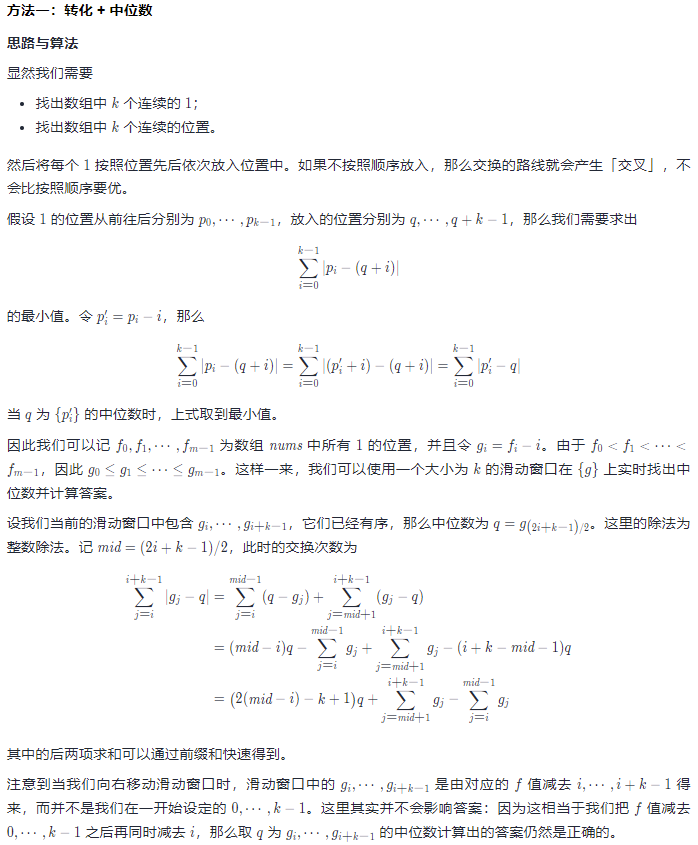
\includegraphics[width=.9\linewidth]{./pic/median.png}

\begin{minted}[frame=lines,fontsize=\scriptsize,linenos=false]{java}
public int minMoves(int[] arr, int k) {
    if (k == 1) return 0;
    int n = arr.length;
    List<Integer> g = new ArrayList<>();
    List<Integer> sum = new ArrayList<>();
    sum.add(0);
    int cnt = -1, last = 0;
    for (int i = 0; i < n; i++) {
        if (arr[i] == 0) continue;
        ++cnt;
        g.add(i-cnt);
        sum.add(last + i - cnt);
        last += i - cnt; 
    }
    int m = g.size();
    int ans = Integer.MAX_VALUE;
    for (int i = 0; i+k <= m; i++) {
        int mid = (i + i + k - 1) / 2; // 中位数下标
        int q = g.get(mid);            // 中位数
        ans = Math.min(ans, (2*(mid-i)-k+1) * q + sum.get(i+k) - sum.get(mid+1) - sum.get(mid) + sum.get(i));
    }
    return ans;
}
\end{minted}
\section{220. Contains Duplicate III - Medium}
\label{sec-12-11}
Given an integer array nums and two integers k and t, return true if there are two distinct indices i and j in the array such that abs(nums[i] - nums[j]) <= t and abs(i - j) <= k.
\begin{minted}[frame=lines,fontsize=\scriptsize,linenos=false]{java}
public boolean containsNearbyAlmostDuplicate(int [] arr, int k, int t) {
    TreeSet<Long> ts = new TreeSet<>();
    for (int i = 0; i < arr.length; i++) {
        if (i >= k+1) ts.remove((long)arr[i-k-1]);
        Long lower = ts.ceiling((long)arr[i]-t); // E ceiling(E e) ,返回 treeSet 中大于等于 e 的元素中最小的元素,如果没有大于等于 e 的元素就返回 null
        if (lower != null && lower <= (long)arr[i] + t)
            return true;
        ts.add((long)arr[i]);
    }
    return false;
}
// 维持一个长度为k的window, 每次检查新的值是否与原来窗口中的所有值的差值有小于等于t的. 如果用两个for循环会超时O(nk).
//     使用treeset( backed by binary search tree) 的subSet函数,可以快速搜索. 复杂度为 O(n logk)
public boolean containsNearbyAlmostDuplicate(int[] nums, int k, int t) {
    if (k < 1 || t < 0 || nums == null || nums.length < 2) return false;
    SortedSet<Long> set = new TreeSet<Long>();
    for(int j = 0; j < nums.length; j++) {
        SortedSet<Long> subSet = set.subSet((long)nums[j] - t, (long)nums[j] + t + 1);
        if (!subSet.isEmpty()) return true;
        if (j >= k)  set.remove((long)nums[j - k]);
        set.add((long)nums[j]);
    }
    return false;
}
\end{minted}


\chapter{backTracking 回溯}
\label{sec-13}
\section{491. Increasing Subsequences}
\label{sec-13-1}
Given an integer array nums, return all the different possible increasing subsequences of the given array with at least two elements. You may return the answer in any order.

The given array may contain duplicates, and two equal integers should also be considered a special case of increasing sequence.
\begin{minted}[frame=lines,fontsize=\scriptsize,linenos=false]{java}
private void dfs(int [] arr, int idx, List<Integer> l) {
    if (l.size() >= 2)
        res.add(new ArrayList<>(l));
    Set<Integer> vis = new HashSet<>();
    for (int i = idx; i < arr.length; i++) {
        if (vis.contains(arr[i])) continue;
        if (l.size() == 0 || arr[i] >= l.get(l.size()-1)) {
            vis.add(arr[i]);
            l.add(arr[i]);
            dfs(arr, i+1, l);
            l.remove(l.size()-1);
        }
    }
}
List<List<Integer>> res = new ArrayList<>();
public List<List<Integer>> findSubsequences(int[] arr) {
    if (arr == null || arr.length == 0) return res;
    dfs(arr, 0, new ArrayList<Integer>());
    return res;
}
\end{minted}


\chapter{排序与recursion}
\label{sec-14}

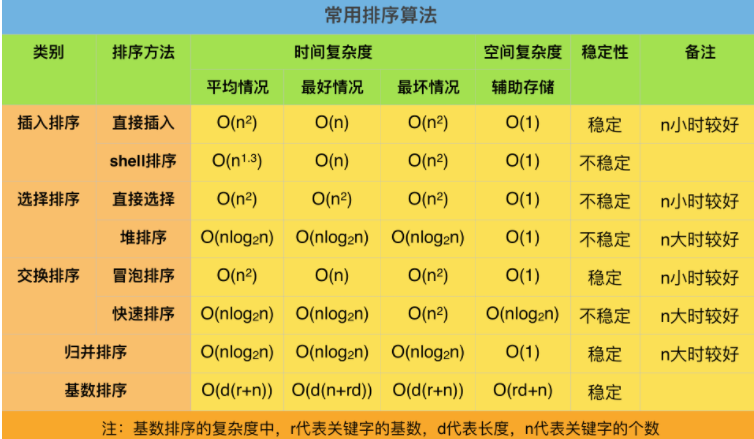
\includegraphics[width=.9\linewidth]{./pic/sort.png}

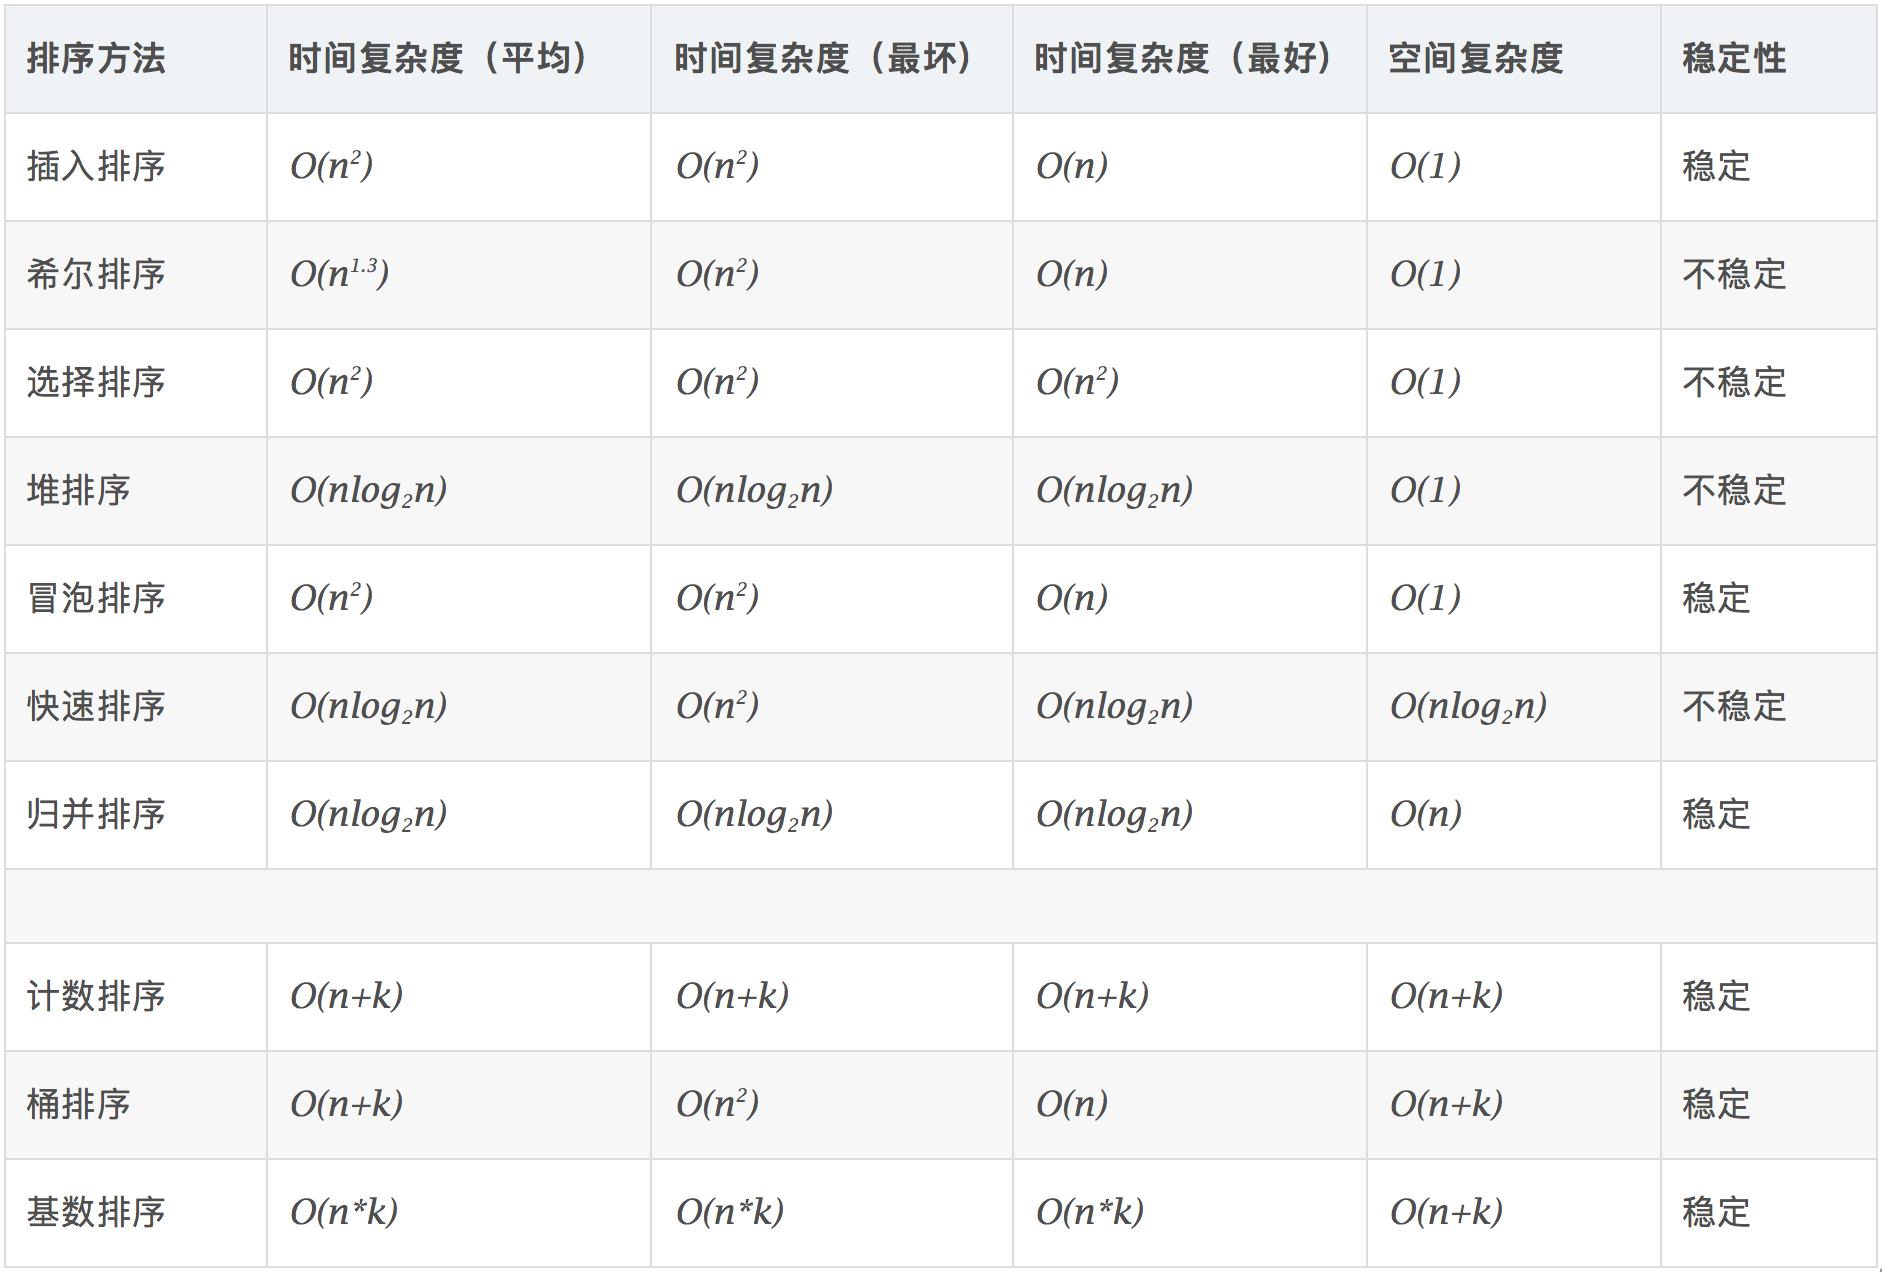
\includegraphics[width=.9\linewidth]{./pic/sort2.png}

\section{1996. The Number of Weak Characters in the Game 桶排序}
\label{sec-14-1}
You are playing a game that contains multiple characters, and each of the characters has two main properties: attack and defense. You are given a 2D integer array properties where properties[i] = [attacki, defensei] represents the properties of the ith character in the game.
A character is said to be weak if any other character has both attack and defense levels strictly greater than this character's attack and defense levels. More formally, a character i is said to be weak if there exists another character j where attackj > attacki and defensej > defensei.
Return the number of weak characters.
\begin{minted}[frame=lines,fontsize=\scriptsize,linenos=false]{java}
public int numberOfWeakCharacters(int[][] properties) {
    int maxAttrack = 0; // 找到所有士兵中的最大值
    for (int[] p : properties)
        maxAttrack = Math.max(maxAttrack,p[0]);
    // 为每一个攻击创建一个桶的位置
    int[] bucket = new int[maxAttrack + 2];     
    // 在每一个攻击力上找到最大的防御力
    for (int[] p : properties)
        bucket[p[0]] = Math.max(bucket[p[0]],p[1]);
    // 将桶的每一个位置都寻找到大于其攻击力的最大防御数值
    int rightMax = bucket[maxAttrack];
    for (int i = maxAttrack; i >= 0; i--) 
        if (rightMax > bucket[i])
            bucket[i] = rightMax;
        else
            rightMax = bucket[i];
    int ans = 0;
    // 最后遍历p 寻找所有的弱将
    for (int[] p : properties)
        if (bucket[p[0] + 1] > p[1]) ans++;  // 攻击力比当前小兵的攻击力大1的桶的位置存放着最大的防御力,与这个防御作比较可以得到当前小兵是否全面弱
    return ans;
}
public int numberOfWeakCharacters(int[][] properties) {
    int cnt = 0;
    int len = properties.length;
    Arrays.sort(properties, (a, b) -> (a[0] ! =  b[0] ? a[0]-b[0] : b[1]-a[1]));
    int max = properties[len-1][1];
    for(int i = len-1;i> = 0;i--){
        if(properties[i][1] < max)
            cnt++;
        max = Math.max(max,properties[i][1]);
    }
    return cnt;
}
\end{minted}

\section{632. Smallest Range Covering Elements from K Lists}
\label{sec-14-2}
You have k lists of sorted integers in non-decreasing order. Find the smallest range that includes at least one number from each of the k lists.
We define the range [a, b] is smaller than range [c, d] if b - a < d - c or a < c if b - a == d - c.
\begin{minted}[frame=lines,fontsize=\scriptsize,linenos=false]{java}
// 时间复杂度:O(nk \log k)O(nklogk),其中 nn 是所有列表的平均长度,kk 是列表数量。所有的指针移动的总次数最多是 nknk 次,每次从堆中取出元素和添加元素都需要更新堆,时间复杂度是 O(\log k)O(logk),因此总时间复杂度是 O(nk \log k)O(nklogk)。
// 空间复杂度:O(k)O(k),其中 kk 是列表数量。空间复杂度取决于堆的大小,堆中维护 kk 个元素。
public int[] smallestRange(List<List<Integer>> nums) {
    int n = nums.size();
    int resMin = 0, resMax = Integer.MAX_VALUE;
    int minRg = resMax - resMin;
    int max = Integer.MIN_VALUE;
    int [] next = new int [n]; // 各子链表中比当前idx位数值大的下一个数的下标,即idx+1,初始化全为0
    Queue<Integer> q = new PriorityQueue<>(new Comparator<Integer>() {
            public int compare(Integer idx1, Integer idx2) {
                return nums.get(idx1).get(next[idx1]) - nums.get(idx2).get(next[idx2]);
            }
        });
    for (int i = 0; i < n; i++) {
        q.offer(i); // 0, 1, 2, .... n-1 真神奇呀
        max = Math.max(max, nums.get(i).get(0));
    }
    int minIdx = 0, curRg = 0;
    while (true) {
        minIdx = q.poll(); // 取出的是最小值的子链表的序号,而子链表里的当前最小值所在子链表中的位置存于next[minIdx]中
        curRg = max - nums.get(minIdx).get(next[minIdx]);
        if (curRg < minRg)  {
            minRg = curRg;
            resMin = nums.get(minIdx).get(next[minIdx]);
            resMax = max;
        }
        next[minIdx]++;
        if (next[minIdx] == nums.get(minIdx).size()) break;
        q.offer(minIdx); // 加回去,但是queue里真正比较的值已经变了,变强大了。。。 // 更新最小值的替换值 
        max = Math.max(max, nums.get(minIdx).get(next[minIdx]));  // 更新最大值
    }
    return new int [] {resMin, resMax};
}
\end{minted}
\begin{itemize}
\item 另外一种解法的
\end{itemize}
\begin{minted}[frame=lines,fontsize=\scriptsize,linenos=false]{java}
// 这里的 BB 序列是什么?我们可以用一个哈希映射来表示 BB 序列—— B[i]
// B[i] 表示 ii 在哪些列表当中出现过,
// 这里哈希映射的键是一个整数,表示列表中的某个数值,
// 哈希映射的值是一个数组,这个数组里的元素代表当前的键出现在哪些列表里。
// 如果列表集合为:
// 0: [-1, 2, 3]
// 1: [1]
// 2: [1, 2]
// 3: [1, 1, 3]
// 那么可以得到这样一个哈希映射
// -1: [0]
// 1: [1, 2, 3, 3]
// 2: [0, 2]
// 3: [0, 3]
// 时间复杂度:O(nk + |V|)O(nk+∣V∣),其中 nn 是所有列表的平均长度,kk 是列表数量,|V|∣V∣ 是列表中元素的值域,在本题中 |V| \leq 2*10^5∣V∣≤2∗10 
// 5
// 。构造哈希映射的时间复杂度为 O(nk)O(nk),双指针的移动范围为 |V|∣V∣,在此过程中会对哈希映射再进行一次遍历,时间复杂度为 O(nk)O(nk),因此总时间复杂度为 O(nk + |V|)O(nk+∣V∣)。
// 空间复杂度:O(nk)O(nk),即为哈希映射使用的空间。哈希映射的「键」的数量由列表中的元素个数 nknk 以及值域 |V|∣V∣ 中的较小值决定,「值」为长度不固定的数组,但是它们的长度之和为 nknk,因此哈希映射使用的空间为 O(nk)O(nk)。在使用双指针时,还需要一个长度为 nn 的数组,其对应的空间在渐进意义下小于 O(nk)O(nk),因此可以忽略。
public int[] smallestRange(List<List<Integer>> nums) {
    int n = nums.size();
    Map<Integer, List<Integer>> indices = new HashMap<>();
    int xmin = Integer.MAX_VALUE, xmax = Integer.MIN_VALUE;
    for (int i = 0; i < n; i++) {
        for (int v : nums.get(i)) { // 把大链表中出出过的每一个值作键,值为它所存在于的子链表序号链表
            List<Integer> list = indices.getOrDefault(v, new ArrayList<>());
            list.add(i);
            indices.put(v, list);
            xmin = Math.min(xmin, v);
            xmax = Math.max(xmax, v); // 这里得到全局的最小最大值
        }
    }
    int [] freq = new int [n];
    int inside = 0; // cnt # of lists included in miniRanges
    int left = xmin, right = xmin -1;
    int resLeft = xmin, resRight = xmax;
    while (right < xmax) {
        right ++;
        if (indices.containsKey(right)) {
            for (int x : indices.get(right)) {
                freq[x]++;
                if (freq[x] == 1) inside++;
            }
            while (inside == n) { // find ONE satified solution, try to minimize the range
                if (right - left < resRight - resLeft) {
                    resLeft = left;
                    resRight = right;
                }
                if (indices.containsKey(left))  // sliding the left size towards right
                    for (int v : indices.get(left)) {
                        freq[v]--;
                        if (freq[v] == 0) --inside;
                    }
                left++;
            }
        }
    }
    return new int [] {resLeft, resRight};
}
\end{minted}

\section{Reverse Pairs}
\label{sec-14-3}
Given an integer array nums, return the number of reverse pairs in the array.
A reverse pair is a pair (i, j) where 0 <= i < j < nums.length and nums[i] > 2 * nums[j].
\begin{minted}[frame=lines,fontsize=\scriptsize,linenos=false]{java}
private int mergeSortCount(long [] arr, int bgn, int end) {
if (bgn >= end) return 0;
int mid = bgn + (end-bgn)/2;
int cnt = mergeSortCount(arr, bgn, mid) + mergeSortCount(arr, mid+1, end);
    for (int i = bgn, j = mid+1; i <= mid; i++) {
        while (j <= end && arr[i] > 2*arr[j]) j++;
        cnt += j - (mid+1);
    }
    Arrays.sort(arr, bgn, end+1);
    return cnt;
}
public int reversePairs(int[] nums) {
    int n = nums.length;
    return mergeSortCount(Arrays.stream(nums).mapToLong(i -> i).toArray(), 0, n-1);
}
// bit 的解法: https://www.cnblogs.com/grandyang/p/6657956.html
\end{minted}

\section{306. Additive Number}
\label{sec-14-4}
Additive number is a string whose digits can form additive sequence.

A valid additive sequence should contain at least three numbers. Except for the first two numbers, each subsequent number in the sequence must be the sum of the preceding two.

Given a string containing only digits '0'-'9', write a function to determine if it's an additive number.

Note: Numbers in the additive sequence cannot have leading zeros, so sequence 1, 2, 03 or 1, 02, 3 is invalid.
\begin{minted}[frame=lines,fontsize=\scriptsize,linenos=false]{java}
public boolean isAdditiveNumber(String num) {
    int n = num.length();
    if (n < 3) return false;
    for (int i = 1; i <= num.length() >> 1; i++)
        for (int j = 1; j + i < num.length(); j++)  
            if (isValid(num, num.substring(0, i), num.substring(i, i + j), i + j)) return true;
    return false;
}
private boolean isValid(String num, String first, String second, int index) {
    if (first.length() > 1 && first.startsWith("0") 
        || second.length() > 1 && second.startsWith("0")) return false;
    if (index == num.length()) return true; // 如果只有两个数是有效的!!!
    long sum = Long.parseLong(first) + Long.parseLong(second);
    if (num.startsWith(sum + "", index)) // 间接检测第三个数
        if (isValid(num, second, sum + "", index + (sum + "").length())) return true;
    return false;
}
\end{minted}


\chapter{dfs}
\label{sec-15}
\section{464. Can I Win}
\label{sec-15-1}
In the "100 game" two players take turns adding, to a running total, any integer from 1 to 10. The player who first causes the running total to reach or exceed 100 wins.
What if we change the game so that players cannot re-use integers?
For example, two players might take turns drawing from a common pool of numbers from 1 to 15 without replacement until they reach a total >= 100.
Given two integers maxChoosableInteger and desiredTotal, return true if the first player to move can force a win, otherwise, return false. Assume both players play optimally.
\begin{minted}[frame=lines,fontsize=\scriptsize,linenos=false]{java}
// state是前走的人走完之后的局面,sum是当前数字总和,返回的是当前走的人是否能赢
private boolean dfs(int max, int target, int state, int val) {
    if (dp[state] != -1) return dp[state] > 0;
    if (val >= target) { // 如果对方取数的时候总和达到target了,则当前走的人输了,做记忆并返回false
        dp[state] = 0;
        return false;
    }
    for (int i = 1; i <= max; i++) {  // 枚举当前人取哪个数
        if ((state >> i-1 & 1) == 0 && !dfs(max, target, state | (1 << i-1), val + i)) {
            dp[state] = 1;
            return true;
        }
    }
    dp[state] = 0;
    return false;
}
int [] dp;
public boolean canIWin(int maxChoosableInteger, int desiredTotal) {
    if (desiredTotal <= maxChoosableInteger) return true;
    if (desiredTotal > (maxChoosableInteger + 1)*maxChoosableInteger / 2) return false;
    dp = new int[1 << maxChoosableInteger]; // 时空复杂度O ( 2 m ) O(2^m)O(2 
    Arrays.fill(dp, -1);
    return dfs(maxChoosableInteger, desiredTotal, 0, 0);
}
\end{minted}


\chapter{排列与组合}
\label{sec-16}
\section{903. Valid Permutations for DI Sequence - Hard}
\label{sec-16-1}
You are given a string s of length n where s[i] is either:

'D' means decreasing, or
'I' means increasing.
A permutation perm of n + 1 integers of all the integers in the range [0, n] is called a valid permutation if for all valid i:

If s[i] \texttt{= 'D', then perm[i] > perm[i + 1], and
If s[i] =} 'I', then perm[i] < perm[i + 1].
Return the number of valid permutations perm. Since the answer may be large, return it modulo 109 + 7.

当是降序时,下一个数字不小于当前最后一个数字,反之是升序时,下一个数字小于当前最后一个数字,所以可以写出状态转移方程如下所示:
\begin{minted}[frame=lines,fontsize=\scriptsize,linenos=false]{java}
if (S[i-1] == 'D')    dp[i][j] += dp[i-1][k]    ( j <= k <= i-1 )
else                  dp[i][j] += dp[i-1][k]    ( 0 <= k < j )
\end{minted}
\begin{minted}[frame=lines,fontsize=\scriptsize,linenos=false]{java}
public int numPermsDISequence(String s) {
    int n = s.length(), mod = (int)1e9 + 7, res = 0;
    int [][] dp = new int [n+1][n+1];
    dp[0][0] = 1;
    for (int i = 1; i <= n; i++) 
        for (int j = 0; j <= i; j++) // 考虑当前最后一个元素为j
            if (s.charAt(i-1) == 'D')
                // 可以把序列中所有大于等于j的元素都加上1得到新序列(这个时候是不会改变当前序列的大小关系的),再把j添加到序列末尾得到
                for (int k = j; k <= i; k++) 
                    dp[i][j] = (dp[i][j] + dp[i-1][k]) % mod;
            else // 考虑当前最后一个元素为j
                // 把该序列中所有大于等于j(k < j <= i)的数字都加上1,并在末尾添加一个j得到dp[i][j]中的一种方案
                for (int k = 0; k < j; k++) // 把序列中所有大等于j的元素都加上1,再把j放在序列末尾得到
                    dp[i][j] = (dp[i][j] + dp[i-1][k]) % mod;
    for (int i = 0; i <= n; i++) 
        res = (res + dp[n][i]) % mod;
    return (int)res;
}
\end{minted}

\section{1467. Probability of a Two Boxes Having The Same Number of Distinct Balls - Hard}
\label{sec-16-2}
Given 2n balls of k distinct colors. You will be given an integer array balls of size k where balls[i] is the number of balls of color i. 

All the balls will be shuffled uniformly at random, then we will distribute the first n balls to the first box and the remaining n balls to the other box (Please read the explanation of the second example carefully).

Please note that the two boxes are considered different. For example, if we have two balls of colors a and b, and two boxes [] and (), then the distribution [a] (b) is considered different than the distribution [b] (a) (Please read the explanation of the first example carefully).

We want to calculate the probability that the two boxes have the same number of distinct balls.

Example: [2, 1, 1]

for first ball, we can put both ball in first bin and 0 ball in second bin OR we can put 1 ball in first bin, second ball in 2nd bin OR we can put both in second bin

for second ball, we can put ball in first bin and 0 ball in second bin, similarly, we can put 1 ball in second bin.

same thing with the third ball

Try all possible permutations recursively. And, in the end check, if there are equal number of distinct balls in both bins or not.

\begin{minted}[frame=lines,fontsize=\scriptsize,linenos=false]{java}
public double getProbability(int[] balls) {
    int sum = Arrays.stream(balls).sum();
    double all = allCases(balls, 0, 0, 0, 0, 0, sum);
    double valid = casesWithEqualDistinctBalls(balls, 0, 0, 0, 0, 0, sum);
    return (1.0 * valid / all);
}
// disF = distinct balls in first bin
// disS = distinct balls in second bin
// f = number of balls in first bin
// s = number of balls in second bin
public double allCases(int [] arr, int pos, int f, int s, int disF, int disS, int sum) {
    if (pos == arr.length) {
        // for all cases, we just need to check if both bins have same number of balls or not
        if (f == s) return fact(sum / 2) * fact(sum / 2); // numerator of our permutations
        return 0;
    }
    // we put all balls in second bin
    double ans = 1.0 * allCases(arr, pos+1, f, s+arr[pos], disF, disS+1, sum) / fact(arr[pos]);
    // we put all balls in first bin
    ans += 1.0 * allCases(arr, pos+1, f+arr[pos], s, disF+1, disS, sum) / fact(arr[pos]);
    for (int i = 1; i < arr[pos]; i++) // 把每一种颜色的球放到两个里面盒子里都有
        ans += 1.0 * allCases(arr, pos+1, f+i, s+arr[pos]-i, disF+1, disS+1, sum) / (fact(i) * fact(arr[pos]-i));
    return ans;
}
public double casesWithEqualDistinctBalls(int [] arr, int pos, int f, int s, int disF, int disS, int sum) {
    if (pos == arr.length) {
        if (f == s && disF == disS) return fact(sum / 2) * fact(sum / 2);
        return 0;
    }
    double ans = 1.0 * casesWithEqualDistinctBalls(arr, pos+1, f, s+arr[pos], disF, disS+1, sum) / fact(arr[pos]);
    ans += 1.0 * casesWithEqualDistinctBalls(arr, pos+1, f+arr[pos], s, disF+1, disS, sum) / fact(arr[pos]);
    for (int i = 1; i < arr[pos]; i++) 
        ans += 1.0 * casesWithEqualDistinctBalls(arr, pos+1, f+i, s+arr[pos]-i, disF+1, disS+1, sum) / (fact(i) * fact(arr[pos]-i));
    return ans;
}
private double fact(double n) {
    double res = 1;
    for (int i = 2; i <= n; i++) 
        res = res * i;
    return res;
}
// Complexity: There can be total of (8 * 6) balls with 8 distinct. Complexity of recursion is f * s * disF * disS = O(48 * 48 * 8 * 8)
\end{minted}


\chapter{Union Find 并查集}
\label{sec-17}
\section{1697. Checking Existence of Edge Length Limited Paths - Hard}
\label{sec-17-1}
An undirected graph of n nodes is defined by edgeList, where edgeList[i] = [ui, vi, disi] denotes an edge between nodes ui and vi with distance disi. Note that there may be multiple edges between two nodes.

Given an array queries, where queries[j] = [pj, qj, limitj], your task is to determine for each queries[j] whether there is a path between pj and qj such that each edge on the path has a distance strictly less than limitj .

Return a boolean array answer, where answer.length == queries.length and the jth value of answer is true if there is a path for queries[j] is true, and false otherwise.
\begin{minted}[frame=lines,fontsize=\scriptsize,linenos=false]{java}
private class DisjointSetUnion {
    private int N;
    private int [] parent, rank;
    public DisjointSetUnion( int n) {
        this.N = n;
        this.parent = new int [N];
        this.rank = new int [N];
        for (int i = 0; i < N; i++) {
            this.parent[i] = i;
            this.rank[i] = 1;
        }
    }
    public boolean areConnected(int u, int v) {
        return find(u) == find(v);
    }
    public void union(int u, int v) { // O(Log(N))
        if (u != v) {
            int p = find(u);
            int q = find(v);
            if (p != q) {
                if (rank[p] > rank[q]) {
                    parent[q] = p;
                    rank[p] += rank[q];
                } else {
                    parent[p] = q;
                    rank[q] += rank[p];
                }
            }
        }
    }
    private int find(int v) { // 我记得这里有个同步更新父数组的优化步骤,和rank优化冲突吗?要总结一下 // O(Log(N))
        int x = v;
        while (x != parent[x])
            x = parent[x];
        parent[v] = x;
        return x;
    }
}
class Query implements Comparable<Query> {
    public int idx, start, end, weight;
    public Query(int idx, int bgn, int end, int weight) {
        this.idx = idx;
        this.start = bgn;
        this.end = end;
        this.weight = weight;
    }
    @Override public int compareTo(Query query) {
        return this.weight - query.weight;
    }
}
// 我们可以分别对 edges 和 queries 进行一次升序排序。本题和 1170. 比较字符串最小字母出现频次 类似, 都可以采取 *离线排序优化* 的方式来解。
// 接下来,遍历 queries。遍历 queries 的同时将权值小于 limitj 的边进行合并。
// 接下来,我们只需要判断 pj 和 qj 是否已经在同一个联通域即可。
// 因此如果 pj 和 qj 在同一个联通域,那么其联通的路径上的所有边必定都小于 limitj,其原因就是前面加粗的那句话。
// 注意到排序打乱了 queries 的索引,因此我们需要记录一下其原始索引。
public boolean[] distanceLimitedPathsExist(int n, int[][] edgeList, int[][] queries) {
    DisjointSetUnion set = new DisjointSetUnion(n);
    Arrays.sort(edgeList, (a, b) -> a[2]-b[2]); // arrange edges in ascending order of weights
    int m = queries.length, i;
    int E = edgeList.length;
    Query [] qarr = new Query[m];
    for (i = 0; i < m; i++) 
        qarr[i] = new Query(i, queries[i][0], queries[i][1], queries[i][2]);
    Arrays.sort(qarr);                // arrange queries in ascending order of threshold weights
    boolean [] ans = new boolean [m];
    int idx = 0;
    for (i = 0; i < m; i++) {
        while (idx < E && edgeList[idx][2] < qarr[i].weight) {
            set.union(edgeList[idx][0], edgeList[idx][1]);
            ++idx;
        }
        ans[qarr[i].idx] = set.areConnected(qarr[i].start, qarr[i].end);
    }
    return ans;
}
// 令 m, q edges 和 queries 的长度。
//     时间复杂度:$O(mlogm + qlogq)
//     空间复杂度:$O(n + q)
// Runtime is bound by sorting: O(ElogE + NlogN + N + E);
\end{minted}

\section{2003. Smallest Missing Genetic Value in Each Subtree - Hard}
\label{sec-17-2}
There is a family tree rooted at 0 consisting of n nodes numbered 0 to n - 1. You are given a 0-indexed integer array parents, where parents[i] is the parent for node i. Since node 0 is the root, parents\footnotemark[2]{} == -1.

There are 105 genetic values, each represented by an integer in the inclusive range [1, 105]. You are given a 0-indexed integer array nums, where nums[i] is a distinct genetic value for node i.

Return an array ans of length n where ans[i] is the smallest genetic value that is missing from the subtree rooted at node i.

The subtree rooted at a node x contains node x and all of its descendant nodes.
\begin{minted}[frame=lines,fontsize=\scriptsize,linenos=false]{java}
private void dfs(int i, Set<Integer> visited, int [] arr) { // 图的遍历:自顶向下ok,自底向上还不太熟悉,需要练习,还有一个没有消化好的类似题,找出来binary indexed tree
    if (!visited.contains(arr[i])) {
        Set<Integer> children = tree.getOrDefault(i, new HashSet<Integer>());
        for (int v : children) 
            dfs(v, visited, arr);
        visited.add(arr[i]);
    }
}
Map<Integer, Set<Integer>> tree = new HashMap<>();
int [] ans;
int n;
public int[] smallestMissingValueSubtree(int[] parents, int[] nums) {
    n = parents.length;
    ans = new int [n];
    Arrays.fill(ans, 1); 
    int oneIdx = -1;
    for (int i = 0; i < n; i++) 
        if (nums[i] == 1) {
            oneIdx = i;
            break;
        }
    if (oneIdx == -1) return ans;
    for (int i = 1; i < n; i++) {
        tree.computeIfAbsent(parents[i], k -> new HashSet<Integer>());
        tree.get(parents[i]).add(i);
        // tree.computeIfAbsent(i, k -> new HashSet<Integer>()); // 这里要想一下:为什么双向图他只加一个方向?
        // tree.get(i).add(parents[i]);
    }
    Set<Integer> visited = new HashSet<>(); // 这个直接转化为想要的结果,很便捷
    int parentIter = oneIdx;
    int miss = 1;
    while (parentIter >= 0) { // 从值为1的节点向根遍历(自底向上),没有任何重复计算,只走完这一条自底向项的路径就可以了
        dfs(parentIter, visited, nums);
        while (visited.contains(miss)) ++miss;
        ans[parentIter] = miss;
        parentIter = parents[parentIter];
    }
    return ans;
}
\end{minted}

\section{803. Bricks Falling When Hit - Hard 反向: 变de-Union vs为 Re-Union}
\label{sec-17-3}
You are given an m x n binary grid, where each 1 represents a brick and 0 represents an empty space. A brick is stable if:

It is directly connected to the top of the grid, or
At least one other brick in its four adjacent cells is stable.
You are also given an array hits, which is a sequence of erasures we want to apply. Each time we want to erase the brick at the location hits[i] = (rowi, coli). The brick on that location (if it exists) will disappear. Some other bricks may no longer be stable because of that erasure and will fall. Once a brick falls, it is immediately erased from the grid (i.e., it does not land on other stable bricks).

Return an array result, where each result[i] is the number of bricks that will fall after the ith erasure is applied.

Note that an erasure may refer to a location with no brick, and if it does, no bricks drop.


\includegraphics[width=.9\linewidth]{./pic/hitBricks.png}

\begin{minted}[frame=lines,fontsize=\scriptsize,linenos=false]{java}
private class UnionFind {
    int [] id; // parent
    int [] cnt;// size
    public UnionFind (int n) {
        id = new int [n];
        cnt = new int [n];
        for (int i = 0; i < n; i++) {
            id[i] = i;
            cnt[i] = 1;
        }
    }
    public int find(int i) {
        while (id[i] != i) {
            id[i] = id[id[i]];
            i = id[i];
        }
        return i;
    }
    public void union(int i, int j) {
        int rootI = find(i);
        int rootJ = find(j);
        if (rootI != rootJ) {
            id[rootI] = rootJ;
            cnt[rootJ] += cnt[rootI];
        }
    }
}
private void unionAround(int x, int y, int [][] arr, UnionFind uf) {
    for (int [] d : dirs) {
        int i = x + d[0];
        int j = y + d[1];
        if (i < 0 || i >= m || j < 0 || j >= n) continue;
        if (arr[i][j] == 1) uf.union(x*n+y+1, i*n+j+1); // +1
    }
    if (x == 0) uf.union(x*n+y+1, 0); // 第一排的直接与顶相连 // trick: to help calculate cnts connecting top easier/faster
}
int [][] dirs = {{1, 0}, {-1, 0}, {0, 1}, {0, -1}};
int m, n;
public int[] hitBricks(int[][] grid, int[][] hits) {
    m = grid.length;
    n = grid[0].length;
    for (int [] hit : hits)              // 首先把所有要打的砖块标记为2.
        if (grid[hit[0]][hit[1]] == 1)   // 如果有砖头
            grid[hit[0]][hit[1]] = 2;
    UnionFind uf = new UnionFind(m*n+1); // 这里的 + 1主要是多一个0来表示顶,所有的第一排的砖在unionfind的时候都会直接与这个0相连。
    for (int i = 0; i < m; i++)          // 然后对打掉后的数组中的砖块进行四个方向的union
        for (int j = 0; j < n; j++) 
            if (grid[i][j] == 1)
                unionAround(i, j, grid, uf);
    int cnt = uf.cnt[uf.find(0)];        // 这个count就是打完后一定会剩下的砖块数量.
    int [] ans = new int [hits.length];
    for (int i = hits.length-1; i >= 0; i--) {
        int [] hit = hits[i];
        if (grid[hit[0]][hit[1]] == 2) { // 对于需要复原的这个砖块做四个方向union,主要是为了得到有多少砖必须通过这块砖才能连接到顶部。
            unionAround(hit[0], hit[1], grid, uf);
            grid[hit[0]][hit[1]] = 1;    // 由于是从后向前,做完要把这块砖重新标记回来: 这些砖是有可能被hits前序砖敲掉后掉落下来的,不复原影响前序结果
        }
        int newCnt = uf.cnt[uf.find(0)];
        ans[i] = (newCnt - cnt > 0 ? newCnt - cnt - 1 : 0);
        cnt = newCnt;
    }
    return ans;
}
\end{minted}

\section{721. Accounts Merge}
\label{sec-17-4}
Given a list of accounts where each element accounts[i] is a list of strings, where the first element accounts[i]\footnotemark[2]{} is a name, and the rest of the elements are emails representing emails of the account.

Now, we would like to merge these accounts. Two accounts definitely belong to the same person if there is some common email to both accounts. Note that even if two accounts have the same name, they may belong to different people as people could have the same name. A person can have any number of accounts initially, but all of their accounts definitely have the same name.

After merging the accounts, return the accounts in the following format: the first element of each account is the name, and the rest of the elements are emails in sorted order. The accounts themselves can be returned in any order.

\begin{itemize}
\item Similar to the most voted solution, my solution uses the index of the owner as the key for the union map, to avoid possible issue caused by different owners have the same name, thus uses one less loop.
\end{itemize}

\begin{minted}[frame=lines,fontsize=\scriptsize,linenos=false]{java}
private int findParent(int [] arr, int x) {
    if (arr[x] == x) return x;
    arr[x] = findParent(arr, arr[x]);
    return arr[x];
}
public List<List<String>> accountsMerge(List<List<String>> accounts) {
    Map<String, Integer> owner = new HashMap<>();
    Map<Integer, TreeSet<String>> union = new HashMap<>(); // match idx & Set<Sting emails>
    int n = accounts.size(), p = 0;
    int [] par = new int [n];
    for (int i = 0; i < n; i++) par[i] = i;
    List<String> ls = new ArrayList<>(); 
    for (int i = 0; i < n; i++) { // find the ownerIdx for each email address
        ls = accounts.get(i);
        for (int j = 1; j < ls.size(); j++) {
            String email = ls.get(j);
            if (owner.containsKey(email)) {
                p = findParent(par, owner.get(email));
                par[p] = i; // union accounts that belong to the same user here by updating parent relation
            }
            owner.put(email, i);
        }
    }
     // union all emails belong to the same owner
    for (String emal : owner.keySet()) {
        int ownerIdx = findParent(par, owner.get(emal));
        TreeSet<String> set = union.getOrDefault(ownerIdx, new TreeSet<>());
        set.add(emal);
        union.put(ownerIdx, set);
    }
// Generate return result
    List<List<String>> res = new ArrayList<>();
    for (int ownerIdx : union.keySet()) {
        ls = new ArrayList<>();
        ls.add(accounts.get(ownerIdx).get(0));  // get the owner name
        ls.addAll(union.get(ownerIdx));
        res.add(ls);
    }
    return res;
}
\end{minted}

\section{1202. Smallest String With Swaps}
\label{sec-17-5}
You are given a string s, and an array of pairs of indices in the string pairs where pairs[i] = [a, b] indicates 2 indices(0-indexed) of the string.

You can swap the characters at any pair of indices in the given pairs any number of times.

Return the lexicographically smallest string that s can be changed to after using the swaps.
\begin{minted}[frame=lines,fontsize=\scriptsize,linenos=false]{java}
int [] par;
int [] rank;
int n;
public int find(int v) {
    if (v != par[v] ) 
        par[v] = find(par[v]);
    return par[v];
}
public boolean union(int i, int j) {
    int ri = find(i);
    int rj = find(j);
    if (ri == rj) return false;
    if (rank[ri] < rank[rj]) par[ri] = rj;
    else if (rank[ri] > rank[rj]) par[rj] = ri;
    else {
        par[rj] = ri;
        rank[ri] ++; // 维护rank的值
    }
    return true;
}
public String smallestStringWithSwaps(String s, List<List<Integer>> pairs) {
    int n = s.length();
    par = new int [n];
    rank = new int [n];
    List<Queue<Character>> list = new ArrayList<>(n);
    for (int i = 0; i < n; i++) {
        par[i] = i;
        list.add(new PriorityQueue<>());
    }
    Arrays.fill(rank, 1);
    pairs.forEach(p -> union(p.get(0), p.get(1))); // Perform union for each pair.
    // Add each character to the priority queue associated with its component.
    IntStream.range(0, n).forEach(index -> list.get(find(index)).add(s.charAt(index)));
    // Build the result, by removing chars from the corresponding priority queue.
    StringBuilder buffer = new StringBuilder(n);
    IntStream.range(0, n).forEachOrdered(index -> buffer.append(list.get(find(index)).remove()));
    return buffer.toString();
}
// O(NlogN). Worst-case, all indices are part of the same component. So we will essentially be popping off from the same priority queue.
// Space Complexity: O(N).
\end{minted}

\section{1998. GCD Sort of an Array - Hard}
\label{sec-17-6}
You are given an integer array nums, and you can perform the following operation any number of times on nums:

Swap the positions of two elements nums[i] and nums[j] if gcd(nums[i], nums[j]) > 1 where gcd(nums[i], nums[j]) is the greatest common divisor of nums[i] and nums[j].
Return true if it is possible to sort nums in non-decreasing order using the above swap method, or false otherwise.
\begin{minted}[frame=lines,fontsize=\scriptsize,linenos=false]{java}
private int find (int v) {
    if (!parent.containsKey(v)) {
        parent.put(v, v);
        return v;
    }
    if (parent.get(v) != v)
        parent.put(v, find(parent.get(v)));
    return parent.get(v);
}
private void union(int x, int y) {
    int rx = find(x);
    int ry = find(y);
    if (rx != ry) parent.put(rx, ry);
}
/**
   general idea (not accepted)
   we can simply union pairs of numbers which has gcd > 1 in quadratic time and then check of groups that
   are formed by union of pairs can be invidually sorted. 
   improved (accpeted)
   In above approach problem is we are union-ing pairs in quadratic time. To improve upon it. We union a number
   which is present in 'nums' with its smallest prime factor. thus if two numbers has same smallest prime factor
   their gcd is guaranted to be > 1. 
**/
Map<Integer, Integer> parent = new HashMap<>();
public boolean gcdSort(int[] arr) {
    int n = arr.length;
    parent = new HashMap<Integer, Integer>();
    int [] sorted = arr.clone();
    Arrays.sort(sorted);
    int max = Arrays.stream(arr).max().getAsInt();
    Set<Integer> numSet = new HashSet<>();
    numSet.addAll(Arrays.stream(arr).boxed().collect(Collectors.toList()));
    int p = 2;  // Seive algorithm
    boolean [] primes = new boolean [max + 1];
    Arrays.fill(primes, true);
    while (p < max) {
        if (primes[p]) {
            for (int i = p; i <= max; i += p) { // 我合并的是数组的索引,他优化成合并所有拥有公约数为p的数组中沿未合并的值
                if (numSet.contains(i)) union(p, i);
                primes[i] = false;
            }
        }
        p++;
    }
    for (int i = 0; i < n; i++) 
        if (arr[i] != sorted[i] && find(sorted[i]) != find(arr[i])) return false;
    return true;
}
\end{minted}

\section{1724 给定一个n nn个顶点的无向带权图,要求在线回答若干询问,每次询问是个三元组( p , q , x ) (p,q,x)(p,q,x),是问是否存在p pp到q qq的每条边都小于x xx的路径。}
\label{sec-17-7}

先以Kruskal算法求最小生成森林,显然对于任何p pp和q qq,它们之间所有路径中最大边最小的那条路径的最大边一定是最小生成树的某条边(如果存在路径的话)。建树完成之后,对每个连通块,以任意顶点为根,将该连通块做成一棵有根树。对于每次询问,我们只需求p pp和q qq所有到它们的最近公共祖先所经过的边的最大边权就行了。可以考虑用倍增思想(以下的内容可以参考\url{https://blog.csdn.net/qq_46105170/article/details/116217633),开两个数组f} ff和g gg,其中f [ i ] [ k ] f[i][k]f[i][k]指的是从i ii节点向上跳2 k 2$^{\text{k2}}$ 
k
 步能过走到的顶点是谁(如果跳出界了则规定值为− 1 -1−1),g [ i ] [ k ] g[i][k]g[i][k]指的是从i ii节点向上跳2 k 2$^{\text{k2}}$ 
k
 的过程中经过的边的最大权值(在不会跳出界的情况下),然后从每个树根做BFS,初始化f [ . ] [ 0 ] f[.]\footnotemark[2]{}f[.]\footnotemark[2]{}和g [ . ] [ 0 ] g[.]\footnotemark[2]{}g[.]\footnotemark[2]{}。由于在询问的时候需要知道最近公共祖先,所以还需要一个数组d dd记录每个顶点的深度,在BFS的时候可以同时求出。接下来,用倍增的思想计算f ff和g gg:
\begin{minted}[frame=lines,fontsize=\scriptsize,linenos=false]{java}
f[i][k] = f[f[i][k-1]][k-1]
g[i][k] = max{g[i][k-1],g[f[i][k-1]][k-1]}
\end{minted}
至此,所有的预处理就完成了。

接下来询问的时候,如果p pp与q qq不连通则直接返回false。否则看一下两个顶点的深度,不妨设p pp更深,则将p pp向上跳若干步,使得p pp与q qq一样深,同时用经过的边权更新答案。此时如果p = q p=qp=q,则答案已经求出,与x xx比较即可;否则,将p pp与q qq继续向上跳,一路跳到它们的最近公共祖先的孩子的那层位置,一路更新答案,最后再用最近公共祖先与它们的连边更新答案,最后将答案与x xx比较。代码如下:
\begin{minted}[frame=lines,fontsize=\scriptsize,linenos=false]{java}
public class DistanceLimitedPathsExist {
    class UnionFind {
        private int[] p;
        public UnionFind(int size) {
            p = new int[size];
            for (int i = 0; i < size; i++) 
                p[i] = i;
        }
        public int find(int x) {
            if (p[x] != x) 
                p[x] = find(p[x]);
            return p[x];
        }
        public void union(int x, int y) {
            int px = find(x), py = find(y);
            if (px != py) 
                p[px] = py;
        }
    }
    private UnionFind uf;
    // 这里是链式前向星建图
    private int[] h, e, ne, w;
    private int idx;
    private void add(int a, int b, int c) {
        e[idx] = b;
        ne[idx] = h[a];
        w[idx] = c;
        h[a] = idx++;
    }
    // 这里是倍增法所需的数组和变量
    private int[][] f, g;
    private int[] depth;
    // n是顶点数,log是n对2的对数,log + 1也是f的第二维应该开的长度
    private int n, log;
    public DistanceLimitedPathsExist(int n, int[][] edgeList) {
        this.n = n;
        depth = new int[n];
        h = new int[n];
        Arrays.fill(h, -1);
        // 无向图,边要开两倍
        e = new int[n << 1];
        ne = new int[n << 1];
        w = new int[n << 1];
        // 这一段是Kruskal算法建最小生成森林
        Arrays.sort(edgeList, (e1, e2) -> Integer.compare(e1[2], e2[2]));
        uf = new UnionFind(n);
        for (int[] e : edgeList) {
            int a = e[0], b = e[1], len = e[2];
            if (uf.find(a) != uf.find(b)) {
                uf.union(a, b);
                add(a, b, len);
                add(b, a, len);
            }
        }
        log = (int) (Math.log(n) / Math.log(2));
        f = new int[n][log + 1];
        g = new int[n][log + 1];
        for (int[] row : f) {
            Arrays.fill(row, -1);
        }
        boolean[] vis = new boolean[n];
        for (int i = 0; i < n; i++) {
            if (!vis[i]) {
                bfs(i, vis);
            }
        }
        init();
    }
    // 递推一遍f和g数组
    private void init() {
        for (int i = 1; i < log + 1; i++) {
            for (int j = 0; j < n; j++) {
                if (f[j][i - 1] != -1) {
                    f[j][i] = f[f[j][i - 1]][i - 1];
                    g[j][i] = Math.max(g[j][i - 1], g[f[j][i - 1]][i - 1]);
                }
            }
        }
    }
    // BFS一遍x所在连通块,并初始化f和g数组,并求出depth数组
    private void bfs(int x, boolean[] vis) {
        Queue<Integer> q = new ArrayDeque<>();
        q.offer(x);
        vis[x] = true;
        while (!q.isEmpty()) {
            int u = q.poll();
            for (int i = h[u]; i != -1; i = ne[i]) {
                int v = e[i];
                if (vis[v]) continue;
                vis[v] = true;
                f[v][0] = u;
                g[v][0] = w[i];
                q.offer(v);
                depth[v] = depth[u] + 1;
            }
        }
    }
    public boolean query(int p, int q, int limit) {
        if (uf.find(p) != uf.find(q)) 
            return false;
        if (depth[p] < depth[q]) {
            int tmp = p;
            p = q;
            q = tmp;
        }
        // 先走到同一深度
        int diff = depth[p] - depth[q];
        int pow = 0, max = 0;
        while (diff > 0) {
            if ((diff & 1) == 1) {
                max = Math.max(max, g[p][pow]);
                p = f[p][pow];
            }

            pow++;
            diff >>= 1;
        }
        // 已经走到同一点了,那深度更浅的那个点就是最近公共祖先,max就是经过的边的最大值
        if (p == q) return max < limit;
        // 否则跳到最近公共祖先下面一层,沿途更新答案
        for (int i = log; i >= 0; i--) {
            if (f[p][i] != f[q][i]) {
                max = Math.max(max, g[p][i]);
                max = Math.max(max, g[q][i]);
                p = f[p][i];
                q = f[q][i];
            }
        }
        // 最后别忘了用最后一步更新答案
        max = Math.max(max, g[p][0]);
        max = Math.max(max, g[q][0]);
        return max < limit;
    }
}
// 初始化时间复杂度O ( m log ⁡ m + n log ⁡ n ) O(m\log m+n\log n)O(mlogm+nlogn),每次询问时间O ( log ⁡ n ) O(\log n)O(logn),空间O ( m + n + n log ⁡ n ) O(m+n+n\log n)O(m+n+nlogn)。
\end{minted}

\section{1172. 祖孙询问}
\label{sec-17-8}
给定一棵包含n nn个节点的有根无向树,节点编号互不相同,但不一定是1 ∼ n 1∼n1∼n。有m mm个询问,每个询问给出了一对节点的编号x xx和y yy,询问x xx与y yy的祖孙关系。

输入格式:
输入第一行包括一个整数 表示节点个数;接下来n nn行每行一对整数a aa和b bb,表示a aa和b bb之间有一条无向边。如果b bb是− 1 −1−1,那么a aa就是树的根;第n + 2 n+2n+2行是一个整数m mm表示询问个数;接下来m mm行,每行两个不同的正整数x xx和y yy,表示一个询问。

输出格式:
对于每一个询问,若x xx是y yy的祖先则输出1 11,若y yy是x xx的祖先则输出2 22,否则输出0 00。

数据范围:
1 ≤ n , m ≤ 4 × 1 0 4 1≤n,m≤4×10$^{\text{41≤n}}$,m≤4×10 
4

1 ≤ v ≤ 4 × 1 0 4 1≤v≤4×10$^{\text{41≤v≤4×10}}$ 
4
 ,v vv是顶点编号

可以用倍增的思想来求。预处理两个数组,一个是d [ i ] d[i]d[i],指的是顶点i ii的深度,树根深度是1 11,其余顶点的深度就是其与树根的路径边数;另一个是f [ i ] [ k ] f[i][k]f[i][k],是从顶点i ii向树根方向(以下均称“向上”)跳2 k 2$^{\text{k2}}$ 
k
 步走到的顶点。由于顶点编号都是大于0 00的,我们可以人为规定一个0 00号节点作为哨兵,并且∀ k , f [ r ] [ k ] = 0 $\forall$ k,f[r][k]=0∀k,f[r][k]=0,d [ 0 ] = 0 d\footnotemark[2]{}=0d\footnotemark[2]{}=0,其中r rr是树根编号。这样如果k kk太大导致跳出树根的话,就会得到跳到了哨兵的结论。那么对于f ff,有f [ i ] [ 0 ] = p i f[i]\footnotemark[2]{}=p$_{\text{if[i]}\footnotemark[2]{}}$= 是i ii的父亲,并且:

f[i][k]=f[f[i][k−1]][k−1]

即分两次跳,一次跳2$^{\text{k}}$ 步等价于两次跳2$^{\text{k}}$-1 步。初始化f ff和d dd数组的过程,可以用一次从树根的BFS来做到。

在询问的时候,比如询问a aa和b bb的公共祖先,不妨设a aa的深度更深,那么先让a aa向上跳到与b bb深度相同,可以先计算一下d [ a ] − d [ b ] d[a]-d[b]d[a]−d[b],然后将这个数字做二进制分解,就可以由f ff数组算出从a aa向上走到与b bb深度相同的时候是哪个顶点;接着再从a aa和b bb一起向上走,直到走到它们真正的最近公共祖先的下一层为止(即跳的步数是当前深度差减1 11),此时f [ a ] [ 0 ] f[a]\footnotemark[2]{}f[a]\footnotemark[2]{}即为最近公共祖先。代码如下:
\begin{minted}[frame=lines,fontsize=\scriptsize,linenos=false]{c++}
const int N = 40010, M = N * 2;
int n, m;
int h[N], e[M], ne[M], idx;
int depth[N], fa[N][16];
int q[N];
void add(int a, int b) {
    e[idx] = b, ne[idx] = h[a], h[a] = idx++;
}
// 从树根开始bfs,预处理出d数组和f数组
void bfs(int root) {
    memset(depth, 0x3f, sizeof depth);
    depth[0] = 0, depth[root] = 1;
    int hh = 0, tt = 0;
    q[tt++] = root;
    while (hh < tt) {
        int t = q[hh++];
        for (int i = h[t]; ~i; i = ne[i]) {
            int j = e[i];
            if (depth[j] > depth[t] + 1) {
                depth[j] = depth[t] + 1;
                q[tt++] = j;
                // 预处理f数组
                fa[j][0] = t;
                for (int k = 1; k <= 15; k++) 
                    fa[j][k] = fa[fa[j][k - 1]][k - 1];
            }
        }
    }
}
int lca(int a, int b) {
	// 强制让a的深度大于等于b的深度
    if (depth[a] < depth[b]) swap(a, b);
    // 从大到小枚举k,将a向上跳到与b同层
    for (int k = 15; k >= 0; k--)
        if (depth[fa[a][k]] >= depth[b]) 
            a = fa[a][k];
	// 如果a和b重合了,那么说明b就是最近公共祖先
    if (a == b) return b;
    // 否则将a和b同时向上跳,直到跳到最近公共祖先下一层为止
    for (int k = 15; k >= 0; k--)
        if (fa[a][k] != fa[b][k])
            a = fa[a][k], b = fa[b][k];
    return fa[a][0];
}
int main() {
    scanf("%d", &n);
    memset(h, -1, sizeof h);
    int root = 0;
    for (int i = 0; i < n; i++) {
        int a, b;
        scanf("%d%d", &a, &b);
        if (b == -1) root = a;
        else add(a, b), add(b, a);
    }
    bfs(root);
    scanf("%d", &m);
    while (m--) {
        int a, b;
        scanf("%d%d", &a, &b);
        int p = lca(a, b);
        if (p == a) puts("1");
        else if (p == b) puts("2");
        else puts("0");
    }
    return 0;
}
\end{minted}


\section{某个网友列的相关题目: 并查集参考:数据结构–并查集(Disjoint-Set)}
\label{sec-17-9}
\begin{itemize}
\item 261. 以图判树(全部连通+边数=V-1)
\item 305. 岛屿数量 II(并查集)
\item 323. 无向图中连通分量的数目(并查集)
\item 684. 冗余连接(并查集)
\item 685. 冗余连接 II(并查集)
\item 721. 账户合并(并查集)(字符串合并)
\item 737. 句子相似性 II(并查集)
\item 886. 可能的二分法(着色DFS/BFS/拓展并查集)
\item 947. 移除最多的同行或同列石头(并查集)
\item 990. 等式方程的可满足性(并查集)
\item 959. 由斜杠划分区域(并查集)
\item 1061. 按字典序排列最小的等效字符串(并查集)
\item 1101. 彼此熟识的最早时间(排序+并查集)
\item 1202. 交换字符串中的元素(并查集)
\item 1319. 连通网络的操作次数(BFS/DFS/并查集)
\item 5510. 保证图可完全遍历(并查集)
\item 程序员面试金典 - 面试题 17.07. 婴儿名字(并查集)
\end{itemize}


\chapter{Graph}
\label{sec-18}
\section{2045. Second Minimum Time to Reach Destination - Hard}
\label{sec-18-1}
A city is represented as a bi-directional connected graph with n vertices where each vertex is labeled from 1 to n (inclusive). The edges in the graph are represented as a 2D integer array edges, where each edges[i] = [ui, vi] denotes a bi-directional edge between vertex ui and vertex vi. Every vertex pair is connected by at most one edge, and no vertex has an edge to itself. The time taken to traverse any edge is time minutes.

Each vertex has a traffic signal which changes its color from green to red and vice versa every change minutes. All signals change at the same time. You can enter a vertex at any time, but can leave a vertex only when the signal is green. You cannot wait at a vertex if the signal is green.

The second minimum value is defined as the smallest value strictly larger than the minimum value.

For example the second minimum value of [2, 3, 4] is 3, and the second minimum value of [2, 2, 4] is 4.
Given n, edges, time, and change, return the second minimum time it will take to go from vertex 1 to vertex n.

Notes:

You can go through any vertex any number of times, including 1 and n.
You can assume that when the journey starts, all signals have just turned green.

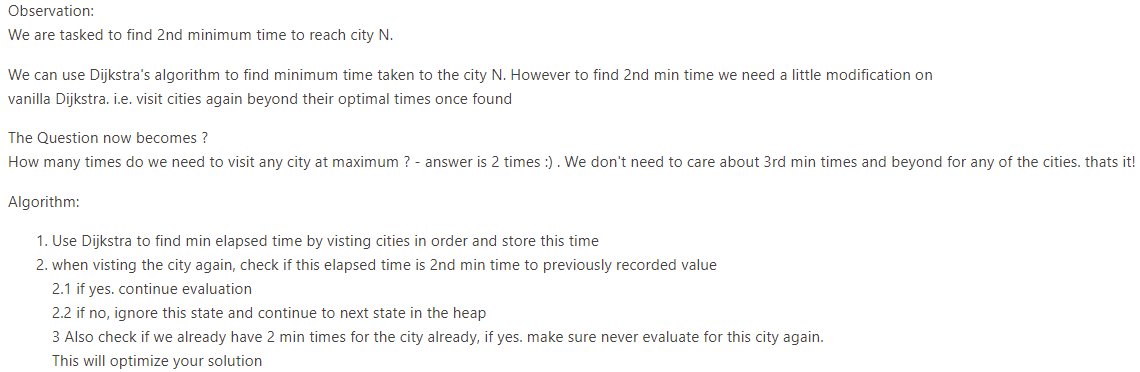
\includegraphics[width=.9\linewidth]{./pic/redGreen.png}

\begin{minted}[frame=lines,fontsize=\scriptsize,linenos=false]{java}
public int secondMinimum(int n, int[][] edges, int time, int change) {
    Map<Integer, List<Integer>> adj = new HashMap<>();
    for (int [] e : edges) {
        adj.computeIfAbsent(e[0], z -> new ArrayList<>()).add(e[1]);
        adj.computeIfAbsent(e[1], z -> new ArrayList<>()).add(e[0]);
    }
    Queue<int []> q = new PriorityQueue<>((a, b)->(a[1] -b[1]));
    q.offer(new int []{1, 0});
    Map<Integer, Integer> cache = new HashMap<>(); // use cache to record min time per city
    // modification: we want to visit each city maximum two times with different times,
    // this will help in early termination when we visit the city again (3rd time or more)
    Set<Integer> exhausted = new HashSet<>();
    while (!q.isEmpty()) {
        int [] top = q.poll();
        int cur = top[0], t = top[1];
        // Base Termination : we have found our 2nd min time for city n
        if (cur == n && t > cache.getOrDefault(cur, Integer.MAX_VALUE))
            return t;
        if (!cache.containsKey(cur)) // we vistied this city for first time, so elapsed time is min for this city
            cache.put(cur, t);
        // early termination, if we are trying to visit the city 3rd time or more ,
        // or the elapsed time will not help in finding the solution
        else if (cache.get(cur) == t || exhausted.contains(cur)) continue;
        else // this means we are visiting the city with 2nd optimal time , we dont need to visit the city ever again
            exhausted.add(cur);
        // we visit the city on elapsedTime, we need to check if on basis of change time, whether this time falls in  cycle (green or red)
        // if odd cycle (red), we must wait for this cycle to end
        int factor = t / change;
        if (factor % 2 == 1)
            t = (factor + 1) * change;
        for (int nb : adj.getOrDefault(cur, new ArrayList<>())) { // visit the neighbours
            int visTime = t + time;
            if (!exhausted.contains(nb))
                q.offer(new int [] {nb, visTime});
        }
    }
    return -1;
}
\end{minted}
\begin{itemize}
\item 另一个也是写得直接了当的
\end{itemize}
\begin{minted}[frame=lines,fontsize=\scriptsize,linenos=false]{java}
public int secondMinimum(int n, int [][] edges, int time, int change) {
    Map<Integer, Set<Integer>> map = new HashMap<>();
    for (int [] e : edges) {
        map.computeIfAbsent(e[0], z -> new HashSet<>()).add(e[1]);
        map.computeIfAbsent(e[1], z -> new HashSet<>()).add(e[0]);
    }
    Queue<int []> q = new PriorityQueue<>((a, b)->(a[1]-b[1]));
    Map<Integer, Set<Integer>> vis = new HashMap<>();
    q.offer(new int [] {1, 0});
    int min = -1;
    while (!q.isEmpty()) {
        int [] top = q.poll();
        int cur = top[0], t = top[1];
        if (cur == n) {
            if (min == -1 || min == t) min = t;
            else return t;
        }
        if (t % (2 * change) >= change)
            t += 2 * change - t % (2 * change);
        // 源码中传入key和value,根据key获取看是否存在value,如果value==null,然后调用put方法把传入的key和value  put进map,返回根据key获取的老value
        // 如果传入key对应的value已经存在,就返回存在的value,不进行替换。如果不存在,就添加key和value,返回null
        vis.putIfAbsent(cur, new HashSet<>());
        if (!vis.get(cur).add(t) || vis.get(cur).size() >= 3) continue;
        if (map.containsKey(cur))
            for (int next : map.get(cur)) 
                q.offer(new int [] {next, t + time});
    }
    return -1;
}
\end{minted}
昨天晚上的比赛,状态相对早上要差了很多,感觉到晚上的头脑已经不是很清醒。比赛的时候没有感觉,白白折腾了一个小时。
结束后去看别人题解的时候,弱弱的内心是奔溃的:
应该说这些考点平时自己也都练习过,没有过偏的地方,可为什么自己做题的时候,一个个考点穿上马甲我就再也认不出它们来了呢?
把可以重复遍历当作是多余的,不想去重复遍历;又被n迷惑住,全然忘记其它node也会被重复遍历到;明明知道pq里还有一堆杂物,比赛时却浑然想不到我是可以去裁枝优化的?!!!
昨天晚上的比赛应该是最近几周参加比赛以来做得相对较好的一次,可相比于早上最后一道题完全没有时间做、几乎没有下笔思路,这个最后一题留有整整一个小时,考点也都练习到过,却探肩而过、失之交臂、被自己活活折腾死。。。感触很多。。。。。。或许这也是一个磨砺心志、相定信念的过程吧?!!!练习练习练习、总结总结总结,让它们深入骨髓,一看便知似曾相识?

\section{1334. Floyd算法 - Find the City With the Smallest Number of Neighbors at a Threshold Distance - Medium}
\label{sec-18-2}
There are n cities numbered from 0 to n-1. Given the array edges where edges[i] = [fromi, toi, weighti] represents a bidirectional and weighted edge between cities fromi and toi, and given the integer distanceThreshold.

Return the city with the smallest number of cities that are reachable through some path and whose distance is at most distanceThreshold, If there are multiple such cities, return the city with the greatest number.

Notice that the distance of a path connecting cities i and j is equal to the sum of the edges' weights along that path.
\begin{minted}[frame=lines,fontsize=\scriptsize,linenos=false]{java}
public int findTheCity(int n, int[][] edges, int distanceThreshold) {
    // 1.创建邻接矩阵
    int [][] graph = new int [n][n]; // 相比于我只会用HashMap来建邻接关系,邻接链表与数组都可能,看哪个用起来方便
    for (int i = 0; i < n; i++)
        Arrays.fill(graph[i], Integer.MAX_VALUE); // pre filled n equaivlent to Integer.MAX_VALUE
    for (int [] eg : edges) {
        graph[eg[0]][eg[1]] = eg[2];
        graph[eg[1]][eg[0]] = eg[2];
    }
    // 2.floyd算法
    for (int k = 0; k < n; k++)          // 中间结点
        for (int i = 0; i < n; i++)      // 开始结点
            for (int j = 0; j < n; j++) {// 结尾结点
                if (i == j || graph[i][k] == Integer.MAX_VALUE || graph[k][j] == Integer.MAX_VALUE) continue;
                graph[i][j] = Math.min(graph[i][j], graph[i][k] + graph[k][j]);
            }                
    // 3.每个城市距离不大于distanceThreshold的邻居城市的数目
    int [] mark = new int [n]; //记录小于distanceThreshold的邻居城市个数
    for (int i = 0; i < n; i++) 
        for (int j = 0; j < n; j++) 
            if (graph[i][j] <= distanceThreshold)
                mark[i]++;
    // 4.找数目少,编号最大的
    int min = n;
    int ans = 0;
    for (int i = 0; i < n; i++) 
        if (min >= mark[i]) {
            min = mark[i];
            ans = i;
        }
    return ans;
}
\end{minted}
\begin{itemize}
\item 另一种解法
\end{itemize}
\begin{minted}[frame=lines,fontsize=\scriptsize,linenos=false]{java}
// 之前用原创想法也写了很多图的题,但缺乏归纳总结,原创想法更多的是解决了题目,但解法与效率、与优化算法间的距离还需要很多比较归纳与总结,才能把图这一块吃透
// https://leetcode.jp/leetcode-1334-find-the-city-with-the-smallest-number-of-neighbors-at-a-threshold-distance-%E8%A7%A3%E9%A2%98%E6%80%9D%E8%B7%AF%E5%88%86%E6%9E%90/  这个题需要重新写
// map:图结构
// city:当前城市
// dis:当前所剩距离
// v:已经被记录为邻居的节点
// maxDis:走到某个节点时,剩余距离的最大值
// 返回值为当前城市的邻居数。
private int dfs(int [][] arr, int city, int dis, boolean [] vis, int [] maxDis) {
    int res = 0;
    for (int i = 0; i < arr[0].length; i++) { // 循环当前城市的所有相邻城市
        int distance = arr[city][i]; // 与相邻城市的距离,如果为0,说明与该城市不相连
        int diffDis = dis - distance;// 到达相邻城市后,与阈值相比的剩余距离。
        if (distance > 0 && diffDis >= maxDis[i]) { // 与该城市相连并且剩余距离大于等于访问数组中的值
            maxDis[i] = diffDis;     // 更新访问数组中的剩余距离   
            if (!vis[i]) {
                vis[i] = true;
                res++;
            }
            res += dfs(arr, i, diffDis, vis, maxDis); // 递归dfs与该城市相连的其他城市:图中我似乎还很没有dfs以及递归的概念
        }
    }
    return res;
}
public int findTheCity(int n, int[][] edges, int distanceThreshold) {
    int [][] map = new int [n][n];
    for (int [] eg : edges) {
        map[eg[0]][eg[1]] = eg[2];
        map[eg[1]][eg[0]] = eg[2];
    }
    int min = n;
    int res = 0;
    for (int i = 0; i < n; i++) {
        boolean [] vis = new boolean [n];
        vis[i] = true;
        int cnt = dfs(map, i, distanceThreshold, vis, new int [n]);
        if (cnt <= min) {
            min = cnt;
            res = i;
        }
    }
    return res;
}
\end{minted}

\section{1129. Shortest Path with Alternating Colors - Medium}
\label{sec-18-3}
Consider a directed graph, with nodes labelled 0, 1, \ldots{}, n-1.  In this graph, each edge is either red or blue, and there could be self-edges or parallel edges.

Each [i, j] in red$_{\text{edges}}$ denotes a red directed edge from node i to node j.  Similarly, each [i, j] in blue$_{\text{edges}}$ denotes a blue directed edge from node i to node j.

Return an array answer of length n, where each answer[X] is the length of the shortest path from node 0 to node X such that the edge colors alternate along the path (or -1 if such a path doesn't exist).
\begin{minted}[frame=lines,fontsize=\scriptsize,linenos=false]{java}
// 找最短路径应该用queue来做,入队列的时候需要标记红边或是蓝边以便找交替路径
public int[] shortestAlternatingPaths(int n, int[][] red_edges, int[][] blue_edges) {
    HashMap<Integer, List<Integer>> [] maps = new HashMap [2]; // 0 : red; 1: blue
    for (int i = 0; i < 2; i++) 
        maps[i] = new HashMap<>();
    for (int i = 0; i < red_edges.length; i++) 
        maps[0].computeIfAbsent(red_edges[i][0], k->new ArrayList<>()).add(red_edges[i][1]);
    for (int i = 0; i < blue_edges.length; i++) 
        maps[1].computeIfAbsent(blue_edges[i][0], k->new ArrayList<>()).add(blue_edges[i][1]);
    int [] ans = new int[n];
    Arrays.fill(ans, -1);
    Queue<int []> q = new LinkedList<>();
    q.offer(new int [] {0, 0}); // red edge         
    q.offer(new int [] {0, 1}); // blue edge
    boolean [][] inQueue = new boolean [n][2]; // 0: red, 1: blue
    inQueue[0][0] = true;
    inQueue[0][1] = true;
    int cnt = 0, color = 0;
    while (!q.isEmpty()) {
        for (int size = q.size(); size > 0; size--) {
            int [] cur = q.poll();
            System.out.println(Arrays.toString(cur));
            color = cur[1];
            if (ans[cur[0]] == -1) ans[cur[0]] = cnt;
            List<Integer> nextNodes = maps[1-color].get(cur[0]);
            if (nextNodes == null) continue;
            for (Integer next : nextNodes) 
                if (!inQueue[next][1-color]) {
                    q.offer(new int [] {next, 1-color});
                    inQueue[next][1-color] = true;
                }
        }
        ++cnt;
    }
    return ans;
}
\end{minted}
\begin{itemize}
\item 不是总喜欢省掉大括号吗,试试省掉下面的。。。。。。
\end{itemize}
\begin{minted}[frame=lines,fontsize=\scriptsize,linenos=false]{java}
public int[] shortestAlternatingPaths(int n, int[][] red_edges, int[][] blue_edges) {
    int [][] red = new int[n][2]; // 红 0 蓝 1
    int [][] blue = new int[n][2];
    for (int i = 1; i < n; i++) {
        red[i][0] = i;
        red[i][1] = 0x0fffffff;   // 初始化红边权值
    }
    red [0][0] = 0;
    red [0][1] = 0;
    for (int i = 1; i < n; i++) {
        blue[i][0] = i;
        blue[i][1] = 0x0fffffff;
    }
    blue [0][0] = 0;
    blue [0][1] = 0;
    dfs(red, blue, 0, 0, red_edges, blue_edges);
    dfs(red, blue, 1, 0, red_edges, blue_edges);
    int [] ans = new int[n];
    for(int i = 0; i < n; i++){
        ans[i] = Math.min(red[i][1], blue[i][1]);
        if (ans[i] == 0x0fffffff) // 没有改变说明不存在
            ans[i] = -1;
    }
    return ans;
}
public void dfs(int [][] red, int [][] blue, int color, int node, int[][] red_edges, int[][] blue_edges){
    if (color == 0) { // 这个括号可以省吗???
        for (int [] blue_to : blue_edges) // 以node为from to 为终 的边
            if (node == blue_to[0] && red[node][1]+1 < blue[blue_to[1]][1]) {// 0到from点加1是否小于0到to的距离
                blue[blue_to[1]][1] = red[node][1]+1; // 作距离的更新
                dfs(red, blue, 1-color, blue_to[1], red_edges, blue_edges);
            }
    } else for (int [] red_to : red_edges) //以node为from to 为终 的边
               if (node == red_to[0] && blue[node][1]+1 < red[red_to[1]][1]) {//0到from点加1是否小于0到to的距离
                   red[red_to[1]][1] = blue[node][1]+1;
                   dfs(red, blue, 1-color, red_to[1], red_edges, blue_edges);
               }
}
\end{minted}

\section{882. Reachable Nodes In Subdivided Graph - Hard}
\label{sec-18-4}
You are given an undirected graph (the "original graph") with n nodes labeled from 0 to n - 1. You decide to subdivide each edge in the graph into a chain of nodes, with the number of new nodes varying between each edge.

The graph is given as a 2D array of edges where edges[i] = [ui, vi, cnti] indicates that there is an edge between nodes ui and vi in the original graph, and cnti is the total number of new nodes that you will subdivide the edge into. Note that cnti == 0 means you will not subdivide the edge.

To subdivide the edge [ui, vi], replace it with (cnti + 1) new edges and cnti new nodes. The new nodes are x1, x2, \ldots{}, xcnti, and the new edges are [ui, x1], [x1, x2], [x2, x3], \ldots{}, [xcnti-1, xcnti], [xcnti, vi].

In this new graph, you want to know how many nodes are reachable from the node 0, where a node is reachable if the distance is maxMoves or less.

Given the original graph and maxMoves, return the number of nodes that are reachable from node 0 in the new graph.

再进一步来分析,其实上对于每个结点来说(不论有没有编号),若我们能算出该结点离起始结点的最短距离,且该距离小于等于M的话,那这个结点就一定可以到达。这样来说,其实本质就是求单源点的最短距离,此时就要祭出神器迪杰斯特拉算法 Dijkstra Algorithm 了,LeetCode 中使用了该算法的题目还有 Network Delay Time 和 The Maze II。该算法的一般形式是用一个最小堆来保存到源点的最小距离,这里我们直接统计到源点的最小距离不是很方便,可以使用一个小 trick,即用一个最大堆来统计当前结点所剩的最大步数,因为剩的步数越多,说明距离源点距离越小。由于 Dijkstra 算法是以起点为中心,向外层层扩展,直到扩展到终点为止。根据这特性,用 BFS 来实现时再好不过了,首先来建立邻接链表,这里可以使用一个 NxN 的二维数组 graph,其中 graph[i][j] 表示从大结点i往大结点j方向会经过的小结点个数,建立邻接链表的时候对于每个 edge,要把两个方向都赋值,前面解释过了这里要当作有向图来做。然后使用一个最大堆,里面放剩余步数和结点编号组成的数对儿,把剩余步数放前面就可以默认按步数从大到小排序了,初始化时把 \{M,0\} 存入最大堆。还需要一个一维数组 visited 来记录某个结点是否访问过。

\begin{minted}[frame=lines,fontsize=\scriptsize,linenos=false]{java}
public int reachableNodes(int[][] edges, int maxMoves, int n) {
    int [][] graph = new int  [n][n];
    for (int i = 0; i < n; i++) 
        Arrays.fill(graph[i], -1);
    for (int [] v : edges) {
        graph[v[0]][v[1]] = v[2];
        graph[v[1]][v[0]] = v[2];
    }
    Queue<int []> q = new PriorityQueue<>((a, b) -> (b[0] - a[0]));
    boolean [] vis = new boolean [n];
    q.offer(new int [] {maxMoves, 0});
    int res = 0;
    while (!q.isEmpty()) {
        int [] cur = q.poll();
        int cnt = cur[0], u = cur[1];
        if (vis[u]) continue;
        vis[u] = true;
        ++res;
        for (int i = 0; i < n; i++) {
            if (graph[u][i] == -1) continue;
            if (cnt > graph[u][i] && !vis[i])
                q.offer(new int [] {cnt - graph[u][i]-1, i});
            graph[i][u] -= Math.min(cnt, graph[u][i]);
            res += Math.min(cnt, graph[u][i]);
        }
    }
    return res;
}
\end{minted}
\begin{itemize}
\item 我们也可以使用 HashMap 来建立邻接链表,最后的运行速度果然要比二维数组形式的邻接链表要快一些,其他的地方都不变,参见代码如下:
\end{itemize}
\begin{minted}[frame=lines,fontsize=\scriptsize,linenos=false]{java}
public int reachableNodes(int[][] edges, int maxMoves, int n) {
    int res = 0;
    Map<Integer, Map<Integer, Integer>> graph = new HashMap<>();
    for (int [] v : edges) {
        graph.computeIfAbsent(v[0], k->new HashMap<>()).put(v[1], v[2]);
        graph.computeIfAbsent(v[1], k->new HashMap<>()).put(v[0], v[2]);
    }
    Queue<int []> q = new PriorityQueue<>((a, b) -> (b[0] - a[0]));
    boolean [] vis = new boolean [n];
    q.offer(new int [] {maxMoves, 0});
    while (!q.isEmpty()) {
        int [] cur = q.poll();
        int cnt = cur[0], u = cur[1];
        if (vis[u]) continue;
        vis[u] = true;
        ++res;
        for (int i = 0; i < n; i++) {
            if (!graph.containsKey(u) || !graph.get(u).containsKey(i) || graph.get(u).get(i) == -1) continue;
            if (cnt > graph.get(u).get(i) && !vis[i])
                q.offer(new int [] {cnt - graph.get(u).get(i)-1, i});
            graph.get(i).put(u, graph.get(u).get(i) - Math.min(cnt, graph.get(u).get(i)));
            res += Math.min(cnt, graph.get(u).get(i));
        }
    }
    return res;
}
\end{minted}

\section{1782. Count Pairs Of Nodes - Hard}
\label{sec-18-5}
You are given an undirected graph defined by an integer n, the number of nodes, and a 2D integer array edges, the edges in the graph, where edges[i] = [ui, vi] indicates that there is an undirected edge between ui and vi. You are also given an integer array queries.

Let incident(a, b) be defined as the number of edges that are connected to either node a or b.

The answer to the jth query is the number of pairs of nodes (a, b) that satisfy both of the following conditions:

a < b
incident(a, b) > queries[j]
Return an array answers such that answers.length == queries.length and answers[j] is the answer of the jth query.

Note that there can be multiple edges between the same two nodes.
\begin{minted}[frame=lines,fontsize=\scriptsize,linenos=false]{java}
// https://leetcode.com/problems/count-pairs-of-nodes/discuss/1096740/C%2B%2BJavaPython3-Two-Problems-O(q-*-(n-%2B-e))
public int[] countPairs(int n, int[][] edges, int[] queries) { // 别人家的思路好清晰
    int [] cnt = new int [n+1], sortedCnt = new int [n+1], ans = new int [queries.length];
    Map<Integer, Integer> [] m = new HashMap[n+1];
    for (var e : edges) {
        sortedCnt[e[0]] = cnt[e[0]] = cnt[e[0]] + 1;
        sortedCnt[e[1]] = cnt[e[1]] = cnt[e[1]] + 1;
        int min = Math.min(e[0], e[1]), max = Math.max(e[0], e[1]);
        m[min] = m[min] == null ? new HashMap<>() : m[min];
        m[min].put(max, m[min].getOrDefault(max, 0) + 1); // 仍然是当作有向图、单向图来做
    }
    Arrays.sort(sortedCnt);
    int res = 0, cur = 0;
    for (int k = 0; k < queries.length; k++) {
        for (int i = 1, j = n; i < j;) 
            if (queries[k] < sortedCnt[i] + sortedCnt[j])
                ans[k] += (j--) - i;
            else ++i;
        for (int i = 1; i <= n; i++) 
            if (m[i] != null) 
                for (var en : m[i].entrySet()) {
                    int j = en.getKey(), sharedCnt = en.getValue();
                    if (queries[k] < cnt[i] + cnt[j] && cnt[i] + cnt[j] - sharedCnt <= queries[k])
                        ans[k]--;
                }
    } 
    return ans;
}
\end{minted}

\section{332. Reconstruct Itinerary - Medium}
\label{sec-18-6}
You are given a list of airline tickets where tickets[i] = [fromi, toi] represent the departure and the arrival airports of one flight. Reconstruct the itinerary in order and return it.

All of the tickets belong to a man who departs from "JFK", thus, the itinerary must begin with "JFK". If there are multiple valid itineraries, you should return the itinerary that has the smallest lexical order when read as a single string.

For example, the itinerary ["JFK", "LGA"] has a smaller lexical order than ["JFK", "LGB"].
You may assume all tickets form at least one valid itinerary. You must use all the tickets once and only once.
\begin{minted}[frame=lines,fontsize=\scriptsize,linenos=false]{java}
private void dfs(String cur, List<String> list) {
    Queue<String> next = m.get(cur);
    while (next != null && next.size() > 0) 
        dfs(next.poll(), list);
    list.add(cur);
}
Map<String, PriorityQueue<String>> m = new HashMap<>();      // TreeSet does not handle repeats, use queue
public List<String> findItinerary(List<List<String>> tickets) {
    for (int i = 0; i < tickets.size(); i++) 
        m.computeIfAbsent(tickets.get(i).get(0), k -> new PriorityQueue<>()).offer(tickets.get(i).get(1));
    List<String> res = new ArrayList<>();
    dfs("JFK", res);
    Collections.reverse(res);
    return res;
}
\end{minted}

\section{1591. Strange Printer II - Hard}
\label{sec-18-7}
There is a strange printer with the following two special requirements:

On each turn, the printer will print a solid rectangular pattern of a single color on the grid. This will cover up the existing colors in the rectangle.
Once the printer has used a color for the above operation, the same color cannot be used again.
You are given a m x n matrix targetGrid, where targetGrid[row][col] is the color in the position (row, col) of the grid.

Return true if it is possible to print the matrix targetGrid, otherwise, return false.

这道题可以认为是在研究:是否有一种颜色序列,按照这个序列进行染色,最终矩阵就会呈现输入的状态。

矩形上的某一个像素点,可能会先后经历多次染色。比如先染红,再染绿,再染黄,最后染蓝,最后呈现出的就是蓝色。

我们知道这个像素现在是蓝色;

而它在红色/绿色/黄色矩形范围内,说明这个像素曾经红过/绿过/黄过。

此时我们可以提炼出信息:假定先染的优先于后染的,那么红色优于蓝色,绿色优于蓝色,黄色优于蓝色。

(红绿黄之间的顺序未定)。

题中指出,颜色最多有 6060 种,我们可以建立一个有向图,图中的结点就是这 6060 个颜色 1$\sim$ 601∼60 。

按照刚才的方法找出所有的有向边,进行拓扑排序即可判断出结果。

\begin{minted}[frame=lines,fontsize=\scriptsize,linenos=false]{java}
public boolean isPrintable(int[][] targetGrid) { // 觉得这个题思路奇特
    int m = targetGrid.length, n = targetGrid[0].length, max = Math.max(m, n);
    for (int i = 0; i < m; i++) 
        max = Math.max(max, Arrays.stream(targetGrid[i]).max().getAsInt());
    int [] top = new int [max+1], bot = new int [max+1], left = new int [max+1], right = new int [max+1];
    Arrays.fill(top, max+1);
    Arrays.fill(left, max+1);
    Arrays.fill(bot, -1);
    Arrays.fill(right, -1);
    for (int i = 0; i < m; i++) // 建立每个颜色的矩阵边界: 界定每种颜色的上下左右边界,每种颜色最早(上左)最晚(下右)出现的位置
        for (int j = 0; j < n; j++) {
            int color = targetGrid[i][j];
            top[color] = Math.min(top[color], i);
            bot[color] = Math.max(bot[color], i);
            left[color] = Math.min(left[color], j);
            right[color] = Math.max(right[color], j);
        }
    // 根据矩阵建立有向图,遍历targetGrid,
    // 当前位置颜色X在某个矩阵A中但是不为矩阵A的颜色时,建立从A到X的边
    // X可以存在于多个矩阵中
    // 变量:是否存在边-防止重复建立边;入度,便于后期判断是否拓扑排序;邻接表,从i出发到达的点
    boolean [][] eg = new boolean [max+1][max+1];
    int [] ins = new int [max+1];
    List<List<Integer>> adj = new ArrayList<>();
    for (int i = 0; i <= max; i++) 
        adj.add(new ArrayList<>());
    int cur = 0; // 建立图
    for (int i = 0; i < m; i++) 
        for (int j = 0; j < n; j++) {
            cur = targetGrid[i][j]; // 当前格子的最终打印顔色
            for (int color = 1; color <= max; color++) // 遍历所有颜色:暴搜当前格子颜色是否可能后打印
                if (i >= top[color] && i <= bot[color] && j >= left[color] && j <= right[color])
                    if (cur != color && !eg[color][cur]) {
                        adj.get(color).add(cur); // color 先染后,cur后染色
                        ins[cur]++;
                        eg[color][cur] = true;
                    }
        }
    // 寻找入度为0的颜色点,减小该点连结的点的入度,直到所有点的入度都为0
    List<Integer> l = new ArrayList<>();
    while (true) {
        int i;
        for (i = 1; i <= max; i++) 
            if (ins[i] == 0) {
                l.add(i);
                for (int v : adj.get(i)) ins[v]--;
                ins[i] = -1;
                break;
            }
        if (i == max+1) break;
    }
    return l.size() == max;
}
\end{minted}
\begin{itemize}
\item topological sort
\end{itemize}
\begin{minted}[frame=lines,fontsize=\scriptsize,linenos=false]{java}
private boolean topologicalSort(Set<Integer> visited, Set<Integer> visiting, int c, Map<Integer, Set<Integer>> graph) {
    if (visited.contains(c)) return true;
    if (visiting.contains(c)) return false;
    visiting.add(c);
    for (Integer nei : graph.getOrDefault(c, Collections.emptySet())) 
        if (!topologicalSort(visited, visiting, nei, graph)) return  false;
    visiting.remove(c);
    visited.add(c);
    return true;
}
// 1. For each color, find left top corner and right bottom corner
// 2. All colors interfering with given color means they should go after given
// 3. Create dependencies (1 -> [2,3])
// 4. TopSort. Loops mean it is not possible
public boolean isPrintable(int[][] targetGrid) {
    Map<Integer, Set<Integer>> graph = new HashMap<>();
    Set<Integer> colors = new HashSet<>();
    int m = targetGrid.length, n = targetGrid[0].length;
    for (int i = 0; i < m; i++) 
        for (int j = 0; j < n; j++) 
            colors.add(targetGrid[i][j]);
    for (Integer c : colors) {
        int fi = -1, fj = Integer.MAX_VALUE, li = -1, lj = -1; // f: first, f row, f col, l: last, l row, l col
        for (int i = 0; i < m; i++) 
            for (int j = 0; j < n; j++) 
                if (targetGrid[i][j] == c) {
                    if (fi == -1) fi = i;
                    fj = Math.min(fj, j);
                    li = i;
                    lj = Math.max(lj, j);
                }
        for (int i = fi; i <= li; i++) 
            for (int j = fj; j <= lj; j++) 
                if (targetGrid[i][j] != c) 
                    graph.computeIfAbsent(c, z -> new HashSet<>()).add(targetGrid[i][j]);
    }
    Set<Integer> visited = new HashSet<>();
    Set<Integer> visiting = new HashSet<>();
    for (Integer c : colors) 
        if (!topologicalSort(visited, visiting, c, graph)) return false;
    return true;
}
\end{minted}

\chapter{扫描线}
\label{sec-19}
\section{218. The Skyline Problem - Hard}
\label{sec-19-1}
A city's skyline is the outer contour of the silhouette formed by all the buildings in that city when viewed from a distance. Given the locations and heights of all the buildings, return the skyline formed by these buildings collectively.

The geometric information of each building is given in the array buildings where buildings[i] = [lefti, righti, heighti]:

lefti is the x coordinate of the left edge of the ith building.
righti is the x coordinate of the right edge of the ith building.
heighti is the height of the ith building.
You may assume all buildings are perfect rectangles grounded on an absolutely flat surface at height 0.

The skyline should be represented as a list of "key points" sorted by their x-coordinate in the form [[x1,y1],[x2,y2],\ldots{}]. Each key point is the left endpoint of some horizontal segment in the skyline except the last point in the list, which always has a y-coordinate 0 and is used to mark the skyline's termination where the rightmost building ends. Any ground between the leftmost and rightmost buildings should be part of the skyline's contour.

Note: There must be no consecutive horizontal lines of equal height in the output skyline. For instance, [\ldots{},[2 3],[4 5],[7 5],[11 5],[12 7],\ldots{}] is not acceptable; the three lines of height 5 should be merged into one in the final output as such: [\ldots{},[2 3],[4 5],[12 7],\ldots{}]

使用扫描线,从左至右扫过。如果遇到左端点,将高度入堆,如果遇到右端点,则将高度从堆中删除。使用 last 变量记录上一个转折点。

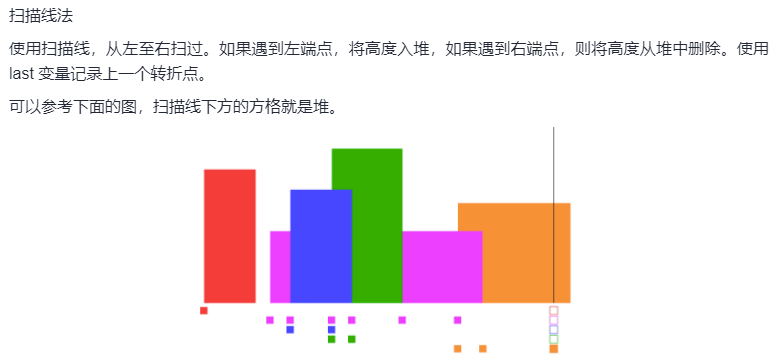
\includegraphics[width=.9\linewidth]{./pic/sweep.png}

\begin{minted}[frame=lines,fontsize=\scriptsize,linenos=false]{java}
public List<List<Integer>> getSkyline(int[][] buildings) { // 从左向右扫一遍过去
    List<List<Integer>> ans = new ArrayList<>();
    Map<Integer, List<Integer>> map = new TreeMap<>();
    for (int [] v : buildings) {
        map.computeIfAbsent(v[0], z -> new ArrayList<>()).add(-v[2]); // 插入左节点: 高度为负
        map.computeIfAbsent(v[1], z -> new ArrayList<>()).add(v[2]);  // 插入右节点:高度为正
    }
    Map<Integer, Integer> heights = new TreeMap<>((a, b) -> b-a); // 保留当前位置的所有高度 重定义排序:从大到小
    int [] last = {0, 0}; // 保留上一个位置的横坐标及高度           
    for (Integer key : map.keySet()) {
        List<Integer> ys = map.get(key);
        Collections.sort(ys);
        for (int y : ys) {
            if (y < 0) // 左端点,高度入队
                heights.put(-y, heights.getOrDefault(-y, 0) + 1);
            else {     // 右端点移除高度
                heights.put(y, heights.getOrDefault(y, 1) - 1);
                if (heights.get(y) == 0) heights.remove(y);
            }
        }
        Integer maxHeight = 0;      // 获取heights的最大值:就是第一个值
        if (!heights.isEmpty())
            maxHeight = heights.keySet().iterator().next();
        if (last[1] != maxHeight) { // 如果当前最大高度不同于上一个高度,说明其为转折点
            last[0] = key;          // 更新last,并加入结果集
            last[1] = maxHeight;
            ans.add(Arrays.asList(key, maxHeight));
        }
    }
    return ans;
}
\end{minted}

\section{715. Range Module - Hard}
\label{sec-19-2}
A Range Module is a module that tracks ranges of numbers. Design a data structure to track the ranges represented as half-open intervals and query about them.

A half-open interval [left, right) denotes all the real numbers x where left <= x < right.

Implement the RangeModule class:

RangeModule() Initializes the object of the data structure.
void addRange(int left, int right) Adds the half-open interval [left, right), tracking every real number in that interval. Adding an interval that partially overlaps with currently tracked numbers should add any numbers in the interval [left, right) that are not already tracked.
boolean queryRange(int left, int right) Returns true if every real number in the interval [left, right) is currently being tracked, and false otherwise.
void removeRange(int left, int right) Stops tracking every real number currently being tracked in the half-open interval [left, right).
\begin{minted}[frame=lines,fontsize=\scriptsize,linenos=false]{java}
    class Range {
        int left, right;
        public Range(int left, int right) {
            this.left = left;
            this.right = right;
        }
    }
    TreeSet<Range> ts;
    public RangeModule() {
        ts = new TreeSet<>((a, b)->(a.left != b.left ? a.left - b.left : a.right - b.right));
    }
    public void addRange(int left, int right) {
        int nl = left, nr = right;
        Range high = new Range(right, Integer.MAX_VALUE);
        while (true) {
            Range r = ts.lower(high);
            if (r == null || r.right < left) break;
            if (r.right > right) nr = r.right;
            if (r.left < left) nl = r.left;
            ts.remove(r);
        }
        ts.add(new Range(nl, nr));
    }
    public boolean queryRange(int left, int right) {
        Range target = ts.floor(new Range(left, Integer.MAX_VALUE));
        return target != null && target.left <= left && target.right >= right;
    }
    public void removeRange(int left, int right) {
        Range high = new Range(right, right);
        while (true) {
            Range r = ts.lower(high);
            if (r == null || r.right <= left) break;
            if (r.right > right)
                ts.add(new Range(right, r.right));
            if (r.left < left)
                ts.add(new Range(r.left, left));
            ts.remove(r);
        }
    }
\end{minted}

\section{352. Data Stream as Disjoint Intervals - Hard}
\label{sec-19-3}
Given a data stream input of non-negative integers a1, a2, \ldots{}, an, summarize the numbers seen so far as a list of disjoint intervals.

Implement the SummaryRanges class:

SummaryRanges() Initializes the object with an empty stream.
void addNum(int val) Adds the integer val to the stream.
int[][] getIntervals() Returns a summary of the integers in the stream currently as a list of disjoint intervals [starti, endi].
\begin{minted}[frame=lines,fontsize=\scriptsize,linenos=false]{java}
    class Range implements Comparable<Range> {
        int bgn, end;
        public Range(int bgn, int end) {
            this.bgn = bgn;
            this.end = end;
        }
        @Override public int compareTo(Range other) {
            return this.bgn - other.bgn;
        }
    }
    TreeSet<Range> ts; 
    public SummaryRanges() {
        ts = new TreeSet<Range>();
    }
    public void addNum(int val) {
        Range cur = new Range(val, val);
        Range bef = ts.floor(cur);
        Range aft = ts.ceiling(cur);
        if (bef != null && bef.end + 1 >= val) {
            cur.bgn = bef.bgn;
            cur.end = Math.max(val, bef.end);
            ts.remove(bef);
        }
        if (aft != null && aft.bgn == val + 1) {
            cur.end = aft.end;
            ts.remove(aft);
        }
        ts.add(cur);
    }
    public int[][] getIntervals() {
        int [][] ans = new int [ts.size()][2];
        int i = 0;
        for (Range cur : ts) {
            ans[i][0] = cur.bgn;
            ans[i][1] = cur.end;
            i++;
        }
        return ans;
    }
\end{minted}

\section{1419. Minimum Number of Frogs Croaking - Medium}
\label{sec-19-4}
Given the string croakOfFrogs, which represents a combination of the string "croak" from different frogs, that is, multiple frogs can croak at the same time, so multiple “croak” are mixed. Return the minimum number of different frogs to finish all the croak in the given string.

A valid "croak" means a frog is printing 5 letters ‘c’, ’r’, ’o’, ’a’, ’k’ sequentially. The frogs have to print all five letters to finish a croak. If the given string is not a combination of valid "croak" return -1.
\begin{minted}[frame=lines,fontsize=\scriptsize,linenos=false]{java}
public int minNumberOfFrogs(String s) { // 写得有点儿乱
    int n = s.length();
    int cc = 0, cr = 0, co = 0, ca = 0, cnt = 0, max = 0;
    for (int i = 0; i < n; i++) {
        char c = s.charAt(i);
        if (c == 'c') {
            ++cc;
            ++cnt;
            max = Math.max(max, cnt);
        } else if (c == 'r') {
            if (cc == 0) return -1;
            --cc;
            ++cr;
        } else if (c == 'o') {
            if (cr == 0) return -1;
            --cr;
            ++co;
        } else if (c == 'a') {
            if (co == 0) return -1;
            --co;
            ++ca;
        } else if (c == 'k') {
            if (ca == 0) return -1;
            --ca;
            --cnt;
        }
    }
    if (cc + cr + co + ca > 0) return -1;
    return max;
}
\end{minted}

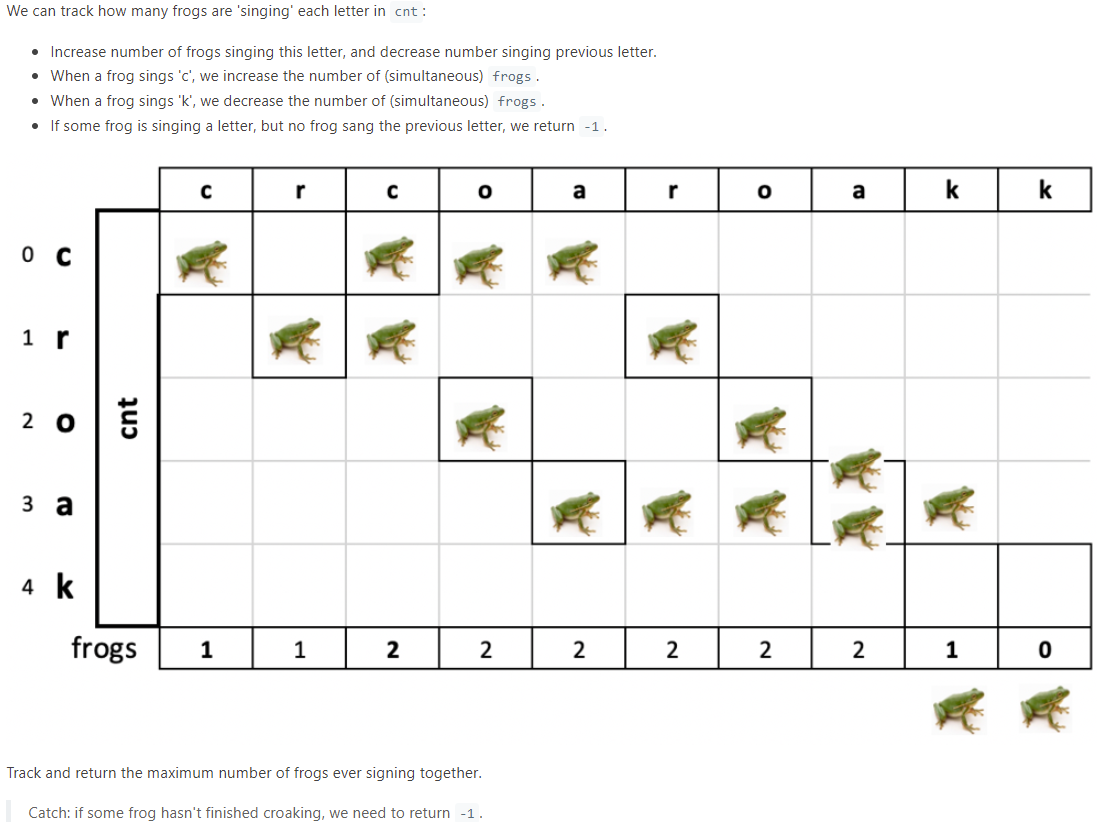
\includegraphics[width=.9\linewidth]{./pic/frogs.png}
\begin{minted}[frame=lines,fontsize=\scriptsize,linenos=false]{java}
public int minNumberOfFrogs(String s) {
    int n = s.length();
    int cnt [] = new int [5];
    int cur = 0, max = 0;
    for (int i = 0; i < n; i++) {
        char c = s.charAt(i);
        int idx = "croak".indexOf(c);
        ++cnt[idx];
        if (idx == 0)
            max = Math.max(max, ++cur);
        else if (--cnt[idx-1] < 0)
            return -1;
        else if (idx == 4)
            --cur;
    }
    return cur == 0 ? max : -1; // 如果最后所有的青蛙都叫完了的话  
}
\end{minted}
\begin{itemize}
\item 解法三:
\end{itemize}

这个跟上面的解法差不多,优化了查询位置的时间。直接对比每一步的结果。如果当前字符位的个数比上一位多,那么说明当前位没有办法被匹配成功。

\begin{minted}[frame=lines,fontsize=\scriptsize,linenos=false]{java}
public int minNumberOfFrogs(String croakOfFrogs) {
    char[] ch = croakOfFrogs.toCharArray();
    int curr = 0;
    int res = 0;
    int c = 0, r = 0, o = 0, a = 0, k = 0;
    for(int i = 0; i < ch.length; i++) {
        if(ch[i] == 'c') {
            c++;
            curr++;
        } else if(ch[i] == 'r') 
            r++;
        else if(ch[i] == 'o') 
            o++;
         else if(ch[i] == 'a') 
            a++;
         else {
            k++; 
            curr--;
        }
        res = Math.max(res, curr);
        if (c < r || r < o || o < a || a < k) // 要满足所有的条件
            return -1;
    }
    if ((c == r) && (r == o ) && ( o == a) &&  (a == k)) 
        return res;
    return -1;
}
\end{minted}


\chapter{PreSum}
\label{sec-20}
\section{1074. Number of Submatrices That Sum to Target - Hard 二维数组转化为一维数组:  数组中target Sum的2D版、presum思想的2d版}
\label{sec-20-1}
Given a matrix and a target, return the number of non-empty submatrices that sum to target.

A submatrix x1, y1, x2, y2 is the set of all cells matrix[x][y] with x1 <= x <= x2 and y1 <= y <= y2.

Two submatrices (x1, y1, x2, y2) and (x1', y1', x2', y2') are different if they have some coordinate that is different: for example, if x1 != x1'.

本题也需要使用到presum思路来解题,只不过这个前缀和presum的计算对象是二维数组。对于任意一个点,presum[i][j]代表了从Matrix\footnotemark[2]{}\textsuperscript{,}\,\footnotemark[2]{}到Matrix[i][j]之间的和。

有了前缀和之后,我们可以将二维数组拆解为多个一维数组,再用一维数组的思路去解题。

拆分数组时可以以列拆分,也可以以行拆,无论如何都可以达到遍历所有子矩阵的效果。本题以列拆分为例,对于任意两列col1和col2,我们可以得到所有行的前缀和

这样,二维数组就转化为了一维数组。接下来只要遍历所有列的组合即可。
\begin{minted}[frame=lines,fontsize=\scriptsize,linenos=false]{java}
public int numSubmatrixSumTarget(int[][] matrix, int target) {
    int m = matrix.length, n = matrix[0].length, rowSum = 0;
    int [][] sum = new int [m][n]; // sums of row sum only
    for (int i = 0; i < m; i++) {
        rowSum = 0;
        for (int j = 0; j < n; j++) {
            rowSum += matrix[i][j];
            sum[i][j] = rowSum + (i == 0 ? 0 : sum[i-1][j]);
        }
    }
    int cnt = 0, cur = 0;
    for (int j = 0; j < n; j++)     // col1
        for (int k = j; k < n; k++) {// col2
            Map<Integer, Integer> map = new HashMap<>(); // 用于记录前缀和个数
            for (int i = 0; i < m; i++) {
                cur = sum[i][k] - (j == 0 ? 0 : sum[i][j-1]);
                if (cur == target) ++cnt;
                cnt += map.getOrDefault(cur - target, 0);
                map.put(cur, map.getOrDefault(cur, 0) + 1);
            }
        }
    return cnt;
}
\end{minted}
\begin{itemize}
\item 对corner case的处理相对简洁的写法
\end{itemize}
\begin{minted}[frame=lines,fontsize=\scriptsize,linenos=false]{java}
public int numSubmatrixSumTarget(int [][] matrix, int target) { 
    int res = 0, m = matrix.length, n = matrix[0].length;
    int [][] sum = new int [m+1][n+1];
    for (int i = 1; i <= m; ++i) 
        for (int j = 1; j <= n; ++j) // 对全数组纵横求和
            sum[i][j] = sum[i][j - 1] + sum[i - 1][j] - sum[i - 1][j - 1] + matrix[i - 1][j - 1];
    for (int i = 1; i <= m; ++i) 
        for (int j = 1; j <= n; ++j) 
            for (int p = 1; p <= i; ++p) 
                for (int q = 1; q <= j; ++q) {
                    int t = sum[i][j] - sum[i][q - 1] - sum[p - 1][j] + sum[p - 1][q - 1];
                    if (t == target) ++res;
                }
    return res;
}
\end{minted}
\begin{minted}[frame=lines,fontsize=\scriptsize,linenos=false]{java}
public int numSubmatrixSumTarget(int[][] matrix, int target) {
    int m = matrix.length, n = matrix[0].length;
    int [][] sum = new int [m][n+1];                // sums of row sum only
    for (int i = 0; i < m; i++) {
        for (int j = 0; j < n; j++) 
            sum[i][j+1] = sum[i][j] + matrix[i][j]; // row sums only
    }
    int cnt = 0, cur = 0;
    for (int j = 0; j < n; j++)      // col1
        for (int k = j; k < n; k++) {// col2
            cur = 0;
            Map<Integer, Integer> map = new HashMap<>(); // 用于记录前缀和个数
            map.put(0, 1);
            for (int i = 0; i < m; i++) {
                cur += sum[i][k+1] - sum[i][j];
                cnt += map.getOrDefault(cur - target, 0);
                map.put(cur, map.getOrDefault(cur, 0) + 1);
            }
        }
    return cnt;
}
\end{minted}
解题思路分析

首先对每一行,计算一个presum

然后对任意两个列, [j,k], 计算j和k之间的所有数的和, 因为对于每一行,我们已经计算了presum, 所以,

对于[j,k]之间的树,可以通过presum[i][k] - (j == 0 ? 0 : presum[i][j-1])得到某一行在[j,k]之间的值

这样, 对于任意两列[j,k]之间的数, 我们可以形成一个临时的一维数组, 表示从第0行到最后一行的数,

那么, 问题就转换成在这个一维数组里面,找一个连续子数组, 使得这些数的和是target,

那么,后面这个问题就转换成 leetcode 560

\url{http://www.noteanddata.com/leetcode-560-Subarray-Sum-Equals-K-java-solution-note.html}

所以, 这个是presum思想的2d版, 类似的题目还有leetcode 304 Range Sum Query 2D - Immutable
\begin{minted}[frame=lines,fontsize=\scriptsize,linenos=false]{java}
public int numSubmatrixSumTarget(int [][] matrix, int target) {
    int res = 0, m = matrix.length, n = matrix[0].length;
    for (int i = 0; i < m; ++i) 
        for (int j = 1; j < n; ++j) 
            matrix[i][j] += matrix[i][j - 1];
    for (int i = 0; i < n; ++i) 
        for (int j = i; j < n; ++j) {
            Map<Integer, Integer> cntMap = new HashMap<>();
            cntMap.put(0, 1);
            int cur = 0;
            for (int k = 0; k < m; ++k) {
                cur += matrix[k][j] - (i > 0 ? matrix[k][i - 1] : 0);
                res += cntMap.getOrDefault(cur-target, 0);
                cntMap.put(cur, cntMap.getOrDefault(cur, 0) + 1);
            }
        }
    return res;
}
\end{minted}
\begin{minted}[frame=lines,fontsize=\scriptsize,linenos=false]{java}
private int cntTarget(int [] arr, int target) { // 比较一下与上面解法、写法的不同!!!
    int cnt = 0, sum = 0;
    Map<Integer, Integer> cntMap = new HashMap<>();
    cntMap.put(0, 1);
    for (int i = 0; i < arr.length; i++) {
        sum += arr[i];
        cnt += cntMap.getOrDefault(sum - target, 0);
        cntMap.compute(sum, (k, v) -> { // 
                if (v == null) v = 0;
                return v+1;
            });
        return cnt;
    }
}
public int numSubmatrixSumTarget(int[][] matrix, int target) {
    int m = matrix.length, n = matrix[0].length, cur = 0;
    int [][] sum = new int [m][n]; // sums of row sum only
    for (int i = 0; i < m; i++) {
        cur = 0;
        for (int j = 0; j < n; j++) {
            cur += matrix[i][j];
            sum[i][j] = cur;
        }
    }
    int cnt = 0;
    for (int j = 0; j < n; j++) {
        for (int k = j; k < n; k++) {
            int [] tmp = new int [m];
            for (int i = 0; i < m; i++) 
                tmp[i] = sum[i][k] - (j == 0 ? 0 : sum[i][j-1]);
            int oneCnt = cntTarget(tmp, target);
            cnt += oneCnt;
        }
    }
    return cnt;
}
\end{minted}

\chapter{Greedy}
\label{sec-21}
\section{1585. Check If String Is Transformable With Substring Sort Operations - Hard}
\label{sec-21-1}
Given two strings s and t, you want to transform string s into string t using the following operation any number of times:

Choose a non-empty substring in s and sort it in-place so the characters are in ascending order.
For example, applying the operation on the underlined substring in "14234" results in "12344".

Return true if it is possible to transform string s into string t. Otherwise, return false.

A substring is a contiguous sequence of characters within a string.
\begin{minted}[frame=lines,fontsize=\scriptsize,linenos=false]{java}
public boolean isTransformable(String s, String t) { 
    ArrayDeque<Integer> [] q = new ArrayDeque[10];
    for (int i = 0; i < 10; i++) 
        q[i] = new ArrayDeque<Integer>();
    for (int i = 0; i < s.length(); i++) 
        q[s.charAt(i)-'0'].offerLast(i);
    for (char c : t.toCharArray()) {
        int d = c - '0';
        if (q[d].isEmpty()) return false;
        for (int i = 0; i < d; i++) 
            if (!q[i].isEmpty() && q[i].peekFirst() < q[d].peekFirst())
                return false;
        q[d].pollFirst();
    }
    return true;
}
\end{minted}

\section{1330. Reverse Subarray To Maximize Array Value - Hard}
\label{sec-21-2}
You are given an integer array nums. The value of this array is defined as the sum of |nums[i]-nums[i+1]| for all 0 <= i < nums.length-1.

You are allowed to select any subarray of the given array and reverse it. You can perform this operation only once.

Find maximum possible value of the final array.


\includegraphics[width=.9\linewidth]{./pic/reverseSubarray.png}

\begin{minted}[frame=lines,fontsize=\scriptsize,linenos=false]{java}
public int maxValueAfterReverse(int[] a) { 
    int n = a.length, base = 0, ans = 0, sum = 0;
    if (n == 1) return 0;
    for (int i = 0; i < n-1; i++)
        sum += abs(a[i] - a[i+1]);
    // 交换的区间左端点是数组的左边界
    for (int i = 0; i < n-1; i++) 
        ans = max(ans, sum + abs(a[i+1]-a[0]) - abs(a[i+1] - a[i]));
    // 交换的区间右端点是数组的右边界
    for (int i = n-1; i > 0; i--)
        ans = max(ans, sum + abs(a[n-1] - a[i-1]) - abs(a[i] - a[i-1]));
    // 交换区间左右端点在数组内部
    int l = 1; // 1. 找出左端点
    for (int i = 2; i < n; i++) {
        int ia = min(a[i], a[i-1]), ib = max(a[i], a[i-1]);
        if (max(a[i], a[i-1]) < max(a[l], a[l-1])) l = i;
    }
    int r = 0; // 2. 找出右端点
    for (int i = 1; i < n-1; i++) 
        if (min(a[i], a[i+1]) > min(a[r], a[r+1])) r = i;
    ans = max(ans, sum + 2 * (min(a[r], a[r+1]) - max(a[l], a[l-1])));
    return ans;
}
\end{minted}

\chapter{others}
\label{sec-22}
\section{Predict the Winner}
\label{sec-22-1}
You are given an integer array nums. Two players are playing a game with this array: player 1 and player 2.
Player 1 and player 2 take turns, with player 1 starting first. Both players start the game with a score of 0. At each turn, the player takes one of the numbers from either end of the array (i.e., nums\footnotemark[2]{} or nums[nums.length - 1]) which reduces the size of the array by 1. The player adds the chosen number to their score. The game ends when there are no more elements in the array.
Return true if Player 1 can win the game. If the scores of both players are equal, then player 1 is still the winner, and you should also return true. You may assume that both players are playing optimally.
\begin{minted}[frame=lines,fontsize=\scriptsize,linenos=false]{java}
private int helper( int [] arr, int i, int j) {
    if (i == j) return arr[i];
    else return Math.max(arr[i] - helper(arr, i+1, j), arr[j] - helper(arr, i, j-1));
}
public boolean PredictTheWinner(int[] nums) {
    int n = nums.length;
    if (n == 1) return true;
    return helper(nums, 0, n-1) >= 0;
}
\end{minted}

\section{Rectangle Area II}
\label{sec-22-2}
We are given a list of (axis-aligned) rectangles. Each rectangle[i] = [xi1, yi1, xi2, yi2] , where (xi1, yi1) are the coordinates of the bottom-left corner, and (xi2, yi2) are the coordinates of the top-right corner of the ith rectangle.
Find the total area covered by all rectangles in the plane. Since the answer may be too large, return it modulo 109 + 7.
\begin{minted}[frame=lines,fontsize=\scriptsize,linenos=false]{java}
private void addRectange(List<int[]> l, int [] arr, int idx) {
    if (idx >= l.size()) {
        l.add(arr);
        return;
    }
    int [] r = l.get(idx);
    // 新增矩形 处在 左 右 上 下 四侧完全不重叠的区域
    if (arr[2] <= r[0] || arr[0] >= r[2] || arr[1] >= r[3] || arr[3] <= r[1]) { 
        addRectange(l, arr, idx+1);
        return;
    }
    if (arr[0] < r[0]) // 新增矩形 左侧 有交叠
        addRectange(l, new int[]{arr[0], arr[1], r[0], arr[3]}, idx+1);
    if (arr[2] > r[2]) // 新增矩形 右侧 也可以有 交叠
        addRectange(l, new int[]{r[2], arr[1], arr[2], arr[3]}, idx+1);
    if (arr[1] < r[1]) // 新增矩形 下侧 也可以有 交叠: 注意左侧、右侧前面已经加进去了,现在只加中间部分,不要重复计算
        addRectange(l, new int[]{Math.max(arr[0], r[0]), arr[1], Math.min(arr[2], r[2]), r[1]}, idx+1);
    if (arr[3] > r[3]) // 新增矩形 上侧 也可以有 交叠: 注意左侧、右侧、下侧 前面已经加进去了,现在只加中间部分,不要重复计算
        addRectange(l, new int[]{Math.max(arr[0], r[0]), r[3], Math.min(arr[2], r[2]), arr[3]}, idx+1);
}
public int rectangleArea(int[][] rectangles) {
    int mod = (int)Math.pow(10, 9)+7;
    long res = 0;
    List<int[]> rlist = new ArrayList<>();
    for (int [] val : rectangles) 
        addRectange(rlist, val, 0);
    for (int [] arr : rlist) 
        res = (res + ((long)(arr[2]-arr[0])*(long)(arr[3]-arr[1]))) % mod;
    return (int)res % mod;
}
\end{minted}

\section{Construct Binary Tree from Preorder and Postorder Traversal}
\label{sec-22-3}
Given two integer arrays, preorder and postorder where preorder is the preorder traversal of a binary tree of distinct values and postorder is the postorder traversal of the same tree, reconstruct and return the binary tree.
If there exist multiple answers, you can return any of them.
\begin{minted}[frame=lines,fontsize=\scriptsize,linenos=false]{java}
public TreeNode constructFromPrePost(int[] preorder, int[] postorder) {
    int n = preorder.length;
    TreeNode r = new TreeNode(preorder[0]);
    if (n == 1) return r;
    Stack<TreeNode> s = new Stack<>();
    s.push(r);
    int idx = 0;
    for (int i = 1; i < n; i++) {
        TreeNode cur = new TreeNode(preorder[i]);
        if (s.peek().left == null) s.peek().left = cur;
        else s.peek().right = cur;
        s.push(cur);
        while (idx < n && postorder[idx] == s.peek().val) {
            s.pop();
            ++idx;
        }
    }
    return r;
}
\end{minted}

\section{Path Sum III}
\label{sec-22-4}
Given the root of a binary tree and an integer targetSum, return the number of paths where the sum of the values along the path equals targetSum.
The path does not need to start or end at the root or a leaf, but it must go downwards (i.e., traveling only from parent nodes to child nodes).
\begin{minted}[frame=lines,fontsize=\scriptsize,linenos=false]{java}
private int solve(TreeNode r, int t, int value) {
    if (r == null) return 0;
    if (value + r.val == t)
        return 1 + solve(r.left, 0, 0) + solve(r.right, 0, 0);
    return solve(r.left, t, value + r.val) + solve(r.right, t, value + r.val);
}
public int pathSum(TreeNode root, int targetSum) {
    if (root == null) return 0;
    return solve(root, targetSum, 0) + pathSum(root.left, targetSum) + pathSum(root.right, targetSum);
}
\end{minted}

\section{Critical Connections in a Network}
\label{sec-22-5}
\begin{itemize}
\item There are n servers numbered from 0 to n - 1 connected by undirected server-to-server connections forming a network where connections[i] = [ai, bi] represents a connection between servers ai and bi. Any server can reach other servers directly or indirectly through the network.
\item A critical connection is a connection that, if removed, will make some servers unable to reach some other server.
\item Return all critical connections in the network in any order.
\end{itemize}
\begin{minted}[frame=lines,fontsize=\scriptsize,linenos=false]{java}
static class Eg {
    int u, v, next;
    // int w;
    boolean cut;
    // int num;
}
public Eg[] egs;
public int cnt;
public int [] fir; // 边的出发点
int [] low;
int [] dfn;
int recdfn;
void tarjanAddEg(int u, int v, int w) {
    egs[cnt] = new Eg();
    egs[cnt].u = u;
    egs[cnt].v = v;
    // egs[cnt].w = w;
    egs[cnt].cut = false;
    // egs[cnt].num = 0;
    egs[cnt].next = fir[u]; // ?
    fir[u] = cnt++;         // ?
}
private void initTarjan(int nodeSize, int edgeSize) {
    cnt = 0;
    egs = new Eg [edgeSize];
    low = new int [nodeSize];
    dfn = new int [nodeSize];
    fir = new int [edgeSize];
    Arrays.fill(fir, -1);
}
private void tarjan(int u, int fa) { // fa: father
    low[u] = ++recdfn;
    dfn[u] = recdfn;
    int have = 0;
    for (int i = fir[u]; i != -1; i = egs[i].next) {
        int v = egs[i].v;
        if (have == 0 && v == fa) { // 走过你来时的路
            have++;
            continue;
        }
        if (dfn[v] == 0) { // dfs过程中还未经过该点
            tarjan(v, u);
            low[u] = Math.min(low[u], low[v]);
            if (dfn[u] < low[v]) { // 连通世外桃源与外界的路
                // 当 dfn[x] < low[y] 的时候:
                // --- 我们发现从yy节点出发,在不经过(x,y)(x,y)的前提下,不管走哪一条边,我们都无法抵达xx节点,或者比xx节点更早出现的节点
                // --- 此时我们发现yy所在的子树似乎形成了一个封闭圈,那么(x,y)(x,y)自然也就是桥了.
                egs[i].cut = true;
                egs[i^1].cut = true; // ???
            }
        } else {
            low[u] = Math.min(low[u], dfn[v]); // 取已访问的节点的dfs序的最小值
        }
    }
}
private boolean findEdgeCut(int l, int r) {
    Arrays.fill(low, 0);
    Arrays.fill(dfn, 0);
    recdfn = 0;
    tarjan(l, l);
    for (int i = l; i <= r; i++) {
        if (dfn[i] == 0) return false;
    }
    return true;
}
public List<List<Integer>> criticalConnections(int n, List<List<Integer>> connections) {
    initTarjan(n, connections.size()*2);
    for (List<Integer> eg : connections) {
        tarjanAddEg(eg.get(0), eg.get(1), 1);
        tarjanAddEg(eg.get(1), eg.get(0), 1);
    }
    // boolean ans = findEdgeCut(0, n-1);
    Arrays.fill(low, 0);
    Arrays.fill(dfn, 0);
    recdfn = 0;
    tarjan(0, 0);
    List<List<Integer>> res = new ArrayList<>();
    int l = connections.size();
    for (int i = 0; i < l * 2; i += 2) { // i += 2 skipped egs[i^1] ?
        Eg eg = egs[i];
        if (eg != null && eg.cut) {
            List<Integer> t = new ArrayList<>();
            t.add(eg.u);
            t.add(eg.v);
            res.add(t);
        }
    }
    return res;
}
\end{minted}
% Emacs 27.1 (Org mode 8.2.7c)
\end{document}